%% ============================================================
%%  HLT diphoton trigger efficiency 2024 -- eta-R9 map with / without NF
%%  Beamer / pdflatex. Style copied from
%%    /home/santanu/Documents/2023_lowmass_analysis/src/india_cms_2026.tex
%%  Every number on these slides is printed by
%%    ../notebooks/02_map_and_efficiency_study.ipynb  (section [M] -> ../data/slide_numbers.json)
%%  or read from ../data/counting_vs_fit.csv / ../data/efficiency_three_way.csv.
%% ============================================================
\documentclass[aspectratio=169,10pt]{beamer}

\usepackage[T1]{fontenc}
\usepackage[utf8]{inputenc}
\usepackage{lmodern}
\usepackage{graphicx}
\usepackage{booktabs}
\usepackage{array}
\usepackage{xcolor}
\usepackage{amsmath}
\usepackage{amssymb}
\usepackage{microtype}
\usepackage{hyperref}
\usepackage{appendixnumberbeamer}
\usepackage{tikz}
\usetikzlibrary{arrows.meta, positioning}

\graphicspath{{../plots/}}

% ── Colour palette (CMS dark-navy style) ─────────────────────
\definecolor{navydark}  {RGB}{10,  27, 56}
\definecolor{navymid}   {RGB}{18,  48, 96}
\definecolor{cmsblue}   {RGB}{ 0, 112,192}
\definecolor{cmsaccent} {RGB}{ 0, 188,235}
\definecolor{cmsgold}   {RGB}{255,185,  0}
\definecolor{lightgrey} {RGB}{210,220,235}
\definecolor{offwhite}  {RGB}{240,244,250}
\definecolor{cmsgreen}  {RGB}{  0,190,120}

\usetheme{default}
\setbeamertemplate{navigation symbols}{}
\setbeamertemplate{itemize item}{\color{cmsaccent}\small$\blacktriangleright$}
\setbeamertemplate{itemize subitem}{\color{cmsgold}\footnotesize$\bullet$}
\setbeamercolor{background canvas}{bg=navydark}
\setbeamercolor{normal text}{fg=offwhite}
\setbeamercolor{alerted text}{fg=cmsgold}
\setbeamercolor{frametitle}{fg=cmsaccent, bg=navymid}
\setbeamerfont{frametitle}{size=\large, series=\bfseries}
\setbeamertemplate{frametitle}{%
  \vskip2pt
  \hspace*{6pt}\insertframetitle
  \vskip3pt
  \color{cmsaccent}\rule{\linewidth}{0.4pt}%
  \vskip2pt
}
\setbeamercolor{structure}{fg=cmsaccent}
\setbeamercolor{footline}{fg=lightgrey, bg=navymid}
\setbeamertemplate{footline}{%
  \begin{beamercolorbox}[wd=\paperwidth,ht=2.2ex,dp=1ex]{footline}
    \hspace*{6pt}\tiny HLT efficiency 2024 --- $\eta$--$R_9$ map with / without NF
    \hfill \tiny\insertframenumber\,/\,\inserttotalframenumber\hspace*{6pt}
  \end{beamercolorbox}%
}
\hypersetup{colorlinks=true, urlcolor=cmsaccent, linkcolor=cmsaccent, pdflinkmargin=0pt}  % 0pt: neighbouring click strips must not overlap

\newcommand{\pT}{\ensuremath{p_{\mathrm{T}}}}
\newcommand{\ET}{\ensuremath{E_{\mathrm{T}}}}
\newcommand{\RNine}{\ensuremath{R_{9}}}
\newcommand{\Zee}{\ensuremath{Z\!\to\!ee}}
\newcommand{\Hgg}{\ensuremath{H\!\to\!\gamma\gamma}}
\newcommand{\hl}[1]{\textcolor{cmsaccent}{\textbf{#1}}}
\newcommand{\gold}[1]{\textcolor{cmsgold}{\textbf{#1}}}
\newcommand{\plotslide}[3][0.80]{%
  \begin{center}
    \colorbox{white}{\includegraphics[width=#1\linewidth,height=0.70\textheight,keepaspectratio]{#2}}\\[2pt]
    {\tiny\color{lightgrey}#3}
  \end{center}}
\newcommand{\wimg}[2]{\colorbox{white}{\includegraphics[width=#1,height=0.68\textheight,keepaspectratio]{#2}}}
% efficiency panel; normal set: every drawn ET bin is a link to the backup frame with its two fits (fit_links.tex)
% #1 set (normal|fullPath)  #2 leg (seed|unseed)  #3 region (EB|EE)  #4 R9 bin
\newsavebox{\effbox}
\newcommand{\fitstrip}[5]{\node[anchor=south west,inner sep=0pt] at (#1,#2)
  {\hyperlink{#5}{\phantom{\rule{#3\wd\effbox}{#4\ht\effbox}}}};}
\newcommand{\effpanel}[4]{%
  \sbox{\effbox}{\includegraphics[width=\linewidth,height=0.68\textheight,keepaspectratio]{eff/eff_#1_#2_#3_#4.pdf}}%
  \begin{tikzpicture}[x=\wd\effbox,y=\ht\effbox]
    \node[anchor=south west,inner sep=\fboxsep,fill=white] at (0,0) {\usebox{\effbox}};
    \begin{scope}[shift={(\fboxsep,\fboxsep)}]\csname fitstrips:#1_#2_#3_#4\endcsname\end{scope}
  \end{tikzpicture}}
% generated by diagnostics/2026-10-05_add_fit_frames.py from data/eff_clickmap.json
% \fitstrip{x0}{y0}{width}{height}{target frame}: fractions of the panel image
\expandafter\def\csname fitstrips:normal_seed_EB_R9_0p50to0p55\endcsname{%
  \fitstrip{0.2344}{0.1126}{0.0191}{0.8277}{fit-seed-EB-R9-0p50to0p55-35}%
  \fitstrip{0.2535}{0.1126}{0.0287}{0.8277}{fit-seed-EB-R9-0p50to0p55-37}%
  \fitstrip{0.2822}{0.1126}{0.0478}{0.8277}{fit-seed-EB-R9-0p50to0p55-40}%
  \fitstrip{0.3301}{0.1126}{0.0478}{0.8277}{fit-seed-EB-R9-0p50to0p55-45}%
  \fitstrip{0.3779}{0.1126}{0.0957}{0.8277}{fit-seed-EB-R9-0p50to0p55-50}%
  \fitstrip{0.4736}{0.1126}{0.0957}{0.8277}{fit-seed-EB-R9-0p50to0p55-60}%
  \fitstrip{0.5693}{0.1126}{0.1914}{0.8277}{fit-seed-EB-R9-0p50to0p55-70}%
  \fitstrip{0.7607}{0.1126}{0.1914}{0.8277}{fit-seed-EB-R9-0p50to0p55-90}}
\expandafter\def\csname fitstrips:normal_seed_EB_R9_0p55to0p85\endcsname{%
  \fitstrip{0.2344}{0.1126}{0.0191}{0.8277}{fit-seed-EB-R9-0p55to0p85-35}%
  \fitstrip{0.2535}{0.1126}{0.0287}{0.8277}{fit-seed-EB-R9-0p55to0p85-37}%
  \fitstrip{0.2822}{0.1126}{0.0478}{0.8277}{fit-seed-EB-R9-0p55to0p85-40}%
  \fitstrip{0.3301}{0.1126}{0.0478}{0.8277}{fit-seed-EB-R9-0p55to0p85-45}%
  \fitstrip{0.3779}{0.1126}{0.0957}{0.8277}{fit-seed-EB-R9-0p55to0p85-50}%
  \fitstrip{0.4736}{0.1126}{0.0957}{0.8277}{fit-seed-EB-R9-0p55to0p85-60}%
  \fitstrip{0.5693}{0.1126}{0.1914}{0.8277}{fit-seed-EB-R9-0p55to0p85-70}%
  \fitstrip{0.7607}{0.1126}{0.1914}{0.8277}{fit-seed-EB-R9-0p55to0p85-90}}
\expandafter\def\csname fitstrips:normal_seed_EB_R9gt0p85\endcsname{%
  \fitstrip{0.2344}{0.1126}{0.0191}{0.8277}{fit-seed-EB-R9gt0p85-35}%
  \fitstrip{0.2535}{0.1126}{0.0287}{0.8277}{fit-seed-EB-R9gt0p85-37}%
  \fitstrip{0.2822}{0.1126}{0.0478}{0.8277}{fit-seed-EB-R9gt0p85-40}%
  \fitstrip{0.3301}{0.1126}{0.0478}{0.8277}{fit-seed-EB-R9gt0p85-45}%
  \fitstrip{0.3779}{0.1126}{0.0957}{0.8277}{fit-seed-EB-R9gt0p85-50}%
  \fitstrip{0.4736}{0.1126}{0.0957}{0.8277}{fit-seed-EB-R9gt0p85-60}%
  \fitstrip{0.5693}{0.1126}{0.1914}{0.8277}{fit-seed-EB-R9gt0p85-70}%
  \fitstrip{0.7607}{0.1126}{0.1914}{0.8277}{fit-seed-EB-R9gt0p85-90}}
\expandafter\def\csname fitstrips:normal_seed_EE_R9_0p90to0p93\endcsname{%
  \fitstrip{0.2344}{0.1126}{0.0191}{0.8277}{fit-seed-EE-R9-0p90to0p93-35}%
  \fitstrip{0.2535}{0.1126}{0.0287}{0.8277}{fit-seed-EE-R9-0p90to0p93-37}%
  \fitstrip{0.2822}{0.1126}{0.0478}{0.8277}{fit-seed-EE-R9-0p90to0p93-40}%
  \fitstrip{0.3301}{0.1126}{0.0478}{0.8277}{fit-seed-EE-R9-0p90to0p93-45}%
  \fitstrip{0.3779}{0.1126}{0.0957}{0.8277}{fit-seed-EE-R9-0p90to0p93-50}%
  \fitstrip{0.4736}{0.1126}{0.0957}{0.8277}{fit-seed-EE-R9-0p90to0p93-60}%
  \fitstrip{0.5693}{0.1126}{0.1914}{0.8277}{fit-seed-EE-R9-0p90to0p93-70}%
  \fitstrip{0.7607}{0.1126}{0.1914}{0.8277}{fit-seed-EE-R9-0p90to0p93-90}}
\expandafter\def\csname fitstrips:normal_seed_EE_R9gt0p93\endcsname{%
  \fitstrip{0.2344}{0.1126}{0.0191}{0.8277}{fit-seed-EE-R9gt0p93-35}%
  \fitstrip{0.2535}{0.1126}{0.0287}{0.8277}{fit-seed-EE-R9gt0p93-37}%
  \fitstrip{0.2822}{0.1126}{0.0478}{0.8277}{fit-seed-EE-R9gt0p93-40}%
  \fitstrip{0.3301}{0.1126}{0.0478}{0.8277}{fit-seed-EE-R9gt0p93-45}%
  \fitstrip{0.3779}{0.1126}{0.0957}{0.8277}{fit-seed-EE-R9gt0p93-50}%
  \fitstrip{0.4736}{0.1126}{0.0957}{0.8277}{fit-seed-EE-R9gt0p93-60}%
  \fitstrip{0.5693}{0.1126}{0.1914}{0.8277}{fit-seed-EE-R9gt0p93-70}%
  \fitstrip{0.7607}{0.1126}{0.1914}{0.8277}{fit-seed-EE-R9gt0p93-90}}
\expandafter\def\csname fitstrips:normal_unseed_EB_R9_0p50to0p55\endcsname{%
  \fitstrip{0.2302}{0.1126}{0.0326}{0.8277}{fit-unseed-EB-R9-0p50to0p55-21}%
  \fitstrip{0.2628}{0.1126}{0.0245}{0.8277}{fit-unseed-EB-R9-0p50to0p55-25}%
  \fitstrip{0.2873}{0.1126}{0.0245}{0.8277}{fit-unseed-EB-R9-0p50to0p55-28}%
  \fitstrip{0.3118}{0.1126}{0.0326}{0.8277}{fit-unseed-EB-R9-0p50to0p55-31}%
  \fitstrip{0.3444}{0.1126}{0.0408}{0.8277}{fit-unseed-EB-R9-0p50to0p55-35}%
  \fitstrip{0.3852}{0.1126}{0.0408}{0.8277}{fit-unseed-EB-R9-0p50to0p55-40}%
  \fitstrip{0.4260}{0.1126}{0.0408}{0.8277}{fit-unseed-EB-R9-0p50to0p55-45}%
  \fitstrip{0.4668}{0.1126}{0.0816}{0.8277}{fit-unseed-EB-R9-0p50to0p55-50}%
  \fitstrip{0.5484}{0.1126}{0.0816}{0.8277}{fit-unseed-EB-R9-0p50to0p55-60}%
  \fitstrip{0.6299}{0.1126}{0.1632}{0.8277}{fit-unseed-EB-R9-0p50to0p55-70}%
  \fitstrip{0.7931}{0.1126}{0.1632}{0.8277}{fit-unseed-EB-R9-0p50to0p55-90}}
\expandafter\def\csname fitstrips:normal_unseed_EB_R9_0p55to0p85\endcsname{%
  \fitstrip{0.2302}{0.1126}{0.0326}{0.8277}{fit-unseed-EB-R9-0p55to0p85-21}%
  \fitstrip{0.2628}{0.1126}{0.0245}{0.8277}{fit-unseed-EB-R9-0p55to0p85-25}%
  \fitstrip{0.2873}{0.1126}{0.0245}{0.8277}{fit-unseed-EB-R9-0p55to0p85-28}%
  \fitstrip{0.3118}{0.1126}{0.0326}{0.8277}{fit-unseed-EB-R9-0p55to0p85-31}%
  \fitstrip{0.3444}{0.1126}{0.0408}{0.8277}{fit-unseed-EB-R9-0p55to0p85-35}%
  \fitstrip{0.3852}{0.1126}{0.0408}{0.8277}{fit-unseed-EB-R9-0p55to0p85-40}%
  \fitstrip{0.4260}{0.1126}{0.0408}{0.8277}{fit-unseed-EB-R9-0p55to0p85-45}%
  \fitstrip{0.4668}{0.1126}{0.0816}{0.8277}{fit-unseed-EB-R9-0p55to0p85-50}%
  \fitstrip{0.5484}{0.1126}{0.0816}{0.8277}{fit-unseed-EB-R9-0p55to0p85-60}%
  \fitstrip{0.6299}{0.1126}{0.1632}{0.8277}{fit-unseed-EB-R9-0p55to0p85-70}%
  \fitstrip{0.7931}{0.1126}{0.1632}{0.8277}{fit-unseed-EB-R9-0p55to0p85-90}}
\expandafter\def\csname fitstrips:normal_unseed_EB_R9gt0p85\endcsname{%
  \fitstrip{0.2302}{0.1126}{0.0326}{0.8277}{fit-unseed-EB-R9gt0p85-21}%
  \fitstrip{0.2628}{0.1126}{0.0245}{0.8277}{fit-unseed-EB-R9gt0p85-25}%
  \fitstrip{0.2873}{0.1126}{0.0245}{0.8277}{fit-unseed-EB-R9gt0p85-28}%
  \fitstrip{0.3118}{0.1126}{0.0326}{0.8277}{fit-unseed-EB-R9gt0p85-31}%
  \fitstrip{0.3444}{0.1126}{0.0408}{0.8277}{fit-unseed-EB-R9gt0p85-35}%
  \fitstrip{0.3852}{0.1126}{0.0408}{0.8277}{fit-unseed-EB-R9gt0p85-40}%
  \fitstrip{0.4260}{0.1126}{0.0408}{0.8277}{fit-unseed-EB-R9gt0p85-45}%
  \fitstrip{0.4668}{0.1126}{0.0816}{0.8277}{fit-unseed-EB-R9gt0p85-50}%
  \fitstrip{0.5484}{0.1126}{0.0816}{0.8277}{fit-unseed-EB-R9gt0p85-60}%
  \fitstrip{0.6299}{0.1126}{0.1632}{0.8277}{fit-unseed-EB-R9gt0p85-70}%
  \fitstrip{0.7931}{0.1126}{0.1632}{0.8277}{fit-unseed-EB-R9gt0p85-90}}
\expandafter\def\csname fitstrips:normal_unseed_EE_R9_0p90to0p93\endcsname{%
  \fitstrip{0.2151}{0.1126}{0.0333}{0.8277}{fit-unseed-EE-R9-0p90to0p93-21}%
  \fitstrip{0.2483}{0.1126}{0.0250}{0.8277}{fit-unseed-EE-R9-0p90to0p93-25}%
  \fitstrip{0.2733}{0.1126}{0.0250}{0.8277}{fit-unseed-EE-R9-0p90to0p93-28}%
  \fitstrip{0.2983}{0.1126}{0.0333}{0.8277}{fit-unseed-EE-R9-0p90to0p93-31}%
  \fitstrip{0.3315}{0.1126}{0.0416}{0.8277}{fit-unseed-EE-R9-0p90to0p93-35}%
  \fitstrip{0.3731}{0.1126}{0.0416}{0.8277}{fit-unseed-EE-R9-0p90to0p93-40}%
  \fitstrip{0.4147}{0.1126}{0.0416}{0.8277}{fit-unseed-EE-R9-0p90to0p93-45}%
  \fitstrip{0.4563}{0.1126}{0.0832}{0.8277}{fit-unseed-EE-R9-0p90to0p93-50}%
  \fitstrip{0.5395}{0.1126}{0.0832}{0.8277}{fit-unseed-EE-R9-0p90to0p93-60}%
  \fitstrip{0.6227}{0.1126}{0.1664}{0.8277}{fit-unseed-EE-R9-0p90to0p93-70}%
  \fitstrip{0.7891}{0.1126}{0.1664}{0.8277}{fit-unseed-EE-R9-0p90to0p93-90}}
\expandafter\def\csname fitstrips:normal_unseed_EE_R9gt0p93\endcsname{%
  \fitstrip{0.2151}{0.1126}{0.0333}{0.8277}{fit-unseed-EE-R9gt0p93-21}%
  \fitstrip{0.2483}{0.1126}{0.0250}{0.8277}{fit-unseed-EE-R9gt0p93-25}%
  \fitstrip{0.2733}{0.1126}{0.0250}{0.8277}{fit-unseed-EE-R9gt0p93-28}%
  \fitstrip{0.2983}{0.1126}{0.0333}{0.8277}{fit-unseed-EE-R9gt0p93-31}%
  \fitstrip{0.3315}{0.1126}{0.0416}{0.8277}{fit-unseed-EE-R9gt0p93-35}%
  \fitstrip{0.3731}{0.1126}{0.0416}{0.8277}{fit-unseed-EE-R9gt0p93-40}%
  \fitstrip{0.4147}{0.1126}{0.0416}{0.8277}{fit-unseed-EE-R9gt0p93-45}%
  \fitstrip{0.4563}{0.1126}{0.0832}{0.8277}{fit-unseed-EE-R9gt0p93-50}%
  \fitstrip{0.5395}{0.1126}{0.0832}{0.8277}{fit-unseed-EE-R9gt0p93-60}%
  \fitstrip{0.6227}{0.1126}{0.1664}{0.8277}{fit-unseed-EE-R9gt0p93-70}%
  \fitstrip{0.7891}{0.1126}{0.1664}{0.8277}{fit-unseed-EE-R9gt0p93-90}}

\newcommand{\partdivider}[2]{%
  {\setbeamercolor{background canvas}{bg=navymid}
   \setbeamertemplate{footline}{}
   \begin{frame}[plain,noframenumbering]
     \vspace*{2.0cm}\centering
     {\large\color{lightgrey} #1}\\[8pt]
     {\huge\bfseries\color{cmsaccent} #2}
   \end{frame}}}
\newcommand{\cmprow}[3]{% set, leg, region: three or two category plots
  \begin{columns}[T,onlytextwidth]#3\end{columns}}

\begin{document}

% ── Title (firstslide.png, full page) ────────────────────────
{\setbeamertemplate{footline}{}
\setbeamercolor{background canvas}{bg=white}
\begin{frame}[plain,noframenumbering]
  \begin{tikzpicture}[remember picture,overlay]
    \node[inner sep=0pt] at (current page.center)
      {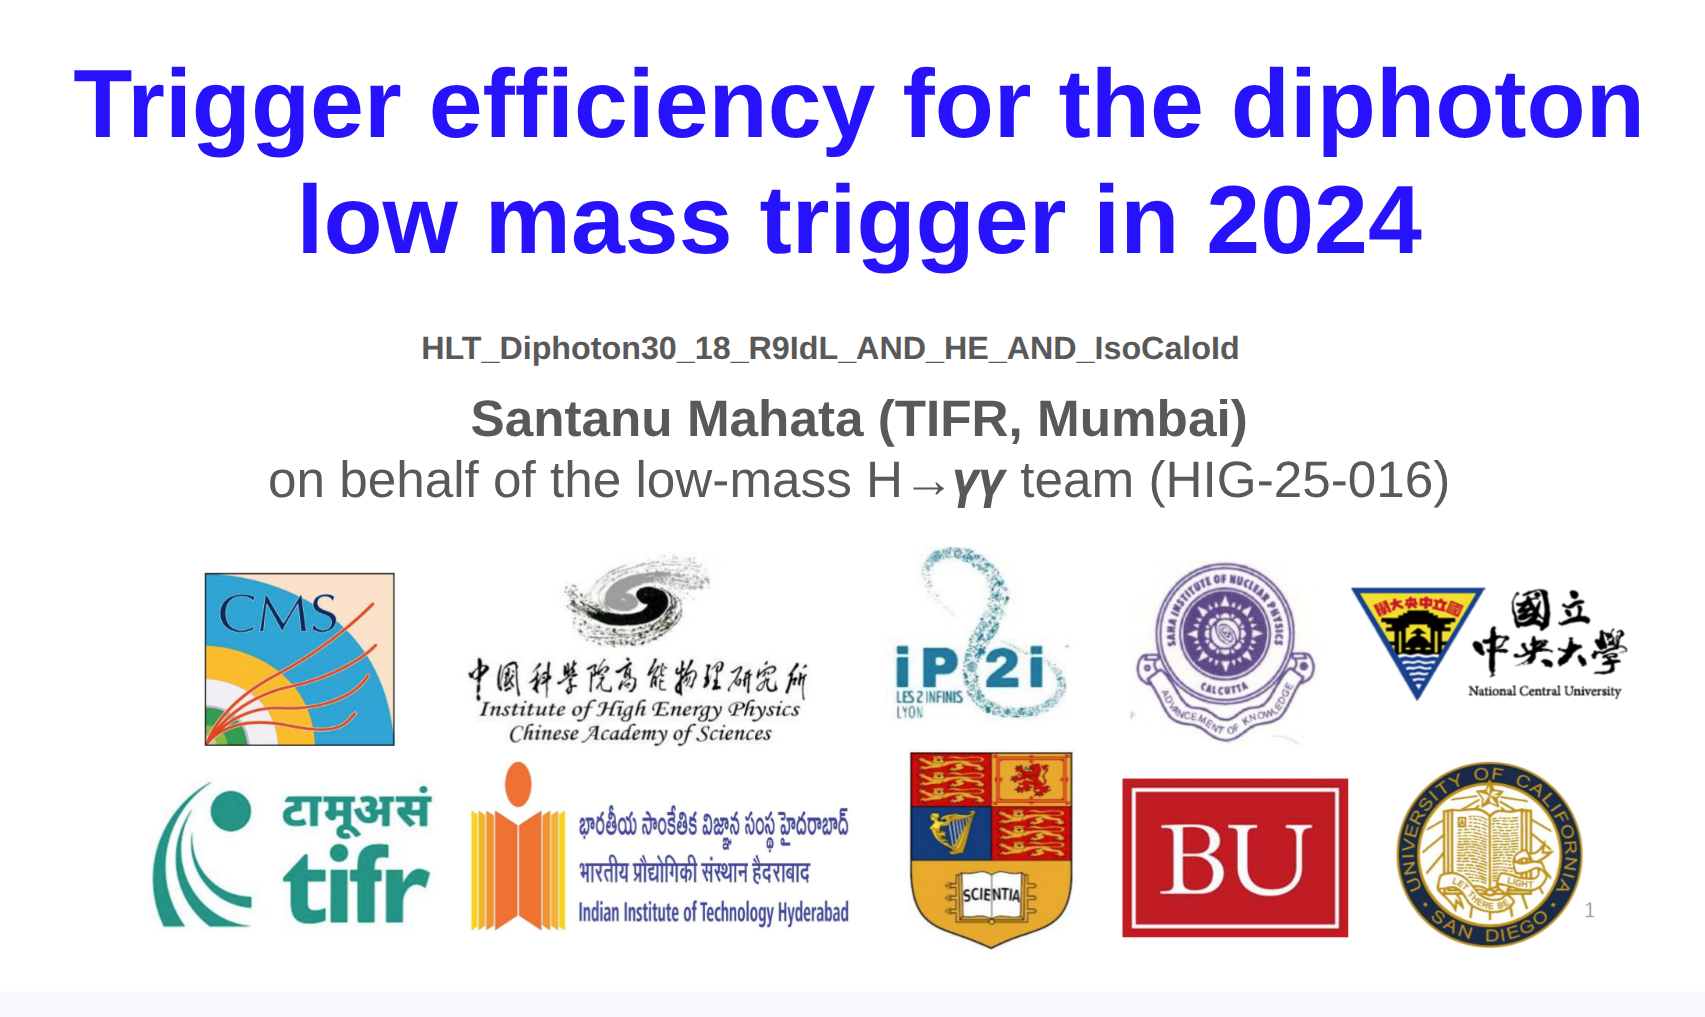
\includegraphics[width=\paperwidth,height=\paperheight,keepaspectratio]{firstslide.png}};
  \end{tikzpicture}
\end{frame}}

\begin{frame}{Choosing HLT according to the physics}
  \centering
  \resizebox{0.97\linewidth}{!}{%
  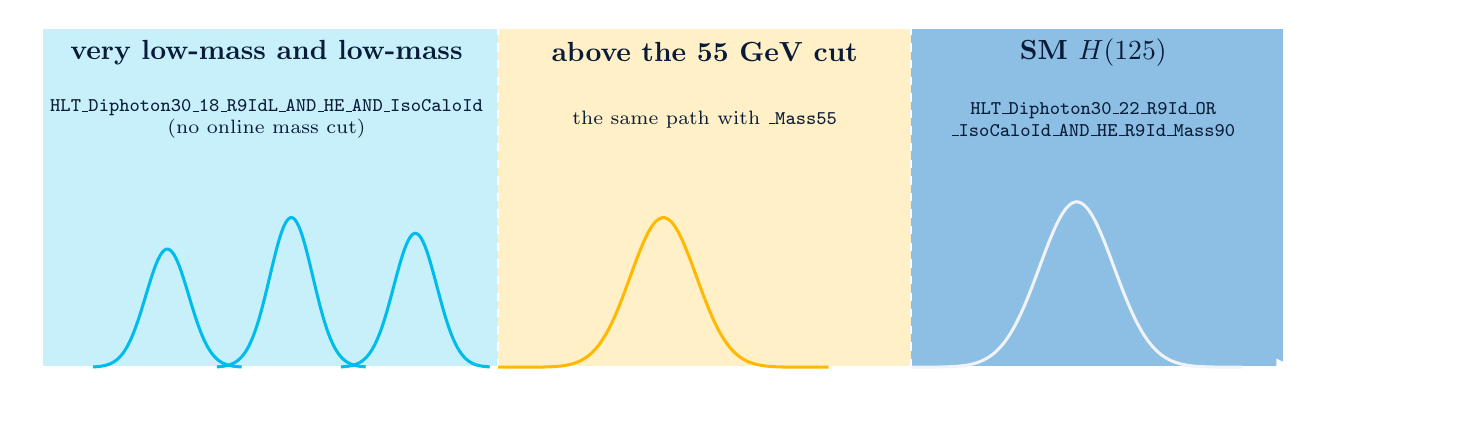
\begin{tikzpicture}[
      declare function={pk(\x,\m,\s)=exp(-((\x-\m)^2)/(2*\s*\s));}]
    \def\sx{0.105}   % cm per GeV

    % shaded mass bands
    \fill[cmsaccent!22]  (0,0) rectangle (55*\sx,4.3);
    \fill[cmsgold!22]    (55*\sx,0) rectangle (105*\sx,4.3);
    \fill[cmsblue!45]    (105*\sx,0) rectangle (150*\sx,4.3);

    % axis
    \draw[white,line width=1pt,-{Latex[length=3mm]}] (0,0) -- (152*\sx,0)
      node[right,white] {$m_{\gamma\gamma}$ [GeV]};
    \foreach \m in {0,20,40,60,80,100,120,140}{
      \draw[white,line width=0.7pt] (\m*\sx,0) -- (\m*\sx,-0.16)
        node[below,white,font=\small] {\m};}
    \draw[white,dashed,line width=0.7pt] (55*\sx,0) -- (55*\sx,4.3);
    \draw[white,dashed,line width=0.7pt] (105*\sx,0) -- (105*\sx,4.3);

    % illustrative signal peaks
    \foreach \m/\h in {15/1.5, 30/1.9, 45/1.7}{
      \draw[cmsaccent,line width=1.1pt,smooth,domain=\m-9:\m+9,samples=90]
        plot (\x*\sx,{\h*pk(\x,\m,2.6)});}
    \draw[cmsgold,line width=1.1pt,smooth,domain=55:95,samples=120]
      plot (\x*\sx,{1.9*pk(\x,75,4.0)});
    \draw[offwhite,line width=1.1pt,smooth,domain=105:145,samples=120]
      plot (\x*\sx,{2.1*pk(\x,125,4.5)});

    % band labels
    \node[navydark,align=center,font=\bfseries] at (27*\sx,4.0)
      {very low-mass and low-mass};
    \node[navydark,align=center,font=\bfseries]   at (80*\sx,4.0) {above the 55~GeV cut};
    \node[navydark,align=center,font=\bfseries]   at (127*\sx,4.0) {SM $H(125)$};

    % path labels
    \node[navydark,align=center,font=\scriptsize] at (27*\sx,3.15)
      {\texttt{HLT\_Diphoton30\_18\_R9IdL\_AND\_HE\_AND\_IsoCaloId}\\ (no online mass cut)};
    \node[navydark,align=center,font=\scriptsize]   at (80*\sx,3.15)
      {the same path with \texttt{\_Mass55}};
    \node[navydark,align=center,font=\scriptsize]  at (127*\sx,3.15)
      {\texttt{HLT\_Diphoton30\_22\_R9Id\_OR}\\ \texttt{\_IsoCaloId\_AND\_HE\_R9Id\_Mass90}};
  \end{tikzpicture}}

  \vspace{4pt}
  \begin{itemize}\footnotesize\itemsep2pt
    \item An online $m_{\gamma\gamma}$ requirement cuts away exactly the region a search below it
          needs --- so the \hl{no-mass-cut} path is the one that works for the very low-mass and low-mass searches,
          and it is the path measured here.
    \item Above the cut the \texttt{\_Mass55} variant is usable, and the SM \Hgg{} analyses run on
          the \texttt{\_Mass90} path.
  \end{itemize}
  \vfill
  {\tiny\color{lightgrey} Peak positions and widths are illustrative, not measured line shapes.}
\end{frame}

\begin{frame}{The HLT path: reading the name, and the filter sequence}
  \vspace{0pt}\par
  \centering
  {\small\texttt{%
    \textcolor{offwhite}{HLT\_}%
    \textcolor{cmsaccent}{Diphoton}%
    \textcolor{cmsgold}{30\_18}%
    \textcolor{offwhite}{\_}%
    \textcolor{cmsaccent}{R9IdL}%
    \textcolor{offwhite}{\_AND\_}%
    \textcolor{cmsgold}{HE}%
    \textcolor{offwhite}{\_AND\_}%
    \textcolor{cmsaccent}{IsoCaloId}}}

  \vspace{4pt}
  {\scriptsize
  \begin{tabular}{@{}l@{\hspace{4pt}}p{0.31\linewidth}@{\hspace{10pt}}l@{\hspace{4pt}}p{0.31\linewidth}@{}}
    \texttt{\textcolor{offwhite}{HLT\_}} & runs on the full event, after the L1 accept &
    \texttt{\textcolor{cmsaccent}{R9IdL}} & \RNine{} identification, loose working point \\
    \texttt{\textcolor{cmsaccent}{Diphoton}} & two photon candidates: one seeded, one unseeded leg &
    \texttt{\textcolor{cmsgold}{HE}} & hadronic-over-electromagnetic filter \\
    \texttt{\textcolor{cmsgold}{30\_18}} & the two \pT{} thresholds in GeV &
    \texttt{\textcolor{cmsaccent}{IsoCaloId}} & shower shape and calorimeter isolation \\
  \end{tabular}}

  \vspace{3pt}
  \begin{minipage}{0.95\linewidth}\raggedright\scriptsize
    \gold{No \texttt{\_Mass} suffix} --- this path applies no online $m_{\gamma\gamma}$ cut,
    which is why it is the one usable below 55~GeV.\\
    \textbf{L1 seed} (\texttt{hltL1sSingleAndDoubleEGor}) --- the OR of the single- and
    double-EG seeds.
  \end{minipage}

  \vspace{3pt}
  \centering
  \resizebox{0.97\linewidth}{!}{%
  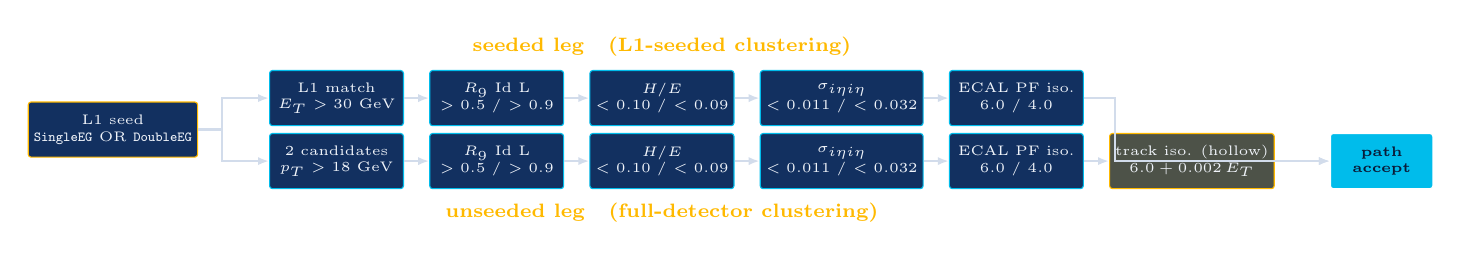
\begin{tikzpicture}[
      font=\tiny,
      node distance=3.2mm,
      box/.style={draw=cmsaccent, fill=navymid, text=offwhite, rounded corners=1pt,
                  minimum height=7mm, minimum width=17mm, inner xsep=2pt,
                  inner ysep=2pt, align=center},
      seedbox/.style={box, draw=cmsgold},
      trkbox/.style={box, draw=cmsgold, fill=cmsgold!25!navymid},
      endbox/.style={box, draw=white, fill=cmsaccent, text=navydark, font=\tiny\bfseries},
      flow/.style={-{Latex[length=1.4mm]}, draw=lightgrey, thick},
      lbl/.style={text=cmsgold, font=\scriptsize\bfseries}]

    % --- L1 ---
    \node[seedbox] (l1) {L1 seed\\ \texttt{SingleEG} OR \texttt{DoubleEG}};

    % --- seeded chain (upper row) ---
    \node[box, above right=4mm and 9mm of l1.east, anchor=west] (s1)
      {L1 match\\ $E_{T}>30$~GeV};
    \node[box, right=of s1] (s2) {\RNine{} Id L\\ $>0.5$ / $>0.9$};
    \node[box, right=of s2] (s3) {$H/E$\\ $<0.10$ / $<0.09$};
    \node[box, right=of s3] (s4) {$\sigma_{i\eta i\eta}$\\ $<0.011$ / $<0.032$};
    \node[box, right=of s4] (s5) {ECAL PF iso.\\ $6.0$ / $4.0$};

    % --- unseeded chain (lower row) ---
    \node[box, below right=4mm and 9mm of l1.east, anchor=west] (u1)
      {2 candidates\\ $p_{T}>18$~GeV};
    \node[box, right=of u1] (u2) {\RNine{} Id L\\ $>0.5$ / $>0.9$};
    \node[box, right=of u2] (u3) {$H/E$\\ $<0.10$ / $<0.09$};
    \node[box, right=of u3] (u4) {$\sigma_{i\eta i\eta}$\\ $<0.011$ / $<0.032$};
    \node[box, right=of u4] (u5) {ECAL PF iso.\\ $6.0$ / $4.0$};
    \node[trkbox, right=of u5] (u6) {track iso. (hollow)\\ $6.0+0.002\,E_{T}$};

    % --- accept ---
    \node[endbox, right=7mm of u6.east, anchor=west,
          minimum width=13mm] (acc) {path\\ accept};

    % --- row labels ---
    \node[lbl, left=1mm of s1.west, anchor=east, xshift=-1mm] {};
    \node[lbl, above=0.5mm of s3] {seeded leg \; (L1-seeded clustering)};
    \node[lbl, below=0.5mm of u3] {unseeded leg \; (full-detector clustering)};

    % --- arrows ---
    \draw[flow] (l1.east) -- ++(3mm,0) |- (s1.west);
    \draw[flow] (l1.east) -- ++(3mm,0) |- (u1.west);
    \foreach \a/\b in {s1/s2, s2/s3, s3/s4, s4/s5,
                       u1/u2, u2/u3, u3/u4, u4/u5, u5/u6}
      \draw[flow] (\a) -- (\b);
    \draw[flow] (s5.east) -- ++(4mm,0) |- (acc.west);
    \draw[flow] (u6.east) -- ++(4mm,0) |- (acc.west);
  \end{tikzpicture}}
  \par\vspace{2pt}
  \begin{minipage}{0.95\linewidth}\raggedright\scriptsize
    Both legs must fire, so they are measured \gold{separately}; the
    \hl{hollow track isolation} exists only on the unseeded leg. EB\,/\,EE thresholds shown.
  \end{minipage}
\end{frame}

\begin{frame}{Offline photon preselection for 2024 (same as 2023), and the binning}
  \centering
  {\footnotesize
  \begin{tabular}{@{}lccccc@{}}
    \toprule
    \textbf{Category} & $H/E$ & $\sigma_{i\eta i\eta}$ & \RNine{} & \texttt{Rho\_PfPhoISO03} & \texttt{TrackerISO03} \\
    \midrule
    Barrel, $\RNine < 0.85$ & $< 0.08$ & $< 0.011$ & $> 0.5$ & $< 3.0$ & $< 6.0$ \\
    Barrel, $\RNine > 0.85$ & $< 0.08$ & $< 0.011$ & $> 0.5$ & $< 3.0$ & $< 6.0$ \\
    Endcap, $\RNine > 0.9$  & $< 0.08$ & $< 0.032$ & $> 0.9$ & $< 3.0$ & $< 6.0$ \\
    \bottomrule
  \end{tabular}}

  \vspace{7pt}
  {\footnotesize
  \begin{tabular}{@{}lcl@{}}
    \toprule
    \textbf{Leg} & \textbf{Bins} & \textbf{Probe $E_{T}$ bin edges [GeV]} \\
    \midrule
    seeded (30~GeV)   & 9  & 0, 35, 37, 40, 45, 50, 60, 70, 90, $\infty$ \\
    unseeded (18~GeV) & 12 & 0, 21, 25, 28, 31, 35, 40, 45, 50, 60, 70, 90, $\infty$ \\
    \midrule
    \multicolumn{3}{@{}l@{}}{\textbf{5 \RNine{}/$\eta$ categories on each leg:}\;
      EB $0.50$--$0.55$, EB $0.55$--$0.85$, EB $>0.85$, EE $0.90$--$0.93$, EE $>0.93$} \\
    \bottomrule
  \end{tabular}}
  \vspace{4pt}

\end{frame}
\begin{frame}{Why an $\eta$--\RNine{} reweighting}
  \begin{columns}[T,onlytextwidth]
    \column{0.40\textwidth}
      \begin{itemize}
        \item The shower shapes of photons and electrons are different.
        \item The efficiency is derived with electrons ($Z\to ee$), so it has to be corrected for the difference in shower shape.
        \item The correction is applied as a weight in bins of $|\eta|$ and \RNine{}.
      \end{itemize}
    \column{0.58\textwidth}\centering\wimg{0.96\linewidth}{maps/map_2024_with_NF.pdf}
  \end{columns}
  \vspace{2pt}
  {\tiny\color{lightgrey} $\eta$--\RNine{} weight map, 2024 with NF.}
\end{frame}

\begin{frame}{Tag-and-probe method}
  \begin{itemize}
    \item \gold{Sample:} \Zee{} events in 2024 data; electrons are used as photon proxies
          since the online filters are photon-like (no pixel-veto at HLT here).
    \item \gold{Tag:} tightly identified, trigger-matched electron.
          \gold{Probe:} the other leg, unbiased with respect to the filter under test.
    \item Efficiency per (leg, ECAL region, \RNine{} bin, probe-\pT{} bin) from a
          \hl{fit} of the tag--probe invariant-mass distribution in the
          passing and failing categories. It is the \gold{efficiency of the probe} ---
          $N_{\text{pass}}$ and $N_{\text{fail}}$ count \gold{probes} that do and do not
          pass the filter under test:
          \[
            \varepsilon_{\text{probe}}
            =\frac{N^{\text{probe}}_{\text{pass}}}
                  {N^{\text{probe}}_{\text{pass}}+N^{\text{probe}}_{\text{fail}}}
          \]
    \item \gold{Tag trigger:} \texttt{HLT\_Ele30\_WPTight\_Gsf}, tag matched to the filter of this trigger.
    \item \gold{\pT{} cuts:} tag $\pT>35$~GeV; probe $\pT>30$~GeV (seeded leg) and $\pT>18$~GeV (unseeded leg).
    \item \gold{Signal model:} Breit--Wigner $\otimes$ double-sided Crystal Ball (\texttt{bwDscb}).
    \item \gold{Background:} \hl{RooCMSShape} (nominal) --- an \hl{Exponential} fit is also run
          and is used as the fit-model variation.
    \item An \gold{$\eta$--\RNine{} reweighting} and a \gold{scale correction} are applied to
          the sample before fitting.
  \end{itemize}
\end{frame}
\begin{frame}{Example tag-and-probe mass fits}
  \centering
  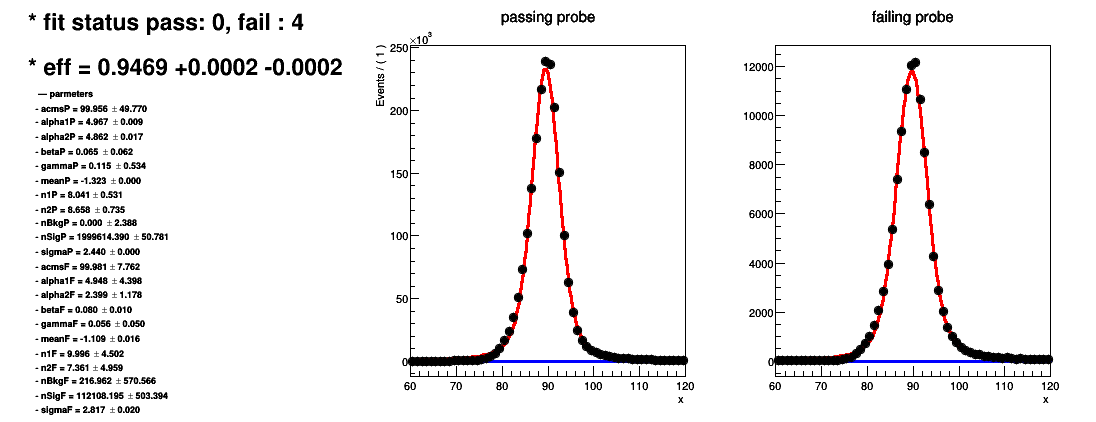
\includegraphics[width=0.7\linewidth,height=0.68\textheight,keepaspectratio]
    {method/fit_seeded_EB_R9_0p55to0p85_pt40to45.png}\\
  {\tiny\color{lightgrey} seeded, EB $0.55<\RNine<0.85$, $40<\pT<45$~GeV}\par
  \vspace{4pt}
  {\footnotesize\color{lightgrey} Passing and failing categories fitted;
   bwDscb signal, RooCMSShape background.}
\end{frame}
\begin{frame}{2024 dataset}
  \textbf{Data:} \hl{\texttt{/EGamma0/*}} and \hl{\texttt{/EGamma1/*}} MINIAOD,
  \gold{PromptReco}, eras \gold{C--I}:
  \\[4pt]
  {\footnotesize
  \begin{tabular}{@{}ll@{}}
    \texttt{/EGamma0/Run2024C-PromptReco-v1/MINIAOD} & \texttt{/EGamma1/Run2024C-PromptReco-v1/MINIAOD}\\
    \texttt{/EGamma0/Run2024D-PromptReco-v1/MINIAOD} & \texttt{/EGamma1/Run2024D-PromptReco-v1/MINIAOD}\\
    \texttt{/EGamma0/Run2024E-PromptReco-v1/MINIAOD} & \texttt{/EGamma1/Run2024E-PromptReco-v1/MINIAOD}\\
    \texttt{/EGamma0/Run2024E-PromptReco-v2/MINIAOD} & \texttt{/EGamma1/Run2024E-PromptReco-v2/MINIAOD}\\
    \texttt{/EGamma0/Run2024F-PromptReco-v1/MINIAOD} & \texttt{/EGamma1/Run2024F-PromptReco-v1/MINIAOD}\\
    \texttt{/EGamma0/Run2024G-PromptReco-v1/MINIAOD} & \texttt{/EGamma1/Run2024G-PromptReco-v1/MINIAOD}\\
    \texttt{/EGamma0/Run2024H-PromptReco-v1/MINIAOD} & \texttt{/EGamma1/Run2024H-PromptReco-v1/MINIAOD}\\
    \texttt{/EGamma0/Run2024I-PromptReco-v1/MINIAOD} & \texttt{/EGamma1/Run2024I-PromptReco-v1/MINIAOD}\\
    \texttt{/EGamma0/Run2024I-PromptReco-v2/MINIAOD} & \texttt{/EGamma1/Run2024I-PromptReco-v2/MINIAOD}\\
  \end{tabular}}
  \\[6pt]
  \begin{itemize}\footnotesize
    \item Photon energy scale \& smearing applied from the Summer24 NanoAODv15 EGM
          \texttt{photonSS\_EtDependent} correction set.
    \item 2024 is treated as a \gold{single era} --- no pre/post split, unlike 2022
          (preEE/postEE) and 2023 (pre/postBPix).
  \end{itemize}
\end{frame}

\begin{frame}{2024 efficiency with NF --- seeded and unseeded legs}
  \begin{columns}[T,onlytextwidth]
    \column{0.49\textwidth}\centering\wimg{\linewidth}{eff/eff2024_withNF_seeded.pdf}
    \column{0.49\textwidth}\centering\wimg{\linewidth}{eff/eff2024_withNF_unseeded.pdf}
  \end{columns}
  \vspace{2pt}
  {\tiny\color{lightgrey} Data efficiency vs probe \ET, 2024 with NF; the five \RNine/$\eta$ categories overlaid. Nominal fit. Error bars: stat $\oplus$ syst.}
\end{frame}
\begin{frame}{Inspecting the effect of normalising flow corrections}
  \centering
  {\scriptsize
  \begin{tabular}{@{}p{0.2\linewidth}p{0.5\linewidth}@{}}
    \toprule
    \textbf{Set} & \textbf{$\eta$--\RNine{} reweighting map} \\
    \midrule
    \textcolor{cmsgreen}{\textbf{2023 (postBPix)}} & with flow-corrected $\eta$--\RNine{} reweighting map \\
    \textcolor{cmsaccent}{\textbf{2024 without NF}} & without flow-corrected $\eta$--\RNine{} reweighting map \\
    \textcolor{red!70!white}{\textbf{2024 with NF}} & with flow-corrected $\eta$--\RNine{} reweighting map \\
    \bottomrule
  \end{tabular}}
\end{frame}
\begin{frame}[label=eff-seed-EB]{2023 vs 2024 without NF vs 2024 with NF --- seeded leg, EB bins}
  \begin{columns}[T,onlytextwidth]
    \column{0.33\textwidth}\centering\effpanel{normal}{seed}{EB}{R9_0p50to0p55}
    \column{0.33\textwidth}\centering\effpanel{normal}{seed}{EB}{R9_0p55to0p85}
    \column{0.33\textwidth}\centering\effpanel{normal}{seed}{EB}{R9gt0p85}
  \end{columns}
  \vspace{2pt}
  {\tiny\color{lightgrey} Error bars: stat $\oplus$ syst. Lower pad: ratio to 2024 without NF, the two uncertainties added in quadrature.}
\end{frame}
\begin{frame}[label=eff-seed-EE]{2023 vs 2024 without NF vs 2024 with NF --- seeded leg, EE bins}
  \begin{columns}[T,onlytextwidth]
    \column{0.44\textwidth}\centering\effpanel{normal}{seed}{EE}{R9_0p90to0p93}
    \column{0.44\textwidth}\centering\effpanel{normal}{seed}{EE}{R9gt0p93}
  \end{columns}
  \vspace{2pt}
  {\tiny\color{lightgrey} Error bars: stat $\oplus$ syst. Lower pad: ratio to 2024 without NF, the two uncertainties added in quadrature.}
\end{frame}
\begin{frame}[label=eff-unseed-EB]{2023 vs 2024 without NF vs 2024 with NF --- unseeded leg, EB bins}
  \begin{columns}[T,onlytextwidth]
    \column{0.33\textwidth}\centering\effpanel{normal}{unseed}{EB}{R9_0p50to0p55}
    \column{0.33\textwidth}\centering\effpanel{normal}{unseed}{EB}{R9_0p55to0p85}
    \column{0.33\textwidth}\centering\effpanel{normal}{unseed}{EB}{R9gt0p85}
  \end{columns}
  \vspace{2pt}
  {\tiny\color{lightgrey} Error bars: stat $\oplus$ syst. Lower pad: ratio to 2024 without NF, the two uncertainties added in quadrature.}
\end{frame}
\begin{frame}[label=eff-unseed-EE]{2023 vs 2024 without NF vs 2024 with NF --- unseeded leg, EE bins}
  \begin{columns}[T,onlytextwidth]
    \column{0.44\textwidth}\centering\effpanel{normal}{unseed}{EE}{R9_0p90to0p93}
    \column{0.44\textwidth}\centering\effpanel{normal}{unseed}{EE}{R9gt0p93}
  \end{columns}
  \vspace{2pt}
  {\tiny\color{lightgrey} Error bars: stat $\oplus$ syst. Lower pad: ratio to 2024 without NF, the two uncertainties added in quadrature.}
\end{frame}
\begin{frame}{Map without NF vs map with NF}
  \begin{columns}[T,onlytextwidth]
    \column{0.5\textwidth}\centering\wimg{\linewidth}{maps/map_old_map_2024_repo.pdf}
    \column{0.5\textwidth}\centering\wimg{\linewidth}{maps/map_new_map_2024_local.pdf}
  \end{columns}
  \vspace{4pt}
  \begin{itemize}\scriptsize
    \item Without NF: Hgg / DY MC, density-normalised, empty-DY cell $\to$ 1 (\texttt{.meta} file). Range 0.42--5.29; 118 cells exactly 1.
    \item With NF: no metadata file; recorded as ``used as supplied'' at weight replacement. Range 0--5.93; 4 cells exactly 0.
  \end{itemize}
\end{frame}
\begin{frame}{Probe \RNine{} before and after the $\eta$--\RNine{} reweighting --- seeded leg}
  \begin{columns}[T,onlytextwidth]
    \column{0.5\textwidth}\centering\wimg{\linewidth}{r9/r9_before_after_seed_EB_pass.pdf}
    \column{0.5\textwidth}\centering\wimg{\linewidth}{r9/r9_before_after_seed_EE_pass.pdf}
  \end{columns}
  \vspace{2pt}
  {\tiny\color{lightgrey} Passing probes of the normal-set fits, $60<m_{ee}<120$~GeV. Black: unweighted. Blue: weighted with the map without NF. Red: weighted with the map with NF. Each curve normalised to its total. Dashed lines: fit-category boundaries.}
\end{frame}
\begin{frame}{Probe \RNine{} before and after the $\eta$--\RNine{} reweighting --- unseeded leg}
  \begin{columns}[T,onlytextwidth]
    \column{0.5\textwidth}\centering\wimg{\linewidth}{r9/r9_before_after_unseed_EB_pass.pdf}
    \column{0.5\textwidth}\centering\wimg{\linewidth}{r9/r9_before_after_unseed_EE_pass.pdf}
  \end{columns}
  \vspace{2pt}
  {\tiny\color{lightgrey} Passing probes of the normal-set fits, $60<m_{ee}<120$~GeV. Black: unweighted. Blue: weighted with the map without NF. Red: weighted with the map with NF. Each curve normalised to its total. Dashed lines: fit-category boundaries.}
\end{frame}

\begin{frame}{Summary}
  \begin{itemize}
    \item 2024 HLT efficiencies of the seeded and unseeded legs derived with tag-and-probe on \Zee{}, using the $\eta$--\RNine{} reweighting map without and with the normalising-flow (NF) correction.
    \item Efficiencies compared as a function of probe \ET{}: 2023, 2024 without NF and 2024 with NF.
    \item The two maps compared cell by cell; probe \RNine{} distributions shown before and after reweighting for each map.
    \item Effect of NF on the efficiencies is bin dependent:
      \begin{itemize}
        \item barrel: negligible;
        \item endcap: significantly larger than in any other bin, especially around the turn-on in probe \pT{}.
      \end{itemize}
    \item Status: the 2023 trigger efficiencies are blessed by EGM; the 2024 efficiencies (without NF) have been \href{https://indico.cern.ch/event/1727810/contributions/7279108/attachments/3345810/5997817/Trigger\%20efficiency\%20for\%20the\%20diphoton\%20low\%20mass\%20trigger\%20in\%202024\%20HLT_Diphoton30_18_R9IdL_AND_HE_AND_IsoCaloId.pdf}{presented to EGM} and are waiting for approval.
  \end{itemize}
\end{frame}
% ── Backup ───────────────────────────────────────────────────
\appendix
\partdivider{~}{Backup}

\begin{frame}{The HLT filter chain --- online cuts (2024 sequence)}
  \centering
  {\footnotesize
  \begin{tabular}{@{}llcc@{}}
    \toprule
    \textbf{Filter} & \textbf{Variable} & \textbf{EB} & \textbf{EE}\\
    \midrule
    $E_{T}$ (seeded)          & \texttt{HLTEgammaEtFilter}      & $>30$~GeV & $>30$~GeV\\
    $p_{T}$ (unseeded)        & \texttt{HLT1Photon}             & $>18$~GeV & $>18$~GeV\\
    \RNine{} Id ``L''         & \texttt{r95x5}                  & $>0.5$ & $>0.9$\\
    $H/E$                     & \texttt{hltEgammaHoverE}        & $<0.10\cdot E$ & $<0.09\cdot E$\\
    Cluster shape             & $\sigma_{i\eta i\eta}$ (5$\times$5) & $<0.011$ & $<0.032$\\
    ECAL PF-cluster iso.      & \texttt{EcalPFClusterIso}       & $<6.0 + 0.012\,E_{T}$ & $<4.0 + 0.012\,E_{T}$\\
    Track iso. \gold{(unseeded only)} & hollow track iso.       & $<6.0 + 0.002\,E_{T}$ & $<6.0 + 0.002\,E_{T}$\\
    \bottomrule
  \end{tabular}}
  \\[8pt]
  {\footnotesize\color{lightgrey}
   Thresholds read directly from the 2024 filter-sequence dump
   (\texttt{thrRegular*} / \texttt{thrOverE*} of each \texttt{HLTEgammaGeneric[Quadratic]Filter}).}
\end{frame}

\begin{frame}{Where the 2024 efficiency moved: with NF $-$ without NF, every bin}
  \plotslide[0.95]{diff/heat_local_minus_repo_normal.pdf}
    {Top: absolute difference. Bottom: difference / ($\sigma_{\rm without\,NF}\oplus\sigma_{\rm with\,NF}$), $\sigma$ = stat $\oplus$ syst; both fits use the same events, so this treats correlated numbers as independent.}
  \vspace{-6pt}
  {\scriptsize Mean $|\Delta|$ = 0.0048 over 105 bins. 10 bins with $|\Delta|>0.01$: 9 unseeded, 8 of them with $\ET<31$~GeV. Largest $|\Delta|/\sigma$: 1.65.}
\end{frame}
\begin{frame}{$\eta$--\RNine{} map, 2023 postBPix vs 2024 with NF}
  \begin{columns}[T,onlytextwidth]
    \column{0.5\textwidth}\centering\wimg{\linewidth}{maps/map_2023_postBPix.pdf}
    \column{0.5\textwidth}\centering\wimg{\linewidth}{maps/map_2024_with_NF.pdf}
  \end{columns}
  \vspace{4pt}
  {\scriptsize\color{lightgrey} Same 25$\times$16 binning. Range: 2023 postBPix 0.00--5.63, 2024 with NF 0.00--5.93. Cells exactly 0: 4 and 4, 0 in common.}
\end{frame}
\begin{frame}{2024 with NF vs 2023 postBPix, cell by cell}
  \begin{columns}[T,onlytextwidth]
    \column{0.5\textwidth}\centering\wimg{\linewidth}{maps/map_2024_with_NF_over_2023.pdf}
    \column{0.5\textwidth}\centering\wimg{\linewidth}{maps/map_2024_with_NF_minus_2023.pdf}
  \end{columns}
  \vspace{4pt}
  {\scriptsize\color{lightgrey} Left: ratio 2024 / 2023 (empty where the 2023 cell is 0). Right: difference 2024 $-$ 2023. In the 282 cells of the analysis categories: ratio 0.70--1.91, mean $|$difference$|$ 0.071, largest 1.36.}
\end{frame}
\begin{frame}{Map slices, 2023 postBPix vs 2024 with NF}
  \plotslide[0.80]{maps/map_slices_vs_r9_2023_vs_2024.pdf}
    {Weight vs \RNine{} bin in every $|\eta|$ row. Shaded: the \RNine{} windows of the analysis categories in EB and EE rows.}
\end{frame}
\begin{frame}{With NF $-$ without NF, cell by cell}
  \plotslide[0.92]{maps/map_new_old_diff.pdf}
    {Drawn in bin-index space (\RNine{} bins are 0.5, 0.05, 0.02 and 0.01 wide); dashed lines bound the EB--EE gap row. with NF / without NF ranges 0 to 4.62.}
\end{frame}
\begin{frame}{Map slices: weight vs \RNine{} in every $|\eta|$ row}
  \plotslide[0.80]{maps/map_slices_vs_r9.pdf}
    {Shaded: the \RNine{} windows of the analysis categories in EB and EE rows.}
\end{frame}
\begin{frame}{Which cells the probes actually use}
  \centering
  \wimg{0.98\linewidth}{why/occupancy_seed.pdf}\\[2pt]
  \wimg{0.98\linewidth}{why/occupancy_unseed.pdf}\\[2pt]
  {\tiny\color{lightgrey} Selected probes per map cell (normal set, pass+fail, $60<m<120$~GeV), top seeded, bottom unseeded. Hatched: map without NF $=1$ (\texttt{//}), map with NF $=0$ (\texttt{xx}). Selected probes in either kind of cell: 0 in every category.}
\end{frame}
% ── Part: why ────────────────────────────────────────────────
\partdivider{Backup}{Do the weights explain the shifts?}

\begin{frame}{Per-probe weights and effective statistics}
  \plotslide[0.95]{why/weights_and_neff.pdf}
    {Left: per-probe weight distribution of all selected probes. Right: effective number of failing probes $N_{\rm eff}=(\sum w)^2/\sum w^2$, with NF / without NF, per bin: 0.92--1.01.}
\end{frame}

\begin{frame}{Method: what the weights alone do}
  \begin{itemize}\footnotesize
    \item Both weights are a pure lookup in the map: every selected probe's stored weight equals its cell value
          (0 mismatches in 2$\times$159.9\,M entries, without and with NF).
    \item So, per fitter bin, count probes per map cell once, separately for pass and fail. Any map then gives
          \[ P=\sum_c N^{\rm pass}_c\,w_c,\qquad F=\sum_c N^{\rm fail}_c\,w_c,\qquad
             \varepsilon_{\rm count}=\frac{P}{P+F}. \]
    \item Cuts, flags and \ET{} bins parsed from the 20 settings files; $60<m<120$~GeV.
          Rebuilt yields equal the sums of stored weights to $1.4\times10^{-8}$ (relative).
    \item $\varepsilon_{\rm count}$ includes background --- it is \hl{not} the fitted efficiency.
          $\Delta\varepsilon_{\rm count}=\varepsilon^{\rm with\,NF}_{\rm count}-\varepsilon^{\rm without\,NF}_{\rm count}$ is the change from the map alone, with no fit.
  \end{itemize}
\end{frame}

\begin{frame}{Fitted shift vs shift from the weights alone --- unseeded}
  \plotslide[0.98]{why/fit_vs_count_vs_pt_normal_unseed.pdf}
    {Red: fitted with NF $-$ without NF. Black: $\Delta\varepsilon_{\rm count}$. Grey: $\pm(\sigma_{\rm without\,NF}\oplus\sigma_{\rm with\,NF})$, stat $\oplus$ syst.}
  \vspace{-4pt}
  {\scriptsize Largest $|\Delta\varepsilon_{\rm count}|$ in any bin: 0.0048 (normal), 0.0043 (fullPath). Largest fitted $|\Delta|$: 0.114.}
\end{frame}

\begin{frame}{Every bin: fitted shift vs counting shift; normal vs fullPath}
  \begin{columns}[T,onlytextwidth]
    \column{0.38\textwidth}\centering\wimg{\linewidth}{why/fit_vs_count_scatter_normal.pdf}
    \column{0.62\textwidth}\centering\wimg{\linewidth}{why/normal_vs_fullPath_shifts.pdf}
  \end{columns}
  \vspace{2pt}
  {\scriptsize Correlation of fitted and counting shift: 0.18 (normal), 0.56 (fullPath).
   Same map, extra \texttt{probe\_passFullPath==1}: largest fitted $|\Delta|$ 0.114 (normal) vs 0.0083 (fullPath).}
\end{frame}

\begin{frame}{The six largest fitted shifts, cell by cell}
  \plotslide[0.92]{why/cell_decomposition_top6.pdf}
    {First-order contribution of each cell to $\Delta\varepsilon_{\rm count}$; $\Sigma$ cells vs exact counting shift in each title.}
  \vspace{-6pt}
  {\scriptsize In 4 of the 6, $\Delta\varepsilon_{\rm count}$ has the opposite sign to the fitted shift; in all 6, $|\Delta\varepsilon_{\rm count}|\le0.0048$.}
\end{frame}

\begin{frame}{Mean weight of passing vs failing probes --- unseeded}
  \plotslide[0.98]{why/wpass_over_wfail_unseed.pdf}
    {$\varepsilon_{\rm count}$ changes only through $\langle w\rangle_{\rm pass}/\langle w\rangle_{\rm fail}$; shown for both maps.}
\end{frame}

\begin{frame}{The largest shift in the fit: unseeded EE $\RNine>0.93$, $\ET<21$~GeV}
  \centering
  \colorbox{white}{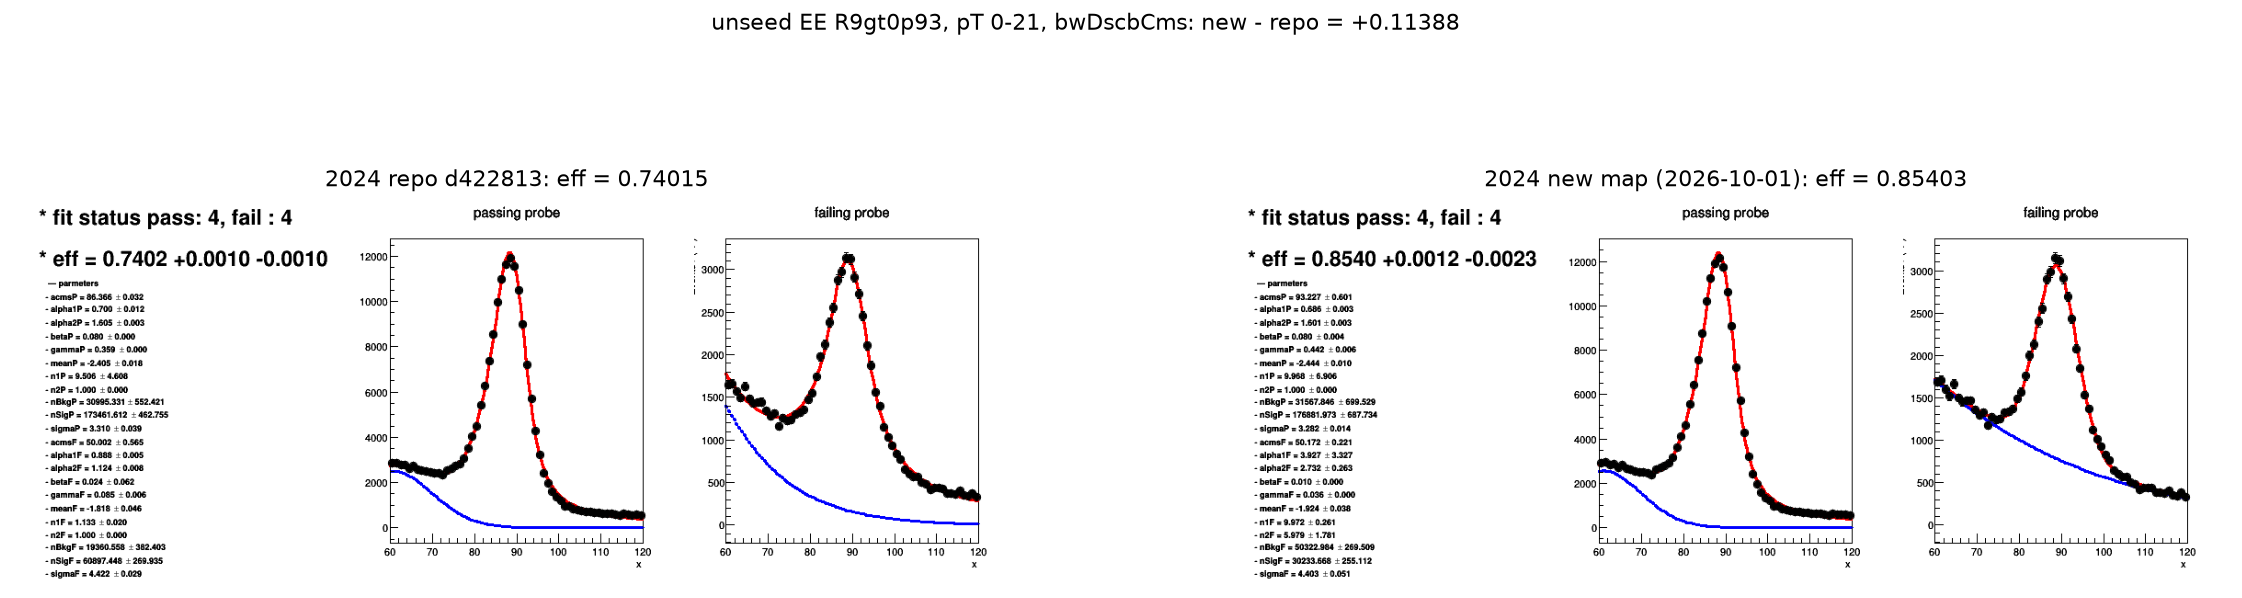
\includegraphics[width=0.98\linewidth,height=0.55\textheight,keepaspectratio]{why/fit_shift1_unseed_EE_R9gt0p93_0_bwDscbCms.png}}\\[3pt]
  {\scriptsize Left without NF, right with NF. Both print \texttt{fit status pass: 4, fail: 4}.
   Failing-probe fit: background yield 19\,361 $\to$ 50\,323, signal yield 60\,897 $\to$ 30\,234 (values printed on the plots).
   Counting shift for this bin: $+0.0030$; fitted shift $+0.114$.}
\end{frame}

\begin{frame}{From map to fitted efficiency: three stages}
  \begin{itemize}\footnotesize
    \item \gold{1. Map $\to$ weighted yields.} Per fitter bin, pass and fail: total of the mass histogram in 60--120~GeV, with NF / without NF.
          Equal to the yields rebuilt from per-cell probe counts to $1.5\times10^{-5}$ (relative).
    \item \gold{2. Weighted yields $\to$ mass templates.} The pass / fail histograms the fitter fitted, without vs with NF:
          shape compared by the total-variation distance TV $=\frac12\sum|p_{\rm with\,NF}-p_{\rm without\,NF}|$ (unit-area histograms);
          sideband-subtracted efficiency $\varepsilon_{\rm sb}$ (window 80--100~GeV minus sidebands 60--70 and 110--120~GeV), no fit.
    \item \gold{3. Mass templates $\to$ fitted yields.} $N_{\rm sig}$, $N_{\rm bkg}$ and stored fit status of every pass and fail fit, read from the fit-result files.
          $N^{\rm pass}_{\rm sig}/(N^{\rm pass}_{\rm sig}+N^{\rm fail}_{\rm sig})$ reproduces the published efficiency of both sets to $5\times10^{-6}$.
    \item $\varepsilon_{\rm sb}$ is not validated as an efficiency; only its change between the two maps is used.
  \end{itemize}
\end{frame}

\begin{frame}{Stage 1 and 3: histogram totals vs fitted signal yields --- unseeded}
  \plotslide[0.98]{why/chain_yield_ratio_vs_pt_unseed.pdf}
    {Yield with NF / without NF. Grey: histogram total in 60--120~GeV (fail solid, pass dashed). Red: fitted fail signal. Blue: fitted pass signal. Normal set, nominal fit.}
  \vspace{-4pt}
  {\scriptsize Normal set, largest change: histogram total 29\% (fail), 26\% (pass); fitted signal 69\% (fail), 46\% (pass).}
\end{frame}

\begin{frame}{Stage 2: fail mass templates of the six largest fitted shifts}
  \plotslide[0.98]{why/chain_fail_templates_top6.pdf}
    {Failing-probe mass histograms, 60--120~GeV, unit area. Titles: fitted shift, TV distance, fitted fail $N_{\rm sig}$ and $N_{\rm bkg}$ without NF $\to$ with NF.}
  \vspace{-4pt}
  {\scriptsize Largest TV distance over all bins: fail 0.043 (normal), 0.059 (fullPath); pass 0.014, 0.014.}
\end{frame}

\begin{frame}{Stage 2: sideband-subtracted efficiency, no fit}
  \plotslide[0.80]{why/chain_sideband_vs_fit.pdf}
    {Left: fitted shift vs sideband-subtracted shift. Right: sideband-subtracted shift vs counting shift from the weights alone.}
  \vspace{-4pt}
  {\scriptsize Largest $|\Delta\varepsilon_{\rm sb}|$: 0.0044 (normal), 0.0043 (fullPath). Correlation with the counting shift: 0.91, 0.97; with the fitted shift: 0.28, 0.50.}
\end{frame}

\begin{frame}{Stage 3: fitted shift vs the fitted yields}
  \plotslide[0.98]{why/chain_fit_shift_vs_yield_split.pdf}
    {Left: shift if the fitted signal yields had scaled like the histogram totals. Middle: change of the fitted signal fraction of the fail histogram. Right: part of the fitted shift from the fail signal yield. Open markers: at least one of the four fits (pass/fail, without/with NF) stores status $\neq0$.}
  \vspace{-4pt}
  {\scriptsize Correlation of the fitted shift with: yields scaled like totals 0.18 (normal), 0.55 (fullPath); fail-signal part 0.83, 0.65.}
\end{frame}

\begin{frame}{Stage 3: stored fit status}
  \centering
  {\footnotesize
  \begin{tabular}{@{}lcccc@{}}
    \toprule
    & \multicolumn{2}{c}{\textbf{RooCMSShape (nominal)}} & \multicolumn{2}{c}{\textbf{Exponential}} \\
    \textbf{Fits with stored status $\neq 0$} & pass & fail & pass & fail \\
    \midrule
    2024 without NF, normal & 49 / 105 & 52 / 105 & 43 / 105 & 45 / 105 \\
    2024 with NF, normal & 49 / 105 & 50 / 105 & 40 / 105 & 48 / 105 \\
    2024 without NF, fullPath & 49 / 105 & 28 / 105 & 41 / 105 & 19 / 105 \\
    2024 with NF, fullPath & 48 / 105 & 23 / 105 & 44 / 105 & 21 / 105 \\
    \bottomrule
  \end{tabular}}
  \vspace{6pt}
  \begin{itemize}\footnotesize
    \item Stored status values: 0 and 4 only. Stored covariance quality: $-1$ in all 1680 fits.
    \item Nominal fit, normal set: 20 of 105 bins have status 0 in all four fits (pass/fail, without/with NF); largest fitted $|\Delta|$ there 0.0082, in the other 85 bins 0.114.
    \item fullPath: 29 of 105 bins; largest $|\Delta|$ 0.0030 vs 0.0083.
    \item All 10 normal-set bins with fitted $|\Delta|>0.01$ contain a fit with stored status 4; no bin has $|\Delta\varepsilon_{\rm sb}|>0.01$.
  \end{itemize}
\end{frame}

\partdivider{Backup}{fullPath and extra views}

\begin{frame}{Backup: fullPath --- seeded leg, EB bins}
  \begin{columns}[T,onlytextwidth]
    \column{0.33\textwidth}\centering\effpanel{fullPath}{seed}{EB}{R9_0p50to0p55}
    \column{0.33\textwidth}\centering\effpanel{fullPath}{seed}{EB}{R9_0p55to0p85}
    \column{0.33\textwidth}\centering\effpanel{fullPath}{seed}{EB}{R9gt0p85}
  \end{columns}
  \vspace{2pt}{\tiny\color{lightgrey} 2023 fullPath CSV, 2024 without NF \texttt{etaR9rw\_withPresel\_fullPath}, 2024 with NF \texttt{HLT\_2024\_withPresel\_fullPath\_SS}.}
\end{frame}

\begin{frame}{Backup: fullPath --- seeded leg, EE bins}
  \begin{columns}[T,onlytextwidth]
    \column{0.44\textwidth}\centering\effpanel{fullPath}{seed}{EE}{R9_0p90to0p93}
    \column{0.44\textwidth}\centering\effpanel{fullPath}{seed}{EE}{R9gt0p93}
  \end{columns}
\end{frame}

\begin{frame}{Backup: fullPath --- unseeded leg, EB bins}
  \begin{columns}[T,onlytextwidth]
    \column{0.33\textwidth}\centering\effpanel{fullPath}{unseed}{EB}{R9_0p50to0p55}
    \column{0.33\textwidth}\centering\effpanel{fullPath}{unseed}{EB}{R9_0p55to0p85}
    \column{0.33\textwidth}\centering\effpanel{fullPath}{unseed}{EB}{R9gt0p85}
  \end{columns}
\end{frame}

\begin{frame}{Backup: fullPath --- unseeded leg, EE bins}
  \begin{columns}[T,onlytextwidth]
    \column{0.44\textwidth}\centering\effpanel{fullPath}{unseed}{EE}{R9_0p90to0p93}
    \column{0.44\textwidth}\centering\effpanel{fullPath}{unseed}{EE}{R9gt0p93}
  \end{columns}
\end{frame}

\begin{frame}{Backup: fullPath --- with NF $-$ without NF, every bin}
  \plotslide[0.95]{diff/heat_local_minus_repo_fullPath.pdf}{Same layout as the normal-set heatmap.}
\end{frame}

\begin{frame}{Backup: one-page overviews, normal set}
  \centering
  \colorbox{white}{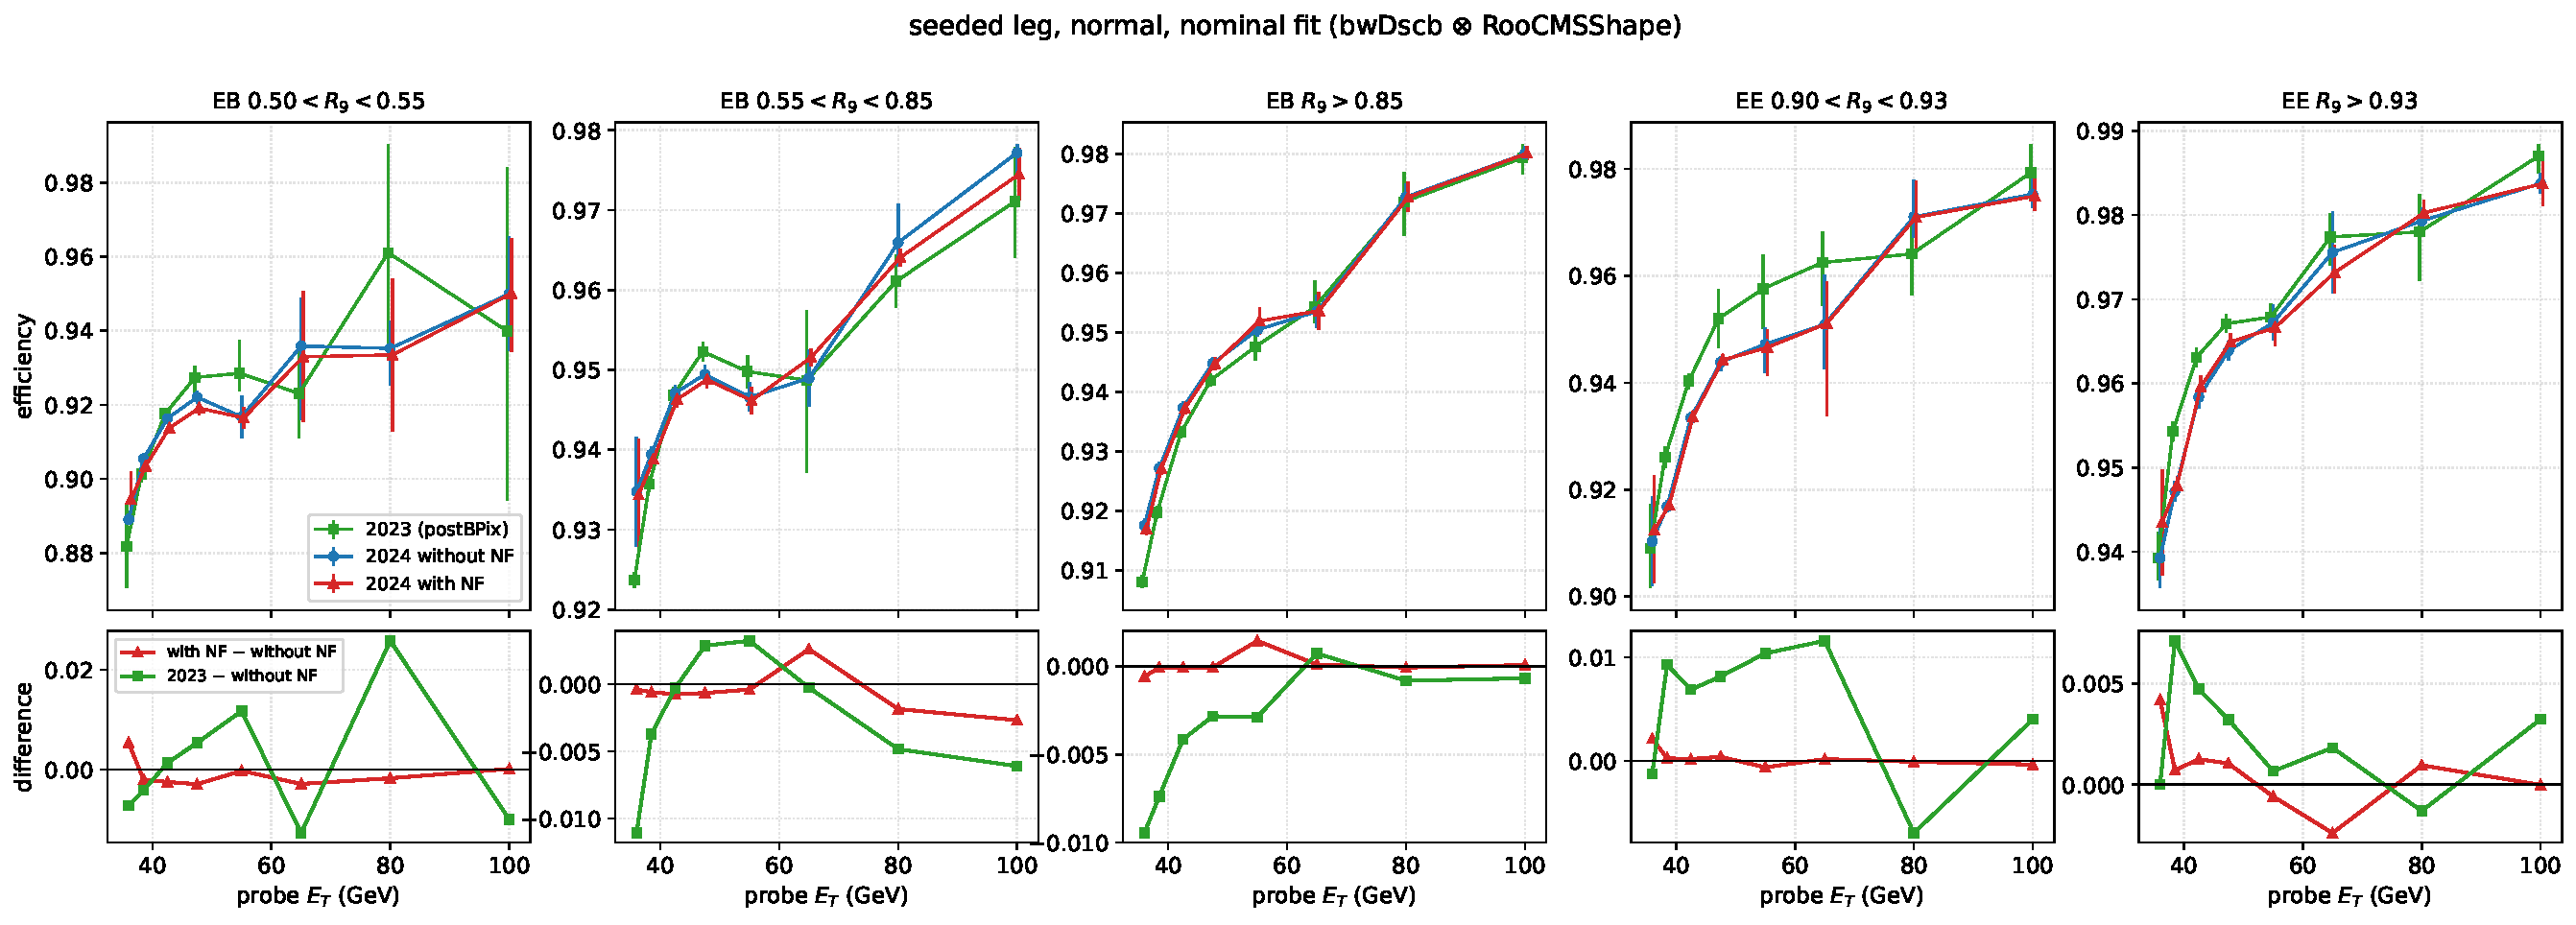
\includegraphics[width=0.98\linewidth,height=0.38\textheight,keepaspectratio]{eff/overview_normal_seed.pdf}}\\[2pt]
  \colorbox{white}{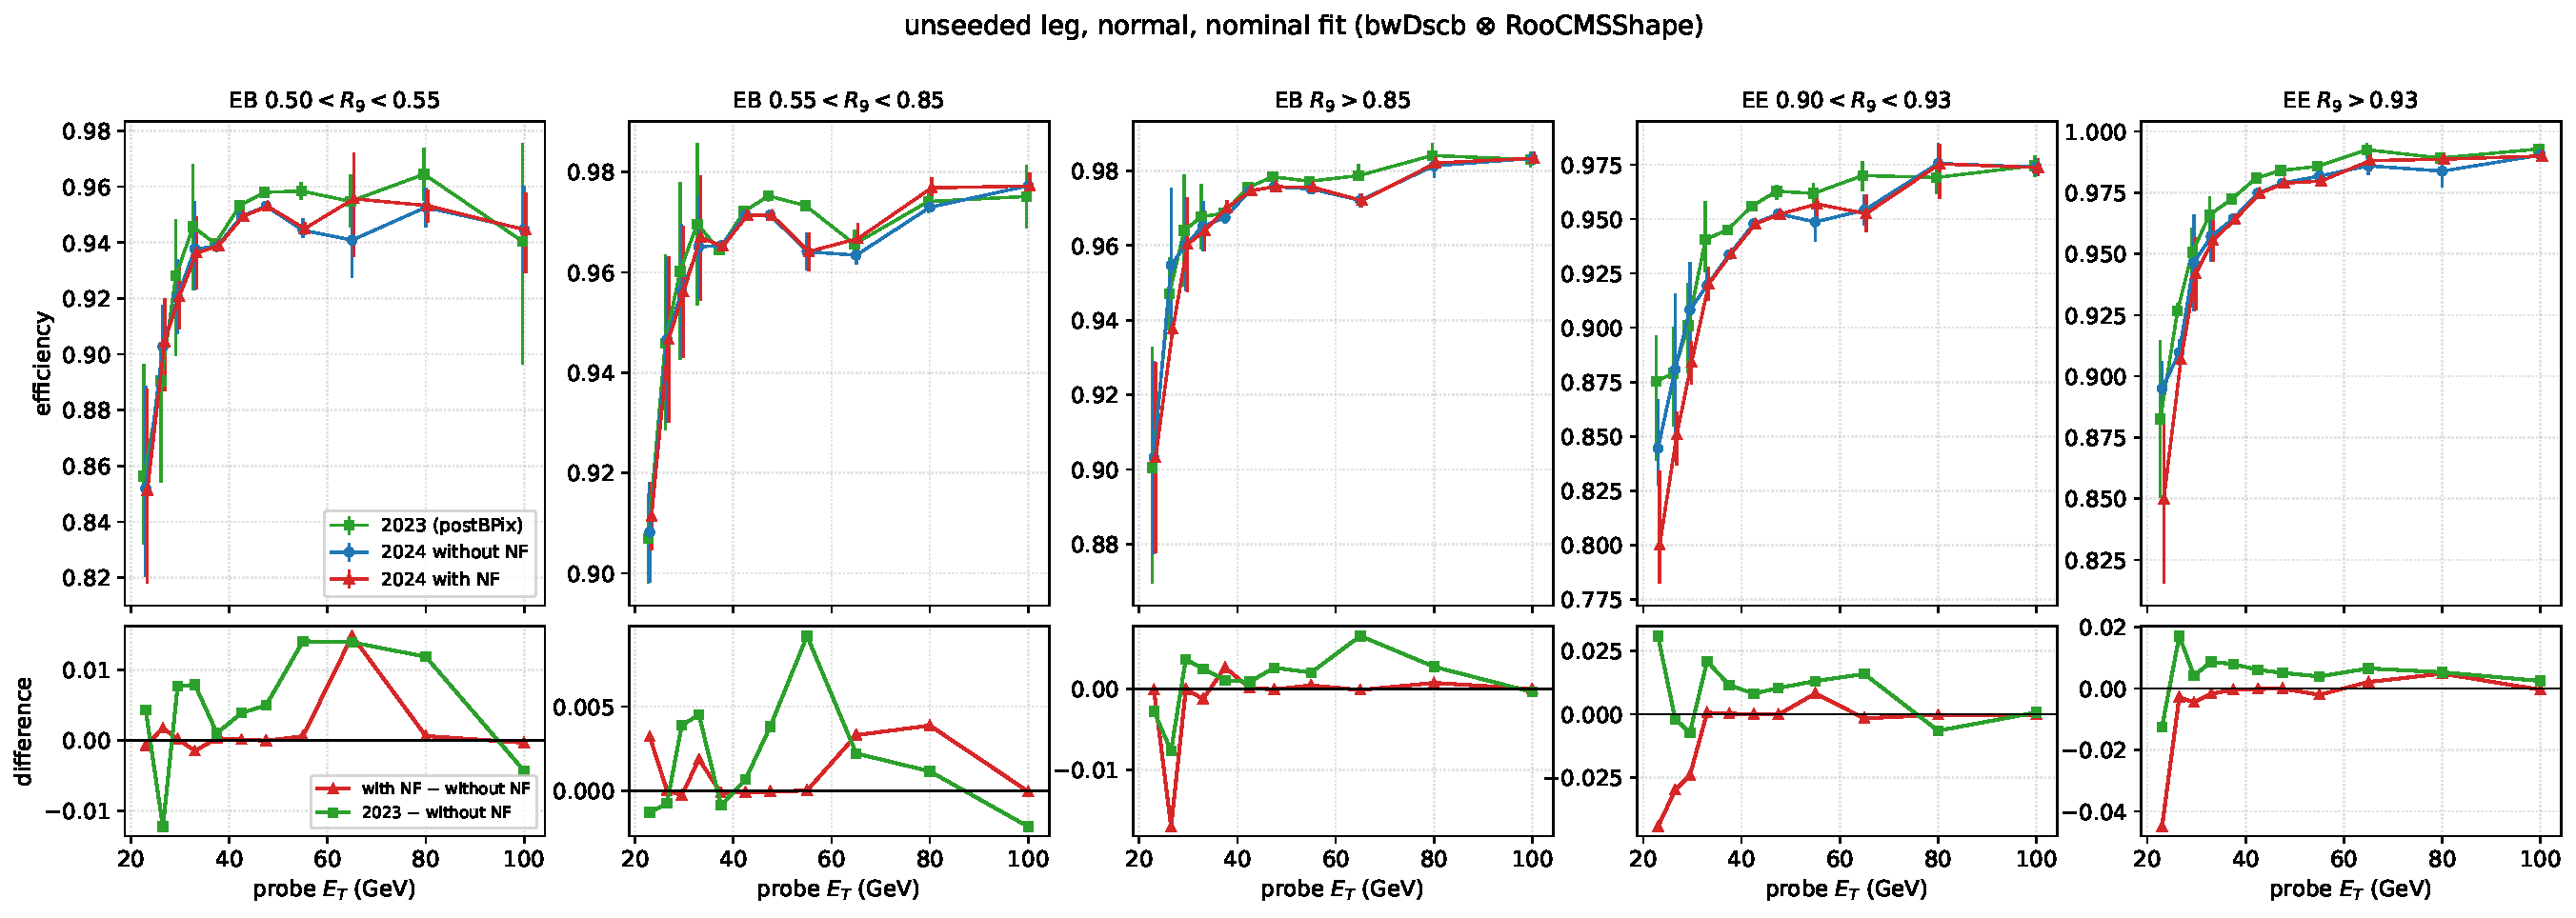
\includegraphics[width=0.98\linewidth,height=0.38\textheight,keepaspectratio]{eff/overview_normal_unseed.pdf}}
\end{frame}

\begin{frame}{Backup: fitted vs counting shift --- seeded, and fullPath}
  \centering
  \wimg{0.98\linewidth}{why/fit_vs_count_vs_pt_normal_seed.pdf}\\[2pt]
  \wimg{0.98\linewidth}{why/fit_vs_count_vs_pt_fullPath_unseed.pdf}\\[2pt]
  {\tiny\color{lightgrey} Top: seeded, normal. Bottom: unseeded, fullPath.}
\end{frame}

\begin{frame}{Backup: mean weight of passing vs failing probes --- seeded}
  \plotslide[0.98]{why/wpass_over_wfail_seed.pdf}{}
\end{frame}

\begin{frame}{Backup: fit pairs for shifts 2--4}
  \centering
  \colorbox{white}{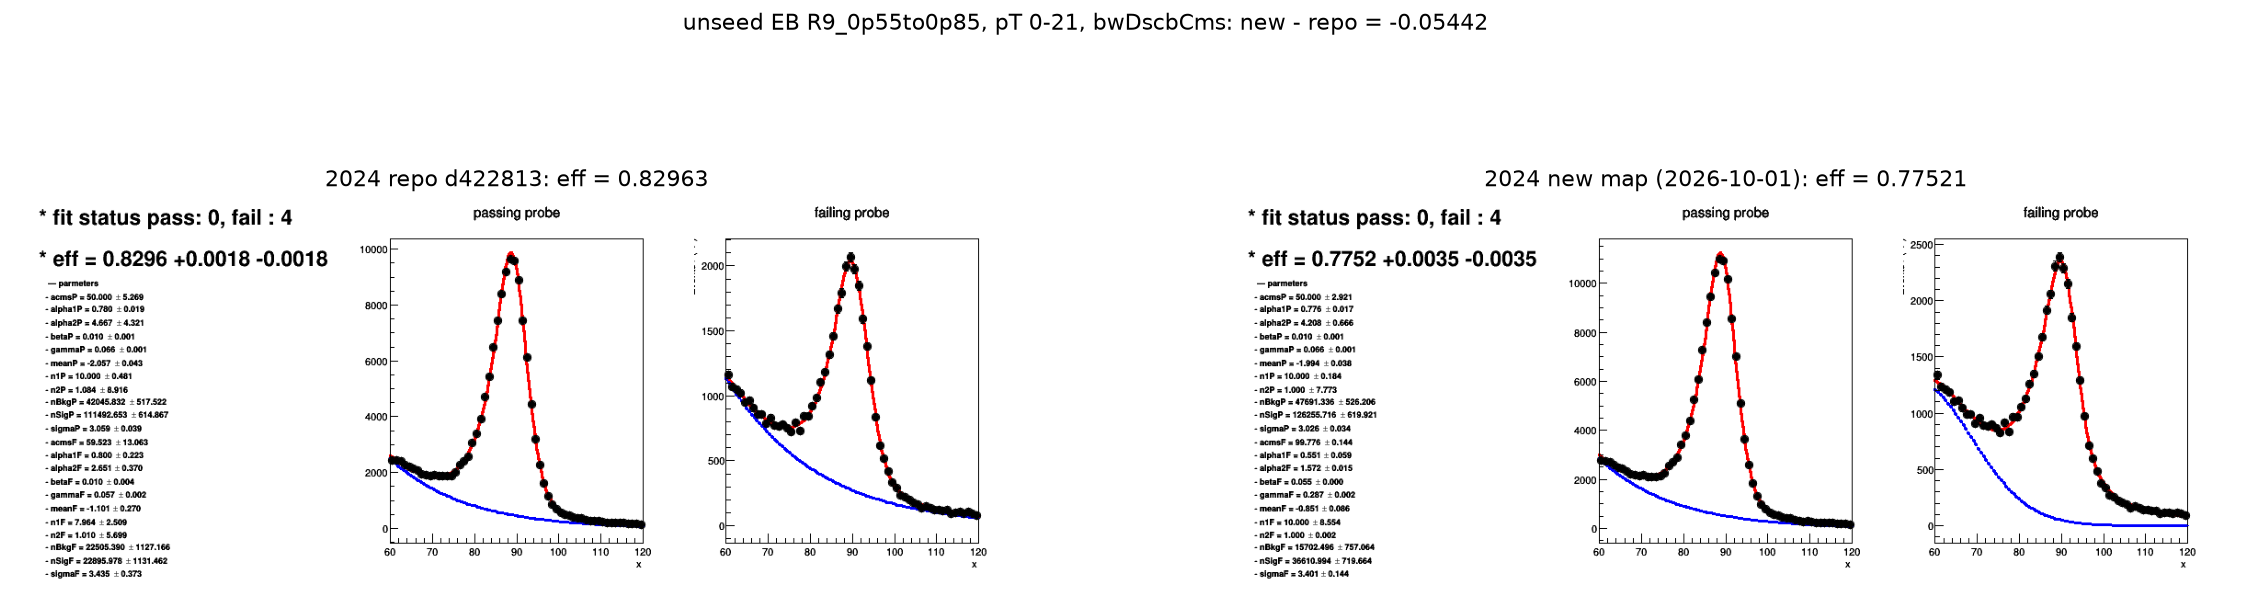
\includegraphics[width=0.85\linewidth,height=0.22\textheight,keepaspectratio]{why/fit_shift3_unseed_EB_R9_0p55to0p85_0_bwDscbCms.png}}\\[2pt]
  \colorbox{white}{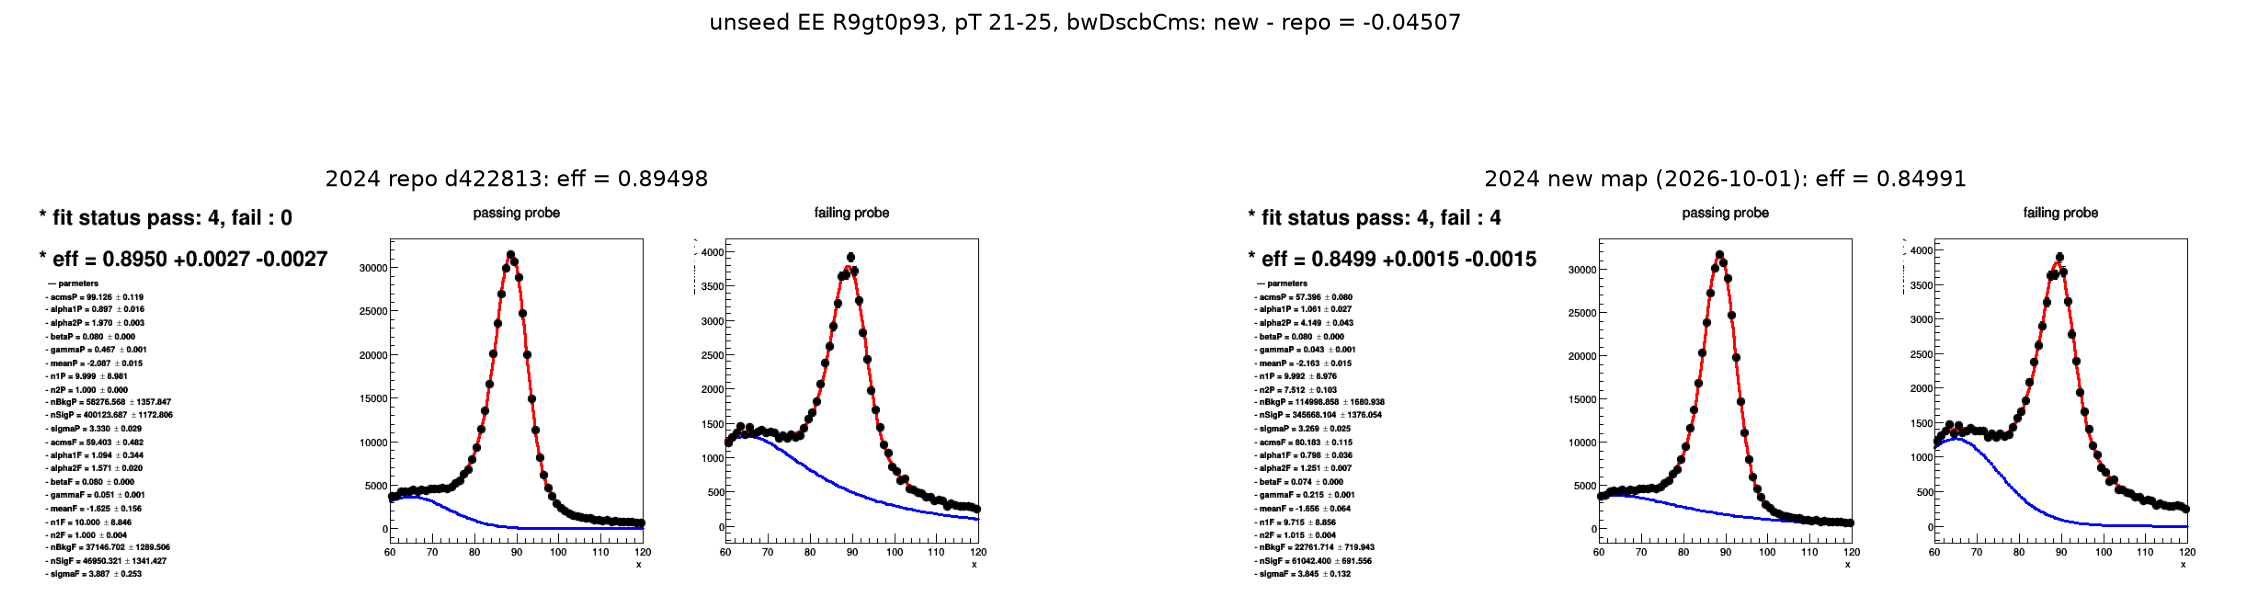
\includegraphics[width=0.85\linewidth,height=0.22\textheight,keepaspectratio]{why/fit_shift4_unseed_EE_R9gt0p93_21_bwDscbCms.png}}\\[2pt]
  \colorbox{white}{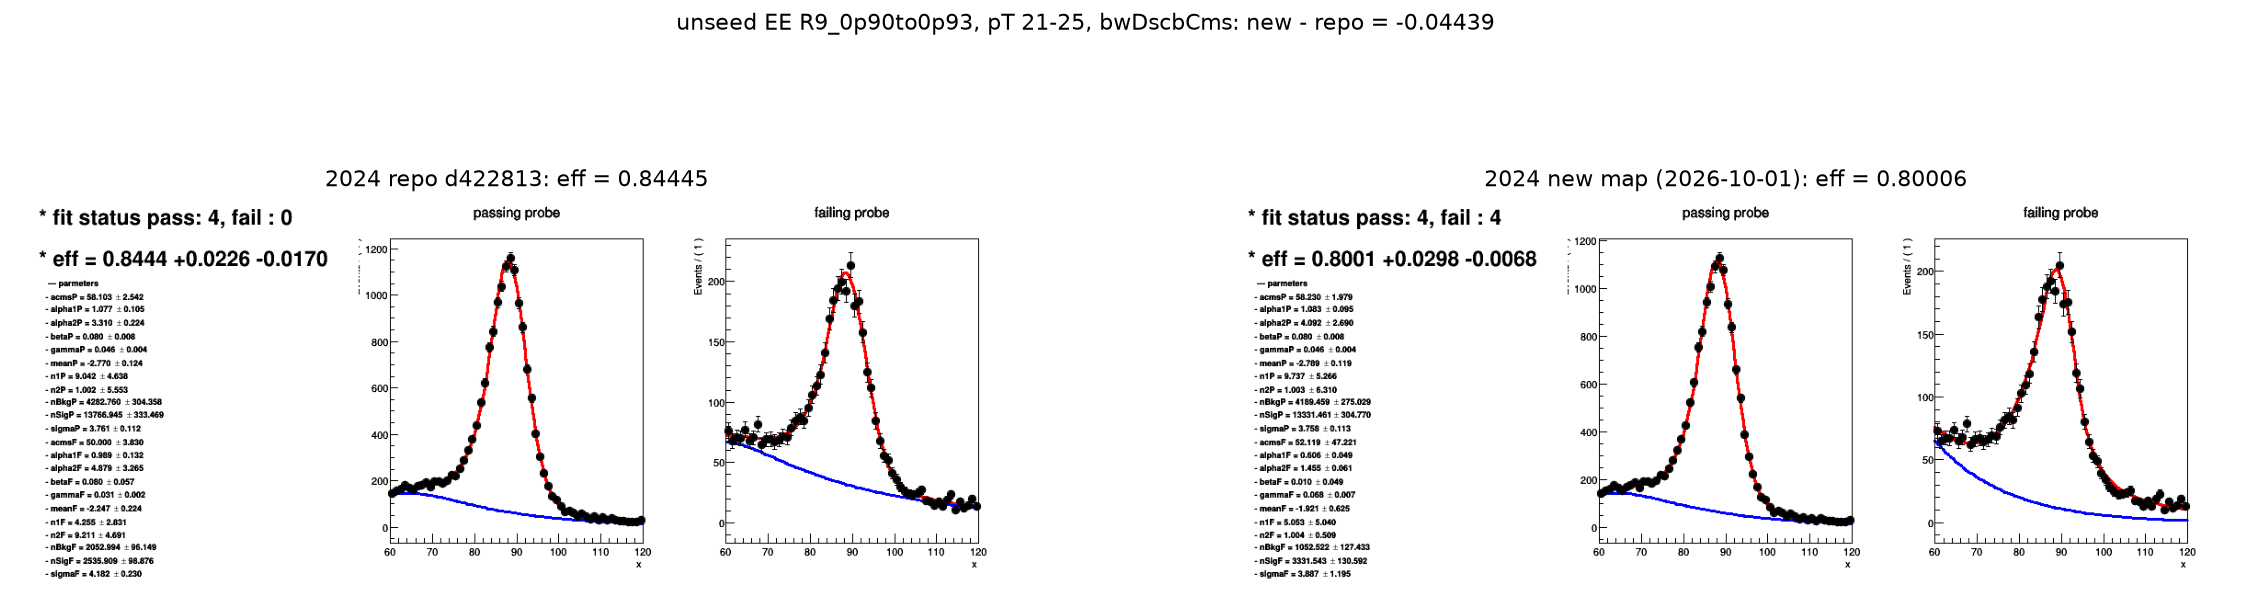
\includegraphics[width=0.85\linewidth,height=0.22\textheight,keepaspectratio]{why/fit_shift5_unseed_EE_R9_0p90to0p93_21_bwDscbCms.png}}\\[2pt]
  {\tiny\color{lightgrey} Left without NF, right with NF. Unseeded EB $0.55<\RNine<0.85$ 0--21; EE $\RNine>0.93$ 21--25; EE $0.90<\RNine<0.93$ 21--25 (nominal fit).}
\end{frame}

\begin{frame}{Backup: size of the map change vs size of the fitted shift}
  \plotslide[0.98]{why/chain_map_change_vs_fit_shift.pdf}
    {Per fitter bin. $m_{\rm pass}$, $m_{\rm fail}$: weighted yield with NF / without NF. Right: spread of the per-cell weight ratio over the failing probes.}
  \vspace{-4pt}
  {\scriptsize Spearman correlation with $|$fitted shift$|$, normal set: 0.46, 0.03, 0.26 (left to right); fullPath: 0.53, 0.32, 0.24.}
\end{frame}

\begin{frame}{Backup: histogram totals vs fitted signal yields --- seeded}
  \plotslide[0.98]{why/chain_yield_ratio_vs_pt_seed.pdf}{Same layout as the unseeded slide.}
\end{frame}

% generated by diagnostics/2026-10-05_add_fit_frames.py

\begin{frame}[label=fit-seed-EB-R9-0p50to0p55-0]{Fits: seeded leg, EB $0.50<\RNine<0.55$, $0<\ET<35$~GeV}
  \centering
  {\scriptsize\hl{without NF}}\\[1pt]
  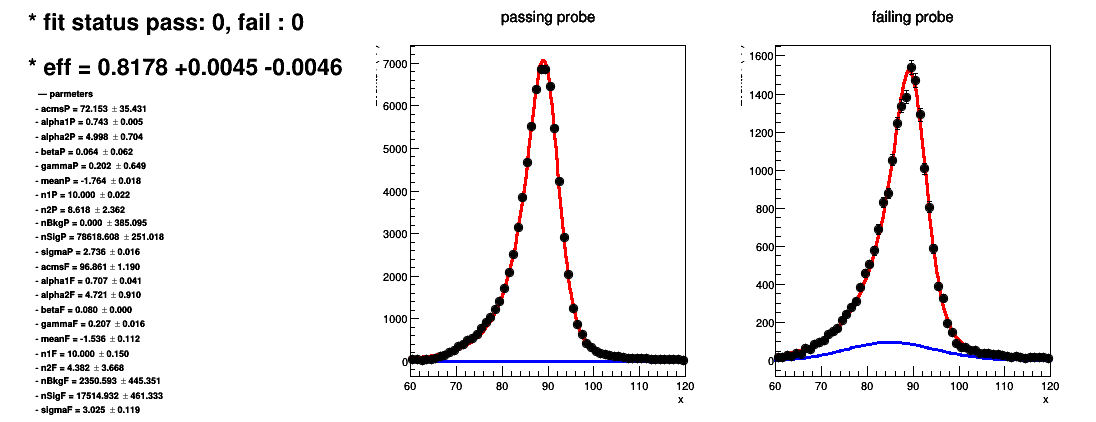
\includegraphics[height=0.355\textheight]{fits/woNF/seed_EB_R9_0p50to0p55_et0.png}\\[2pt]
  {\scriptsize\hl{with NF}}\\[1pt]
  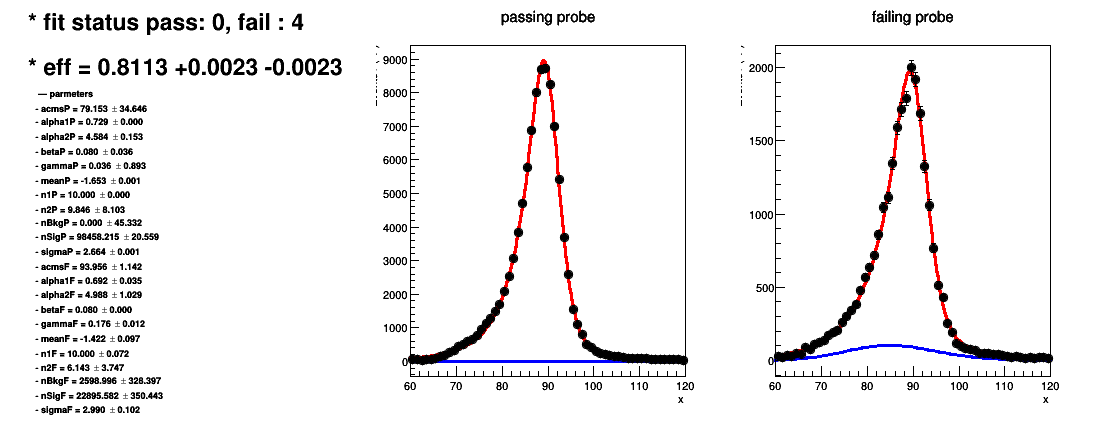
\includegraphics[height=0.355\textheight]{fits/wNF/seed_EB_R9_0p50to0p55_et0.png}\\[2pt]
  \vspace{-10pt}\hfill\hyperlink{eff-seed-EB}{\beamerreturnbutton{efficiency}}
\end{frame}

\begin{frame}[label=fit-seed-EB-R9-0p50to0p55-35]{Fits: seeded leg, EB $0.50<\RNine<0.55$, $35<\ET<37$~GeV}
  \centering
  {\scriptsize\hl{without NF}}\\[1pt]
  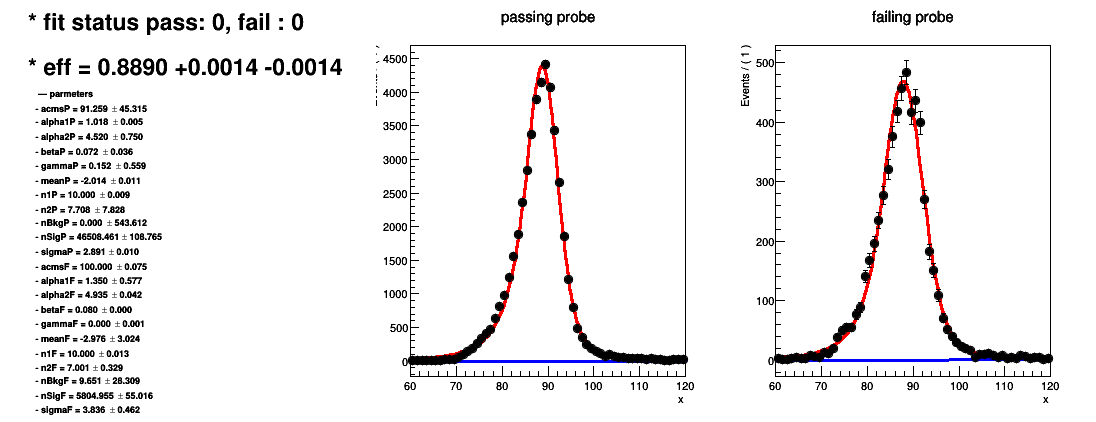
\includegraphics[height=0.355\textheight]{fits/woNF/seed_EB_R9_0p50to0p55_et35.png}\\[2pt]
  {\scriptsize\hl{with NF}}\\[1pt]
  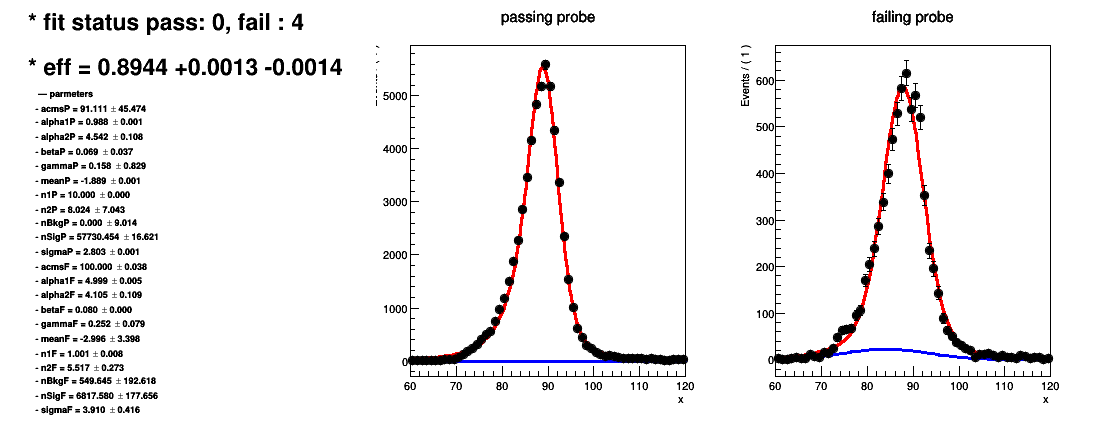
\includegraphics[height=0.355\textheight]{fits/wNF/seed_EB_R9_0p50to0p55_et35.png}\\[2pt]
  \vspace{-10pt}\hfill\hyperlink{eff-seed-EB}{\beamerreturnbutton{efficiency}}
\end{frame}

\begin{frame}[label=fit-seed-EB-R9-0p50to0p55-37]{Fits: seeded leg, EB $0.50<\RNine<0.55$, $37<\ET<40$~GeV}
  \centering
  {\scriptsize\hl{without NF}}\\[1pt]
  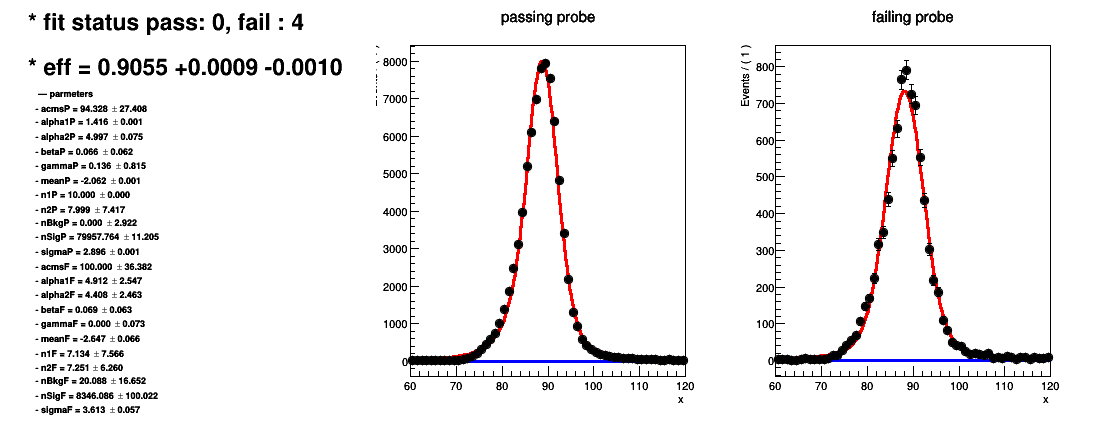
\includegraphics[height=0.355\textheight]{fits/woNF/seed_EB_R9_0p50to0p55_et37.png}\\[2pt]
  {\scriptsize\hl{with NF}}\\[1pt]
  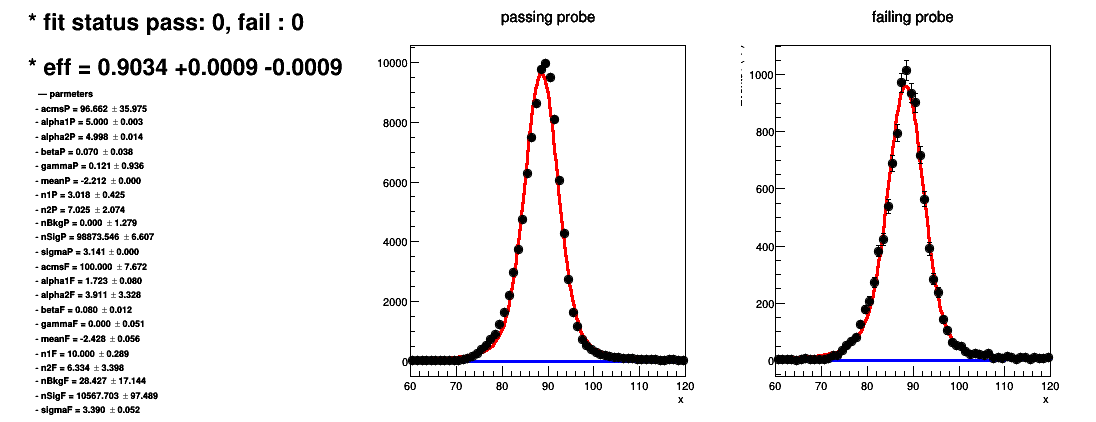
\includegraphics[height=0.355\textheight]{fits/wNF/seed_EB_R9_0p50to0p55_et37.png}\\[2pt]
  \vspace{-10pt}\hfill\hyperlink{eff-seed-EB}{\beamerreturnbutton{efficiency}}
\end{frame}

\begin{frame}[label=fit-seed-EB-R9-0p50to0p55-40]{Fits: seeded leg, EB $0.50<\RNine<0.55$, $40<\ET<45$~GeV}
  \centering
  {\scriptsize\hl{without NF}}\\[1pt]
  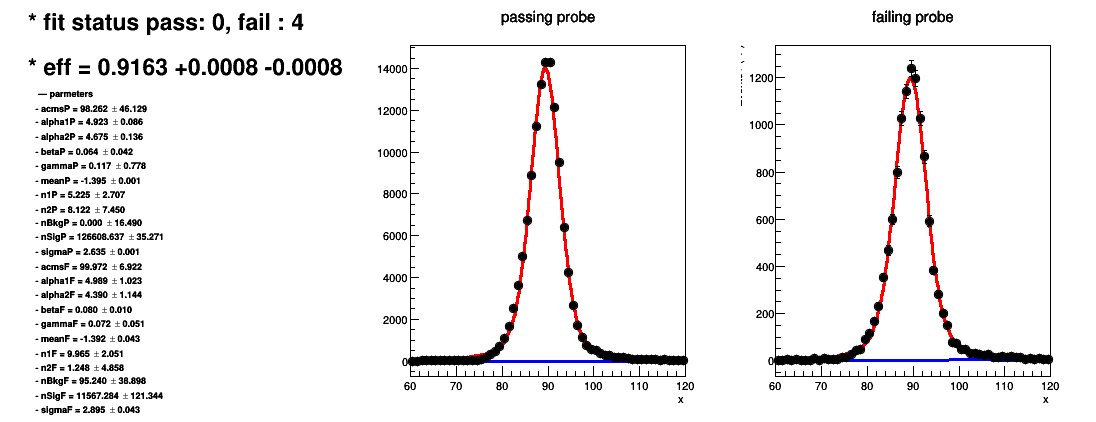
\includegraphics[height=0.355\textheight]{fits/woNF/seed_EB_R9_0p50to0p55_et40.png}\\[2pt]
  {\scriptsize\hl{with NF}}\\[1pt]
  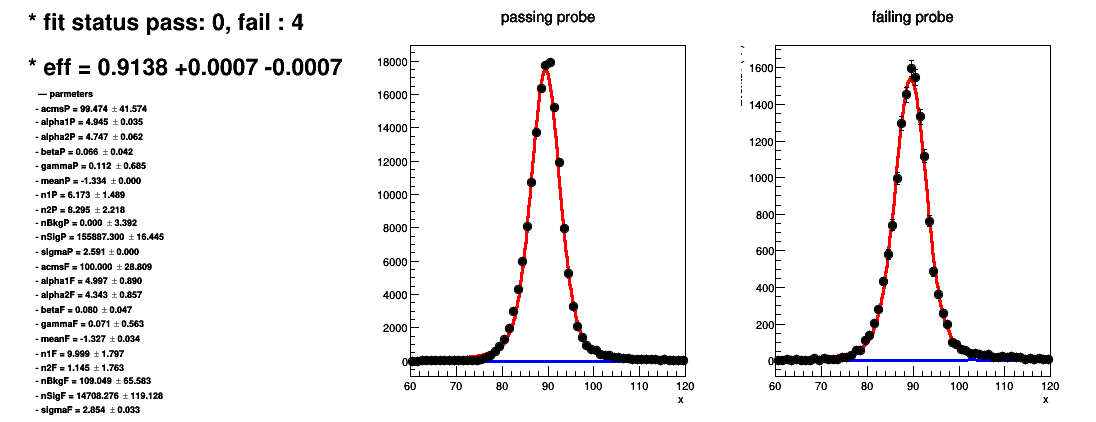
\includegraphics[height=0.355\textheight]{fits/wNF/seed_EB_R9_0p50to0p55_et40.png}\\[2pt]
  \vspace{-10pt}\hfill\hyperlink{eff-seed-EB}{\beamerreturnbutton{efficiency}}
\end{frame}

\begin{frame}[label=fit-seed-EB-R9-0p50to0p55-45]{Fits: seeded leg, EB $0.50<\RNine<0.55$, $45<\ET<50$~GeV}
  \centering
  {\scriptsize\hl{without NF}}\\[1pt]
  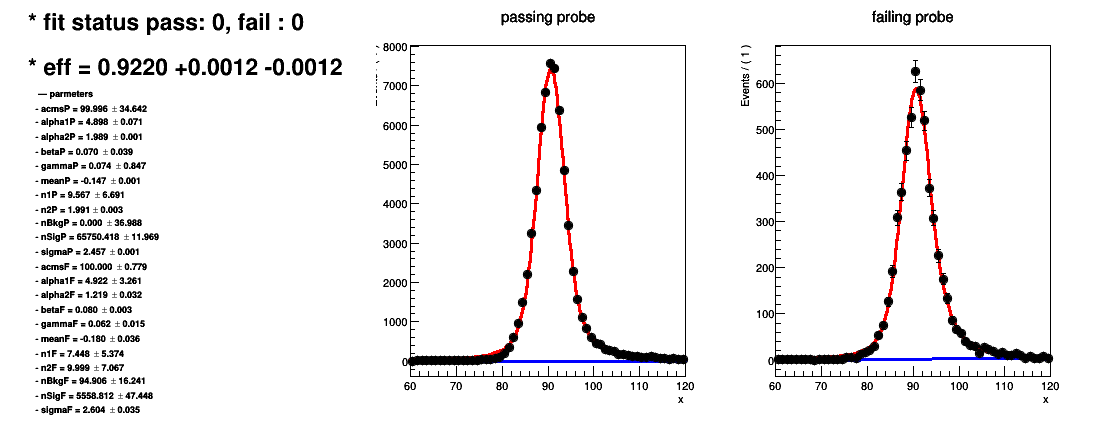
\includegraphics[height=0.355\textheight]{fits/woNF/seed_EB_R9_0p50to0p55_et45.png}\\[2pt]
  {\scriptsize\hl{with NF}}\\[1pt]
  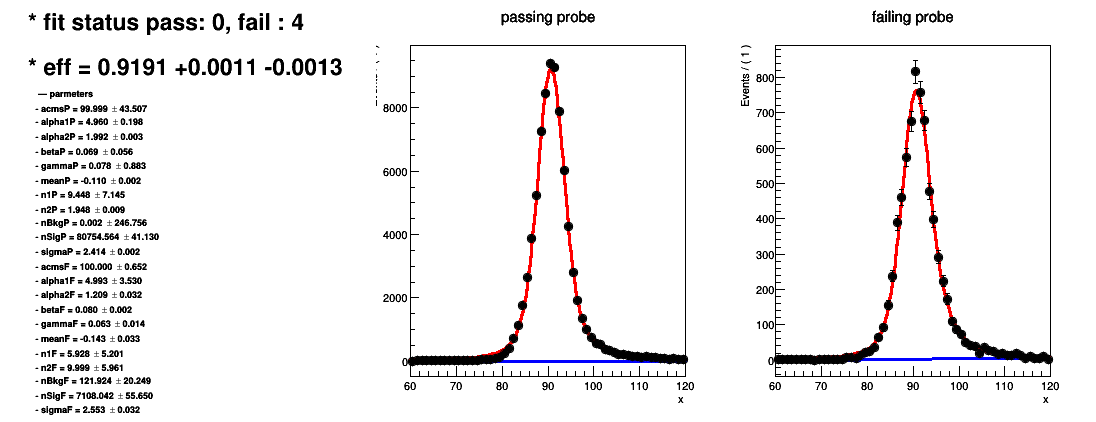
\includegraphics[height=0.355\textheight]{fits/wNF/seed_EB_R9_0p50to0p55_et45.png}\\[2pt]
  \vspace{-10pt}\hfill\hyperlink{eff-seed-EB}{\beamerreturnbutton{efficiency}}
\end{frame}

\begin{frame}[label=fit-seed-EB-R9-0p50to0p55-50]{Fits: seeded leg, EB $0.50<\RNine<0.55$, $50<\ET<60$~GeV}
  \centering
  {\scriptsize\hl{without NF}}\\[1pt]
  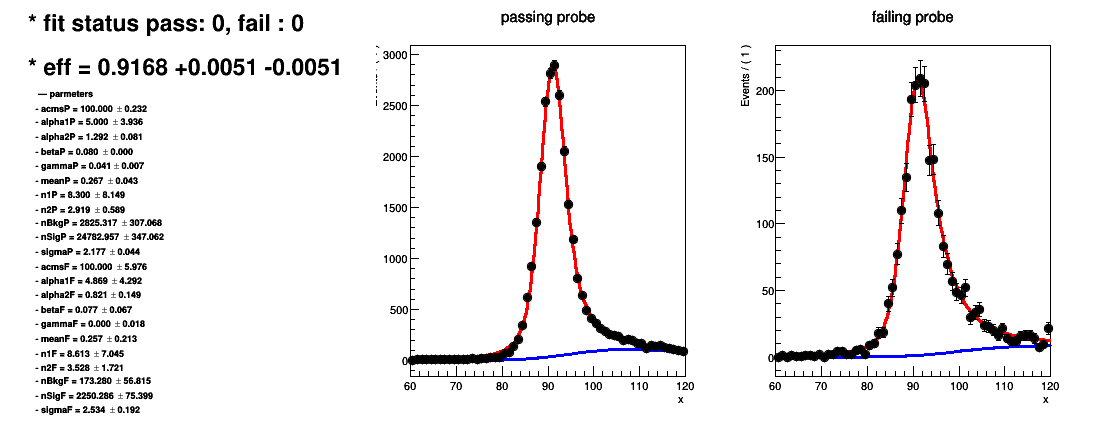
\includegraphics[height=0.355\textheight]{fits/woNF/seed_EB_R9_0p50to0p55_et50.png}\\[2pt]
  {\scriptsize\hl{with NF}}\\[1pt]
  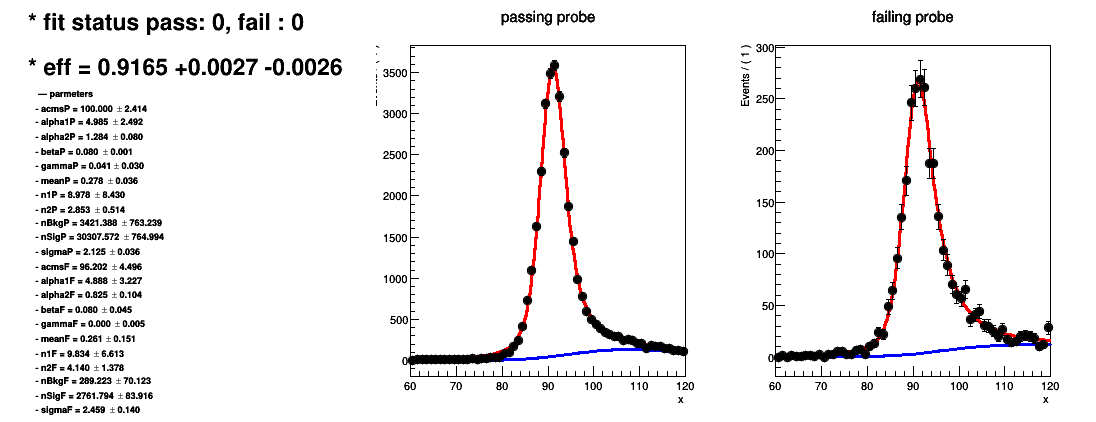
\includegraphics[height=0.355\textheight]{fits/wNF/seed_EB_R9_0p50to0p55_et50.png}\\[2pt]
  \vspace{-10pt}\hfill\hyperlink{eff-seed-EB}{\beamerreturnbutton{efficiency}}
\end{frame}

\begin{frame}[label=fit-seed-EB-R9-0p50to0p55-60]{Fits: seeded leg, EB $0.50<\RNine<0.55$, $60<\ET<70$~GeV}
  \centering
  {\scriptsize\hl{without NF}}\\[1pt]
  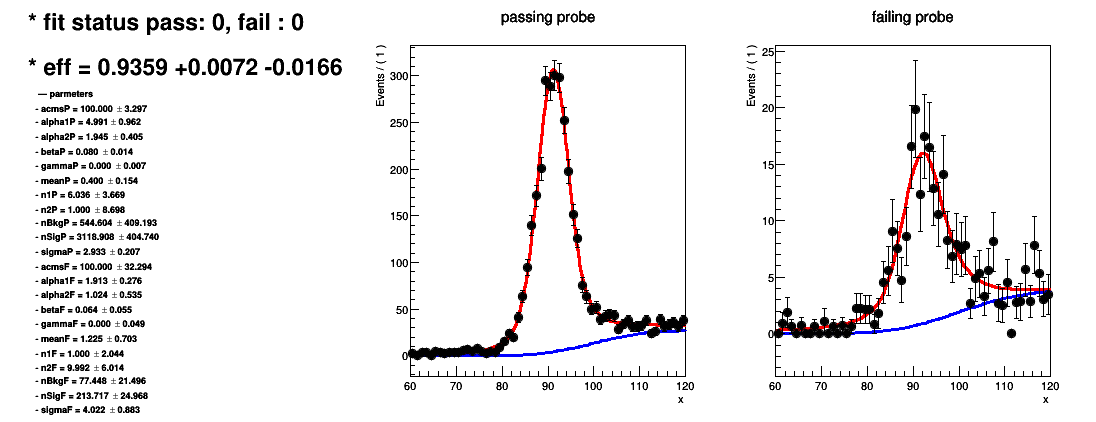
\includegraphics[height=0.355\textheight]{fits/woNF/seed_EB_R9_0p50to0p55_et60.png}\\[2pt]
  {\scriptsize\hl{with NF}}\\[1pt]
  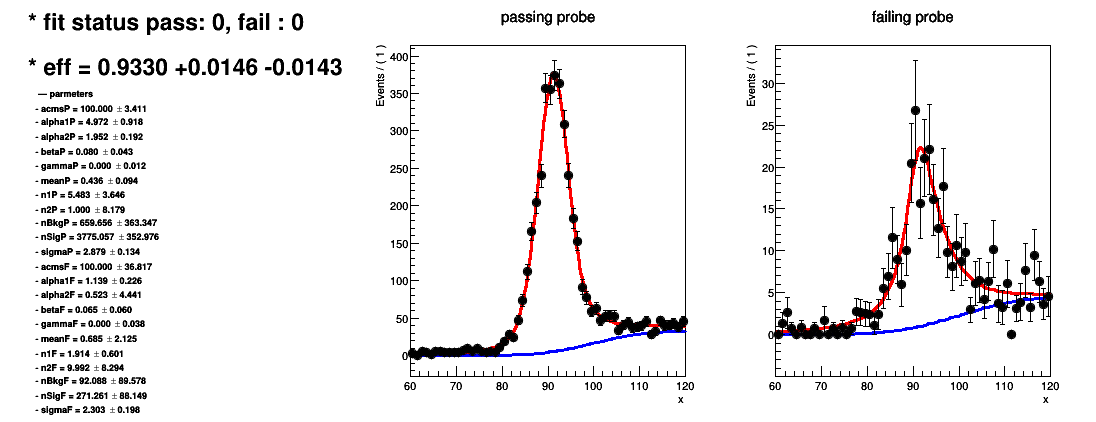
\includegraphics[height=0.355\textheight]{fits/wNF/seed_EB_R9_0p50to0p55_et60.png}\\[2pt]
  \vspace{-10pt}\hfill\hyperlink{eff-seed-EB}{\beamerreturnbutton{efficiency}}
\end{frame}

\begin{frame}[label=fit-seed-EB-R9-0p50to0p55-70]{Fits: seeded leg, EB $0.50<\RNine<0.55$, $70<\ET<90$~GeV}
  \centering
  {\scriptsize\hl{without NF}}\\[1pt]
  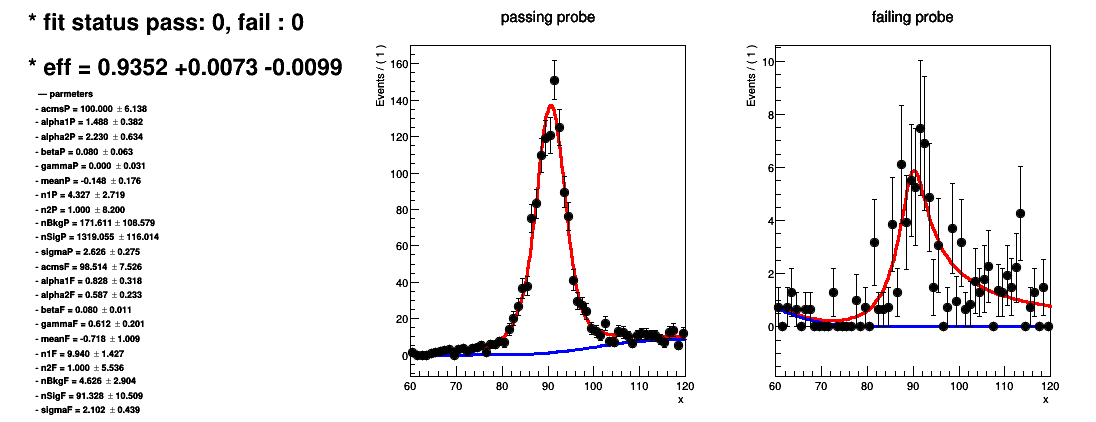
\includegraphics[height=0.355\textheight]{fits/woNF/seed_EB_R9_0p50to0p55_et70.png}\\[2pt]
  {\scriptsize\hl{with NF}}\\[1pt]
  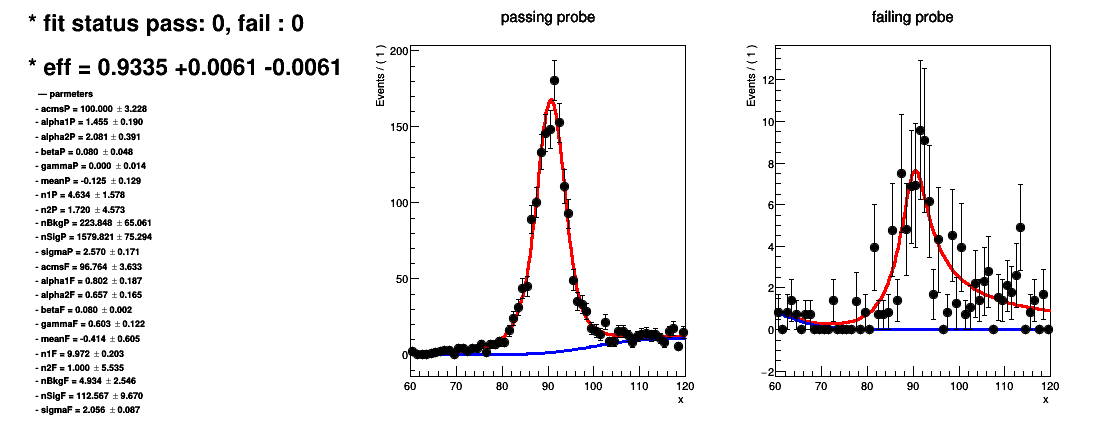
\includegraphics[height=0.355\textheight]{fits/wNF/seed_EB_R9_0p50to0p55_et70.png}\\[2pt]
  \vspace{-10pt}\hfill\hyperlink{eff-seed-EB}{\beamerreturnbutton{efficiency}}
\end{frame}

\begin{frame}[label=fit-seed-EB-R9-0p50to0p55-90]{Fits: seeded leg, EB $0.50<\RNine<0.55$, $\ET>90$~GeV}
  \centering
  {\scriptsize\hl{without NF}}\\[1pt]
  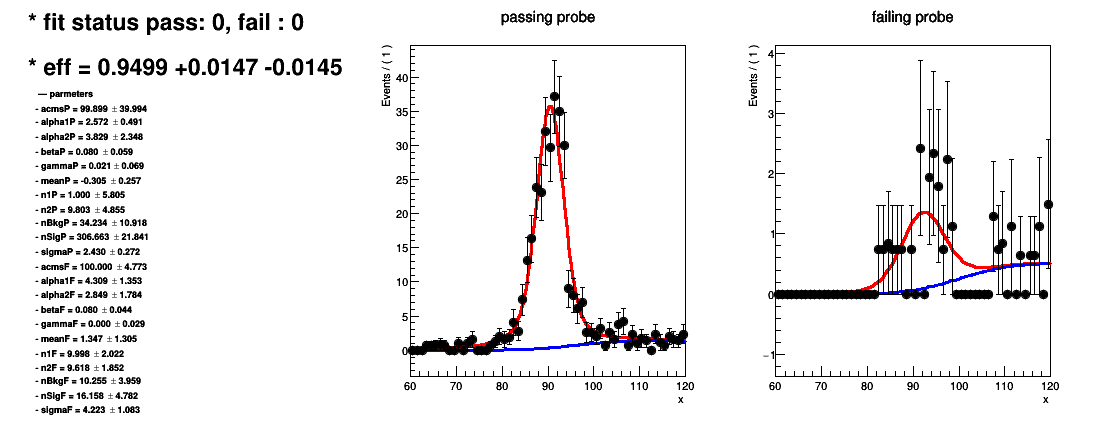
\includegraphics[height=0.355\textheight]{fits/woNF/seed_EB_R9_0p50to0p55_et90.png}\\[2pt]
  {\scriptsize\hl{with NF}}\\[1pt]
  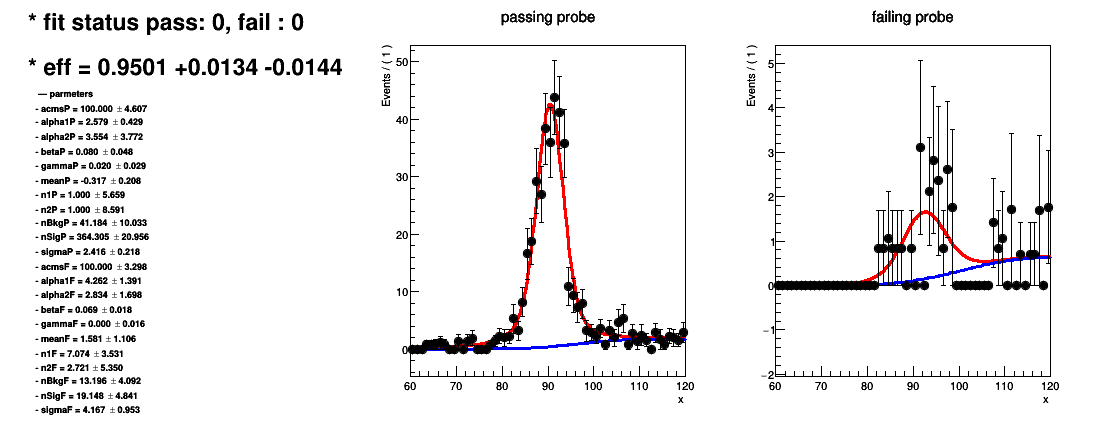
\includegraphics[height=0.355\textheight]{fits/wNF/seed_EB_R9_0p50to0p55_et90.png}\\[2pt]
  \vspace{-10pt}\hfill\hyperlink{eff-seed-EB}{\beamerreturnbutton{efficiency}}
\end{frame}

\begin{frame}[label=fit-seed-EB-R9-0p55to0p85-0]{Fits: seeded leg, EB $0.55<\RNine<0.85$, $0<\ET<35$~GeV}
  \centering
  {\scriptsize\hl{without NF}}\\[1pt]
  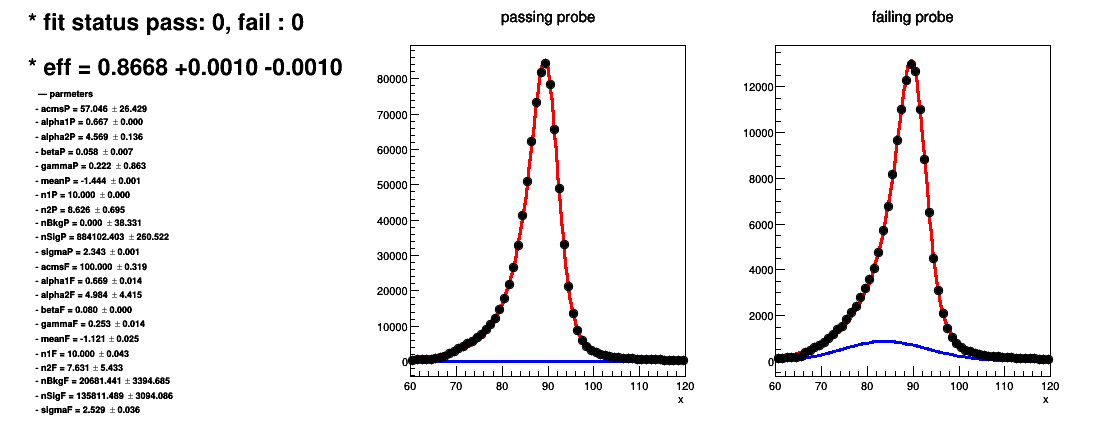
\includegraphics[height=0.355\textheight]{fits/woNF/seed_EB_R9_0p55to0p85_et0.png}\\[2pt]
  {\scriptsize\hl{with NF}}\\[1pt]
  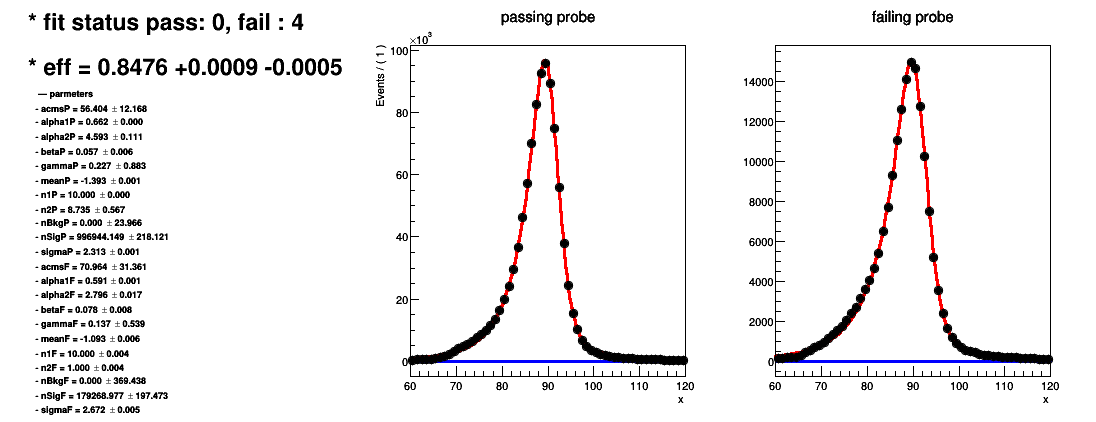
\includegraphics[height=0.355\textheight]{fits/wNF/seed_EB_R9_0p55to0p85_et0.png}\\[2pt]
  \vspace{-10pt}\hfill\hyperlink{eff-seed-EB}{\beamerreturnbutton{efficiency}}
\end{frame}

\begin{frame}[label=fit-seed-EB-R9-0p55to0p85-35]{Fits: seeded leg, EB $0.55<\RNine<0.85$, $35<\ET<37$~GeV}
  \centering
  {\scriptsize\hl{without NF}}\\[1pt]
  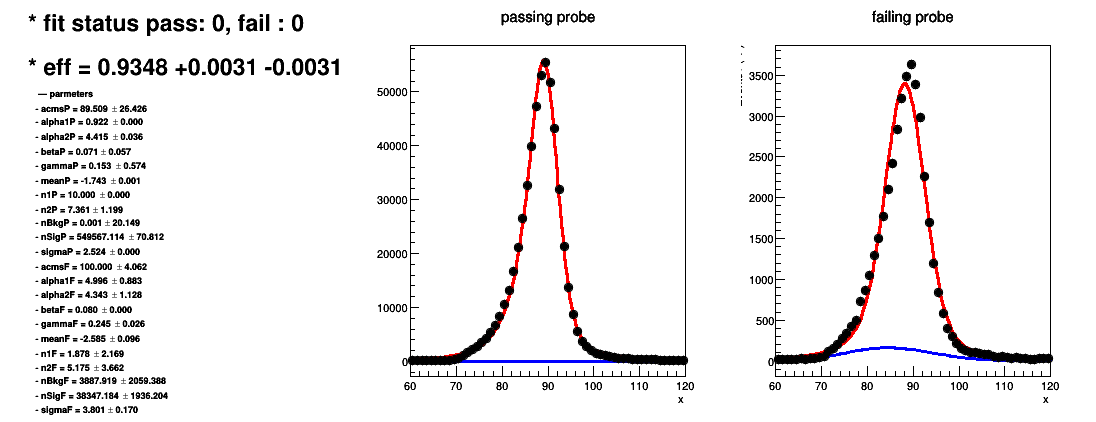
\includegraphics[height=0.355\textheight]{fits/woNF/seed_EB_R9_0p55to0p85_et35.png}\\[2pt]
  {\scriptsize\hl{with NF}}\\[1pt]
  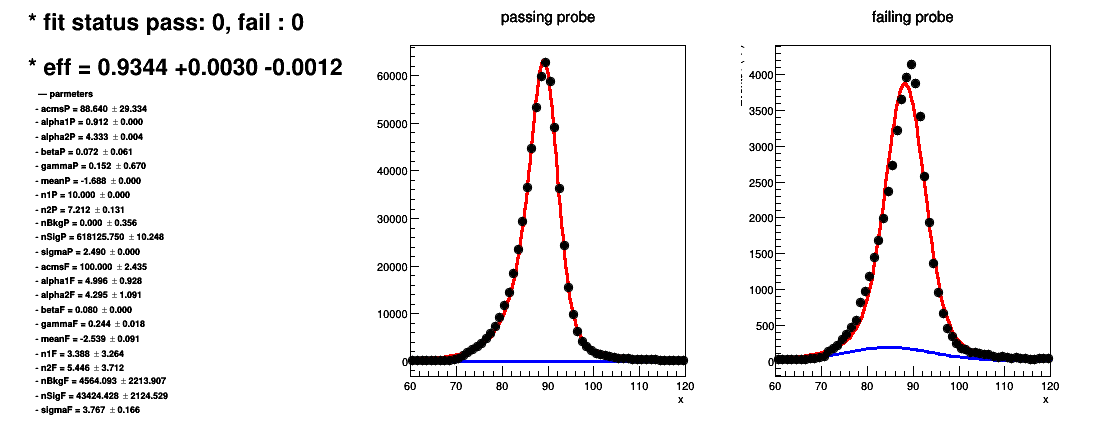
\includegraphics[height=0.355\textheight]{fits/wNF/seed_EB_R9_0p55to0p85_et35.png}\\[2pt]
  \vspace{-10pt}\hfill\hyperlink{eff-seed-EB}{\beamerreturnbutton{efficiency}}
\end{frame}

\begin{frame}[label=fit-seed-EB-R9-0p55to0p85-37]{Fits: seeded leg, EB $0.55<\RNine<0.85$, $37<\ET<40$~GeV}
  \centering
  {\scriptsize\hl{without NF}}\\[1pt]
  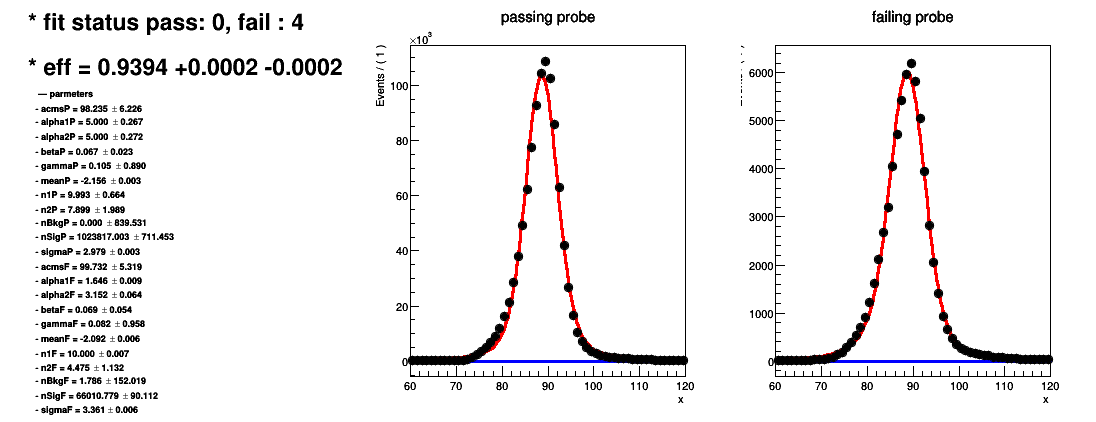
\includegraphics[height=0.355\textheight]{fits/woNF/seed_EB_R9_0p55to0p85_et37.png}\\[2pt]
  {\scriptsize\hl{with NF}}\\[1pt]
  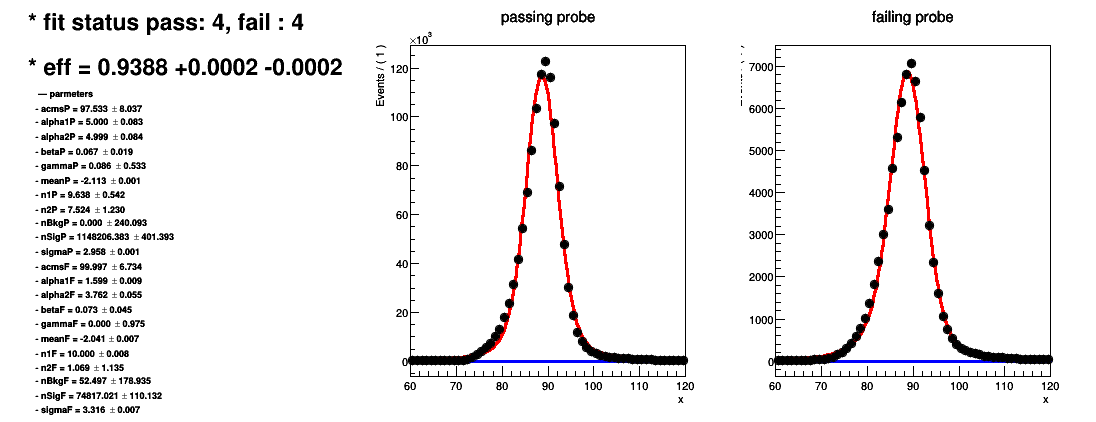
\includegraphics[height=0.355\textheight]{fits/wNF/seed_EB_R9_0p55to0p85_et37.png}\\[2pt]
  \vspace{-10pt}\hfill\hyperlink{eff-seed-EB}{\beamerreturnbutton{efficiency}}
\end{frame}

\begin{frame}[label=fit-seed-EB-R9-0p55to0p85-40]{Fits: seeded leg, EB $0.55<\RNine<0.85$, $40<\ET<45$~GeV}
  \centering
  {\scriptsize\hl{without NF}}\\[1pt]
  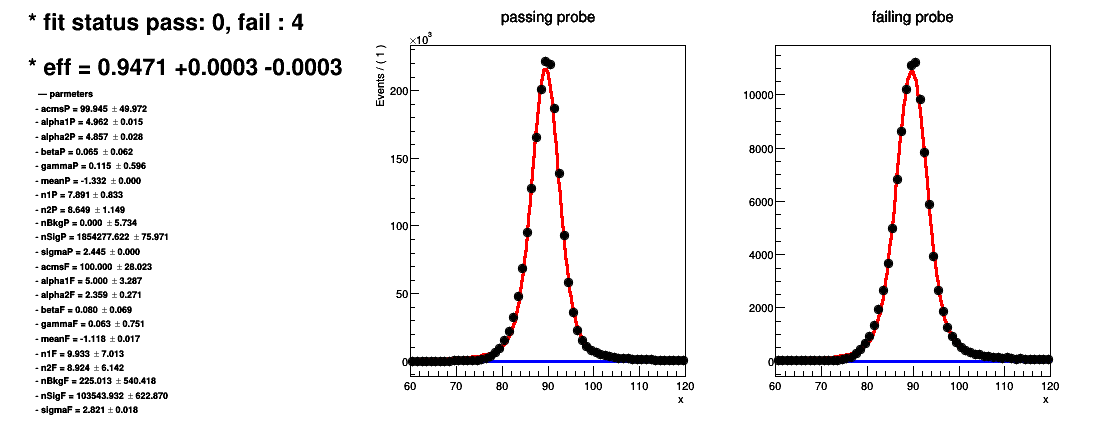
\includegraphics[height=0.355\textheight]{fits/woNF/seed_EB_R9_0p55to0p85_et40.png}\\[2pt]
  {\scriptsize\hl{with NF}}\\[1pt]
  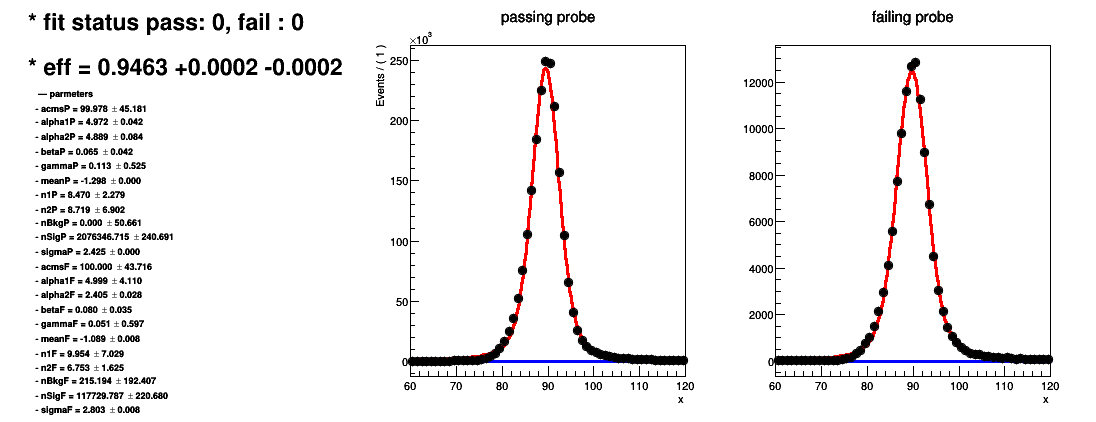
\includegraphics[height=0.355\textheight]{fits/wNF/seed_EB_R9_0p55to0p85_et40.png}\\[2pt]
  \vspace{-10pt}\hfill\hyperlink{eff-seed-EB}{\beamerreturnbutton{efficiency}}
\end{frame}

\begin{frame}[label=fit-seed-EB-R9-0p55to0p85-45]{Fits: seeded leg, EB $0.55<\RNine<0.85$, $45<\ET<50$~GeV}
  \centering
  {\scriptsize\hl{without NF}}\\[1pt]
  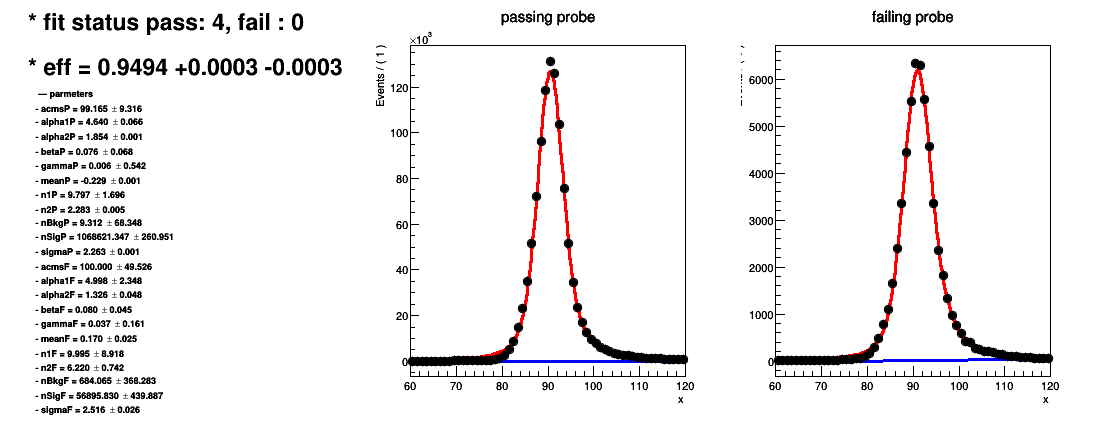
\includegraphics[height=0.355\textheight]{fits/woNF/seed_EB_R9_0p55to0p85_et45.png}\\[2pt]
  {\scriptsize\hl{with NF}}\\[1pt]
  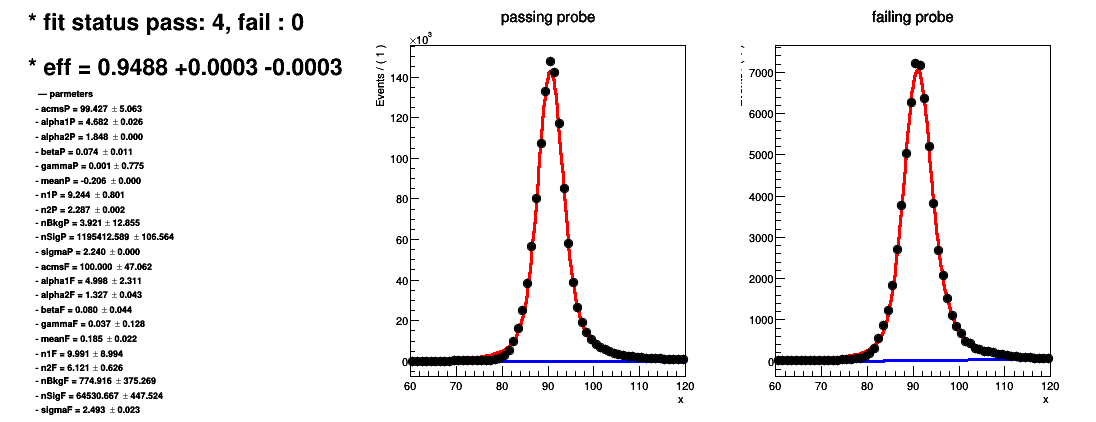
\includegraphics[height=0.355\textheight]{fits/wNF/seed_EB_R9_0p55to0p85_et45.png}\\[2pt]
  \vspace{-10pt}\hfill\hyperlink{eff-seed-EB}{\beamerreturnbutton{efficiency}}
\end{frame}

\begin{frame}[label=fit-seed-EB-R9-0p55to0p85-50]{Fits: seeded leg, EB $0.55<\RNine<0.85$, $50<\ET<60$~GeV}
  \centering
  {\scriptsize\hl{without NF}}\\[1pt]
  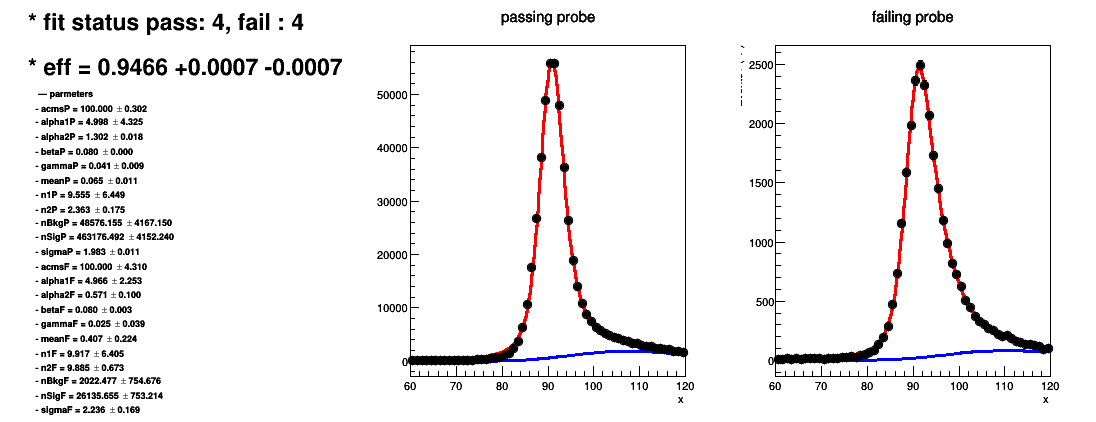
\includegraphics[height=0.355\textheight]{fits/woNF/seed_EB_R9_0p55to0p85_et50.png}\\[2pt]
  {\scriptsize\hl{with NF}}\\[1pt]
  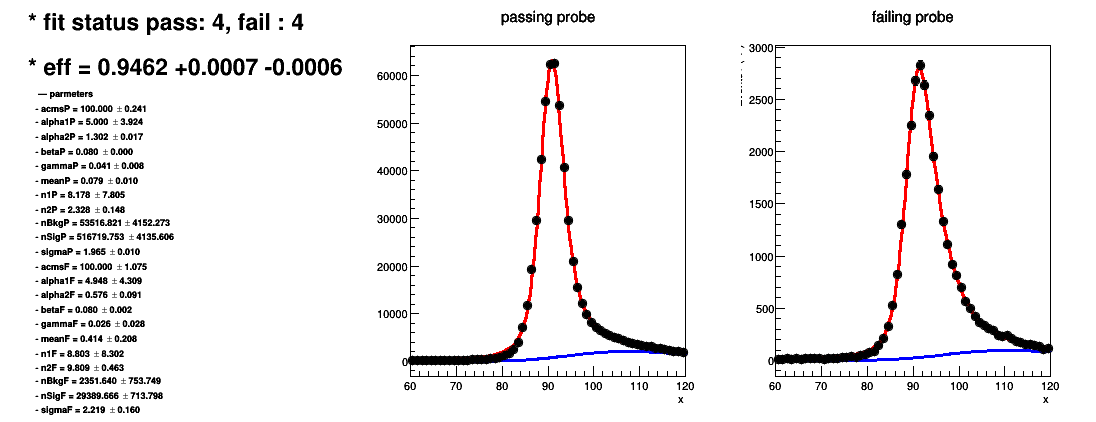
\includegraphics[height=0.355\textheight]{fits/wNF/seed_EB_R9_0p55to0p85_et50.png}\\[2pt]
  \vspace{-10pt}\hfill\hyperlink{eff-seed-EB}{\beamerreturnbutton{efficiency}}
\end{frame}

\begin{frame}[label=fit-seed-EB-R9-0p55to0p85-60]{Fits: seeded leg, EB $0.55<\RNine<0.85$, $60<\ET<70$~GeV}
  \centering
  {\scriptsize\hl{without NF}}\\[1pt]
  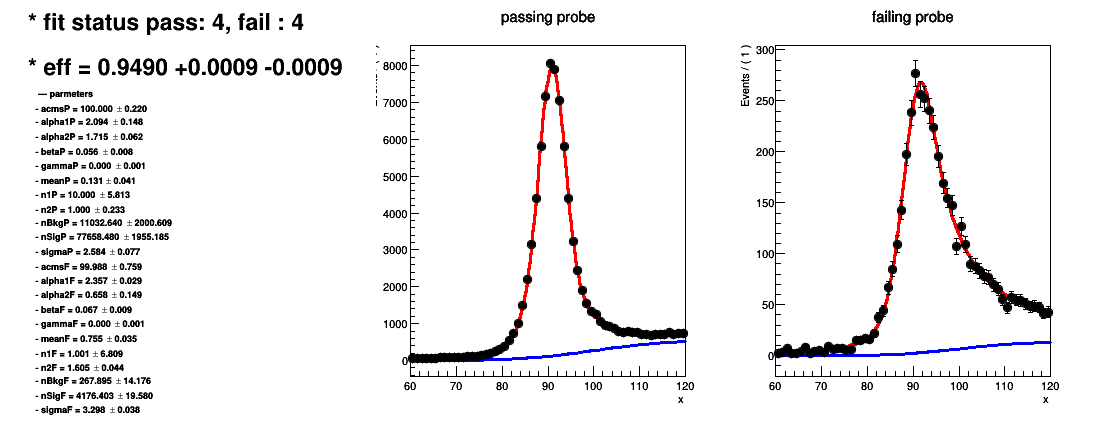
\includegraphics[height=0.355\textheight]{fits/woNF/seed_EB_R9_0p55to0p85_et60.png}\\[2pt]
  {\scriptsize\hl{with NF}}\\[1pt]
  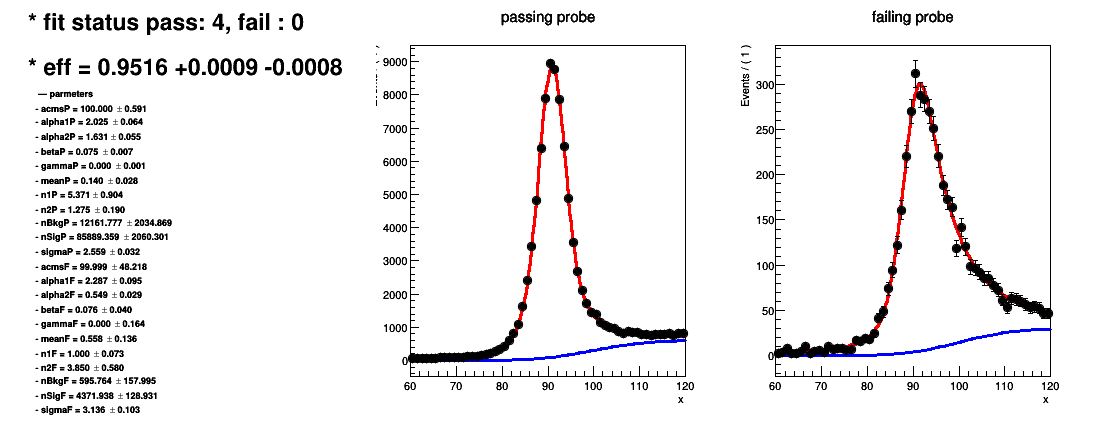
\includegraphics[height=0.355\textheight]{fits/wNF/seed_EB_R9_0p55to0p85_et60.png}\\[2pt]
  \vspace{-10pt}\hfill\hyperlink{eff-seed-EB}{\beamerreturnbutton{efficiency}}
\end{frame}

\begin{frame}[label=fit-seed-EB-R9-0p55to0p85-70]{Fits: seeded leg, EB $0.55<\RNine<0.85$, $70<\ET<90$~GeV}
  \centering
  {\scriptsize\hl{without NF}}\\[1pt]
  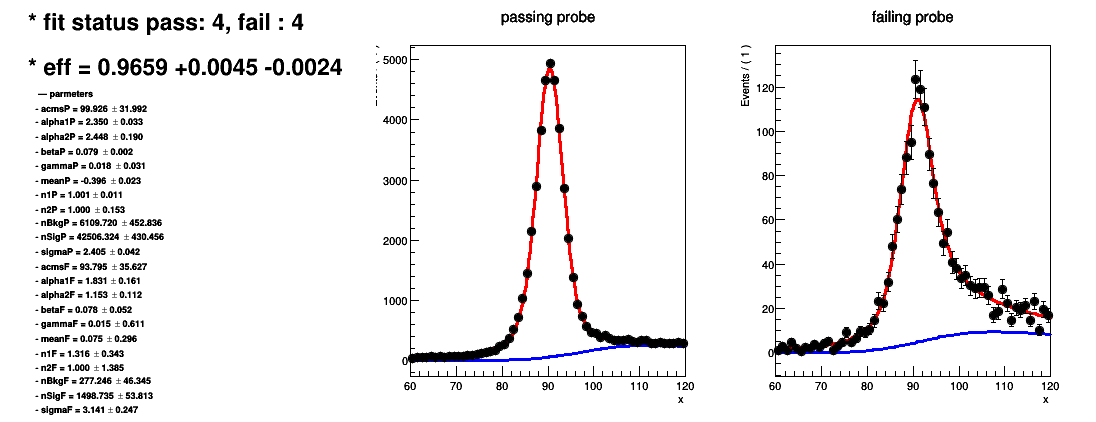
\includegraphics[height=0.355\textheight]{fits/woNF/seed_EB_R9_0p55to0p85_et70.png}\\[2pt]
  {\scriptsize\hl{with NF}}\\[1pt]
  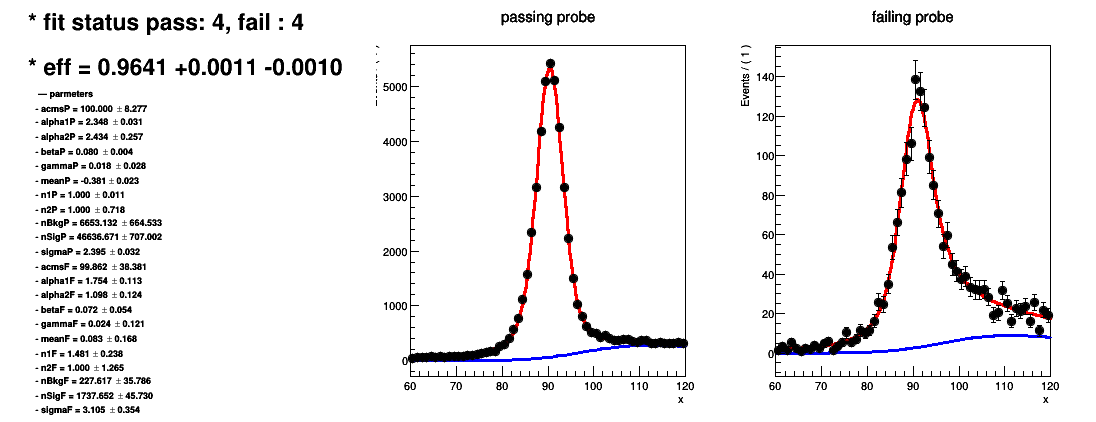
\includegraphics[height=0.355\textheight]{fits/wNF/seed_EB_R9_0p55to0p85_et70.png}\\[2pt]
  \vspace{-10pt}\hfill\hyperlink{eff-seed-EB}{\beamerreturnbutton{efficiency}}
\end{frame}

\begin{frame}[label=fit-seed-EB-R9-0p55to0p85-90]{Fits: seeded leg, EB $0.55<\RNine<0.85$, $\ET>90$~GeV}
  \centering
  {\scriptsize\hl{without NF}}\\[1pt]
  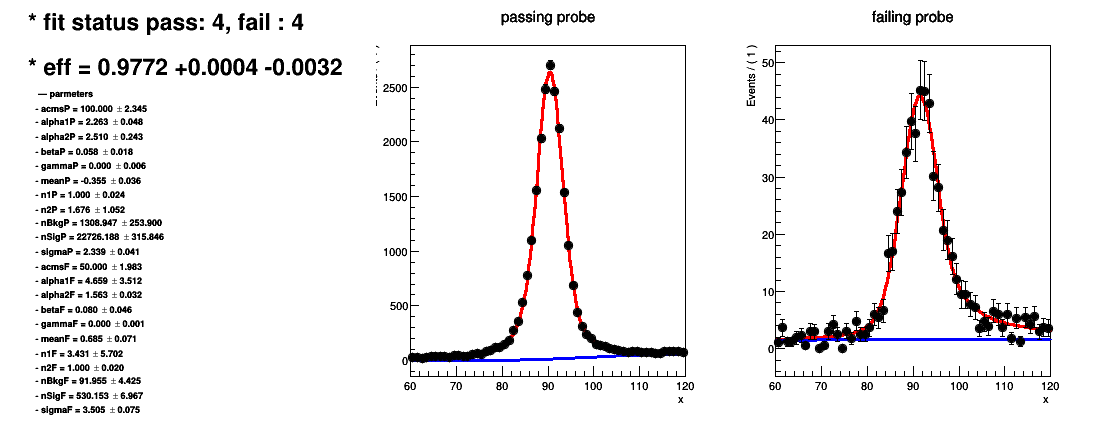
\includegraphics[height=0.355\textheight]{fits/woNF/seed_EB_R9_0p55to0p85_et90.png}\\[2pt]
  {\scriptsize\hl{with NF}}\\[1pt]
  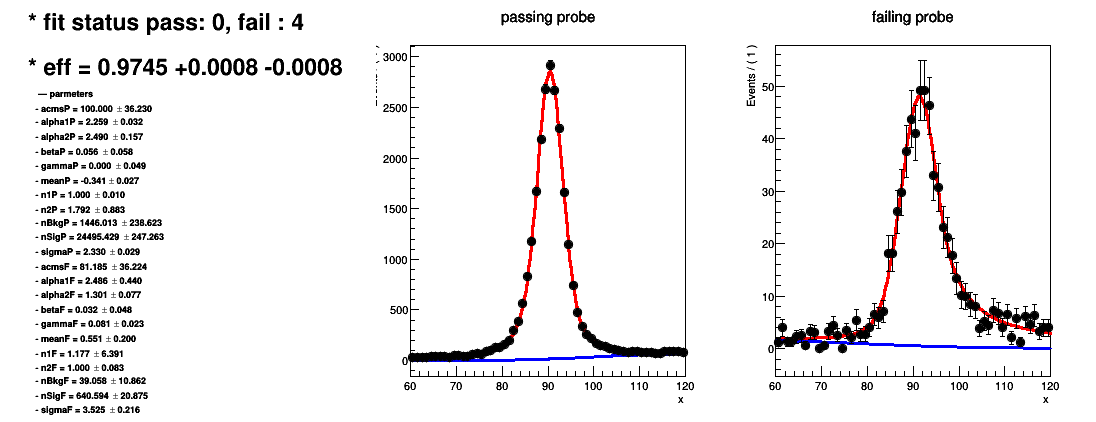
\includegraphics[height=0.355\textheight]{fits/wNF/seed_EB_R9_0p55to0p85_et90.png}\\[2pt]
  \vspace{-10pt}\hfill\hyperlink{eff-seed-EB}{\beamerreturnbutton{efficiency}}
\end{frame}

\begin{frame}[label=fit-seed-EB-R9gt0p85-0]{Fits: seeded leg, EB $\RNine>0.85$, $0<\ET<35$~GeV}
  \centering
  {\scriptsize\hl{without NF}}\\[1pt]
  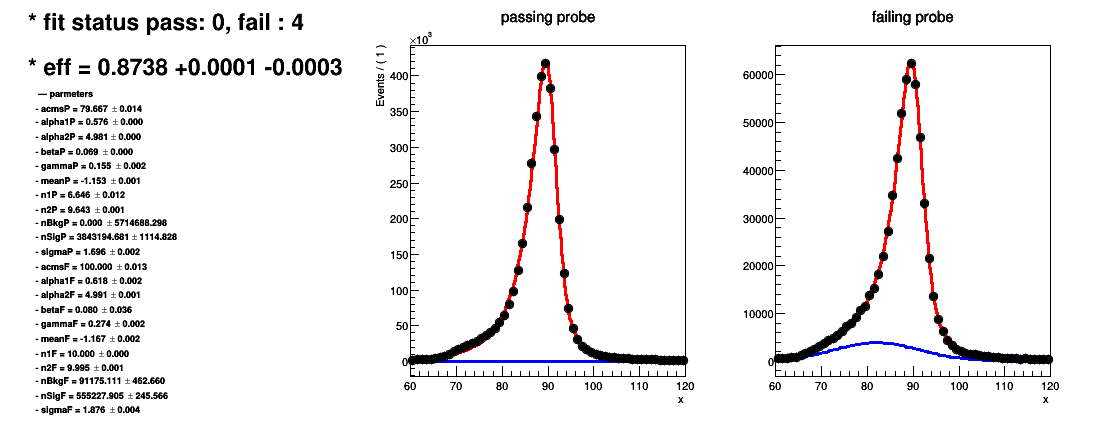
\includegraphics[height=0.355\textheight]{fits/woNF/seed_EB_R9gt0p85_et0.png}\\[2pt]
  {\scriptsize\hl{with NF}}\\[1pt]
  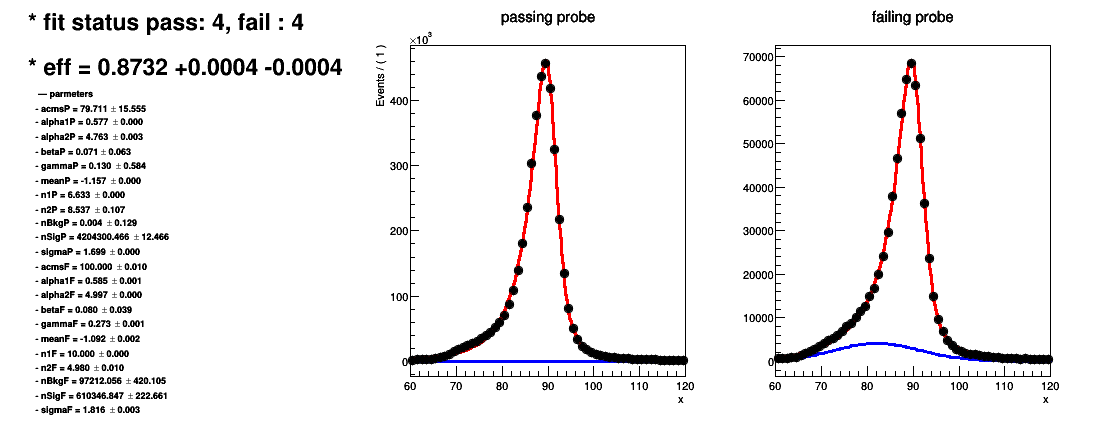
\includegraphics[height=0.355\textheight]{fits/wNF/seed_EB_R9gt0p85_et0.png}\\[2pt]
  \vspace{-10pt}\hfill\hyperlink{eff-seed-EB}{\beamerreturnbutton{efficiency}}
\end{frame}

\begin{frame}[label=fit-seed-EB-R9gt0p85-35]{Fits: seeded leg, EB $\RNine>0.85$, $35<\ET<37$~GeV}
  \centering
  {\scriptsize\hl{without NF}}\\[1pt]
  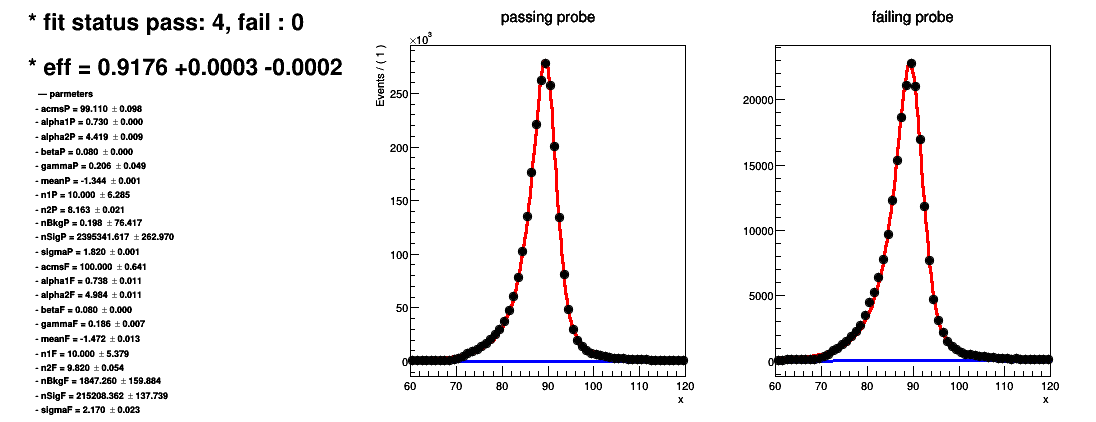
\includegraphics[height=0.355\textheight]{fits/woNF/seed_EB_R9gt0p85_et35.png}\\[2pt]
  {\scriptsize\hl{with NF}}\\[1pt]
  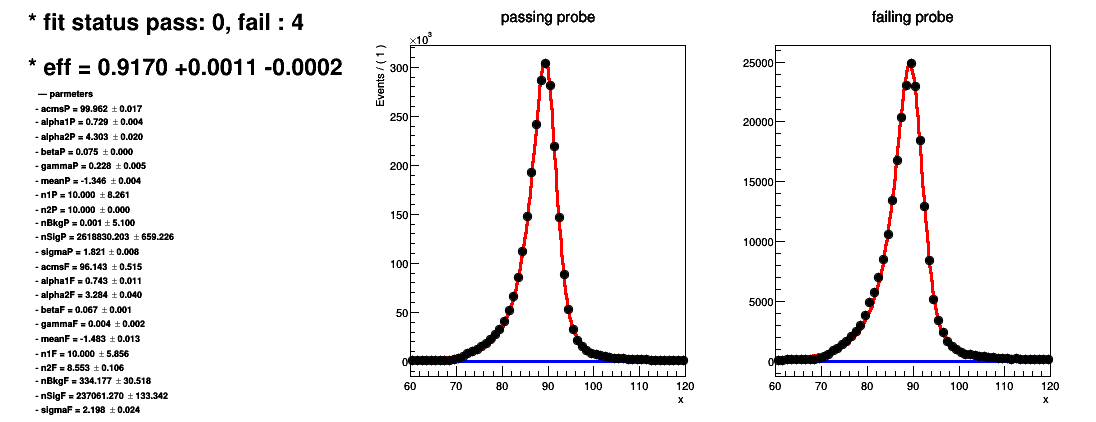
\includegraphics[height=0.355\textheight]{fits/wNF/seed_EB_R9gt0p85_et35.png}\\[2pt]
  \vspace{-10pt}\hfill\hyperlink{eff-seed-EB}{\beamerreturnbutton{efficiency}}
\end{frame}

\begin{frame}[label=fit-seed-EB-R9gt0p85-37]{Fits: seeded leg, EB $\RNine>0.85$, $37<\ET<40$~GeV}
  \centering
  {\scriptsize\hl{without NF}}\\[1pt]
  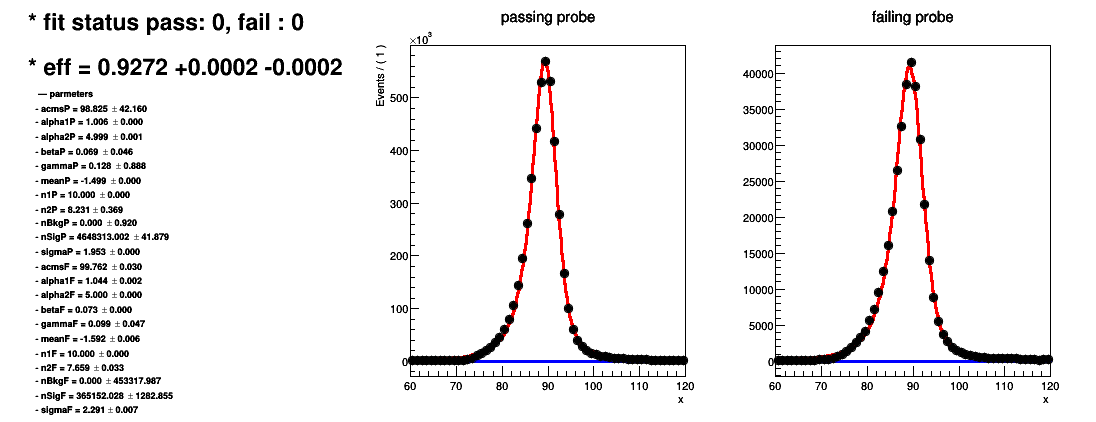
\includegraphics[height=0.355\textheight]{fits/woNF/seed_EB_R9gt0p85_et37.png}\\[2pt]
  {\scriptsize\hl{with NF}}\\[1pt]
  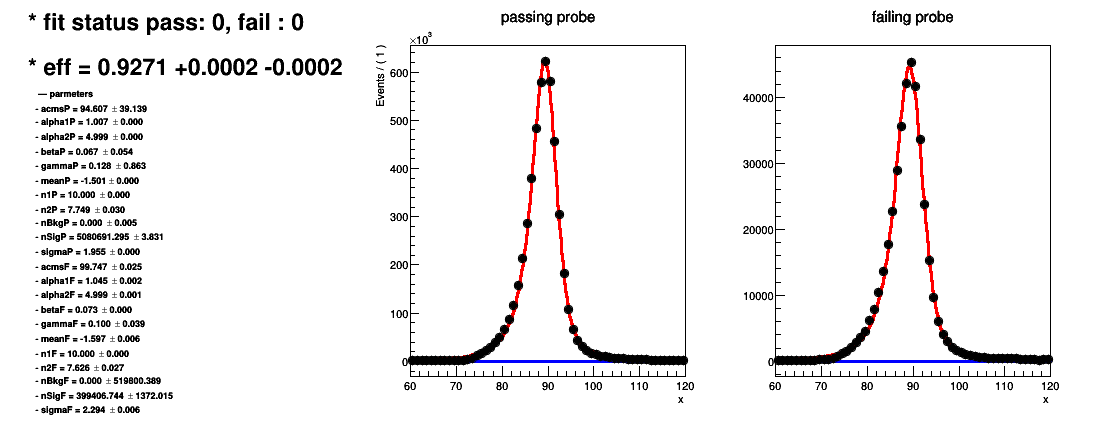
\includegraphics[height=0.355\textheight]{fits/wNF/seed_EB_R9gt0p85_et37.png}\\[2pt]
  \vspace{-10pt}\hfill\hyperlink{eff-seed-EB}{\beamerreturnbutton{efficiency}}
\end{frame}

\begin{frame}[label=fit-seed-EB-R9gt0p85-40]{Fits: seeded leg, EB $\RNine>0.85$, $40<\ET<45$~GeV}
  \centering
  {\scriptsize\hl{without NF}}\\[1pt]
  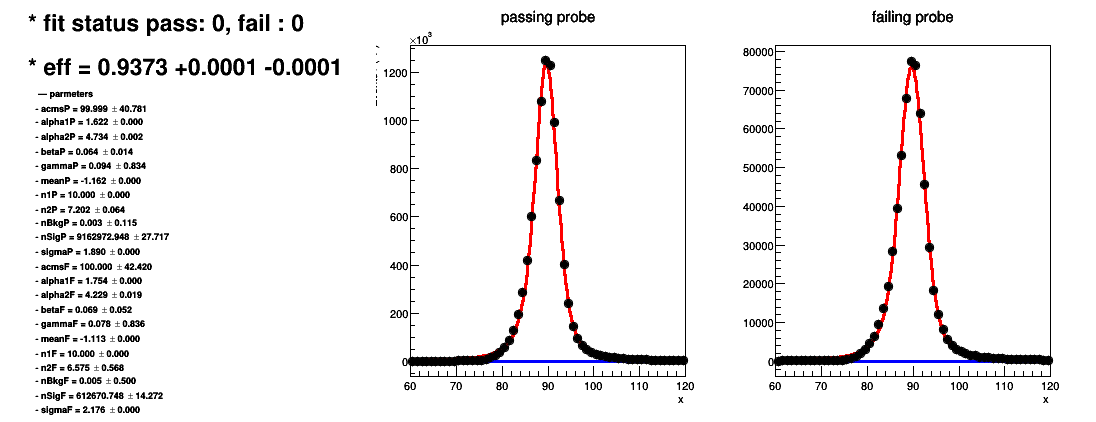
\includegraphics[height=0.355\textheight]{fits/woNF/seed_EB_R9gt0p85_et40.png}\\[2pt]
  {\scriptsize\hl{with NF}}\\[1pt]
  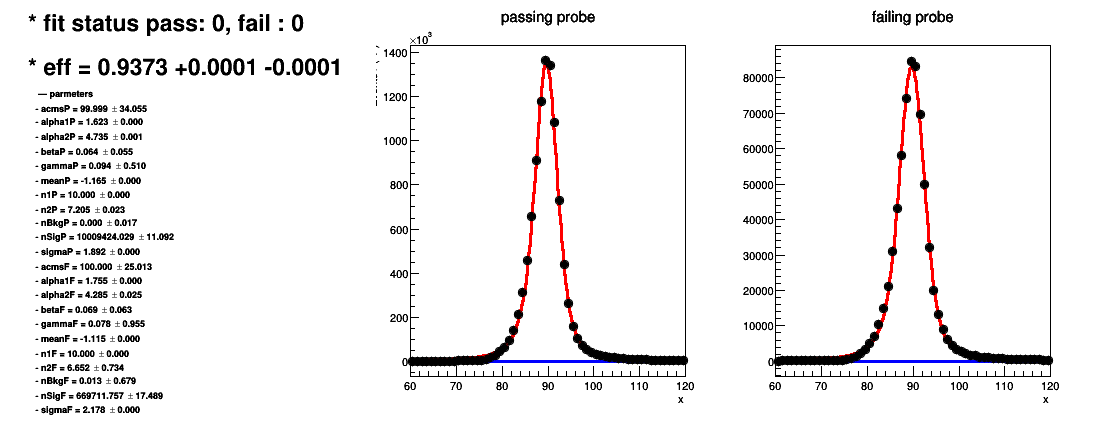
\includegraphics[height=0.355\textheight]{fits/wNF/seed_EB_R9gt0p85_et40.png}\\[2pt]
  \vspace{-10pt}\hfill\hyperlink{eff-seed-EB}{\beamerreturnbutton{efficiency}}
\end{frame}

\begin{frame}[label=fit-seed-EB-R9gt0p85-45]{Fits: seeded leg, EB $\RNine>0.85$, $45<\ET<50$~GeV}
  \centering
  {\scriptsize\hl{without NF}}\\[1pt]
  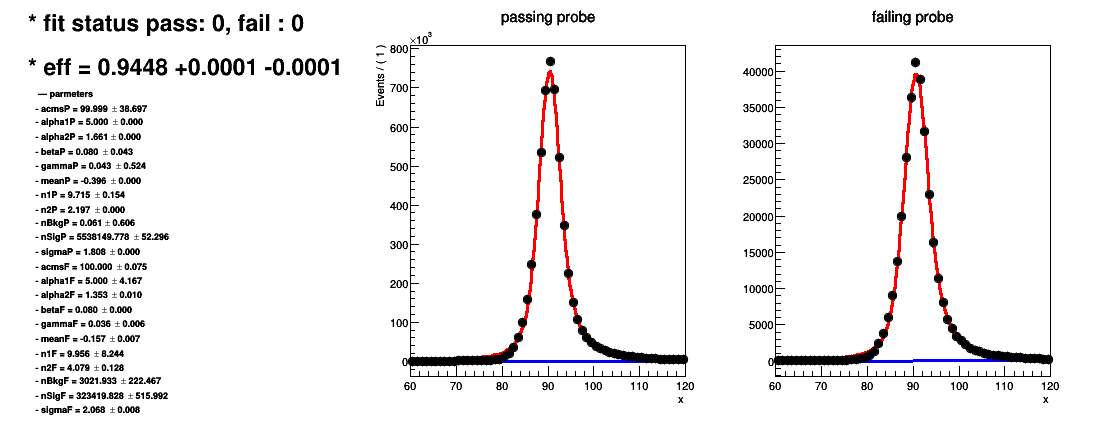
\includegraphics[height=0.355\textheight]{fits/woNF/seed_EB_R9gt0p85_et45.png}\\[2pt]
  {\scriptsize\hl{with NF}}\\[1pt]
  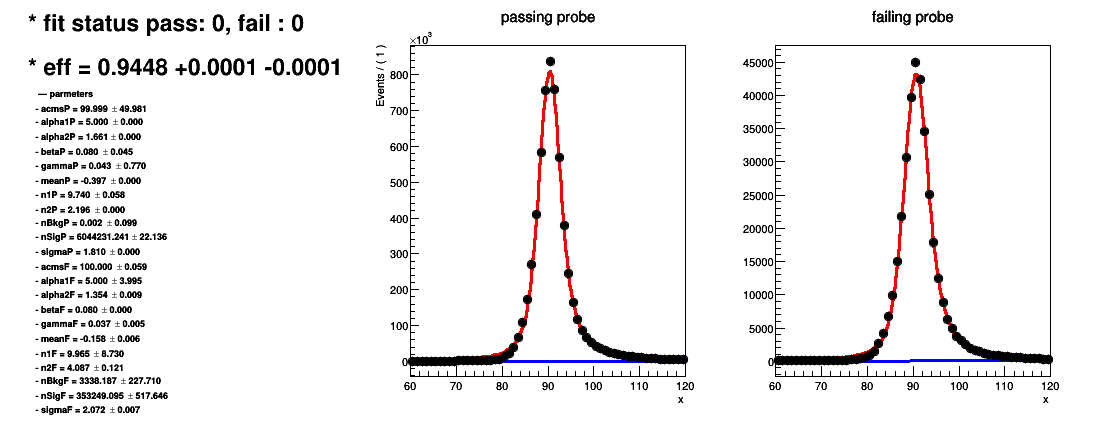
\includegraphics[height=0.355\textheight]{fits/wNF/seed_EB_R9gt0p85_et45.png}\\[2pt]
  \vspace{-10pt}\hfill\hyperlink{eff-seed-EB}{\beamerreturnbutton{efficiency}}
\end{frame}

\begin{frame}[label=fit-seed-EB-R9gt0p85-50]{Fits: seeded leg, EB $\RNine>0.85$, $50<\ET<60$~GeV}
  \centering
  {\scriptsize\hl{without NF}}\\[1pt]
  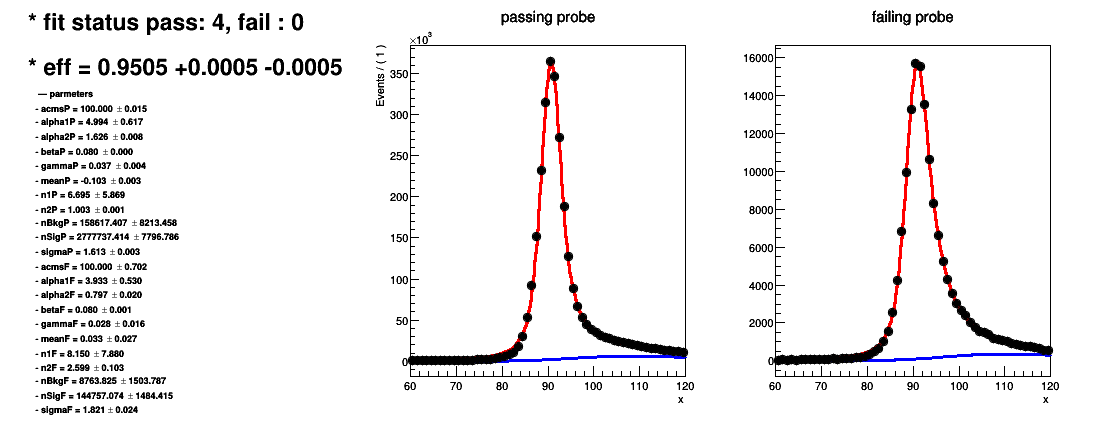
\includegraphics[height=0.355\textheight]{fits/woNF/seed_EB_R9gt0p85_et50.png}\\[2pt]
  {\scriptsize\hl{with NF}}\\[1pt]
  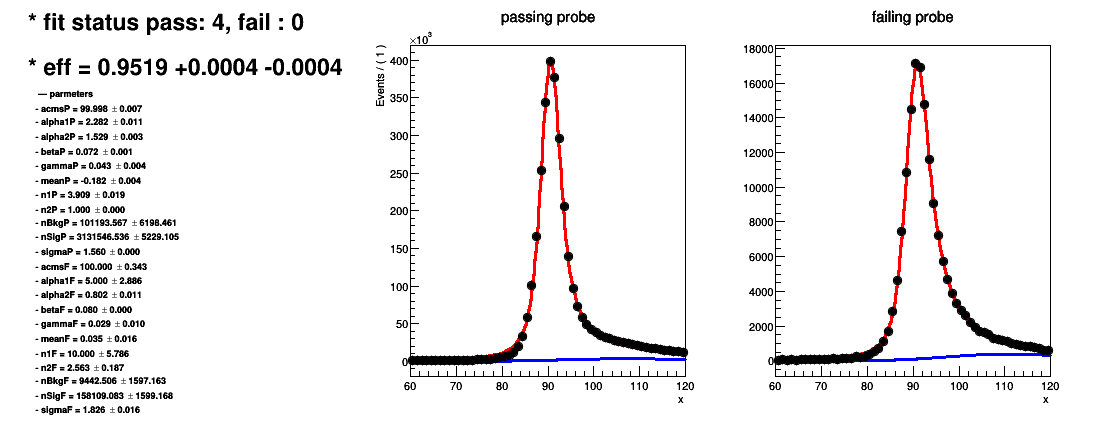
\includegraphics[height=0.355\textheight]{fits/wNF/seed_EB_R9gt0p85_et50.png}\\[2pt]
  \vspace{-10pt}\hfill\hyperlink{eff-seed-EB}{\beamerreturnbutton{efficiency}}
\end{frame}

\begin{frame}[label=fit-seed-EB-R9gt0p85-60]{Fits: seeded leg, EB $\RNine>0.85$, $60<\ET<70$~GeV}
  \centering
  {\scriptsize\hl{without NF}}\\[1pt]
  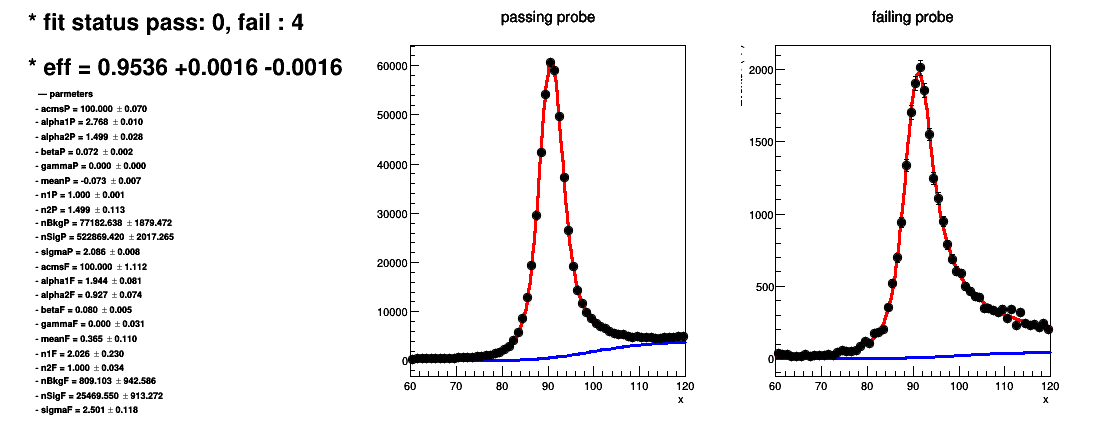
\includegraphics[height=0.355\textheight]{fits/woNF/seed_EB_R9gt0p85_et60.png}\\[2pt]
  {\scriptsize\hl{with NF}}\\[1pt]
  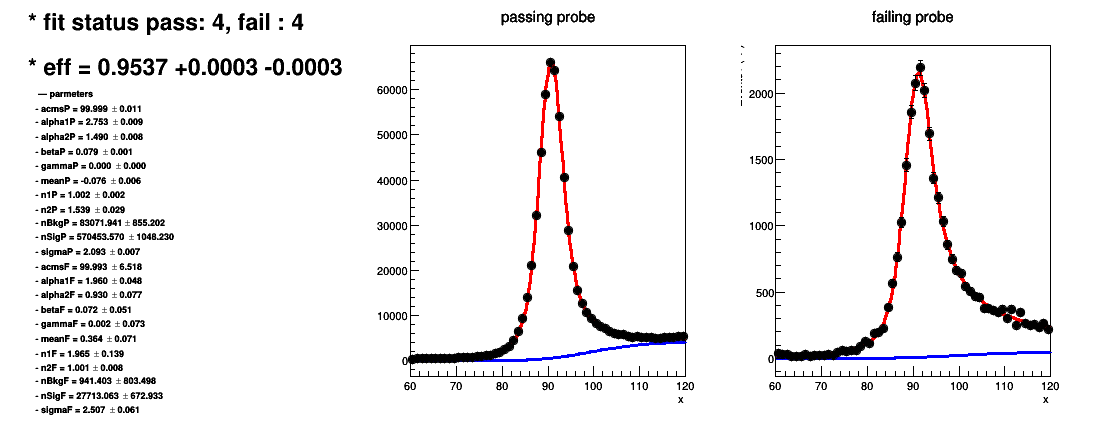
\includegraphics[height=0.355\textheight]{fits/wNF/seed_EB_R9gt0p85_et60.png}\\[2pt]
  \vspace{-10pt}\hfill\hyperlink{eff-seed-EB}{\beamerreturnbutton{efficiency}}
\end{frame}

\begin{frame}[label=fit-seed-EB-R9gt0p85-70]{Fits: seeded leg, EB $\RNine>0.85$, $70<\ET<90$~GeV}
  \centering
  {\scriptsize\hl{without NF}}\\[1pt]
  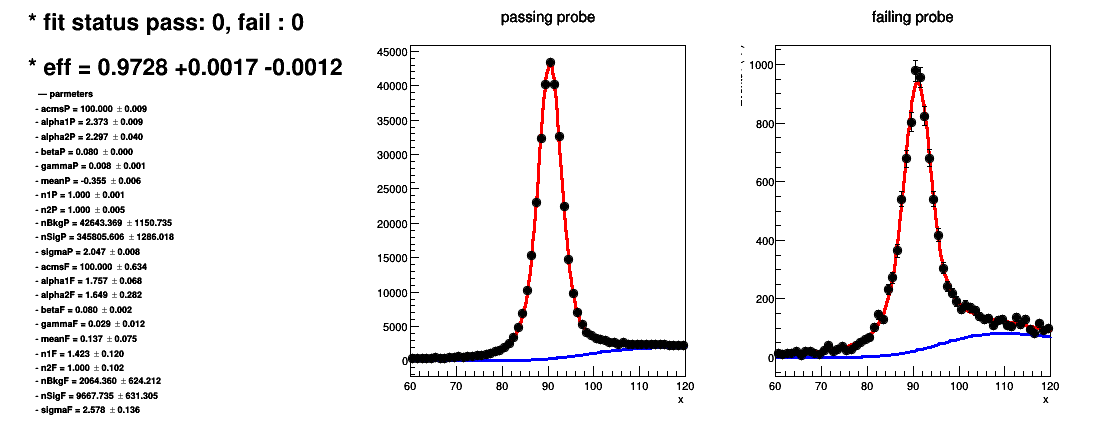
\includegraphics[height=0.355\textheight]{fits/woNF/seed_EB_R9gt0p85_et70.png}\\[2pt]
  {\scriptsize\hl{with NF}}\\[1pt]
  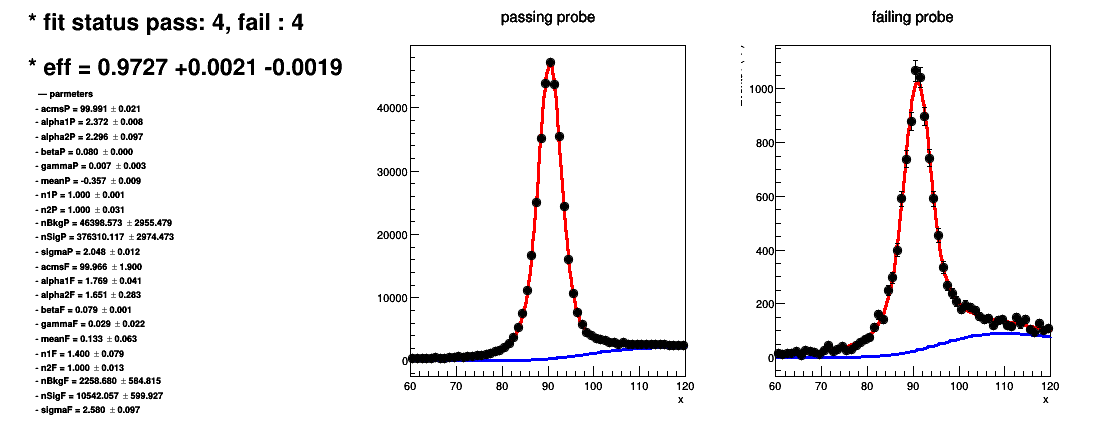
\includegraphics[height=0.355\textheight]{fits/wNF/seed_EB_R9gt0p85_et70.png}\\[2pt]
  \vspace{-10pt}\hfill\hyperlink{eff-seed-EB}{\beamerreturnbutton{efficiency}}
\end{frame}

\begin{frame}[label=fit-seed-EB-R9gt0p85-90]{Fits: seeded leg, EB $\RNine>0.85$, $\ET>90$~GeV}
  \centering
  {\scriptsize\hl{without NF}}\\[1pt]
  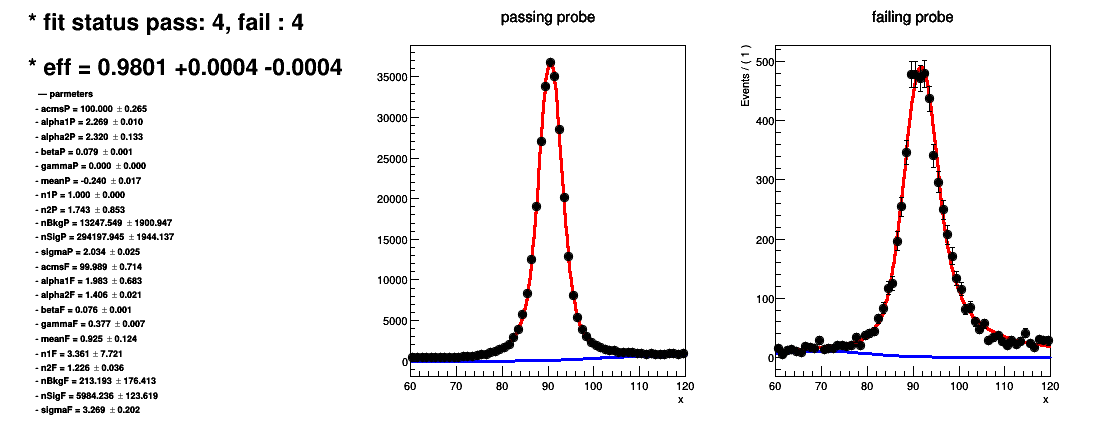
\includegraphics[height=0.355\textheight]{fits/woNF/seed_EB_R9gt0p85_et90.png}\\[2pt]
  {\scriptsize\hl{with NF}}\\[1pt]
  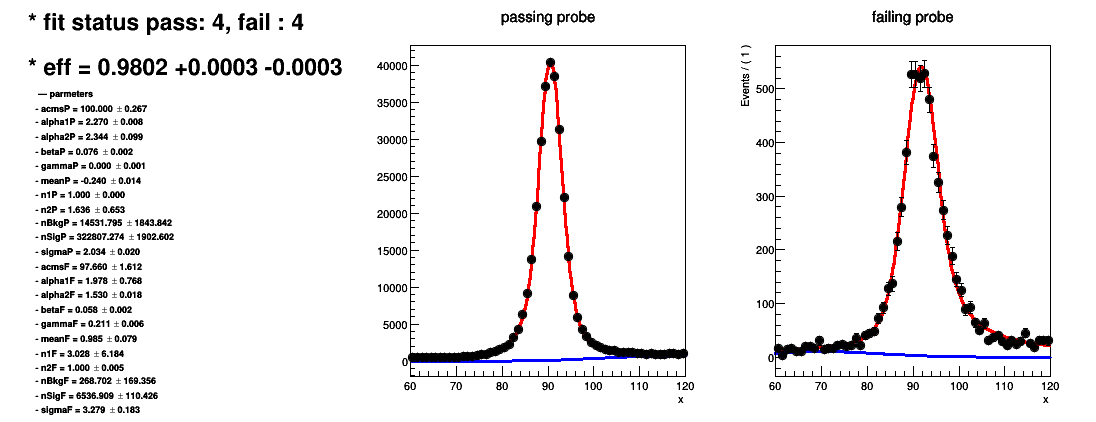
\includegraphics[height=0.355\textheight]{fits/wNF/seed_EB_R9gt0p85_et90.png}\\[2pt]
  \vspace{-10pt}\hfill\hyperlink{eff-seed-EB}{\beamerreturnbutton{efficiency}}
\end{frame}

\begin{frame}[label=fit-seed-EE-R9-0p90to0p93-0]{Fits: seeded leg, EE $0.90<\RNine<0.93$, $0<\ET<35$~GeV}
  \centering
  {\scriptsize\hl{without NF}}\\[1pt]
  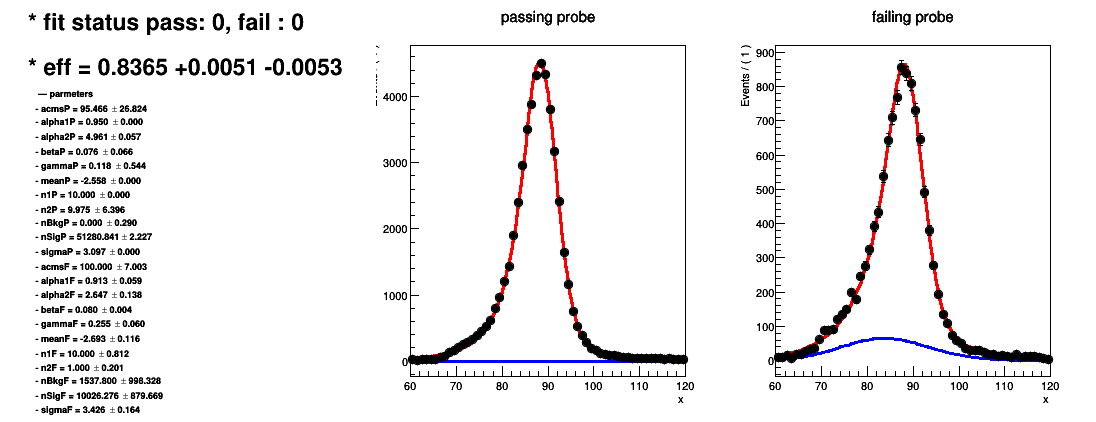
\includegraphics[height=0.355\textheight]{fits/woNF/seed_EE_R9_0p90to0p93_et0.png}\\[2pt]
  {\scriptsize\hl{with NF}}\\[1pt]
  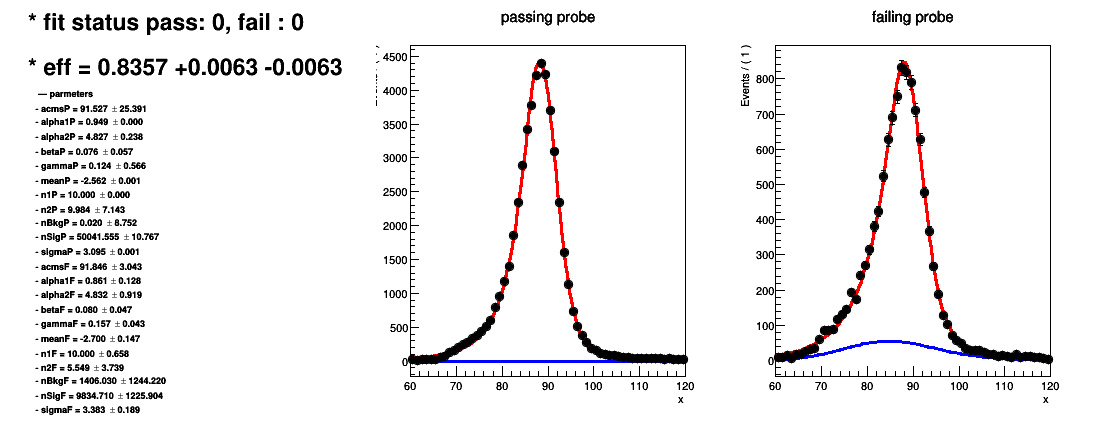
\includegraphics[height=0.355\textheight]{fits/wNF/seed_EE_R9_0p90to0p93_et0.png}\\[2pt]
  \vspace{-10pt}\hfill\hyperlink{eff-seed-EE}{\beamerreturnbutton{efficiency}}
\end{frame}

\begin{frame}[label=fit-seed-EE-R9-0p90to0p93-35]{Fits: seeded leg, EE $0.90<\RNine<0.93$, $35<\ET<37$~GeV}
  \centering
  {\scriptsize\hl{without NF}}\\[1pt]
  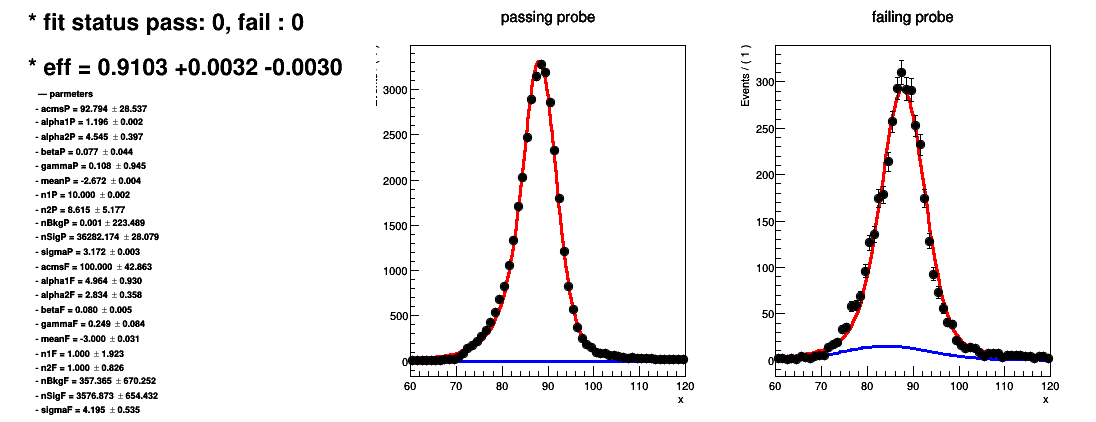
\includegraphics[height=0.355\textheight]{fits/woNF/seed_EE_R9_0p90to0p93_et35.png}\\[2pt]
  {\scriptsize\hl{with NF}}\\[1pt]
  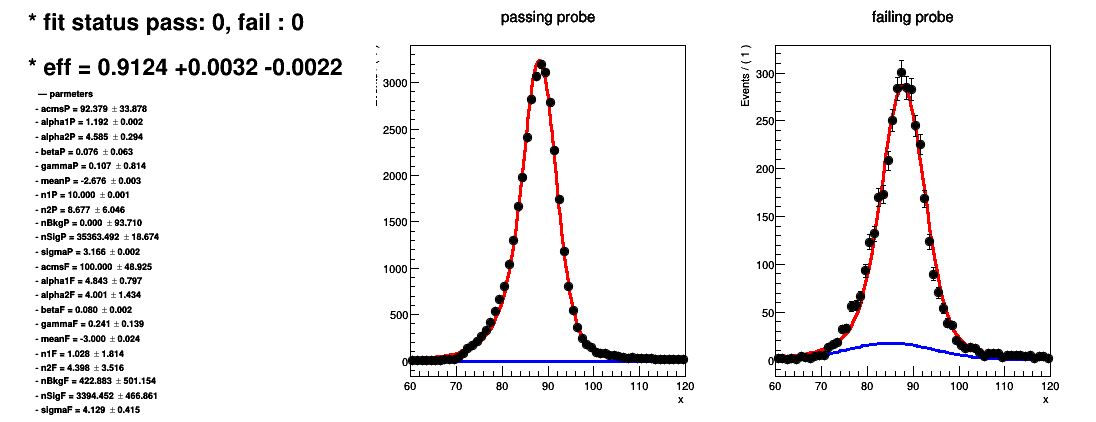
\includegraphics[height=0.355\textheight]{fits/wNF/seed_EE_R9_0p90to0p93_et35.png}\\[2pt]
  \vspace{-10pt}\hfill\hyperlink{eff-seed-EE}{\beamerreturnbutton{efficiency}}
\end{frame}

\begin{frame}[label=fit-seed-EE-R9-0p90to0p93-37]{Fits: seeded leg, EE $0.90<\RNine<0.93$, $37<\ET<40$~GeV}
  \centering
  {\scriptsize\hl{without NF}}\\[1pt]
  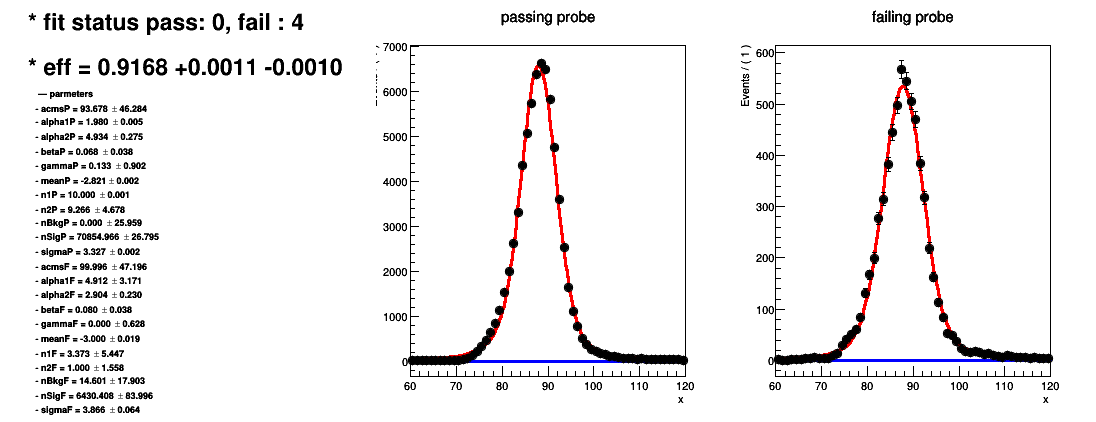
\includegraphics[height=0.355\textheight]{fits/woNF/seed_EE_R9_0p90to0p93_et37.png}\\[2pt]
  {\scriptsize\hl{with NF}}\\[1pt]
  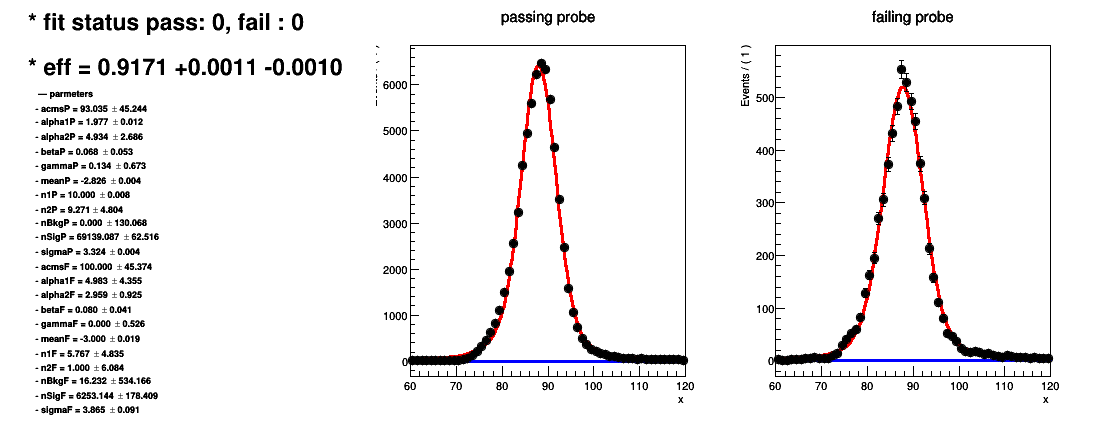
\includegraphics[height=0.355\textheight]{fits/wNF/seed_EE_R9_0p90to0p93_et37.png}\\[2pt]
  \vspace{-10pt}\hfill\hyperlink{eff-seed-EE}{\beamerreturnbutton{efficiency}}
\end{frame}

\begin{frame}[label=fit-seed-EE-R9-0p90to0p93-40]{Fits: seeded leg, EE $0.90<\RNine<0.93$, $40<\ET<45$~GeV}
  \centering
  {\scriptsize\hl{without NF}}\\[1pt]
  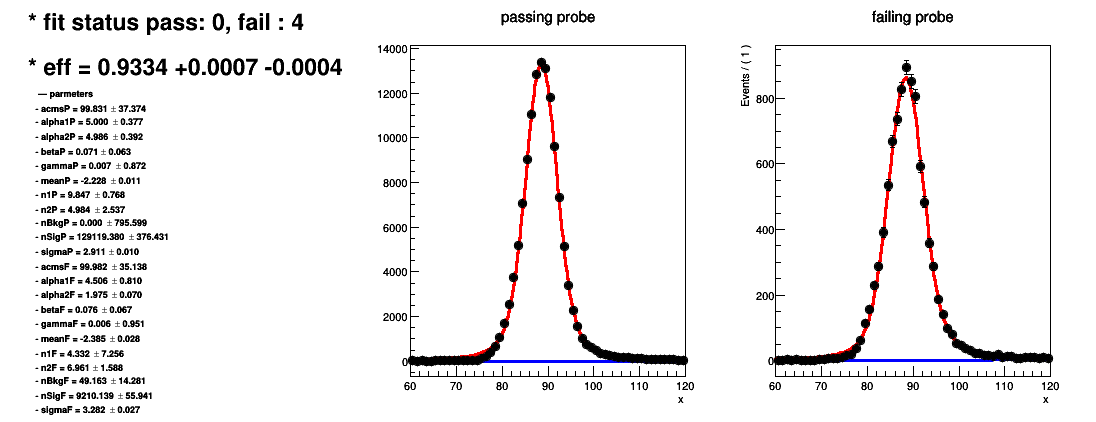
\includegraphics[height=0.355\textheight]{fits/woNF/seed_EE_R9_0p90to0p93_et40.png}\\[2pt]
  {\scriptsize\hl{with NF}}\\[1pt]
  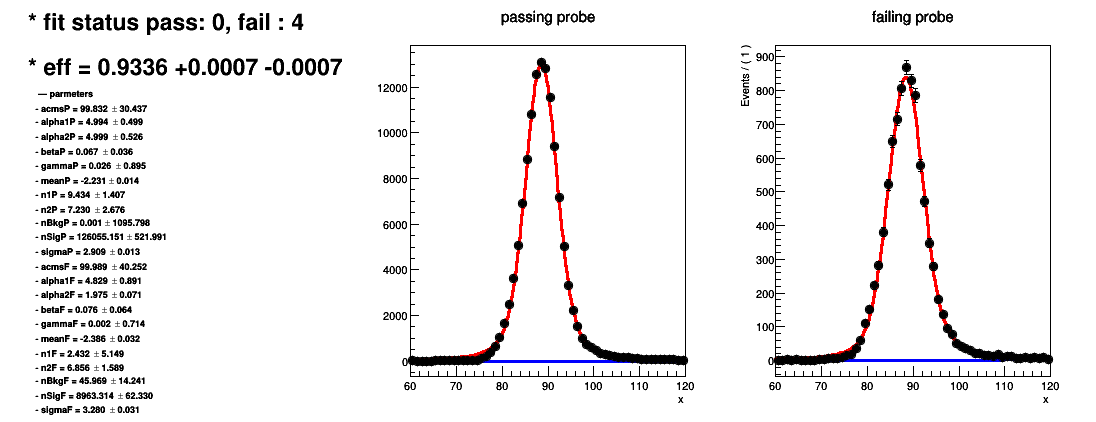
\includegraphics[height=0.355\textheight]{fits/wNF/seed_EE_R9_0p90to0p93_et40.png}\\[2pt]
  \vspace{-10pt}\hfill\hyperlink{eff-seed-EE}{\beamerreturnbutton{efficiency}}
\end{frame}

\begin{frame}[label=fit-seed-EE-R9-0p90to0p93-45]{Fits: seeded leg, EE $0.90<\RNine<0.93$, $45<\ET<50$~GeV}
  \centering
  {\scriptsize\hl{without NF}}\\[1pt]
  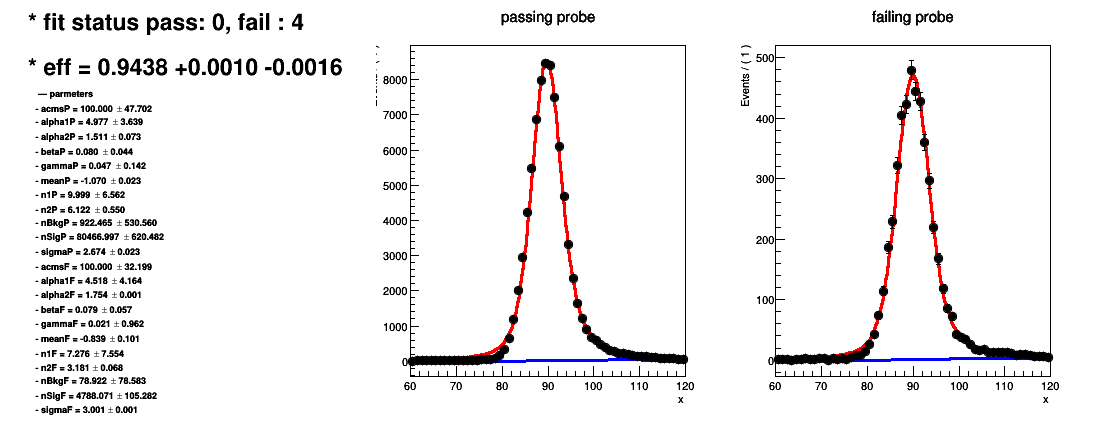
\includegraphics[height=0.355\textheight]{fits/woNF/seed_EE_R9_0p90to0p93_et45.png}\\[2pt]
  {\scriptsize\hl{with NF}}\\[1pt]
  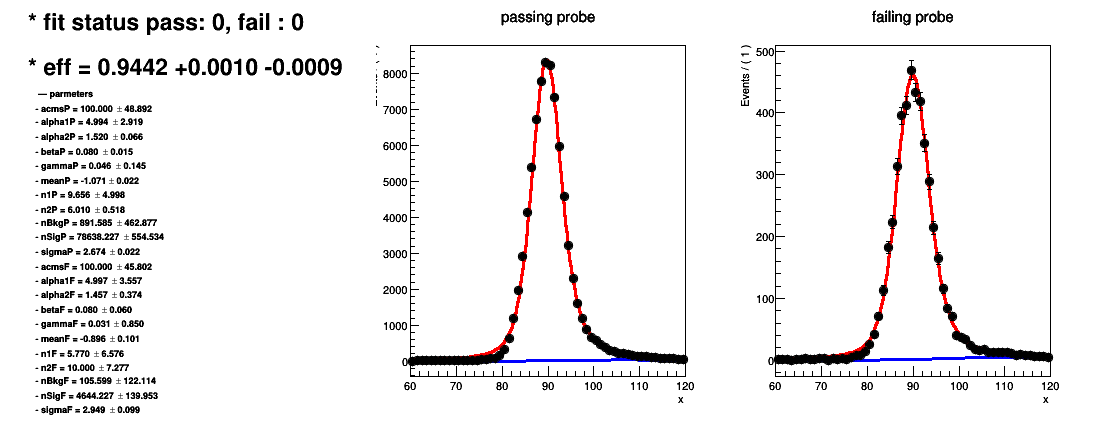
\includegraphics[height=0.355\textheight]{fits/wNF/seed_EE_R9_0p90to0p93_et45.png}\\[2pt]
  \vspace{-10pt}\hfill\hyperlink{eff-seed-EE}{\beamerreturnbutton{efficiency}}
\end{frame}

\begin{frame}[label=fit-seed-EE-R9-0p90to0p93-50]{Fits: seeded leg, EE $0.90<\RNine<0.93$, $50<\ET<60$~GeV}
  \centering
  {\scriptsize\hl{without NF}}\\[1pt]
  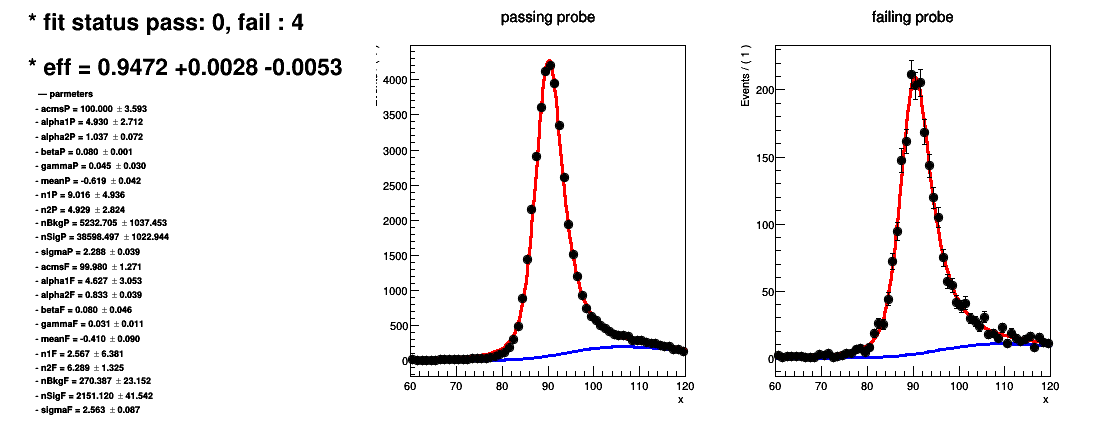
\includegraphics[height=0.355\textheight]{fits/woNF/seed_EE_R9_0p90to0p93_et50.png}\\[2pt]
  {\scriptsize\hl{with NF}}\\[1pt]
  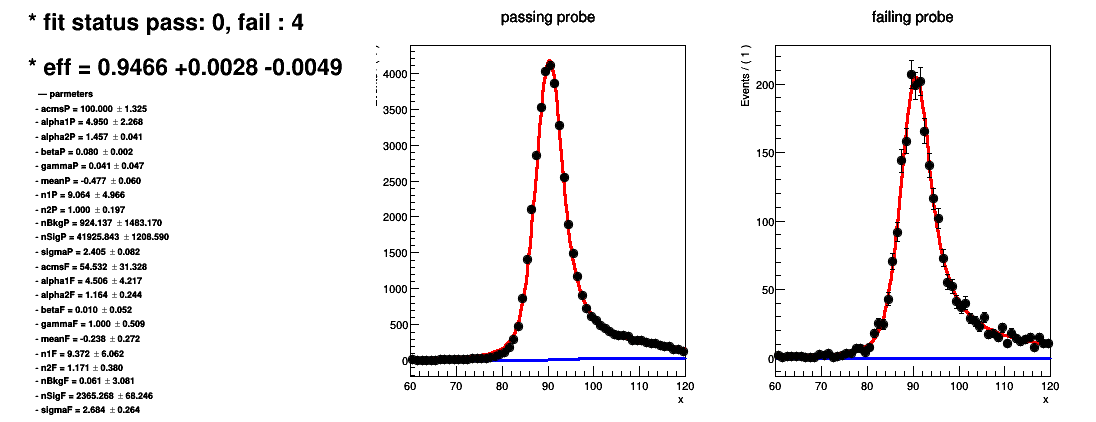
\includegraphics[height=0.355\textheight]{fits/wNF/seed_EE_R9_0p90to0p93_et50.png}\\[2pt]
  \vspace{-10pt}\hfill\hyperlink{eff-seed-EE}{\beamerreturnbutton{efficiency}}
\end{frame}

\begin{frame}[label=fit-seed-EE-R9-0p90to0p93-60]{Fits: seeded leg, EE $0.90<\RNine<0.93$, $60<\ET<70$~GeV}
  \centering
  {\scriptsize\hl{without NF}}\\[1pt]
  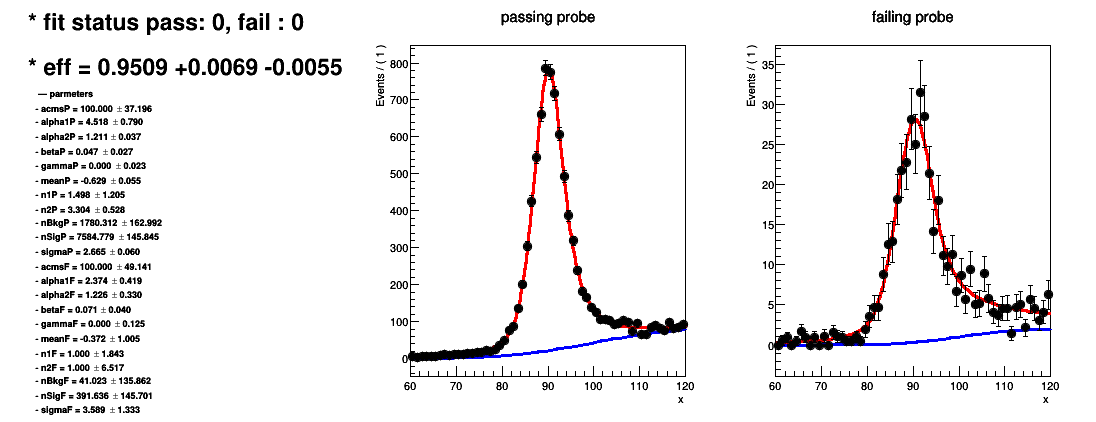
\includegraphics[height=0.355\textheight]{fits/woNF/seed_EE_R9_0p90to0p93_et60.png}\\[2pt]
  {\scriptsize\hl{with NF}}\\[1pt]
  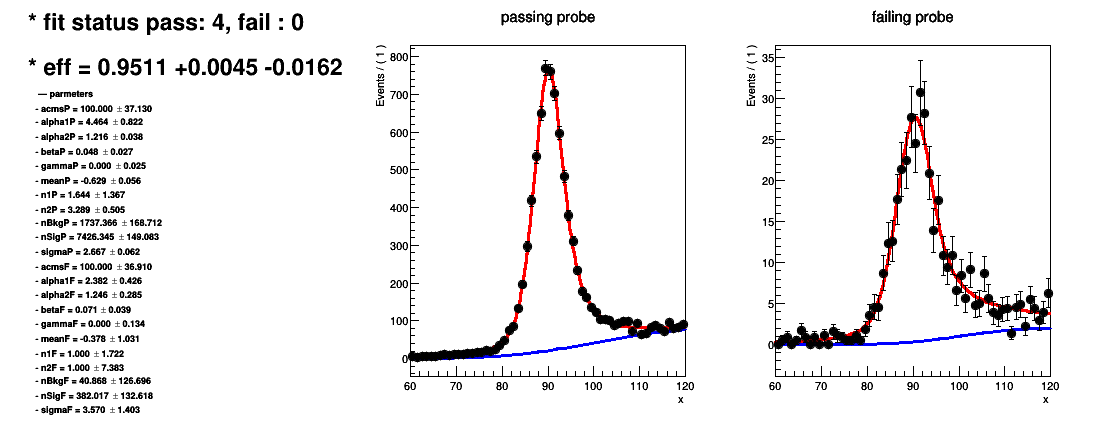
\includegraphics[height=0.355\textheight]{fits/wNF/seed_EE_R9_0p90to0p93_et60.png}\\[2pt]
  \vspace{-10pt}\hfill\hyperlink{eff-seed-EE}{\beamerreturnbutton{efficiency}}
\end{frame}

\begin{frame}[label=fit-seed-EE-R9-0p90to0p93-70]{Fits: seeded leg, EE $0.90<\RNine<0.93$, $70<\ET<90$~GeV}
  \centering
  {\scriptsize\hl{without NF}}\\[1pt]
  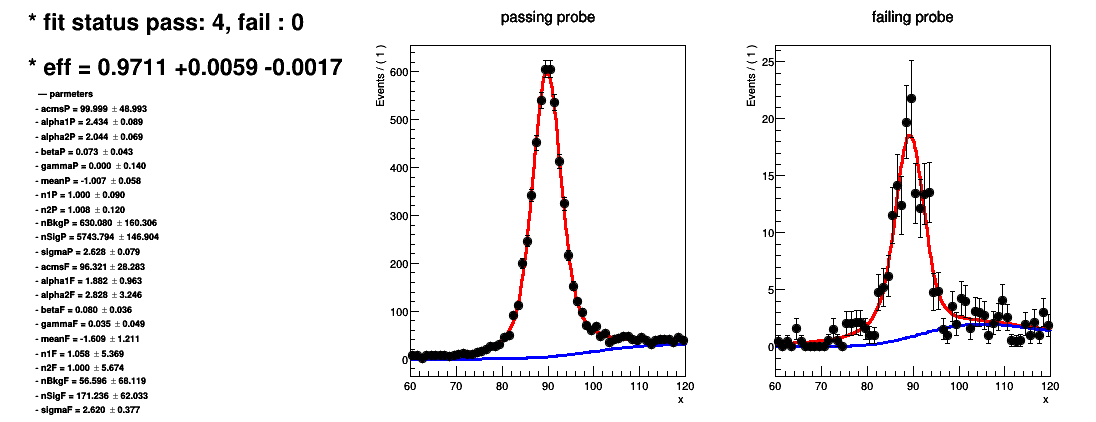
\includegraphics[height=0.355\textheight]{fits/woNF/seed_EE_R9_0p90to0p93_et70.png}\\[2pt]
  {\scriptsize\hl{with NF}}\\[1pt]
  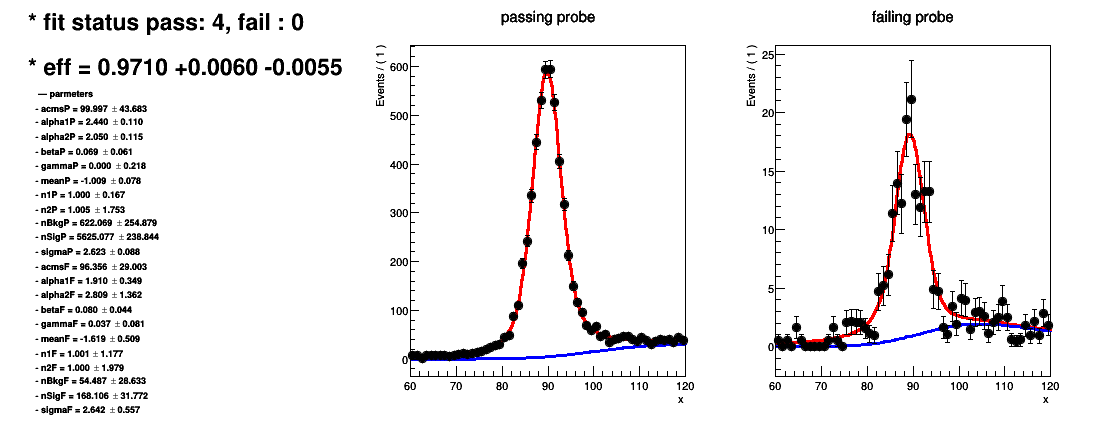
\includegraphics[height=0.355\textheight]{fits/wNF/seed_EE_R9_0p90to0p93_et70.png}\\[2pt]
  \vspace{-10pt}\hfill\hyperlink{eff-seed-EE}{\beamerreturnbutton{efficiency}}
\end{frame}

\begin{frame}[label=fit-seed-EE-R9-0p90to0p93-90]{Fits: seeded leg, EE $0.90<\RNine<0.93$, $\ET>90$~GeV}
  \centering
  {\scriptsize\hl{without NF}}\\[1pt]
  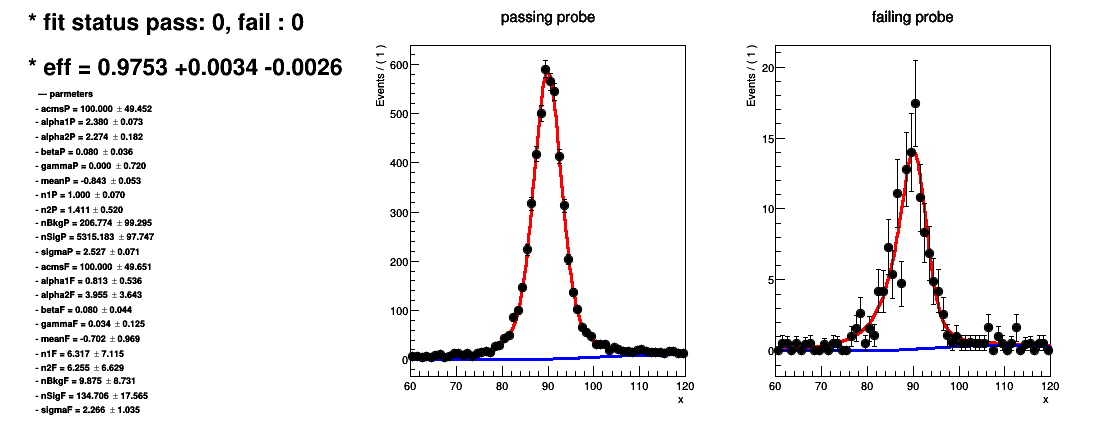
\includegraphics[height=0.355\textheight]{fits/woNF/seed_EE_R9_0p90to0p93_et90.png}\\[2pt]
  {\scriptsize\hl{with NF}}\\[1pt]
  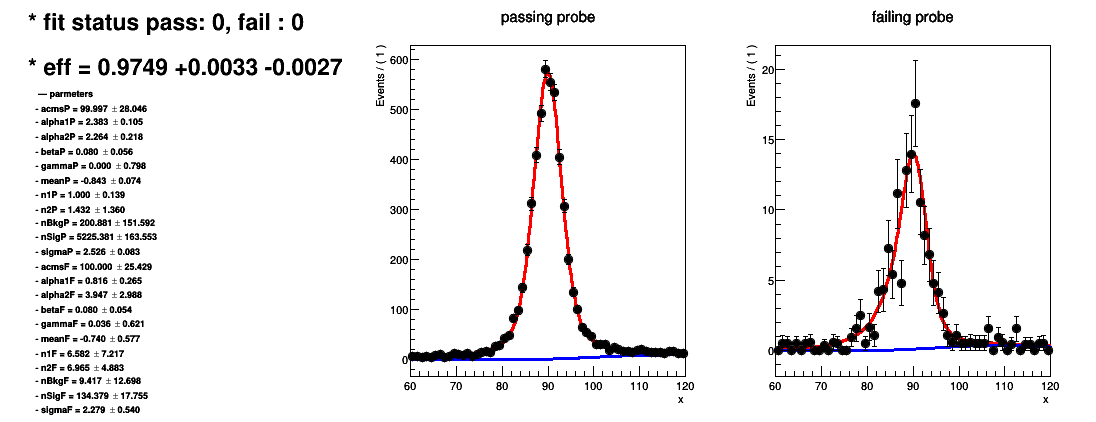
\includegraphics[height=0.355\textheight]{fits/wNF/seed_EE_R9_0p90to0p93_et90.png}\\[2pt]
  \vspace{-10pt}\hfill\hyperlink{eff-seed-EE}{\beamerreturnbutton{efficiency}}
\end{frame}

\begin{frame}[label=fit-seed-EE-R9gt0p93-0]{Fits: seeded leg, EE $\RNine>0.93$, $0<\ET<35$~GeV}
  \centering
  {\scriptsize\hl{without NF}}\\[1pt]
  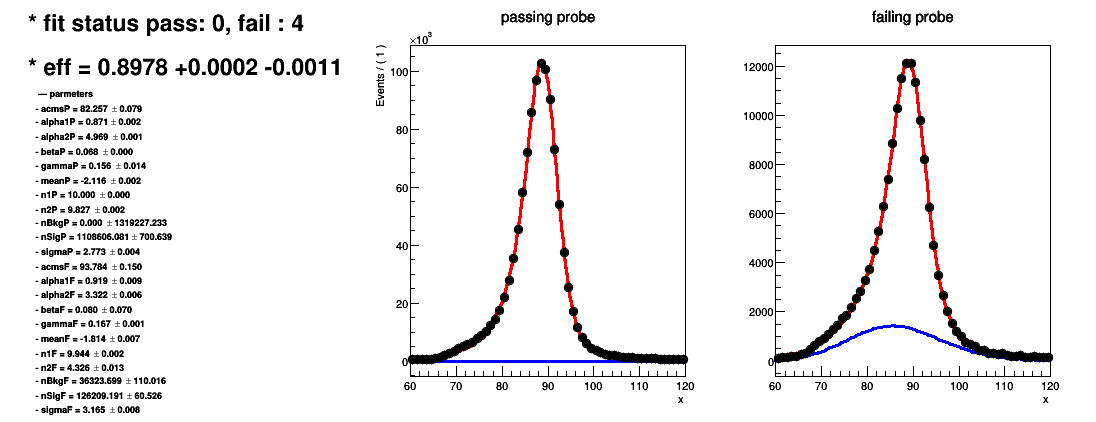
\includegraphics[height=0.355\textheight]{fits/woNF/seed_EE_R9gt0p93_et0.png}\\[2pt]
  {\scriptsize\hl{with NF}}\\[1pt]
  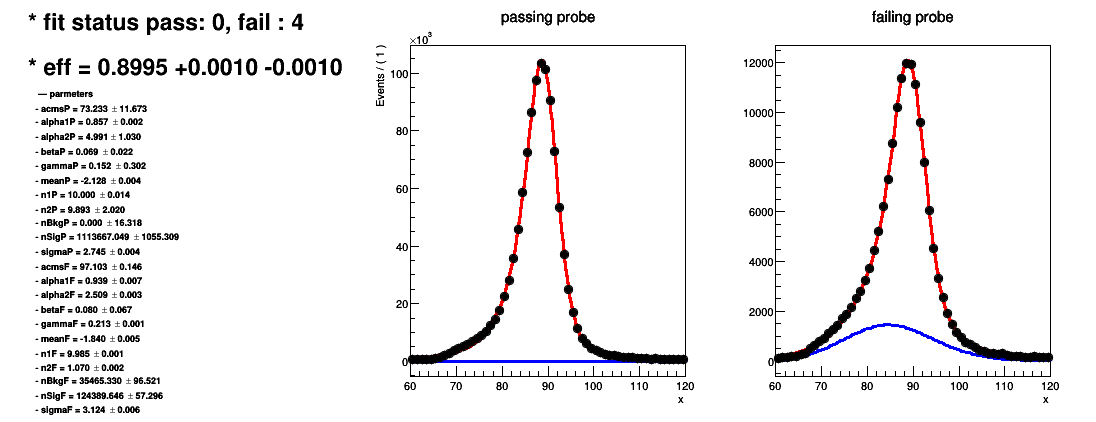
\includegraphics[height=0.355\textheight]{fits/wNF/seed_EE_R9gt0p93_et0.png}\\[2pt]
  \vspace{-10pt}\hfill\hyperlink{eff-seed-EE}{\beamerreturnbutton{efficiency}}
\end{frame}

\begin{frame}[label=fit-seed-EE-R9gt0p93-35]{Fits: seeded leg, EE $\RNine>0.93$, $35<\ET<37$~GeV}
  \centering
  {\scriptsize\hl{without NF}}\\[1pt]
  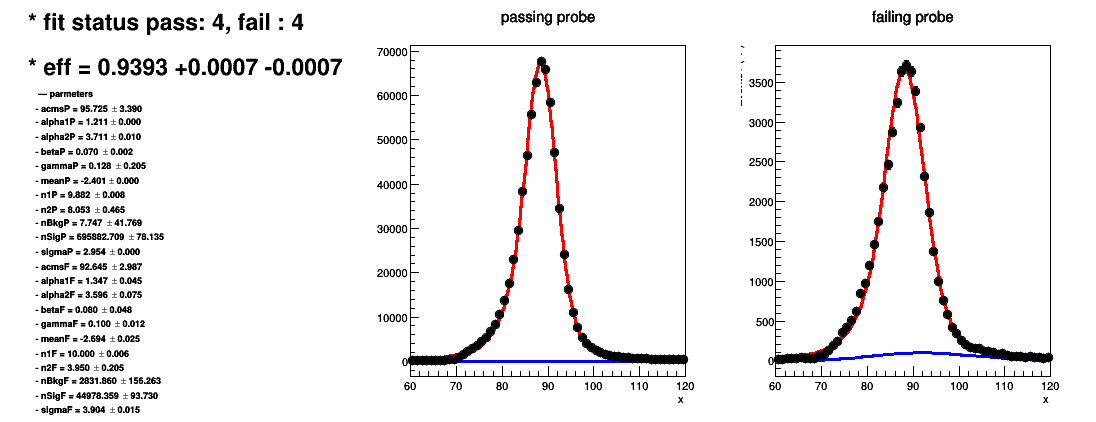
\includegraphics[height=0.355\textheight]{fits/woNF/seed_EE_R9gt0p93_et35.png}\\[2pt]
  {\scriptsize\hl{with NF}}\\[1pt]
  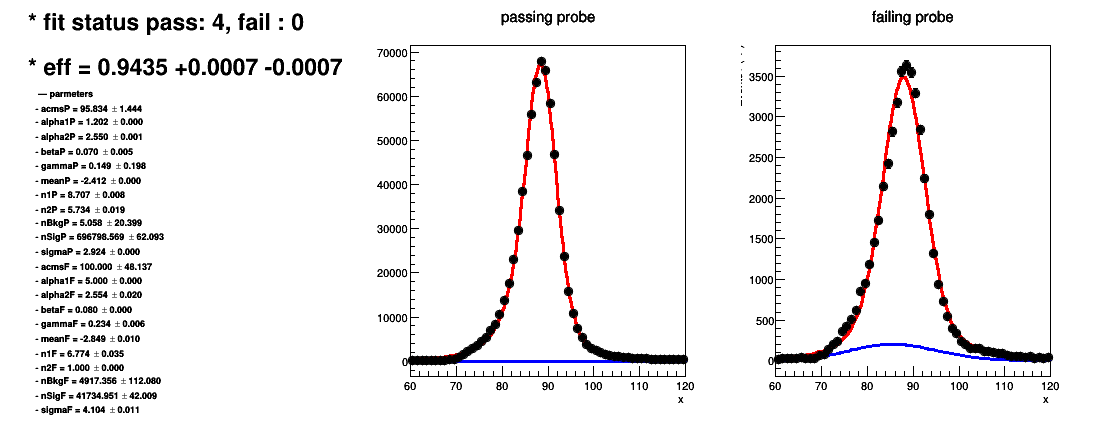
\includegraphics[height=0.355\textheight]{fits/wNF/seed_EE_R9gt0p93_et35.png}\\[2pt]
  \vspace{-10pt}\hfill\hyperlink{eff-seed-EE}{\beamerreturnbutton{efficiency}}
\end{frame}

\begin{frame}[label=fit-seed-EE-R9gt0p93-37]{Fits: seeded leg, EE $\RNine>0.93$, $37<\ET<40$~GeV}
  \centering
  {\scriptsize\hl{without NF}}\\[1pt]
  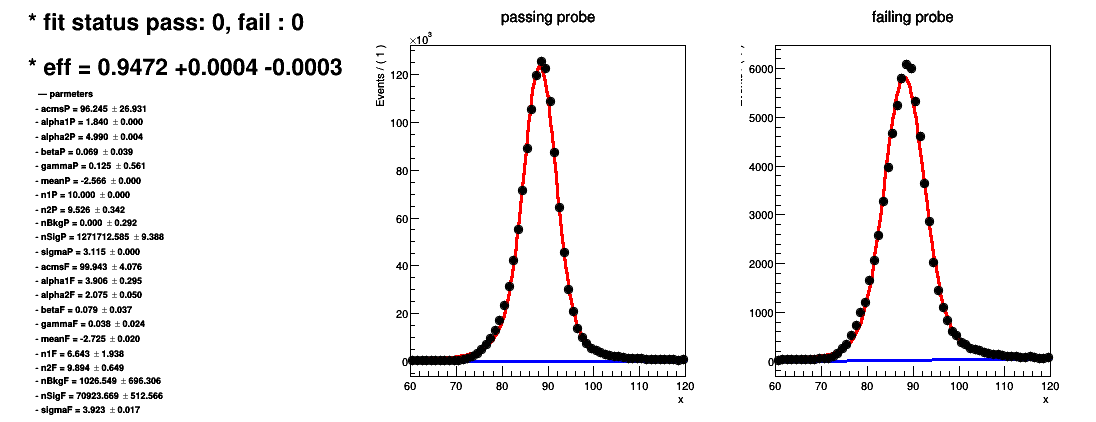
\includegraphics[height=0.355\textheight]{fits/woNF/seed_EE_R9gt0p93_et37.png}\\[2pt]
  {\scriptsize\hl{with NF}}\\[1pt]
  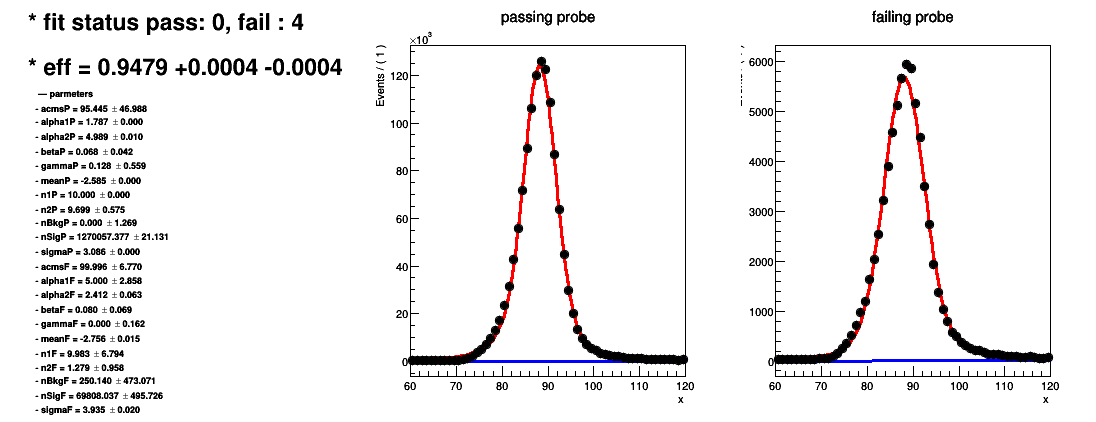
\includegraphics[height=0.355\textheight]{fits/wNF/seed_EE_R9gt0p93_et37.png}\\[2pt]
  \vspace{-10pt}\hfill\hyperlink{eff-seed-EE}{\beamerreturnbutton{efficiency}}
\end{frame}

\begin{frame}[label=fit-seed-EE-R9gt0p93-40]{Fits: seeded leg, EE $\RNine>0.93$, $40<\ET<45$~GeV}
  \centering
  {\scriptsize\hl{without NF}}\\[1pt]
  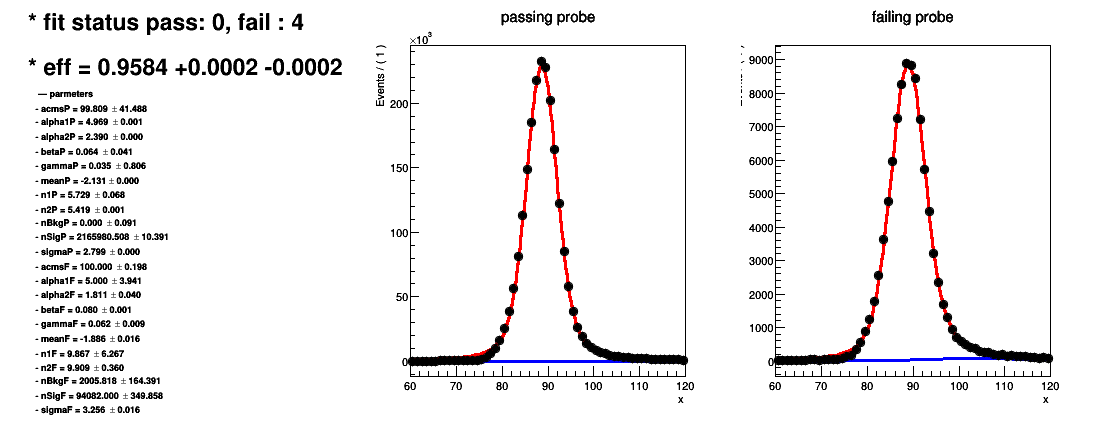
\includegraphics[height=0.355\textheight]{fits/woNF/seed_EE_R9gt0p93_et40.png}\\[2pt]
  {\scriptsize\hl{with NF}}\\[1pt]
  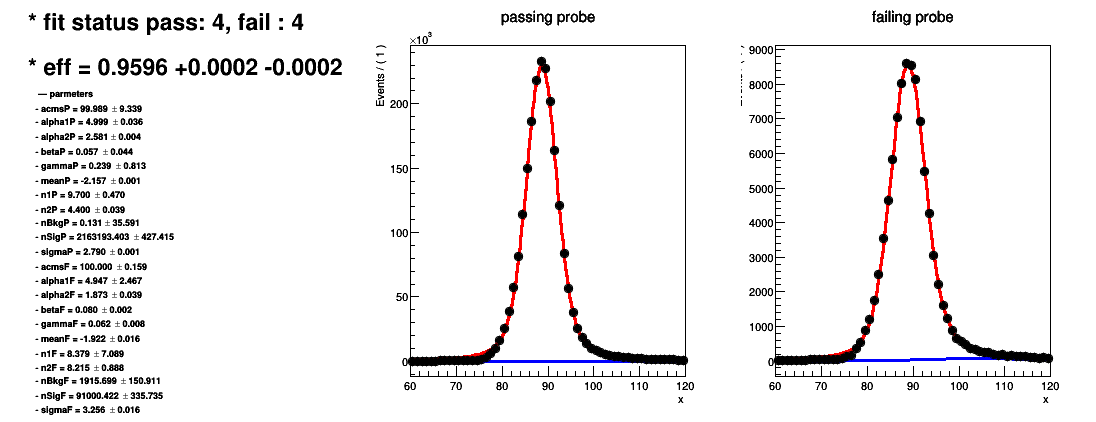
\includegraphics[height=0.355\textheight]{fits/wNF/seed_EE_R9gt0p93_et40.png}\\[2pt]
  \vspace{-10pt}\hfill\hyperlink{eff-seed-EE}{\beamerreturnbutton{efficiency}}
\end{frame}

\begin{frame}[label=fit-seed-EE-R9gt0p93-45]{Fits: seeded leg, EE $\RNine>0.93$, $45<\ET<50$~GeV}
  \centering
  {\scriptsize\hl{without NF}}\\[1pt]
  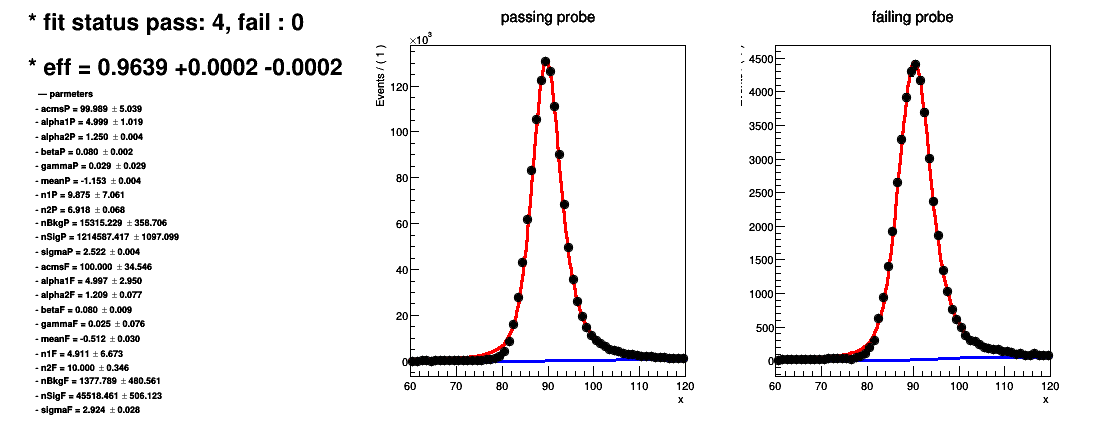
\includegraphics[height=0.355\textheight]{fits/woNF/seed_EE_R9gt0p93_et45.png}\\[2pt]
  {\scriptsize\hl{with NF}}\\[1pt]
  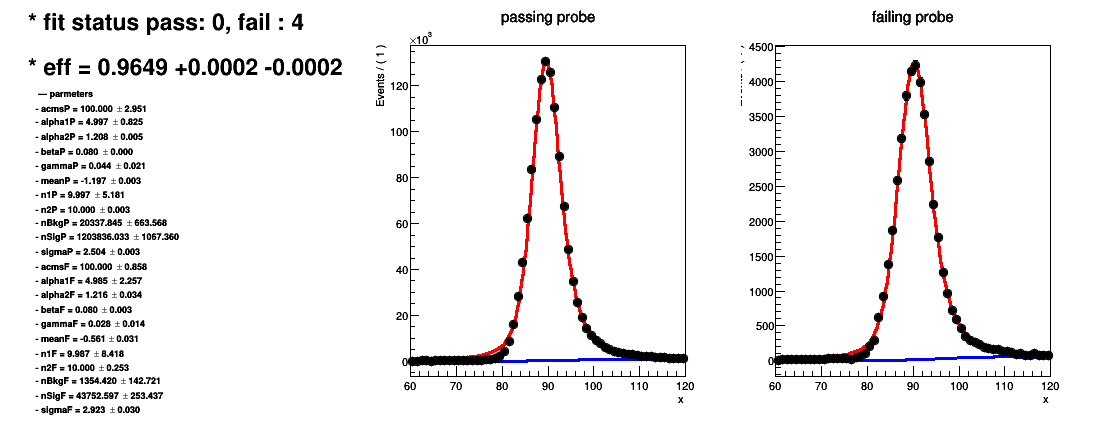
\includegraphics[height=0.355\textheight]{fits/wNF/seed_EE_R9gt0p93_et45.png}\\[2pt]
  \vspace{-10pt}\hfill\hyperlink{eff-seed-EE}{\beamerreturnbutton{efficiency}}
\end{frame}

\begin{frame}[label=fit-seed-EE-R9gt0p93-50]{Fits: seeded leg, EE $\RNine>0.93$, $50<\ET<60$~GeV}
  \centering
  {\scriptsize\hl{without NF}}\\[1pt]
  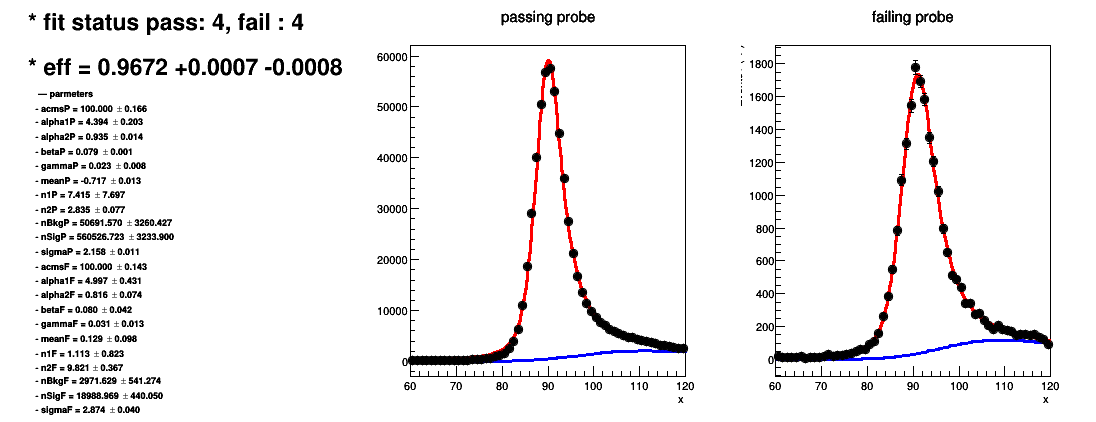
\includegraphics[height=0.355\textheight]{fits/woNF/seed_EE_R9gt0p93_et50.png}\\[2pt]
  {\scriptsize\hl{with NF}}\\[1pt]
  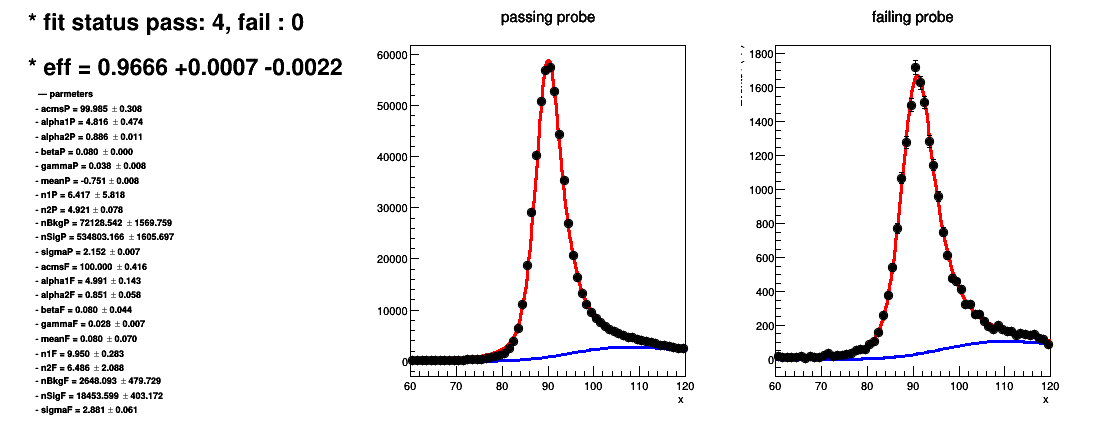
\includegraphics[height=0.355\textheight]{fits/wNF/seed_EE_R9gt0p93_et50.png}\\[2pt]
  \vspace{-10pt}\hfill\hyperlink{eff-seed-EE}{\beamerreturnbutton{efficiency}}
\end{frame}

\begin{frame}[label=fit-seed-EE-R9gt0p93-60]{Fits: seeded leg, EE $\RNine>0.93$, $60<\ET<70$~GeV}
  \centering
  {\scriptsize\hl{without NF}}\\[1pt]
  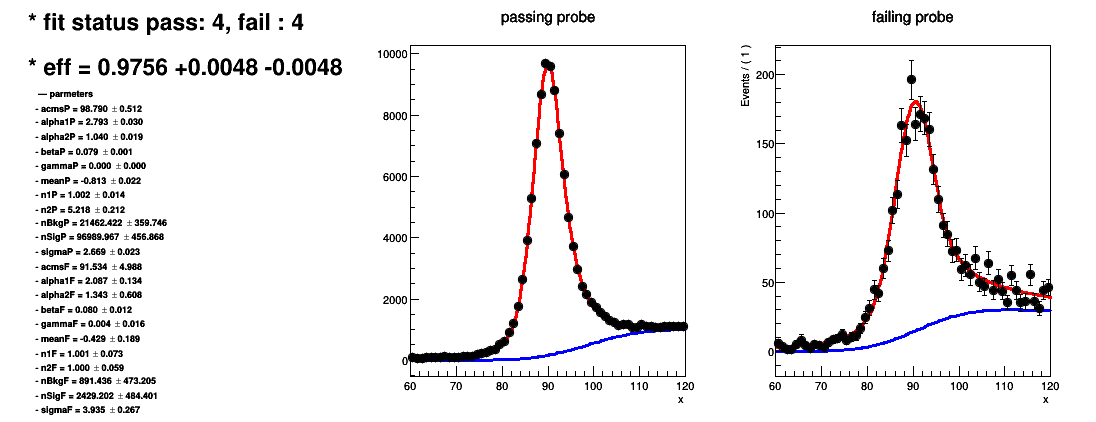
\includegraphics[height=0.355\textheight]{fits/woNF/seed_EE_R9gt0p93_et60.png}\\[2pt]
  {\scriptsize\hl{with NF}}\\[1pt]
  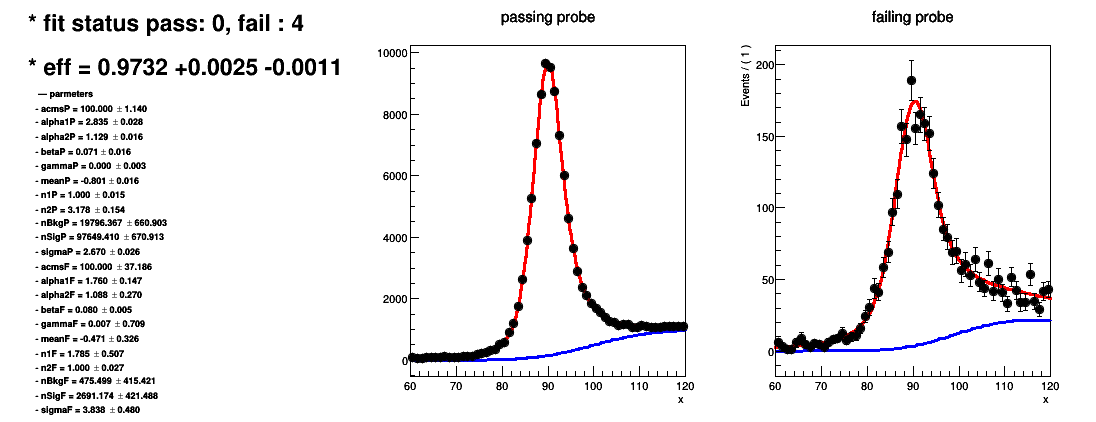
\includegraphics[height=0.355\textheight]{fits/wNF/seed_EE_R9gt0p93_et60.png}\\[2pt]
  \vspace{-10pt}\hfill\hyperlink{eff-seed-EE}{\beamerreturnbutton{efficiency}}
\end{frame}

\begin{frame}[label=fit-seed-EE-R9gt0p93-70]{Fits: seeded leg, EE $\RNine>0.93$, $70<\ET<90$~GeV}
  \centering
  {\scriptsize\hl{without NF}}\\[1pt]
  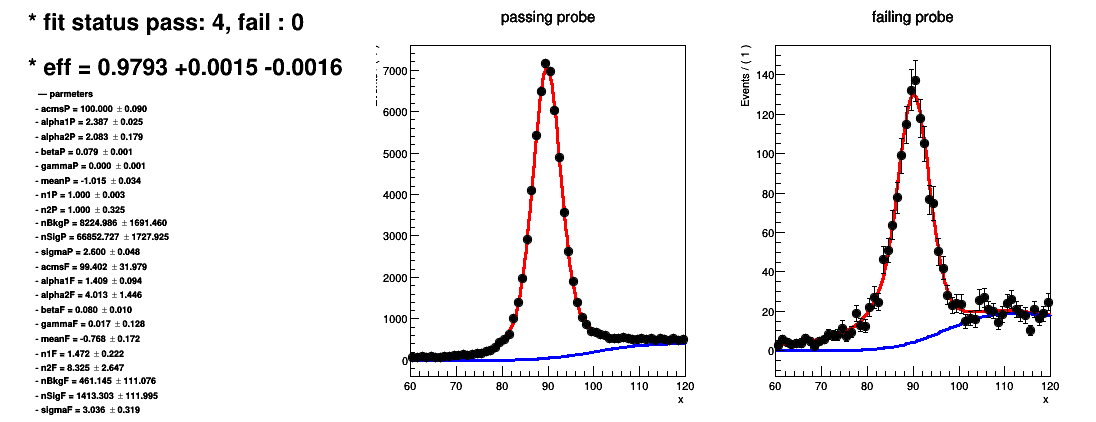
\includegraphics[height=0.355\textheight]{fits/woNF/seed_EE_R9gt0p93_et70.png}\\[2pt]
  {\scriptsize\hl{with NF}}\\[1pt]
  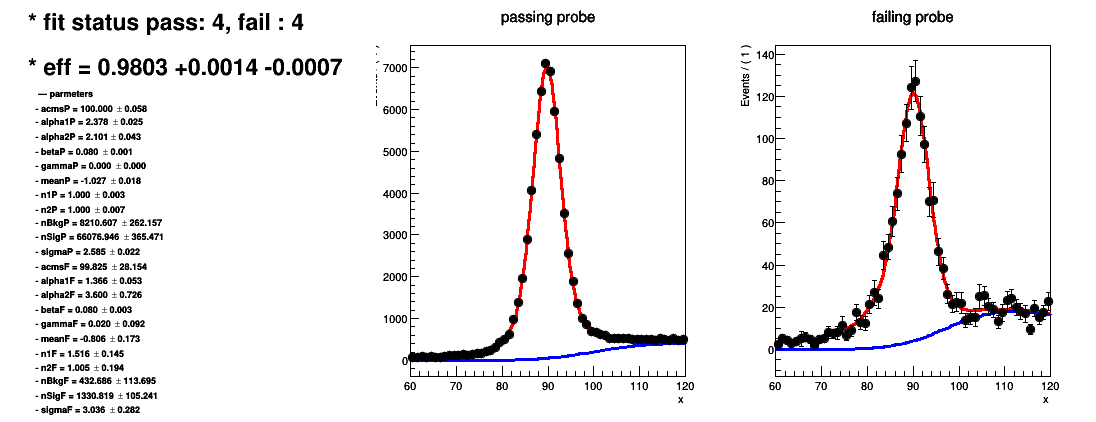
\includegraphics[height=0.355\textheight]{fits/wNF/seed_EE_R9gt0p93_et70.png}\\[2pt]
  \vspace{-10pt}\hfill\hyperlink{eff-seed-EE}{\beamerreturnbutton{efficiency}}
\end{frame}

\begin{frame}[label=fit-seed-EE-R9gt0p93-90]{Fits: seeded leg, EE $\RNine>0.93$, $\ET>90$~GeV}
  \centering
  {\scriptsize\hl{without NF}}\\[1pt]
  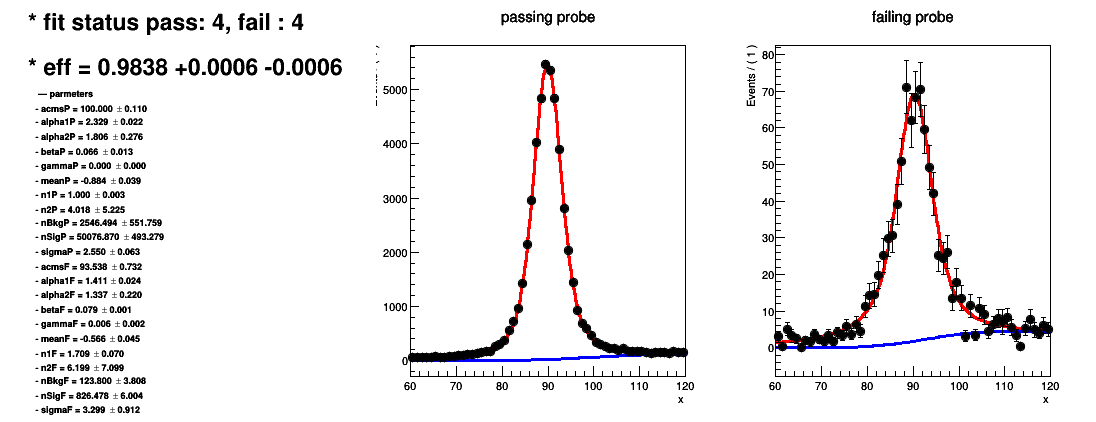
\includegraphics[height=0.355\textheight]{fits/woNF/seed_EE_R9gt0p93_et90.png}\\[2pt]
  {\scriptsize\hl{with NF}}\\[1pt]
  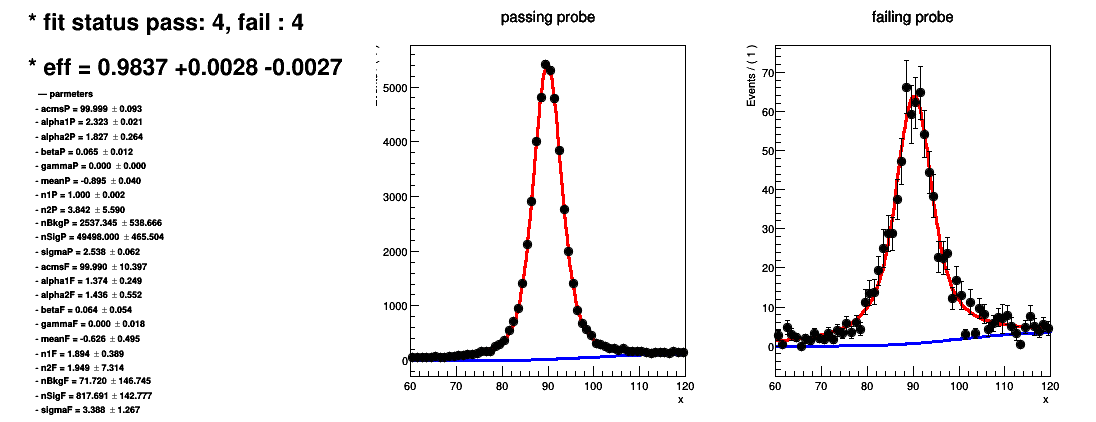
\includegraphics[height=0.355\textheight]{fits/wNF/seed_EE_R9gt0p93_et90.png}\\[2pt]
  \vspace{-10pt}\hfill\hyperlink{eff-seed-EE}{\beamerreturnbutton{efficiency}}
\end{frame}

\begin{frame}[label=fit-unseed-EB-R9-0p50to0p55-0]{Fits: unseeded leg, EB $0.50<\RNine<0.55$, $0<\ET<21$~GeV}
  \centering
  {\scriptsize\hl{without NF}}\\[1pt]
  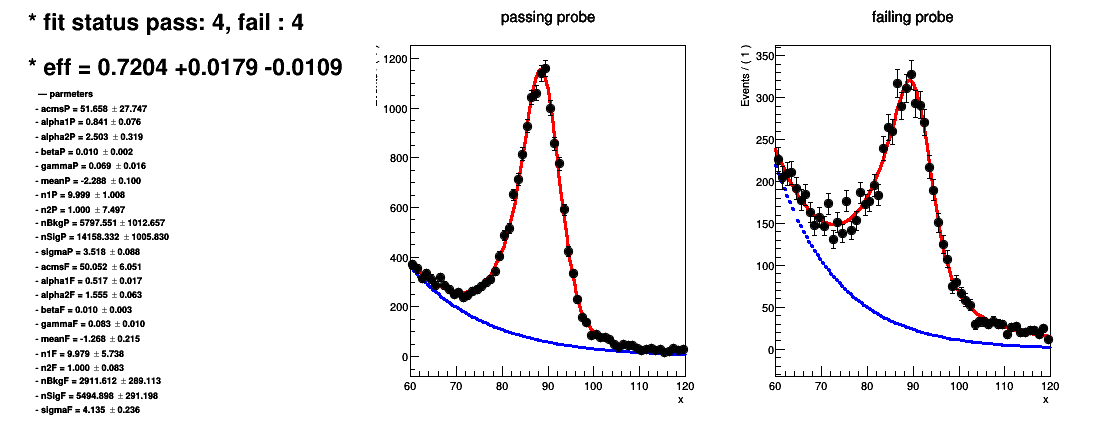
\includegraphics[height=0.355\textheight]{fits/woNF/unseed_EB_R9_0p50to0p55_et0.png}\\[2pt]
  {\scriptsize\hl{with NF}}\\[1pt]
  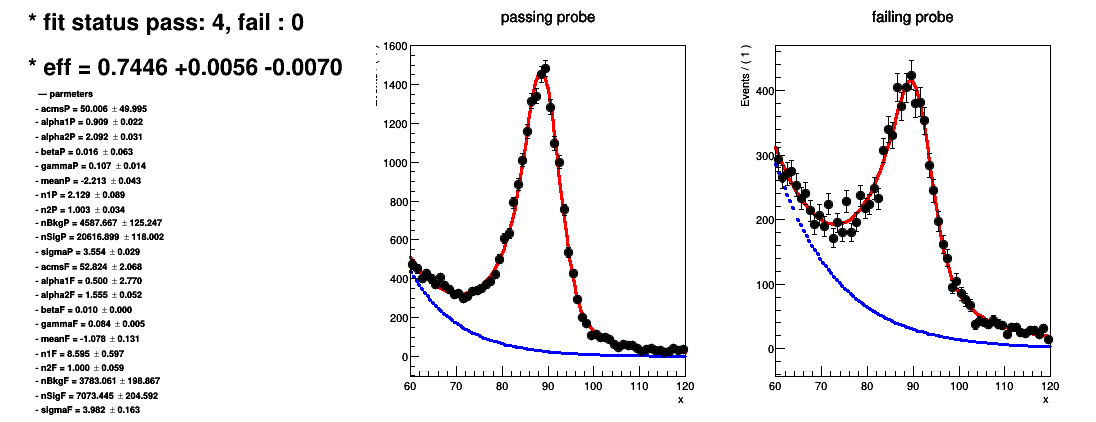
\includegraphics[height=0.355\textheight]{fits/wNF/unseed_EB_R9_0p50to0p55_et0.png}\\[2pt]
  \vspace{-10pt}\hfill\hyperlink{eff-unseed-EB}{\beamerreturnbutton{efficiency}}
\end{frame}

\begin{frame}[label=fit-unseed-EB-R9-0p50to0p55-21]{Fits: unseeded leg, EB $0.50<\RNine<0.55$, $21<\ET<25$~GeV}
  \centering
  {\scriptsize\hl{without NF}}\\[1pt]
  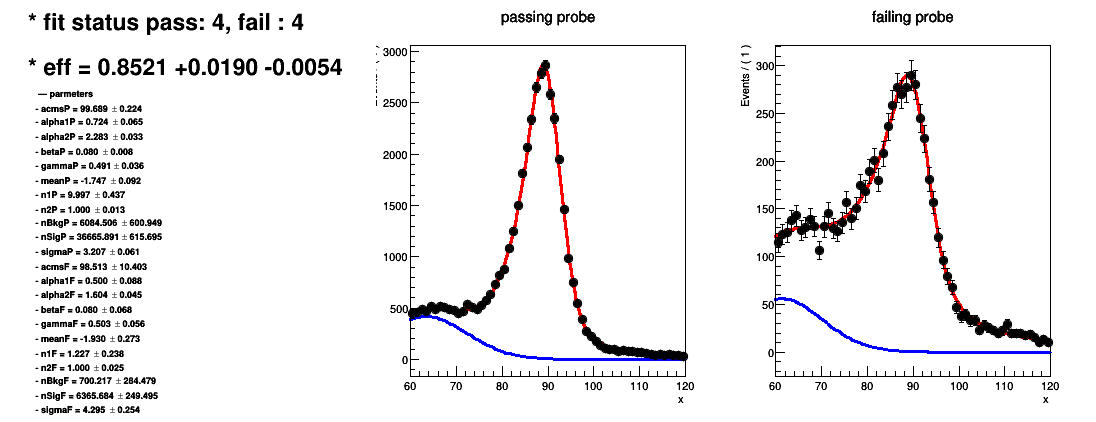
\includegraphics[height=0.355\textheight]{fits/woNF/unseed_EB_R9_0p50to0p55_et21.png}\\[2pt]
  {\scriptsize\hl{with NF}}\\[1pt]
  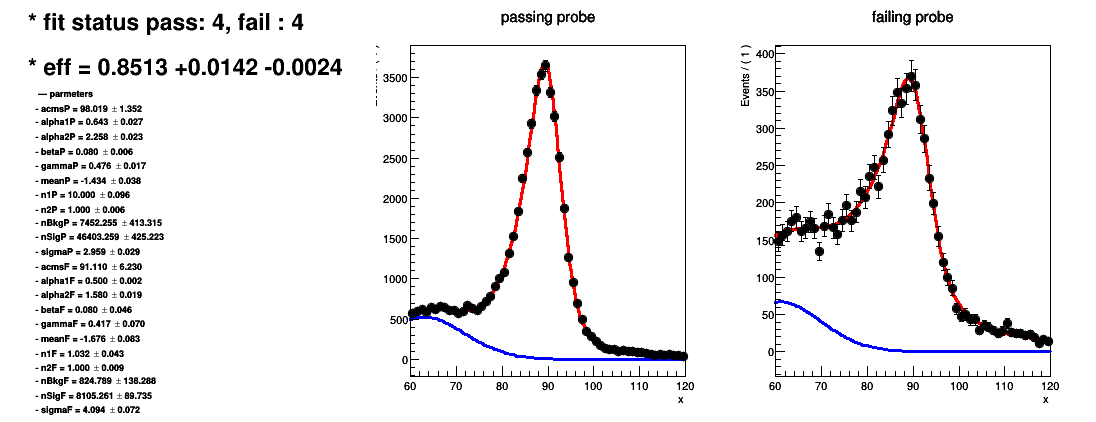
\includegraphics[height=0.355\textheight]{fits/wNF/unseed_EB_R9_0p50to0p55_et21.png}\\[2pt]
  \vspace{-10pt}\hfill\hyperlink{eff-unseed-EB}{\beamerreturnbutton{efficiency}}
\end{frame}

\begin{frame}[label=fit-unseed-EB-R9-0p50to0p55-25]{Fits: unseeded leg, EB $0.50<\RNine<0.55$, $25<\ET<28$~GeV}
  \centering
  {\scriptsize\hl{without NF}}\\[1pt]
  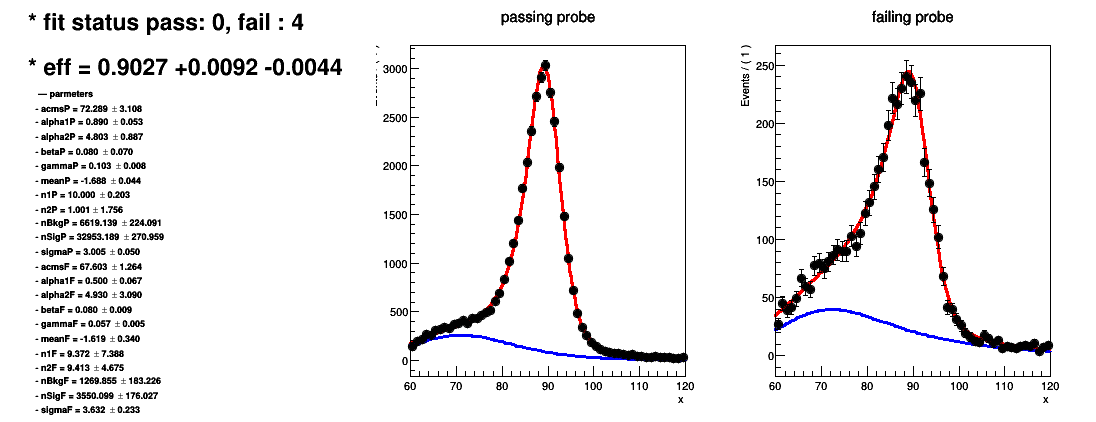
\includegraphics[height=0.355\textheight]{fits/woNF/unseed_EB_R9_0p50to0p55_et25.png}\\[2pt]
  {\scriptsize\hl{with NF}}\\[1pt]
  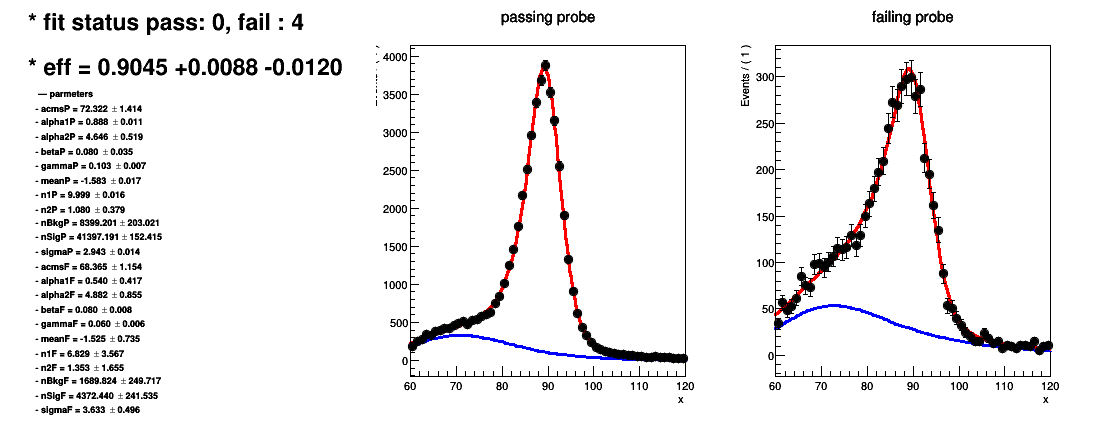
\includegraphics[height=0.355\textheight]{fits/wNF/unseed_EB_R9_0p50to0p55_et25.png}\\[2pt]
  \vspace{-10pt}\hfill\hyperlink{eff-unseed-EB}{\beamerreturnbutton{efficiency}}
\end{frame}

\begin{frame}[label=fit-unseed-EB-R9-0p50to0p55-28]{Fits: unseeded leg, EB $0.50<\RNine<0.55$, $28<\ET<31$~GeV}
  \centering
  {\scriptsize\hl{without NF}}\\[1pt]
  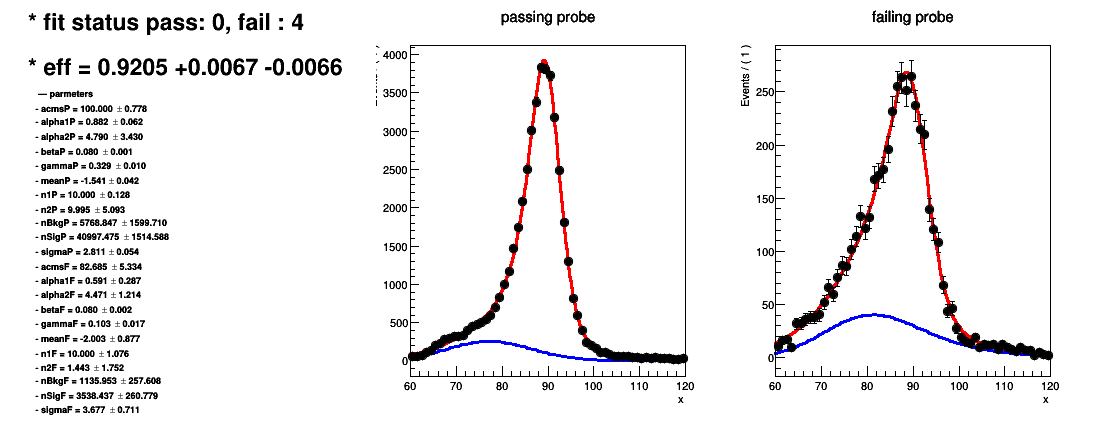
\includegraphics[height=0.355\textheight]{fits/woNF/unseed_EB_R9_0p50to0p55_et28.png}\\[2pt]
  {\scriptsize\hl{with NF}}\\[1pt]
  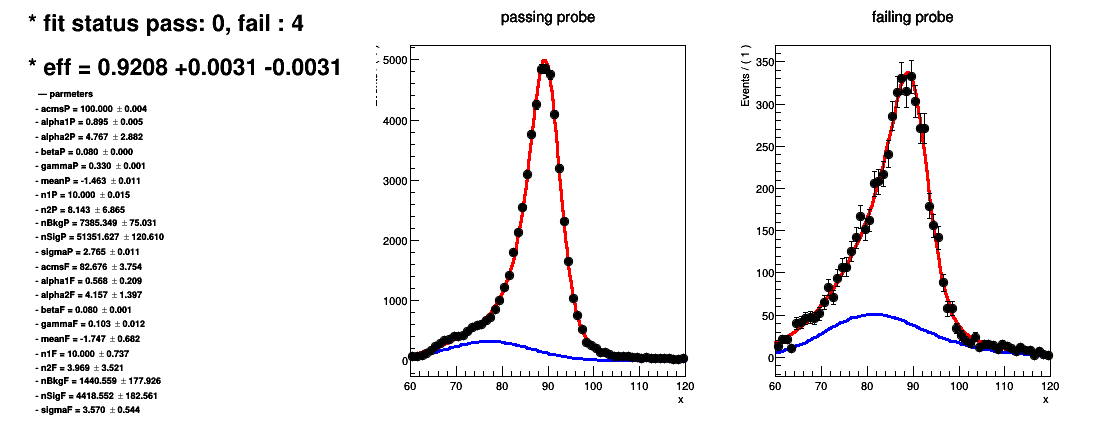
\includegraphics[height=0.355\textheight]{fits/wNF/unseed_EB_R9_0p50to0p55_et28.png}\\[2pt]
  \vspace{-10pt}\hfill\hyperlink{eff-unseed-EB}{\beamerreturnbutton{efficiency}}
\end{frame}

\begin{frame}[label=fit-unseed-EB-R9-0p50to0p55-31]{Fits: unseeded leg, EB $0.50<\RNine<0.55$, $31<\ET<35$~GeV}
  \centering
  {\scriptsize\hl{without NF}}\\[1pt]
  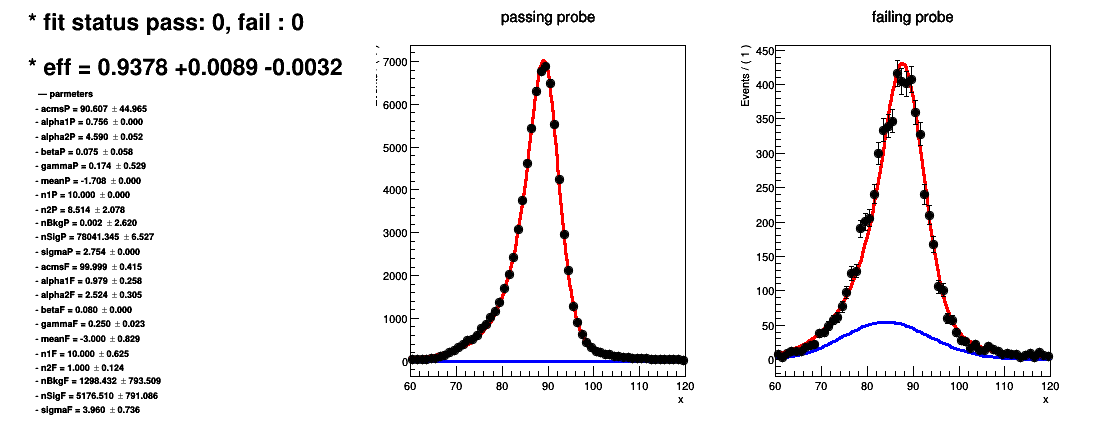
\includegraphics[height=0.355\textheight]{fits/woNF/unseed_EB_R9_0p50to0p55_et31.png}\\[2pt]
  {\scriptsize\hl{with NF}}\\[1pt]
  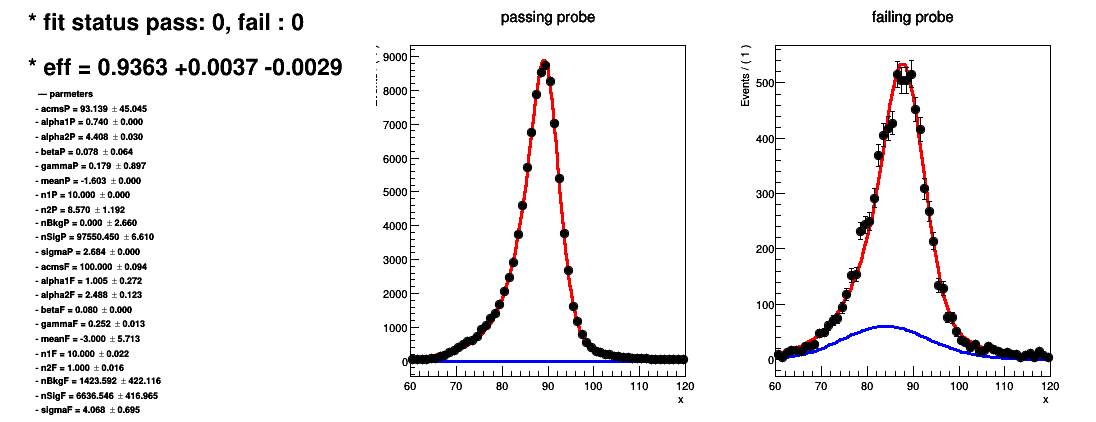
\includegraphics[height=0.355\textheight]{fits/wNF/unseed_EB_R9_0p50to0p55_et31.png}\\[2pt]
  \vspace{-10pt}\hfill\hyperlink{eff-unseed-EB}{\beamerreturnbutton{efficiency}}
\end{frame}

\begin{frame}[label=fit-unseed-EB-R9-0p50to0p55-35]{Fits: unseeded leg, EB $0.50<\RNine<0.55$, $35<\ET<40$~GeV}
  \centering
  {\scriptsize\hl{without NF}}\\[1pt]
  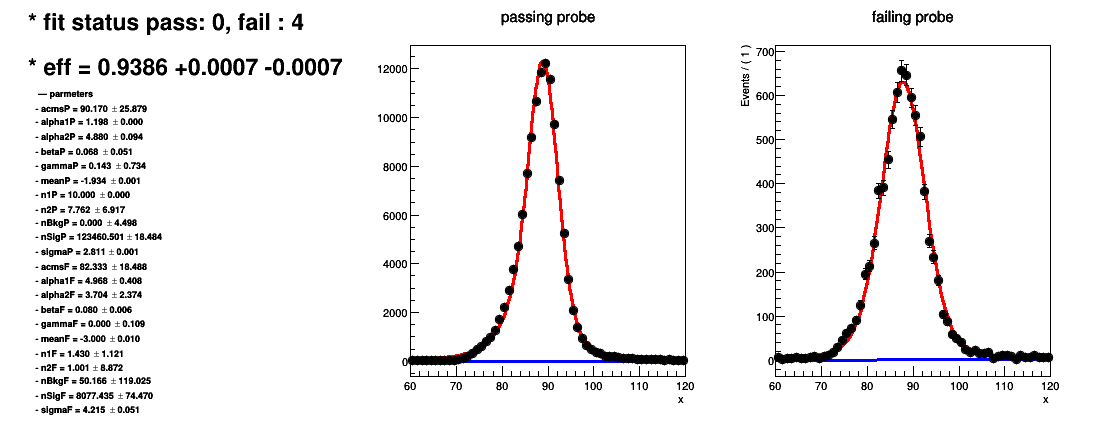
\includegraphics[height=0.355\textheight]{fits/woNF/unseed_EB_R9_0p50to0p55_et35.png}\\[2pt]
  {\scriptsize\hl{with NF}}\\[1pt]
  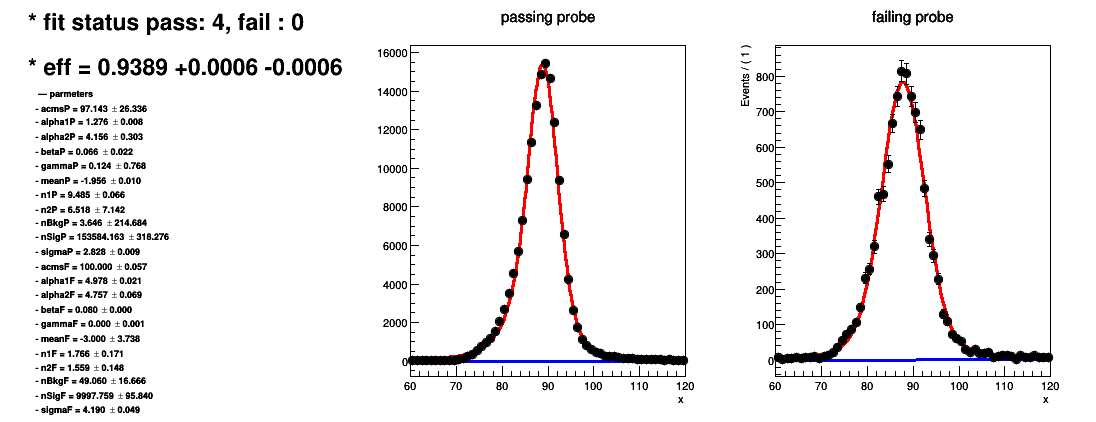
\includegraphics[height=0.355\textheight]{fits/wNF/unseed_EB_R9_0p50to0p55_et35.png}\\[2pt]
  \vspace{-10pt}\hfill\hyperlink{eff-unseed-EB}{\beamerreturnbutton{efficiency}}
\end{frame}

\begin{frame}[label=fit-unseed-EB-R9-0p50to0p55-40]{Fits: unseeded leg, EB $0.50<\RNine<0.55$, $40<\ET<45$~GeV}
  \centering
  {\scriptsize\hl{without NF}}\\[1pt]
  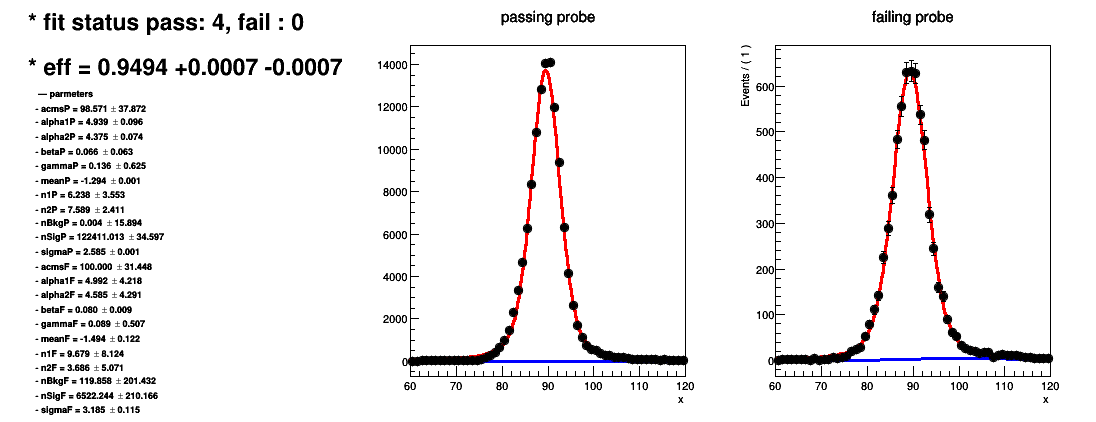
\includegraphics[height=0.355\textheight]{fits/woNF/unseed_EB_R9_0p50to0p55_et40.png}\\[2pt]
  {\scriptsize\hl{with NF}}\\[1pt]
  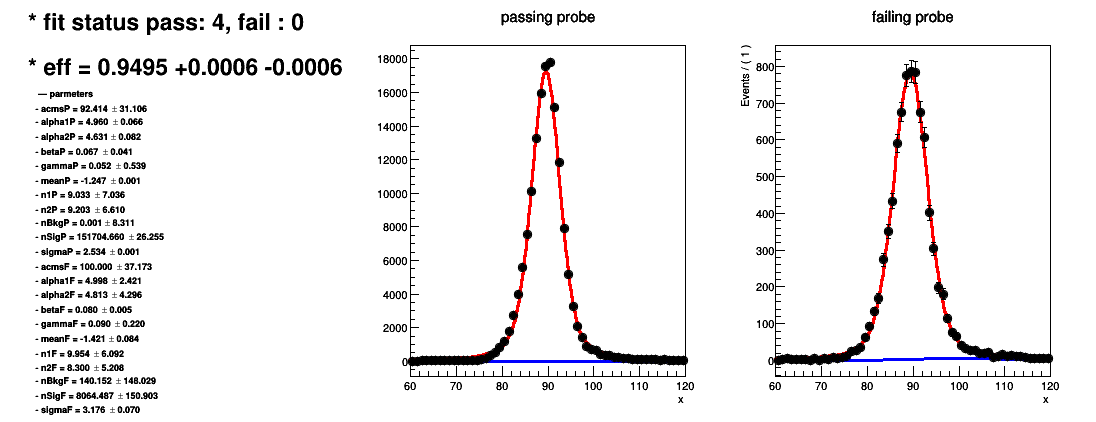
\includegraphics[height=0.355\textheight]{fits/wNF/unseed_EB_R9_0p50to0p55_et40.png}\\[2pt]
  \vspace{-10pt}\hfill\hyperlink{eff-unseed-EB}{\beamerreturnbutton{efficiency}}
\end{frame}

\begin{frame}[label=fit-unseed-EB-R9-0p50to0p55-45]{Fits: unseeded leg, EB $0.50<\RNine<0.55$, $45<\ET<50$~GeV}
  \centering
  {\scriptsize\hl{without NF}}\\[1pt]
  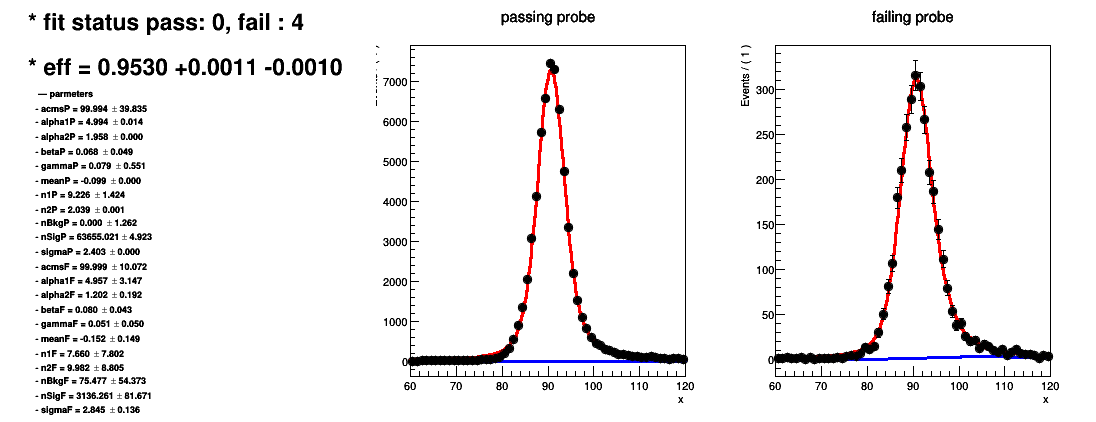
\includegraphics[height=0.355\textheight]{fits/woNF/unseed_EB_R9_0p50to0p55_et45.png}\\[2pt]
  {\scriptsize\hl{with NF}}\\[1pt]
  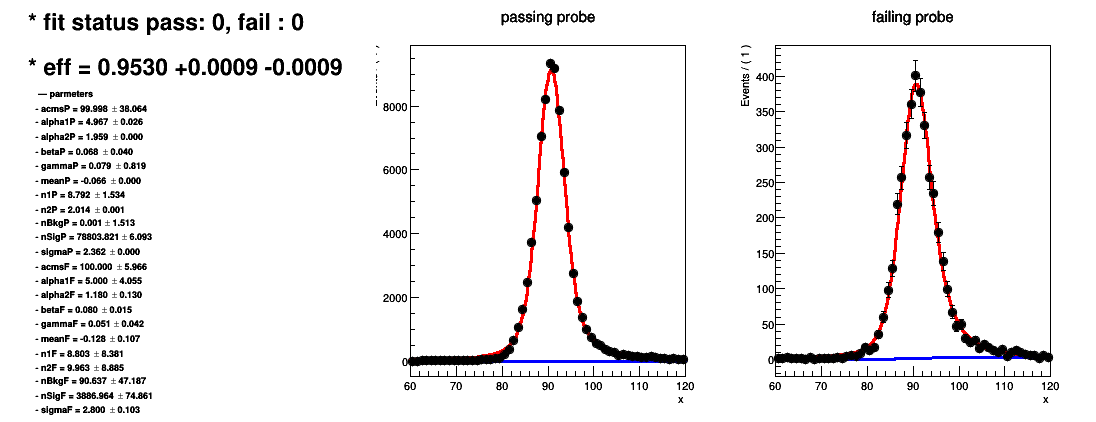
\includegraphics[height=0.355\textheight]{fits/wNF/unseed_EB_R9_0p50to0p55_et45.png}\\[2pt]
  \vspace{-10pt}\hfill\hyperlink{eff-unseed-EB}{\beamerreturnbutton{efficiency}}
\end{frame}

\begin{frame}[label=fit-unseed-EB-R9-0p50to0p55-50]{Fits: unseeded leg, EB $0.50<\RNine<0.55$, $50<\ET<60$~GeV}
  \centering
  {\scriptsize\hl{without NF}}\\[1pt]
  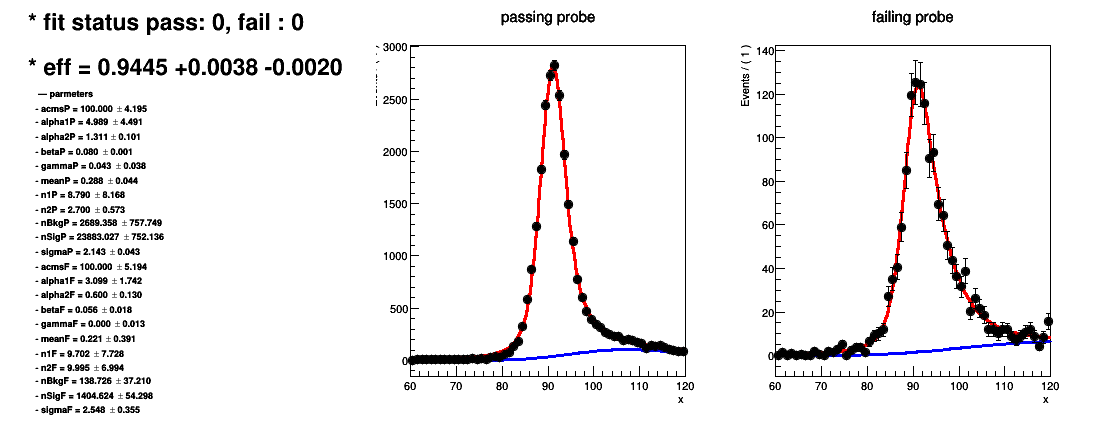
\includegraphics[height=0.355\textheight]{fits/woNF/unseed_EB_R9_0p50to0p55_et50.png}\\[2pt]
  {\scriptsize\hl{with NF}}\\[1pt]
  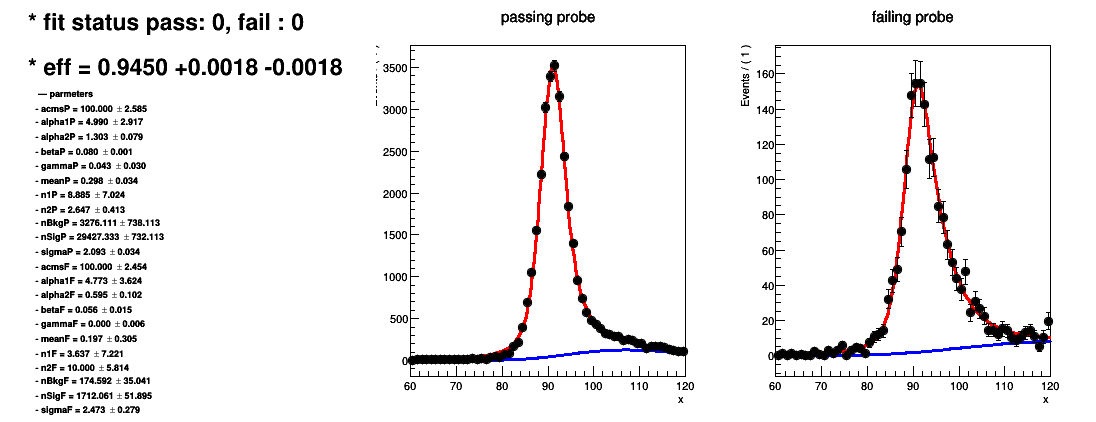
\includegraphics[height=0.355\textheight]{fits/wNF/unseed_EB_R9_0p50to0p55_et50.png}\\[2pt]
  \vspace{-10pt}\hfill\hyperlink{eff-unseed-EB}{\beamerreturnbutton{efficiency}}
\end{frame}

\begin{frame}[label=fit-unseed-EB-R9-0p50to0p55-60]{Fits: unseeded leg, EB $0.50<\RNine<0.55$, $60<\ET<70$~GeV}
  \centering
  {\scriptsize\hl{without NF}}\\[1pt]
  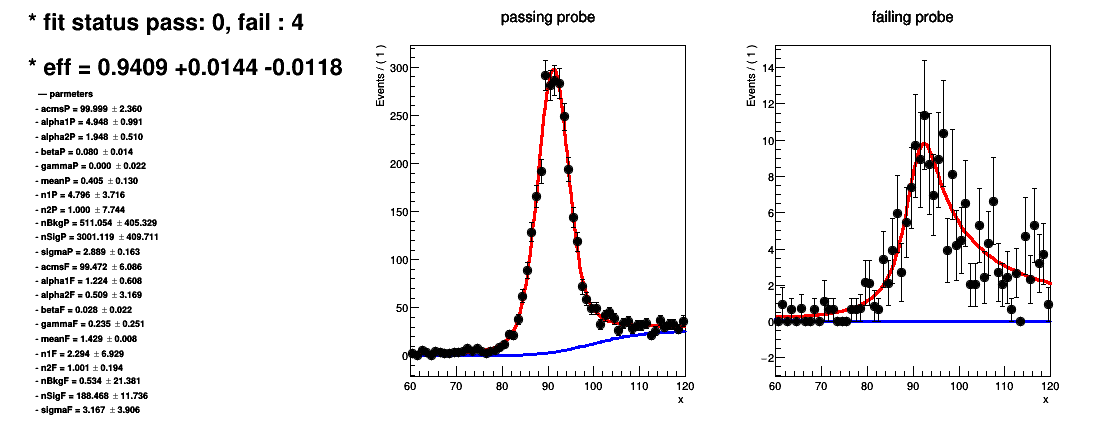
\includegraphics[height=0.355\textheight]{fits/woNF/unseed_EB_R9_0p50to0p55_et60.png}\\[2pt]
  {\scriptsize\hl{with NF}}\\[1pt]
  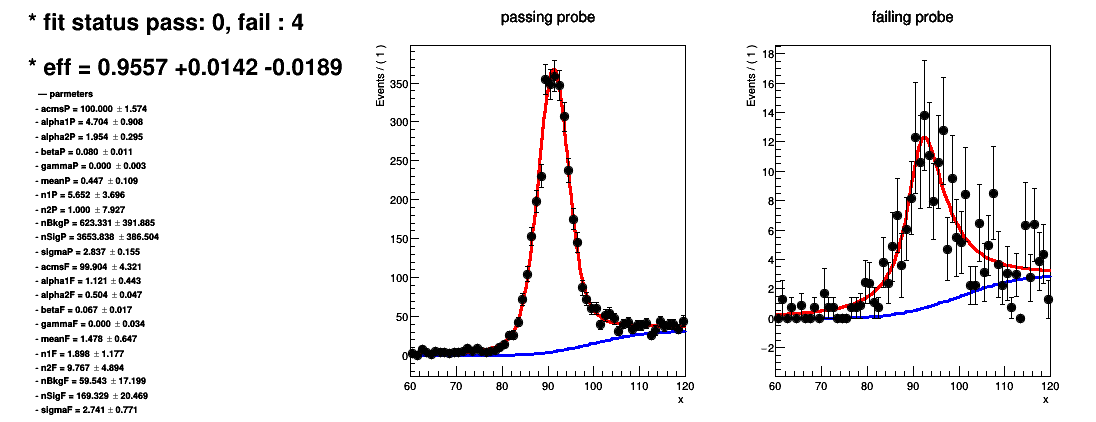
\includegraphics[height=0.355\textheight]{fits/wNF/unseed_EB_R9_0p50to0p55_et60.png}\\[2pt]
  \vspace{-10pt}\hfill\hyperlink{eff-unseed-EB}{\beamerreturnbutton{efficiency}}
\end{frame}

\begin{frame}[label=fit-unseed-EB-R9-0p50to0p55-70]{Fits: unseeded leg, EB $0.50<\RNine<0.55$, $70<\ET<90$~GeV}
  \centering
  {\scriptsize\hl{without NF}}\\[1pt]
  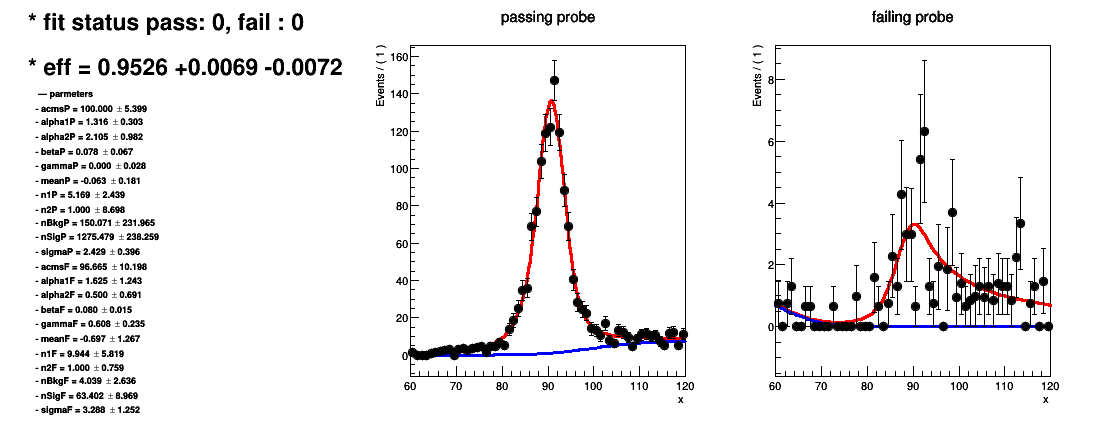
\includegraphics[height=0.355\textheight]{fits/woNF/unseed_EB_R9_0p50to0p55_et70.png}\\[2pt]
  {\scriptsize\hl{with NF}}\\[1pt]
  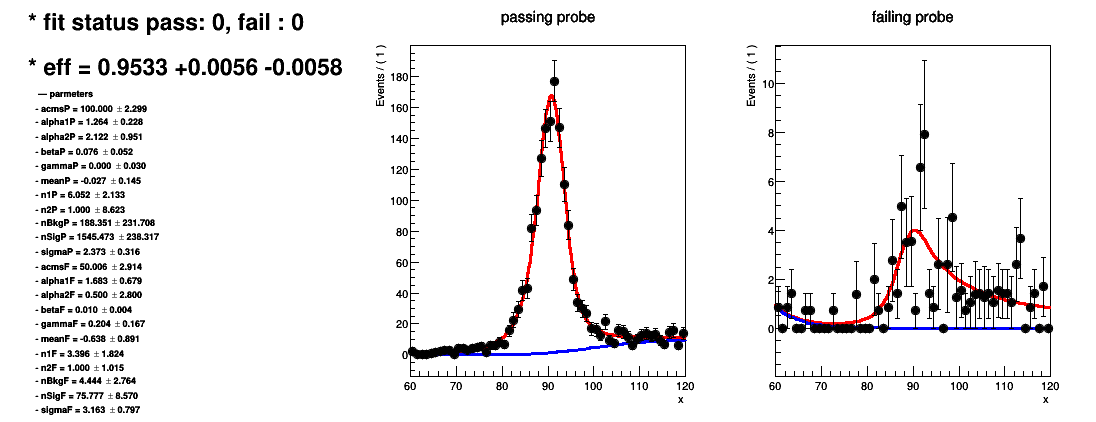
\includegraphics[height=0.355\textheight]{fits/wNF/unseed_EB_R9_0p50to0p55_et70.png}\\[2pt]
  \vspace{-10pt}\hfill\hyperlink{eff-unseed-EB}{\beamerreturnbutton{efficiency}}
\end{frame}

\begin{frame}[label=fit-unseed-EB-R9-0p50to0p55-90]{Fits: unseeded leg, EB $0.50<\RNine<0.55$, $\ET>90$~GeV}
  \centering
  {\scriptsize\hl{without NF}}\\[1pt]
  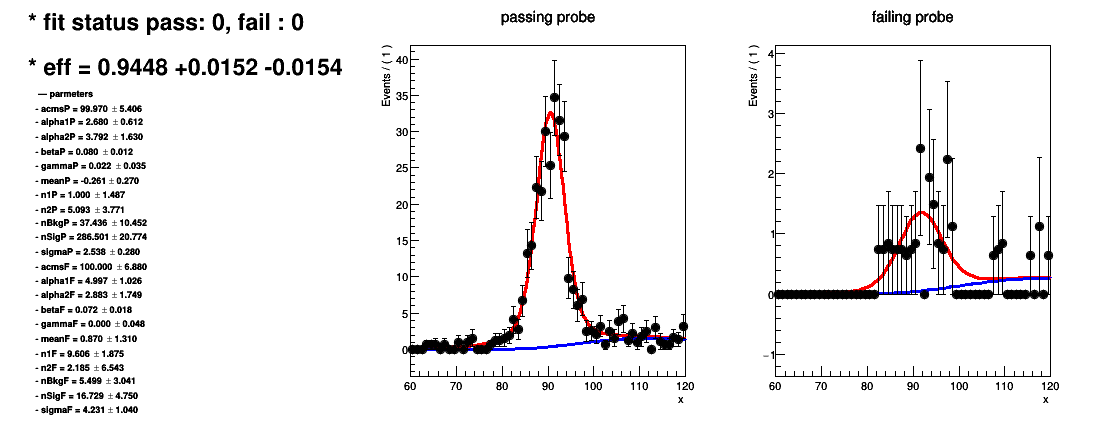
\includegraphics[height=0.355\textheight]{fits/woNF/unseed_EB_R9_0p50to0p55_et90.png}\\[2pt]
  {\scriptsize\hl{with NF}}\\[1pt]
  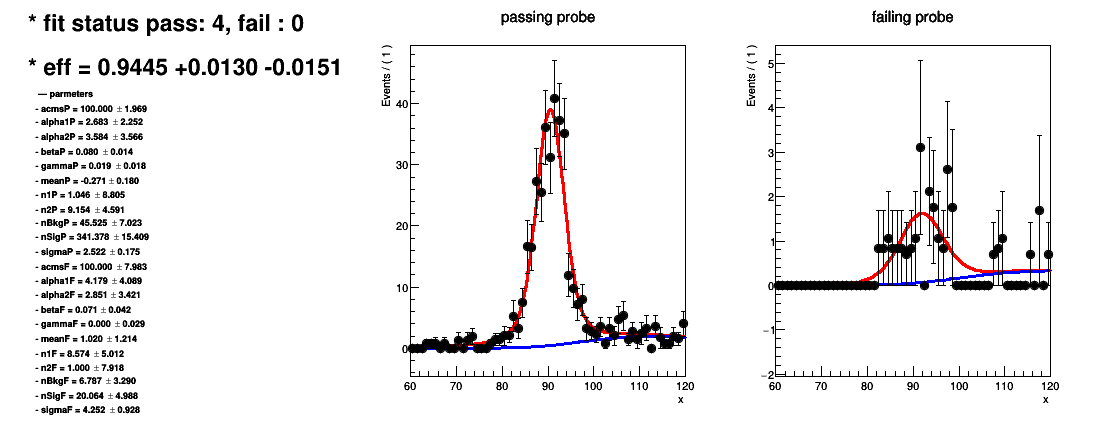
\includegraphics[height=0.355\textheight]{fits/wNF/unseed_EB_R9_0p50to0p55_et90.png}\\[2pt]
  \vspace{-10pt}\hfill\hyperlink{eff-unseed-EB}{\beamerreturnbutton{efficiency}}
\end{frame}

\begin{frame}[label=fit-unseed-EB-R9-0p55to0p85-0]{Fits: unseeded leg, EB $0.55<\RNine<0.85$, $0<\ET<21$~GeV}
  \centering
  {\scriptsize\hl{without NF}}\\[1pt]
  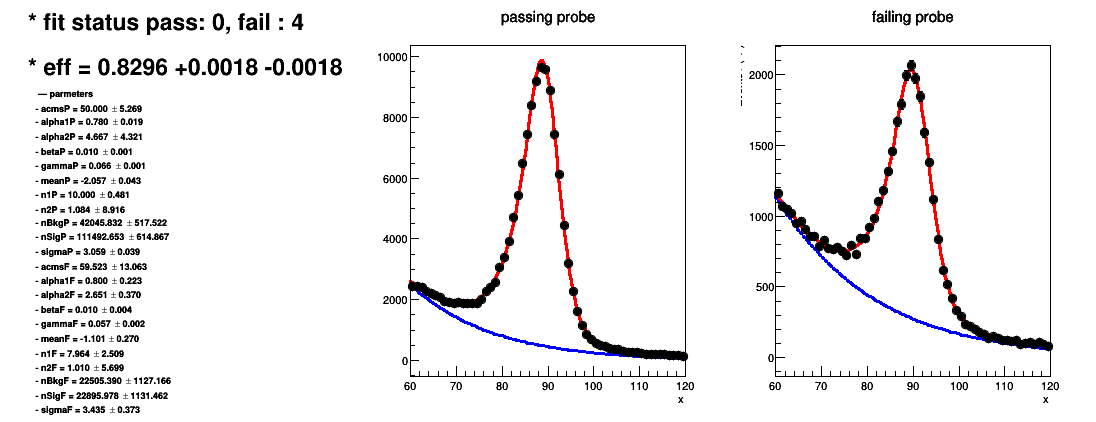
\includegraphics[height=0.355\textheight]{fits/woNF/unseed_EB_R9_0p55to0p85_et0.png}\\[2pt]
  {\scriptsize\hl{with NF}}\\[1pt]
  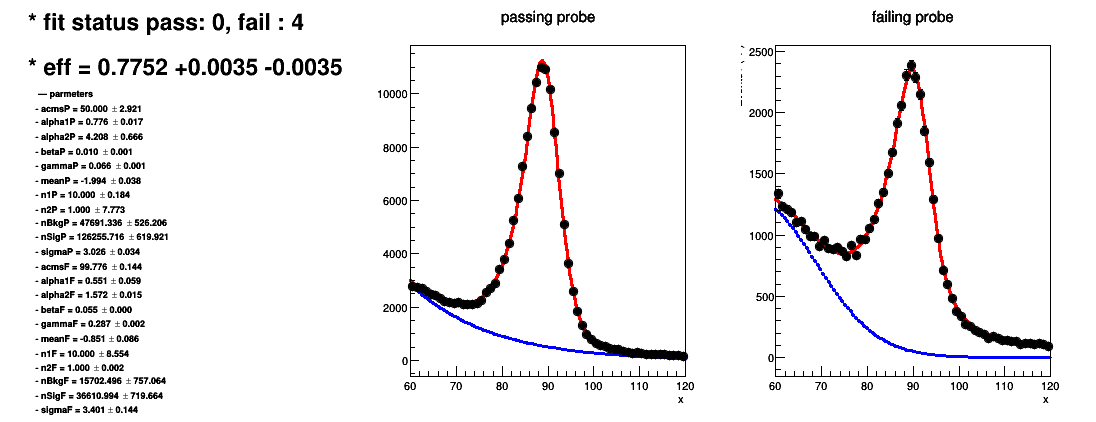
\includegraphics[height=0.355\textheight]{fits/wNF/unseed_EB_R9_0p55to0p85_et0.png}\\[2pt]
  \vspace{-10pt}\hfill\hyperlink{eff-unseed-EB}{\beamerreturnbutton{efficiency}}
\end{frame}

\begin{frame}[label=fit-unseed-EB-R9-0p55to0p85-21]{Fits: unseeded leg, EB $0.55<\RNine<0.85$, $21<\ET<25$~GeV}
  \centering
  {\scriptsize\hl{without NF}}\\[1pt]
  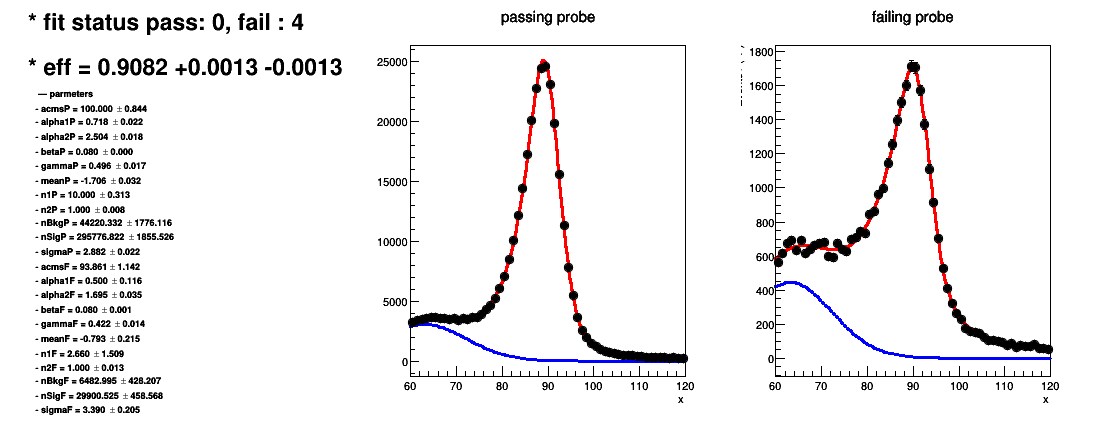
\includegraphics[height=0.355\textheight]{fits/woNF/unseed_EB_R9_0p55to0p85_et21.png}\\[2pt]
  {\scriptsize\hl{with NF}}\\[1pt]
  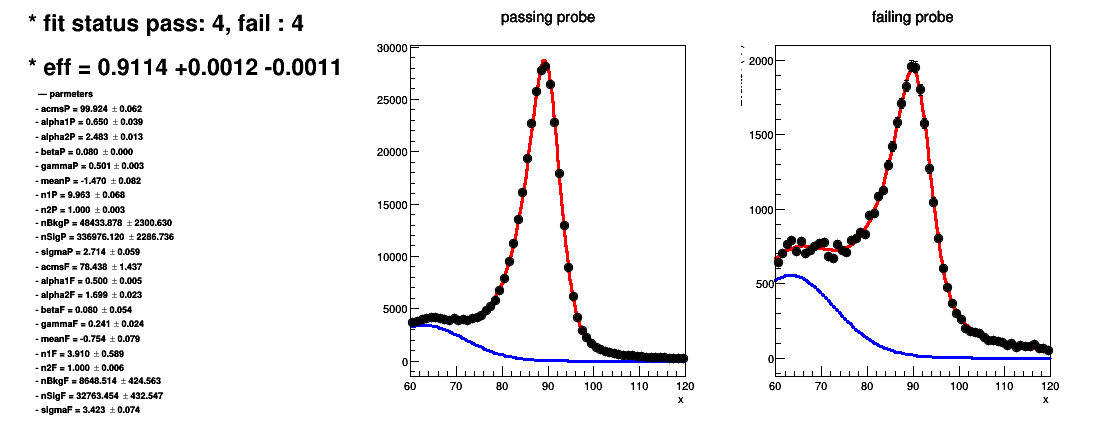
\includegraphics[height=0.355\textheight]{fits/wNF/unseed_EB_R9_0p55to0p85_et21.png}\\[2pt]
  \vspace{-10pt}\hfill\hyperlink{eff-unseed-EB}{\beamerreturnbutton{efficiency}}
\end{frame}

\begin{frame}[label=fit-unseed-EB-R9-0p55to0p85-25]{Fits: unseeded leg, EB $0.55<\RNine<0.85$, $25<\ET<28$~GeV}
  \centering
  {\scriptsize\hl{without NF}}\\[1pt]
  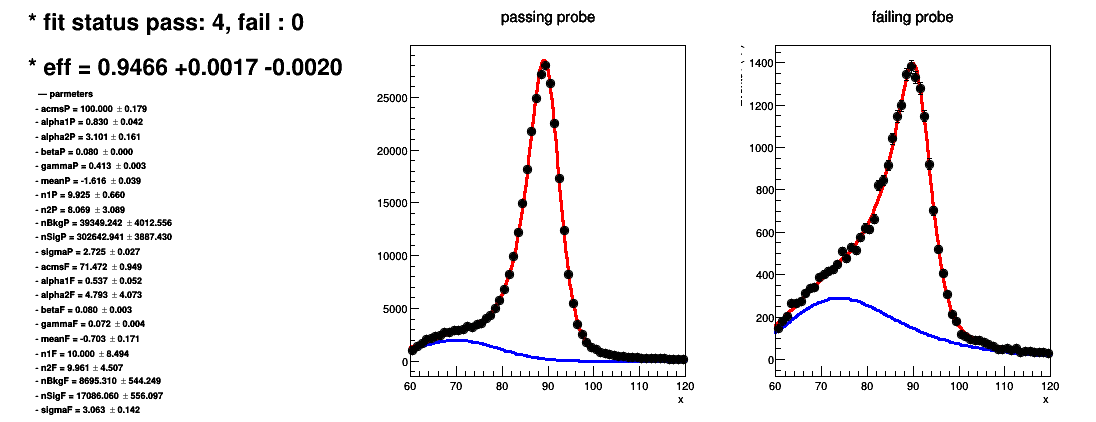
\includegraphics[height=0.355\textheight]{fits/woNF/unseed_EB_R9_0p55to0p85_et25.png}\\[2pt]
  {\scriptsize\hl{with NF}}\\[1pt]
  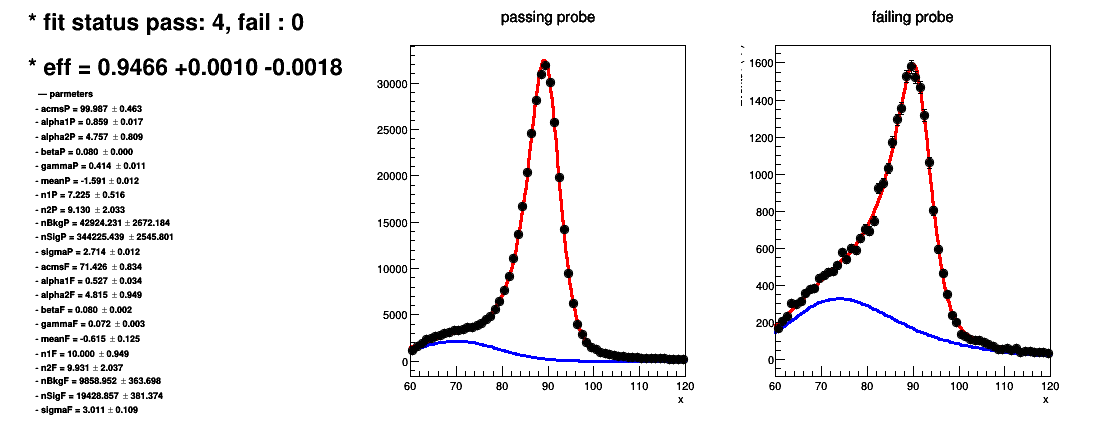
\includegraphics[height=0.355\textheight]{fits/wNF/unseed_EB_R9_0p55to0p85_et25.png}\\[2pt]
  \vspace{-10pt}\hfill\hyperlink{eff-unseed-EB}{\beamerreturnbutton{efficiency}}
\end{frame}

\begin{frame}[label=fit-unseed-EB-R9-0p55to0p85-28]{Fits: unseeded leg, EB $0.55<\RNine<0.85$, $28<\ET<31$~GeV}
  \centering
  {\scriptsize\hl{without NF}}\\[1pt]
  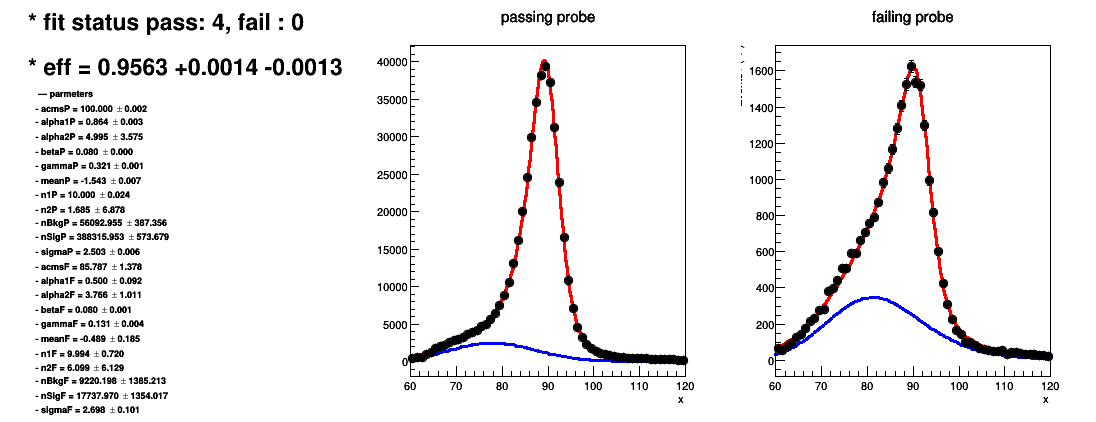
\includegraphics[height=0.355\textheight]{fits/woNF/unseed_EB_R9_0p55to0p85_et28.png}\\[2pt]
  {\scriptsize\hl{with NF}}\\[1pt]
  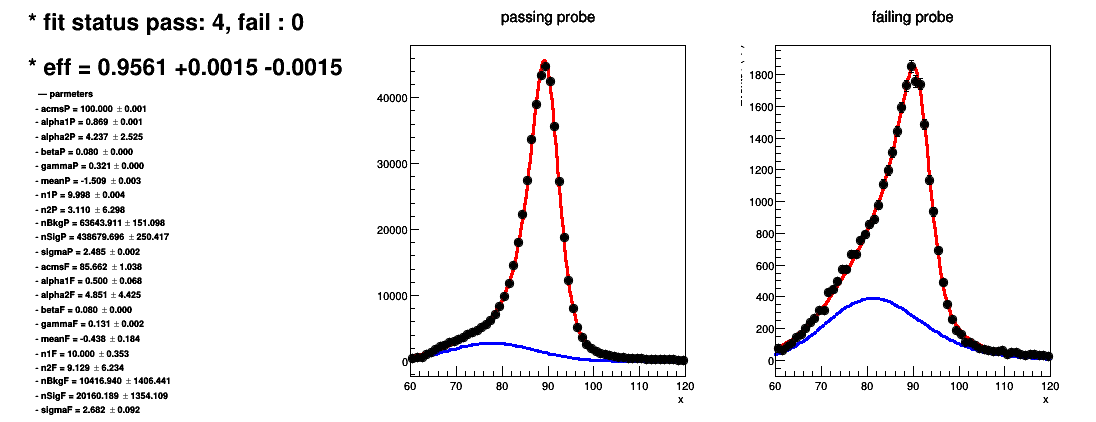
\includegraphics[height=0.355\textheight]{fits/wNF/unseed_EB_R9_0p55to0p85_et28.png}\\[2pt]
  \vspace{-10pt}\hfill\hyperlink{eff-unseed-EB}{\beamerreturnbutton{efficiency}}
\end{frame}

\begin{frame}[label=fit-unseed-EB-R9-0p55to0p85-31]{Fits: unseeded leg, EB $0.55<\RNine<0.85$, $31<\ET<35$~GeV}
  \centering
  {\scriptsize\hl{without NF}}\\[1pt]
  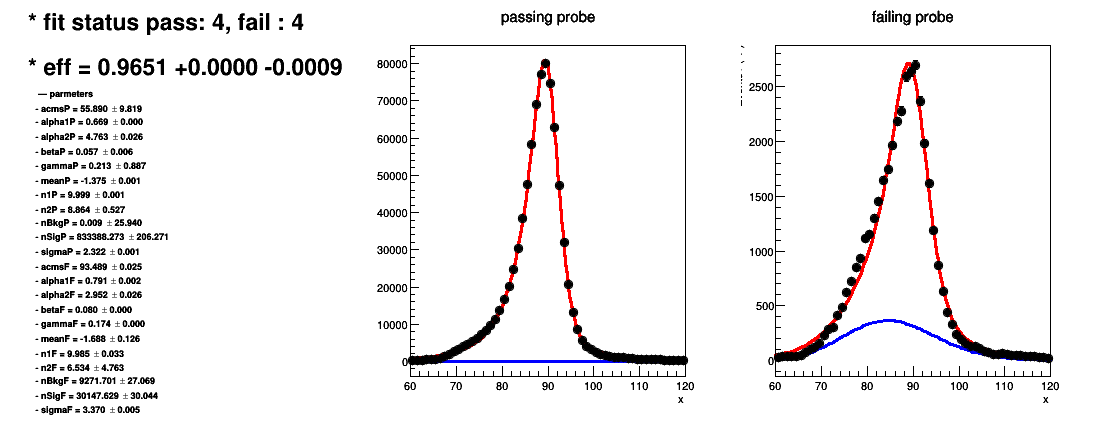
\includegraphics[height=0.355\textheight]{fits/woNF/unseed_EB_R9_0p55to0p85_et31.png}\\[2pt]
  {\scriptsize\hl{with NF}}\\[1pt]
  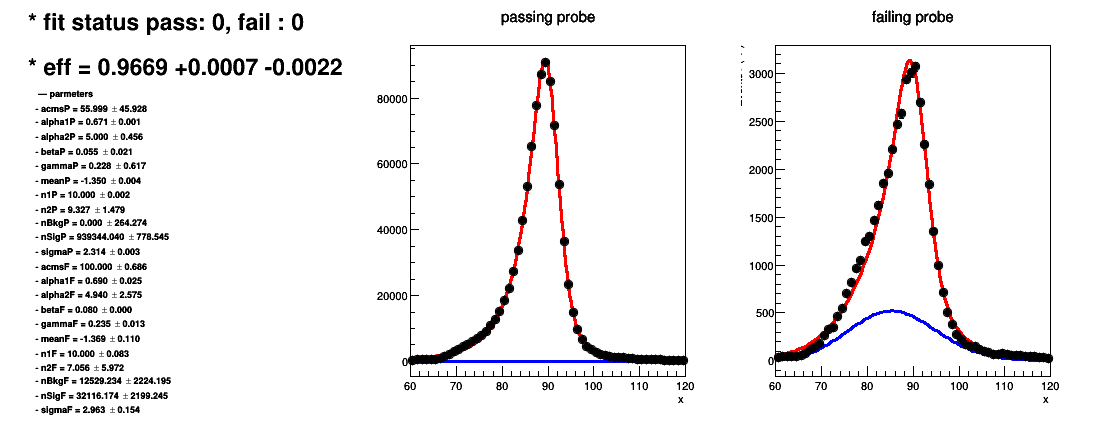
\includegraphics[height=0.355\textheight]{fits/wNF/unseed_EB_R9_0p55to0p85_et31.png}\\[2pt]
  \vspace{-10pt}\hfill\hyperlink{eff-unseed-EB}{\beamerreturnbutton{efficiency}}
\end{frame}

\begin{frame}[label=fit-unseed-EB-R9-0p55to0p85-35]{Fits: unseeded leg, EB $0.55<\RNine<0.85$, $35<\ET<40$~GeV}
  \centering
  {\scriptsize\hl{without NF}}\\[1pt]
  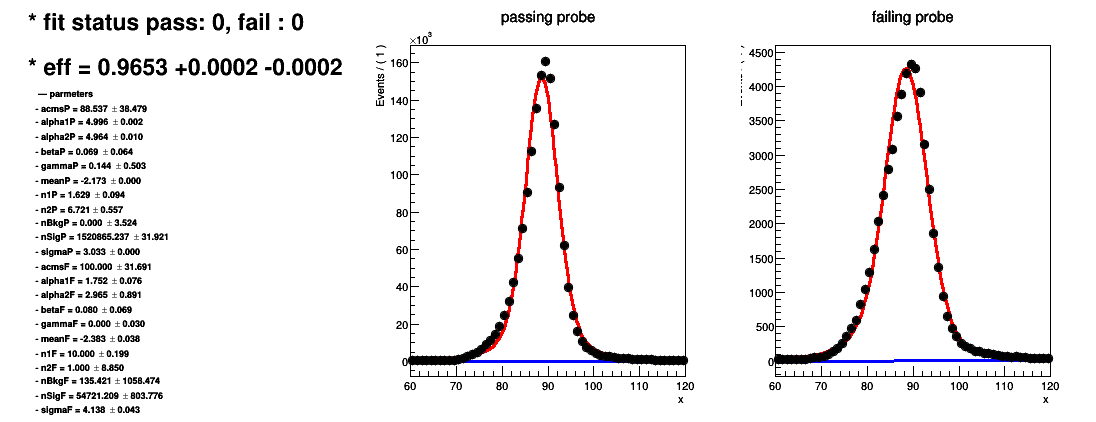
\includegraphics[height=0.355\textheight]{fits/woNF/unseed_EB_R9_0p55to0p85_et35.png}\\[2pt]
  {\scriptsize\hl{with NF}}\\[1pt]
  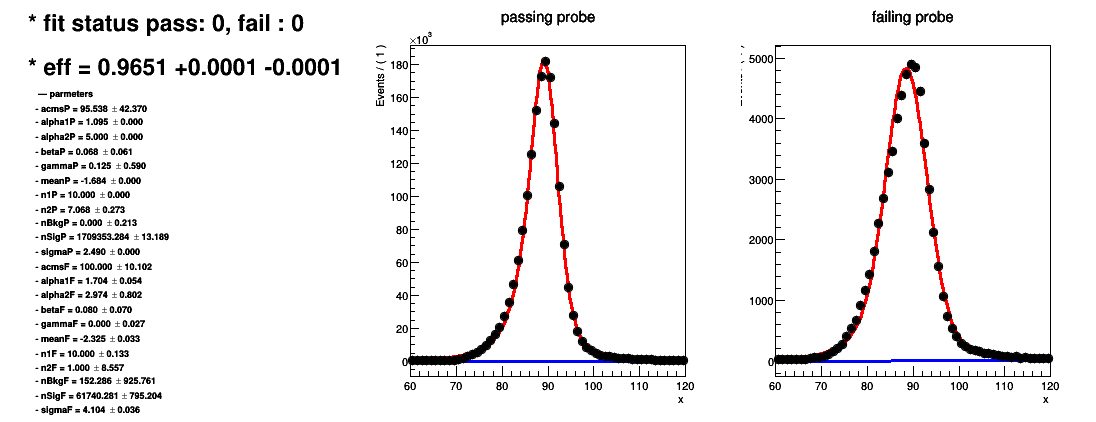
\includegraphics[height=0.355\textheight]{fits/wNF/unseed_EB_R9_0p55to0p85_et35.png}\\[2pt]
  \vspace{-10pt}\hfill\hyperlink{eff-unseed-EB}{\beamerreturnbutton{efficiency}}
\end{frame}

\begin{frame}[label=fit-unseed-EB-R9-0p55to0p85-40]{Fits: unseeded leg, EB $0.55<\RNine<0.85$, $40<\ET<45$~GeV}
  \centering
  {\scriptsize\hl{without NF}}\\[1pt]
  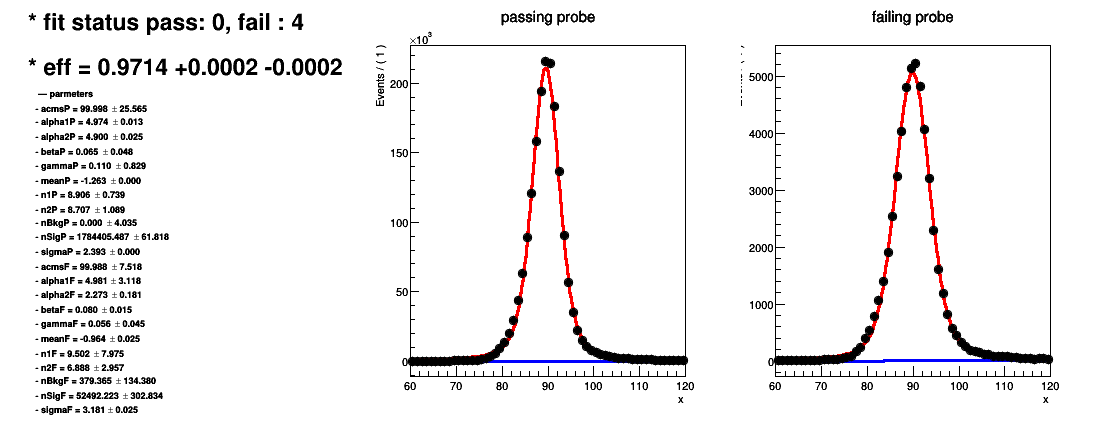
\includegraphics[height=0.355\textheight]{fits/woNF/unseed_EB_R9_0p55to0p85_et40.png}\\[2pt]
  {\scriptsize\hl{with NF}}\\[1pt]
  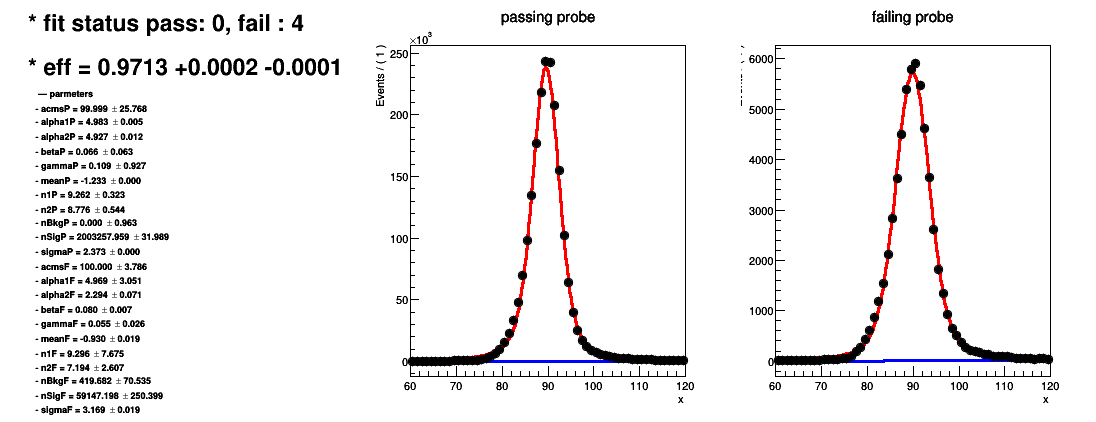
\includegraphics[height=0.355\textheight]{fits/wNF/unseed_EB_R9_0p55to0p85_et40.png}\\[2pt]
  \vspace{-10pt}\hfill\hyperlink{eff-unseed-EB}{\beamerreturnbutton{efficiency}}
\end{frame}

\begin{frame}[label=fit-unseed-EB-R9-0p55to0p85-45]{Fits: unseeded leg, EB $0.55<\RNine<0.85$, $45<\ET<50$~GeV}
  \centering
  {\scriptsize\hl{without NF}}\\[1pt]
  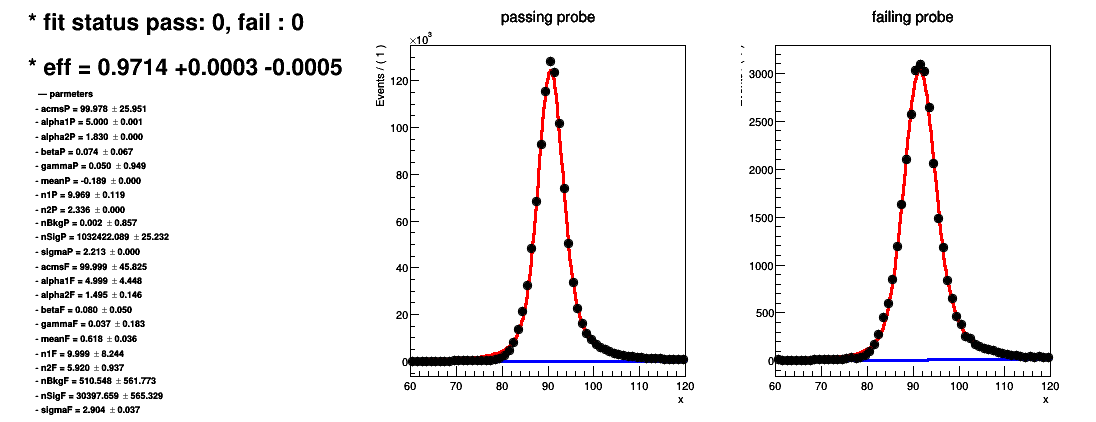
\includegraphics[height=0.355\textheight]{fits/woNF/unseed_EB_R9_0p55to0p85_et45.png}\\[2pt]
  {\scriptsize\hl{with NF}}\\[1pt]
  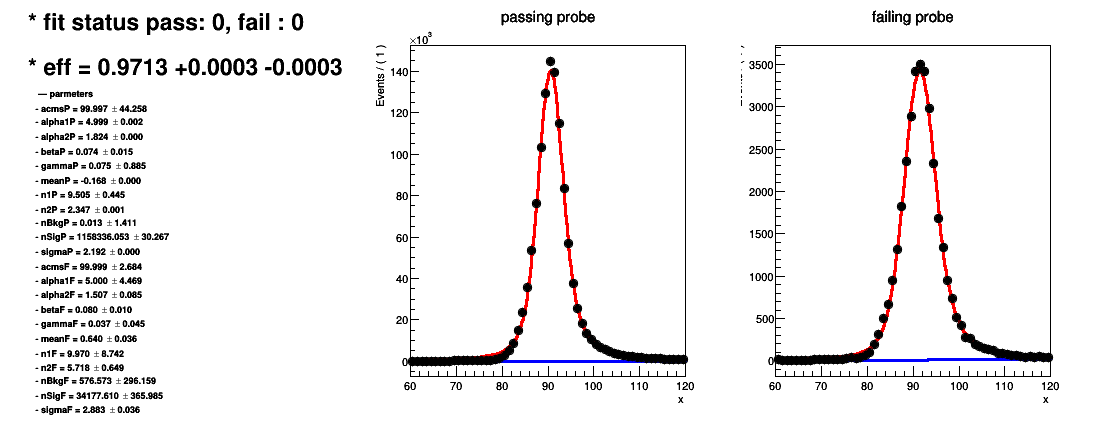
\includegraphics[height=0.355\textheight]{fits/wNF/unseed_EB_R9_0p55to0p85_et45.png}\\[2pt]
  \vspace{-10pt}\hfill\hyperlink{eff-unseed-EB}{\beamerreturnbutton{efficiency}}
\end{frame}

\begin{frame}[label=fit-unseed-EB-R9-0p55to0p85-50]{Fits: unseeded leg, EB $0.55<\RNine<0.85$, $50<\ET<60$~GeV}
  \centering
  {\scriptsize\hl{without NF}}\\[1pt]
  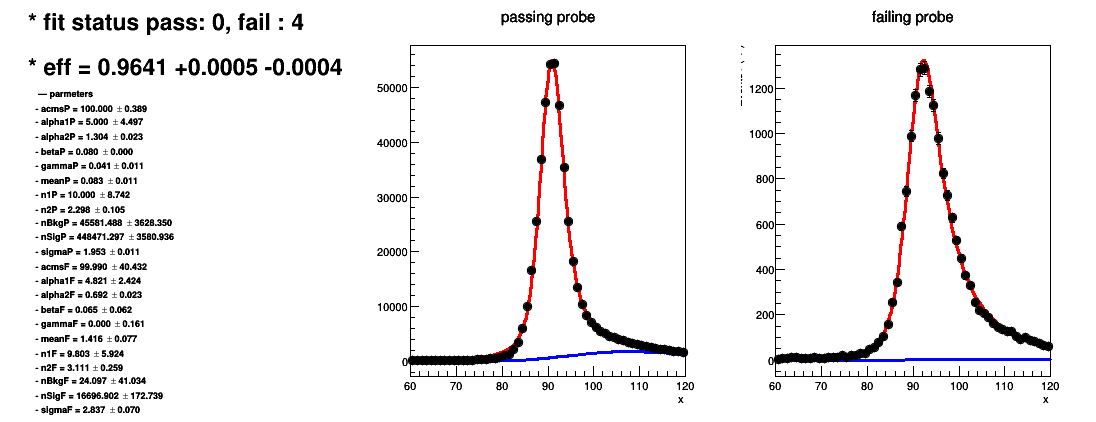
\includegraphics[height=0.355\textheight]{fits/woNF/unseed_EB_R9_0p55to0p85_et50.png}\\[2pt]
  {\scriptsize\hl{with NF}}\\[1pt]
  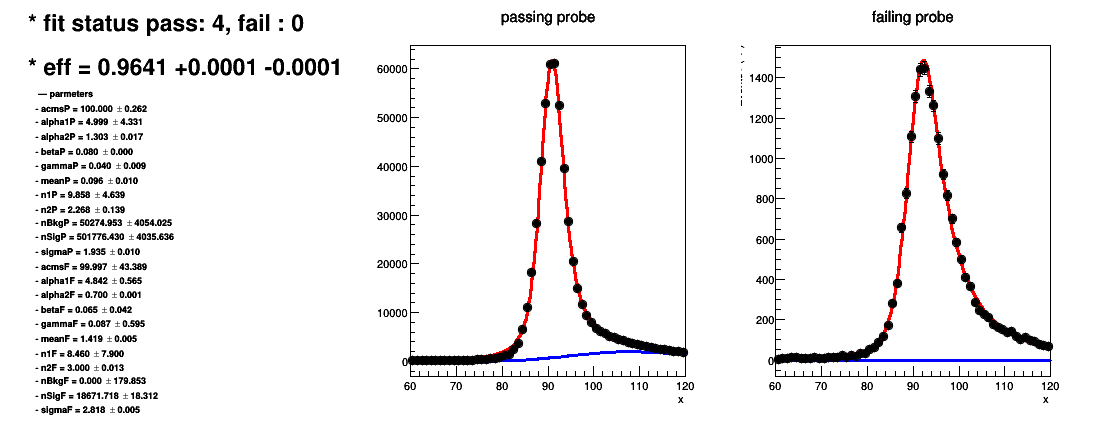
\includegraphics[height=0.355\textheight]{fits/wNF/unseed_EB_R9_0p55to0p85_et50.png}\\[2pt]
  \vspace{-10pt}\hfill\hyperlink{eff-unseed-EB}{\beamerreturnbutton{efficiency}}
\end{frame}

\begin{frame}[label=fit-unseed-EB-R9-0p55to0p85-60]{Fits: unseeded leg, EB $0.55<\RNine<0.85$, $60<\ET<70$~GeV}
  \centering
  {\scriptsize\hl{without NF}}\\[1pt]
  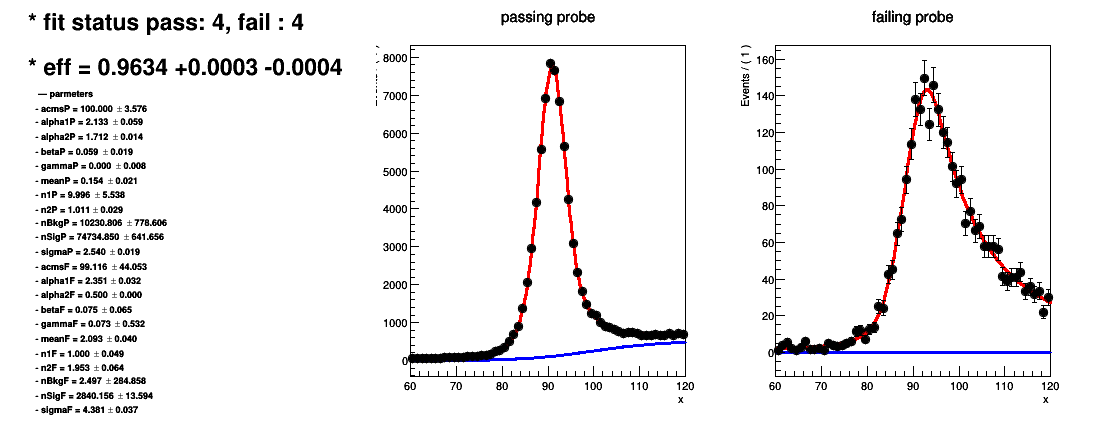
\includegraphics[height=0.355\textheight]{fits/woNF/unseed_EB_R9_0p55to0p85_et60.png}\\[2pt]
  {\scriptsize\hl{with NF}}\\[1pt]
  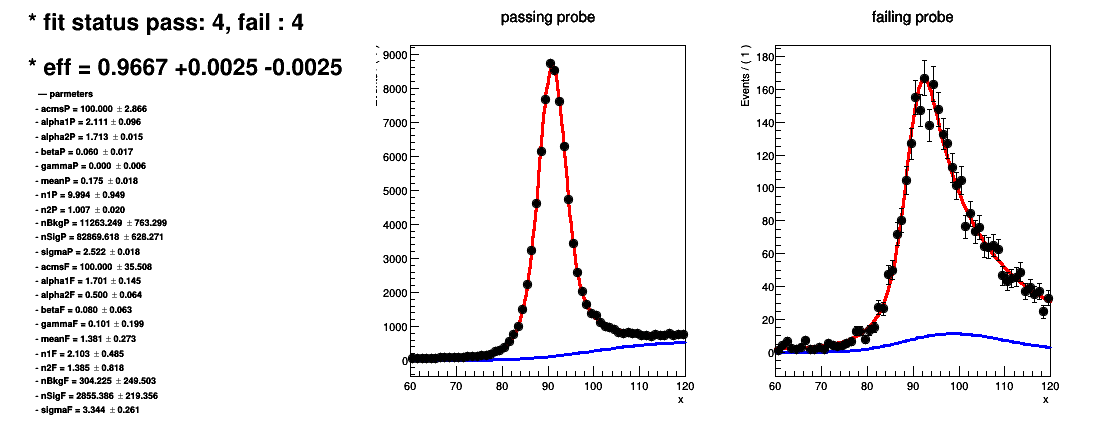
\includegraphics[height=0.355\textheight]{fits/wNF/unseed_EB_R9_0p55to0p85_et60.png}\\[2pt]
  \vspace{-10pt}\hfill\hyperlink{eff-unseed-EB}{\beamerreturnbutton{efficiency}}
\end{frame}

\begin{frame}[label=fit-unseed-EB-R9-0p55to0p85-70]{Fits: unseeded leg, EB $0.55<\RNine<0.85$, $70<\ET<90$~GeV}
  \centering
  {\scriptsize\hl{without NF}}\\[1pt]
  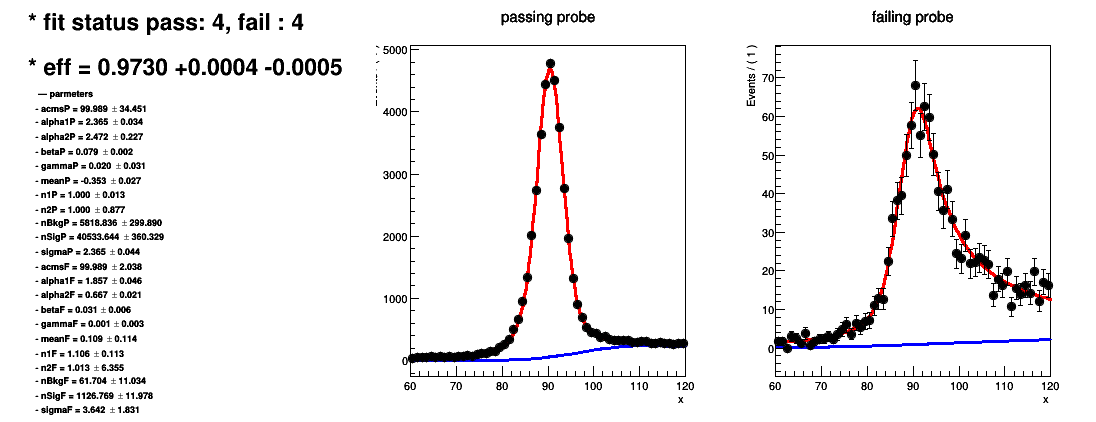
\includegraphics[height=0.355\textheight]{fits/woNF/unseed_EB_R9_0p55to0p85_et70.png}\\[2pt]
  {\scriptsize\hl{with NF}}\\[1pt]
  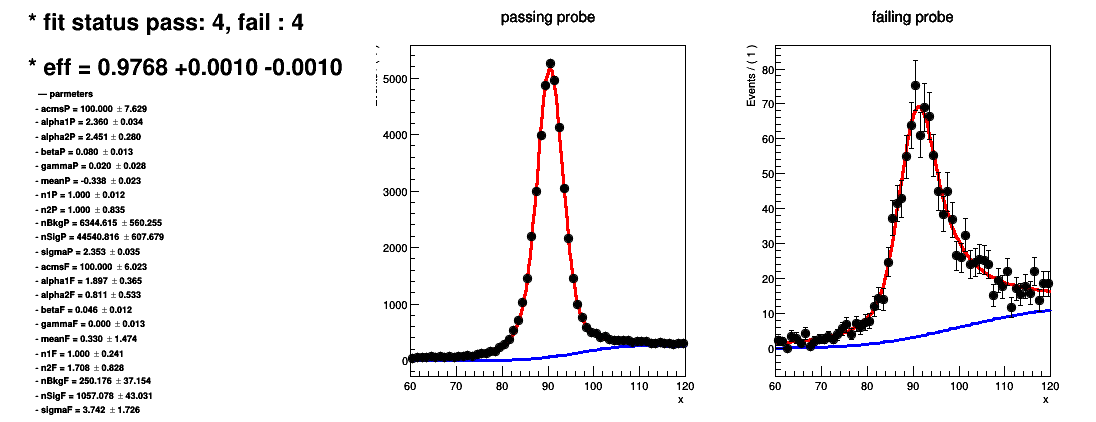
\includegraphics[height=0.355\textheight]{fits/wNF/unseed_EB_R9_0p55to0p85_et70.png}\\[2pt]
  \vspace{-10pt}\hfill\hyperlink{eff-unseed-EB}{\beamerreturnbutton{efficiency}}
\end{frame}

\begin{frame}[label=fit-unseed-EB-R9-0p55to0p85-90]{Fits: unseeded leg, EB $0.55<\RNine<0.85$, $\ET>90$~GeV}
  \centering
  {\scriptsize\hl{without NF}}\\[1pt]
  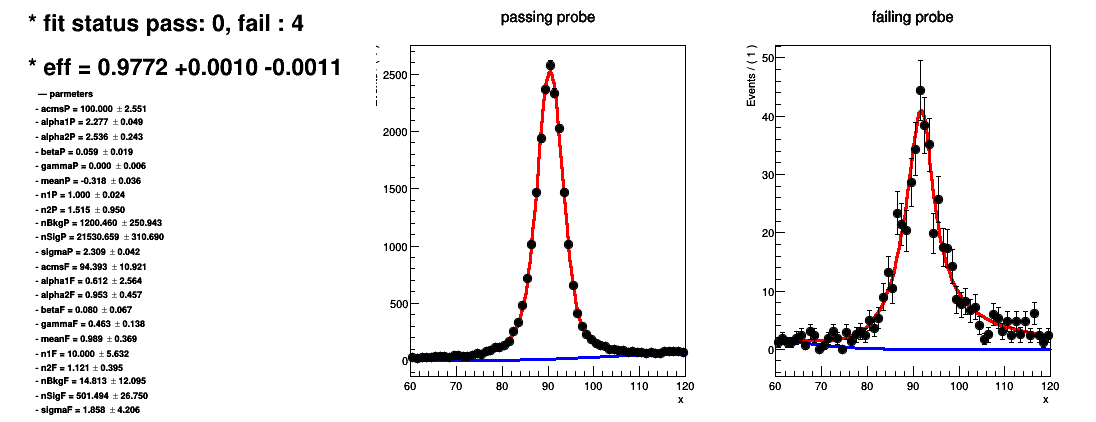
\includegraphics[height=0.355\textheight]{fits/woNF/unseed_EB_R9_0p55to0p85_et90.png}\\[2pt]
  {\scriptsize\hl{with NF}}\\[1pt]
  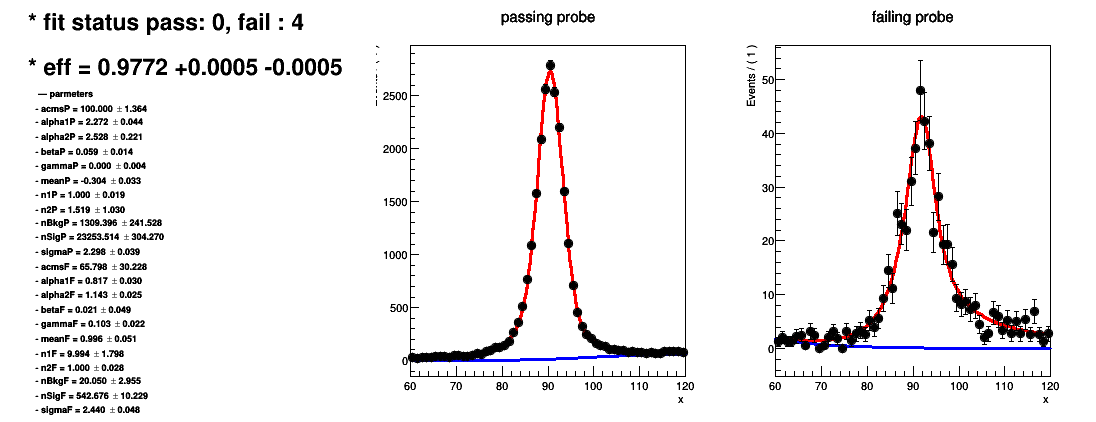
\includegraphics[height=0.355\textheight]{fits/wNF/unseed_EB_R9_0p55to0p85_et90.png}\\[2pt]
  \vspace{-10pt}\hfill\hyperlink{eff-unseed-EB}{\beamerreturnbutton{efficiency}}
\end{frame}

\begin{frame}[label=fit-unseed-EB-R9gt0p85-0]{Fits: unseeded leg, EB $\RNine>0.85$, $0<\ET<21$~GeV}
  \centering
  {\scriptsize\hl{without NF}}\\[1pt]
  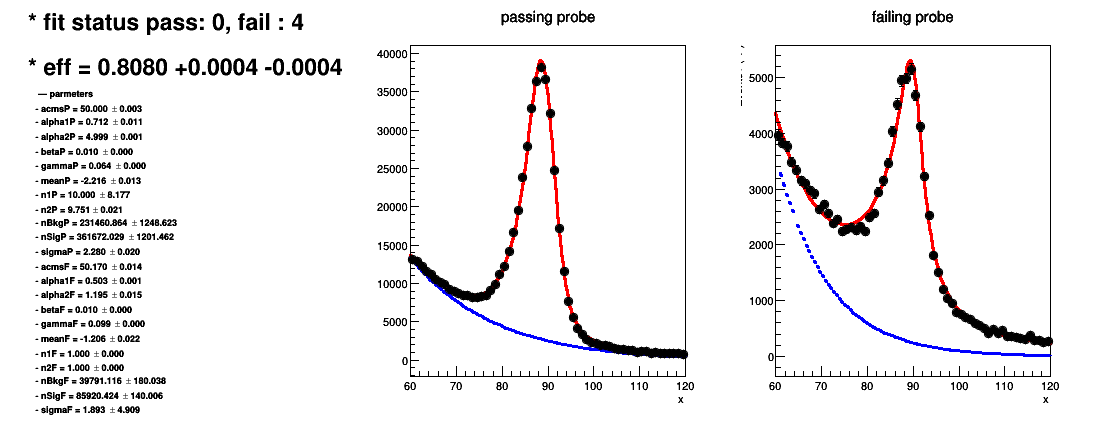
\includegraphics[height=0.355\textheight]{fits/woNF/unseed_EB_R9gt0p85_et0.png}\\[2pt]
  {\scriptsize\hl{with NF}}\\[1pt]
  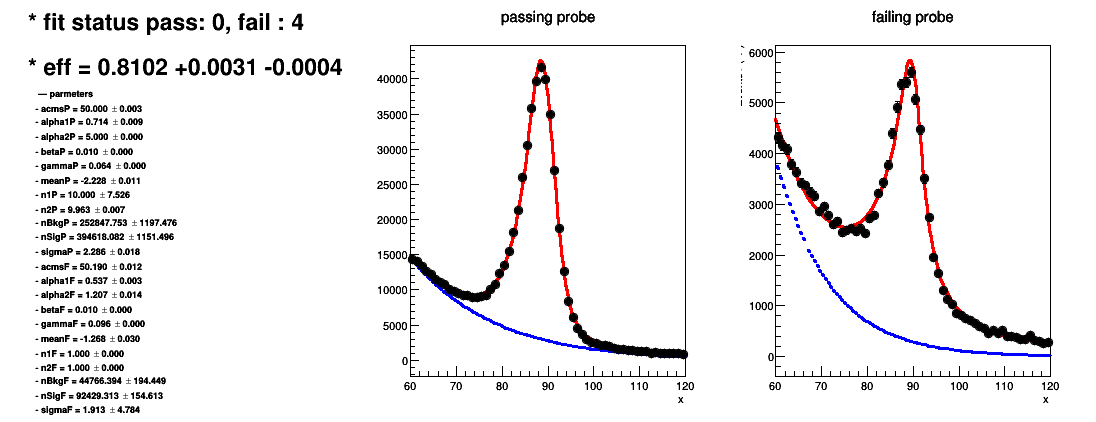
\includegraphics[height=0.355\textheight]{fits/wNF/unseed_EB_R9gt0p85_et0.png}\\[2pt]
  \vspace{-10pt}\hfill\hyperlink{eff-unseed-EB}{\beamerreturnbutton{efficiency}}
\end{frame}

\begin{frame}[label=fit-unseed-EB-R9gt0p85-21]{Fits: unseeded leg, EB $\RNine>0.85$, $21<\ET<25$~GeV}
  \centering
  {\scriptsize\hl{without NF}}\\[1pt]
  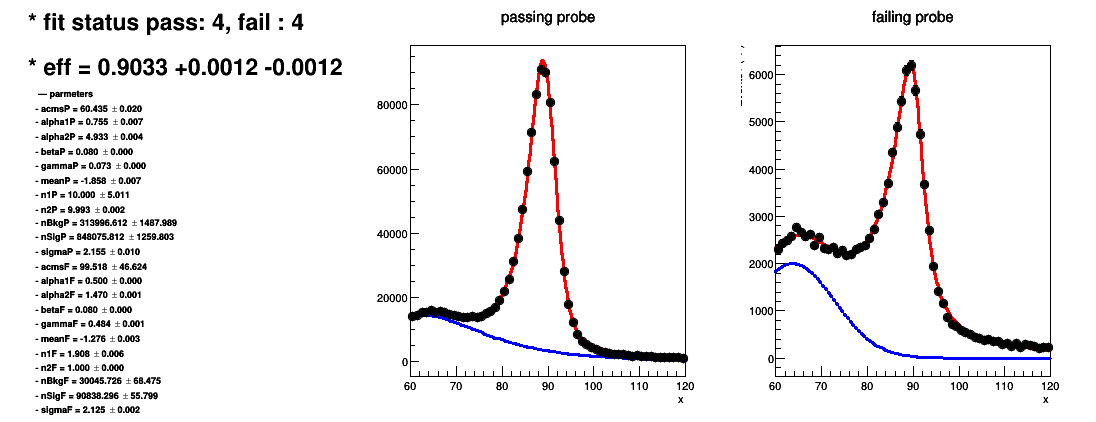
\includegraphics[height=0.355\textheight]{fits/woNF/unseed_EB_R9gt0p85_et21.png}\\[2pt]
  {\scriptsize\hl{with NF}}\\[1pt]
  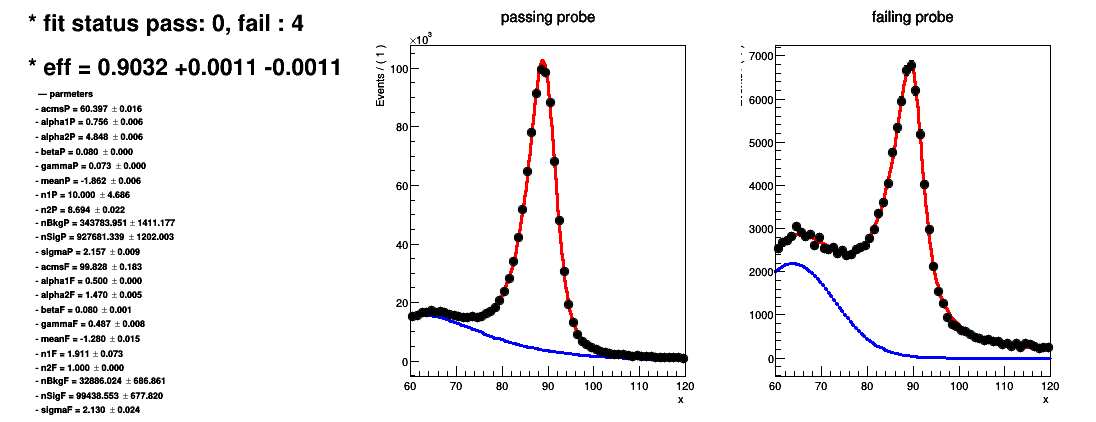
\includegraphics[height=0.355\textheight]{fits/wNF/unseed_EB_R9gt0p85_et21.png}\\[2pt]
  \vspace{-10pt}\hfill\hyperlink{eff-unseed-EB}{\beamerreturnbutton{efficiency}}
\end{frame}

\begin{frame}[label=fit-unseed-EB-R9gt0p85-25]{Fits: unseeded leg, EB $\RNine>0.85$, $25<\ET<28$~GeV}
  \centering
  {\scriptsize\hl{without NF}}\\[1pt]
  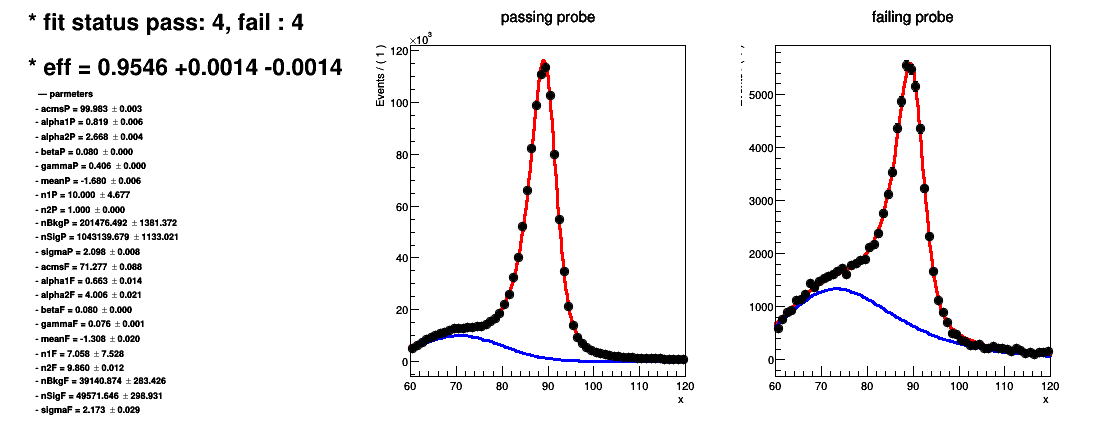
\includegraphics[height=0.355\textheight]{fits/woNF/unseed_EB_R9gt0p85_et25.png}\\[2pt]
  {\scriptsize\hl{with NF}}\\[1pt]
  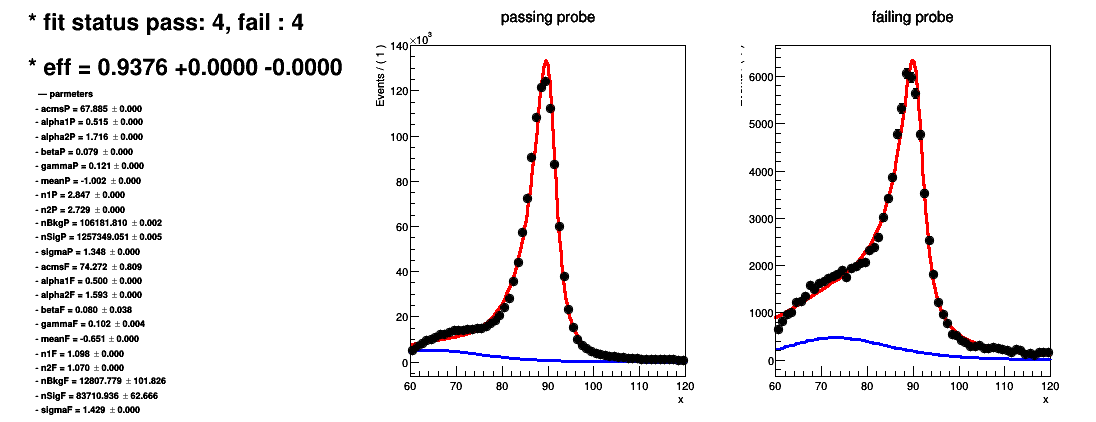
\includegraphics[height=0.355\textheight]{fits/wNF/unseed_EB_R9gt0p85_et25.png}\\[2pt]
  \vspace{-10pt}\hfill\hyperlink{eff-unseed-EB}{\beamerreturnbutton{efficiency}}
\end{frame}

\begin{frame}[label=fit-unseed-EB-R9gt0p85-28]{Fits: unseeded leg, EB $\RNine>0.85$, $28<\ET<31$~GeV}
  \centering
  {\scriptsize\hl{without NF}}\\[1pt]
  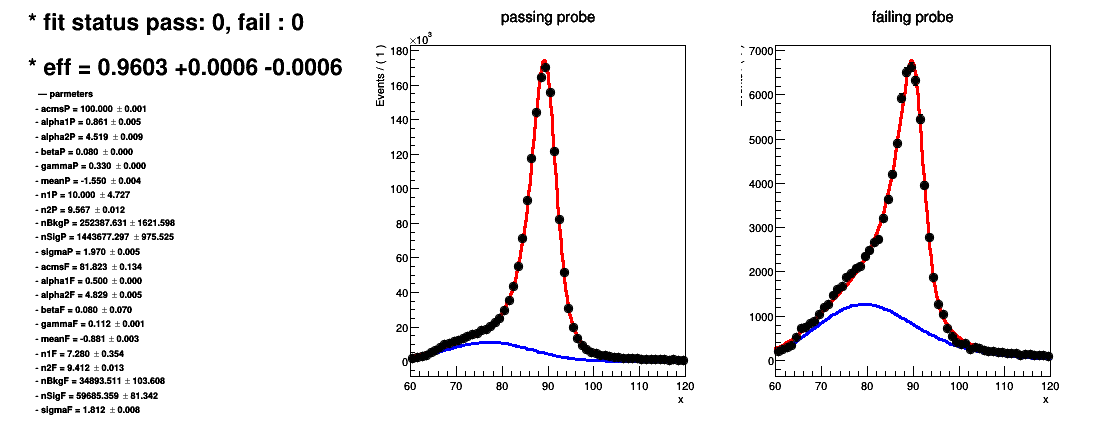
\includegraphics[height=0.355\textheight]{fits/woNF/unseed_EB_R9gt0p85_et28.png}\\[2pt]
  {\scriptsize\hl{with NF}}\\[1pt]
  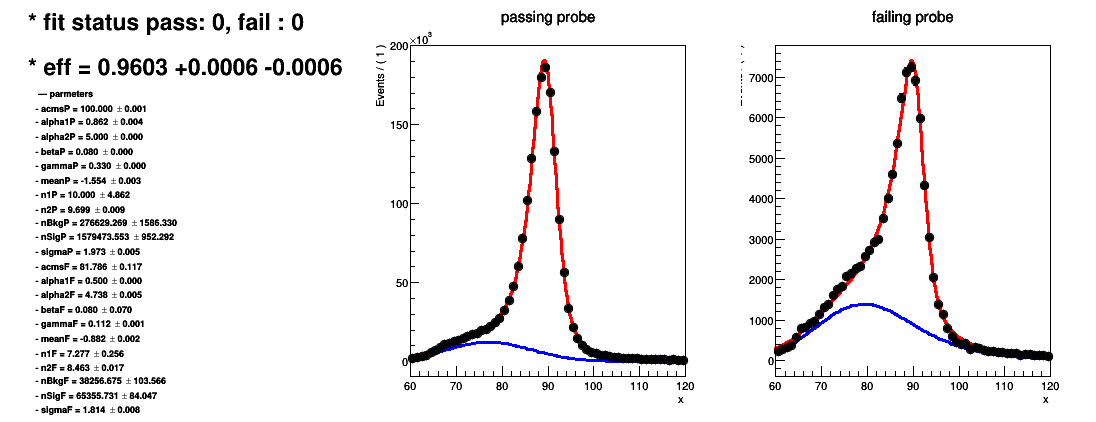
\includegraphics[height=0.355\textheight]{fits/wNF/unseed_EB_R9gt0p85_et28.png}\\[2pt]
  \vspace{-10pt}\hfill\hyperlink{eff-unseed-EB}{\beamerreturnbutton{efficiency}}
\end{frame}

\begin{frame}[label=fit-unseed-EB-R9gt0p85-31]{Fits: unseeded leg, EB $\RNine>0.85$, $31<\ET<35$~GeV}
  \centering
  {\scriptsize\hl{without NF}}\\[1pt]
  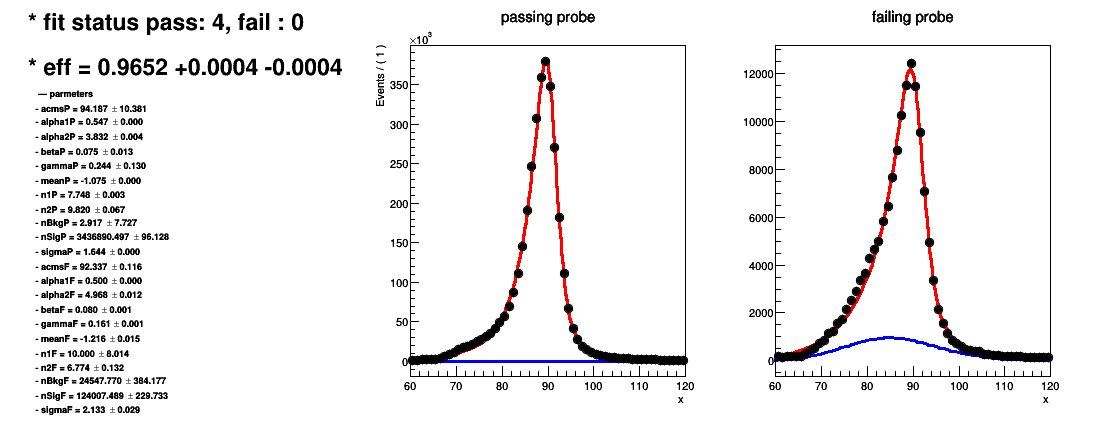
\includegraphics[height=0.355\textheight]{fits/woNF/unseed_EB_R9gt0p85_et31.png}\\[2pt]
  {\scriptsize\hl{with NF}}\\[1pt]
  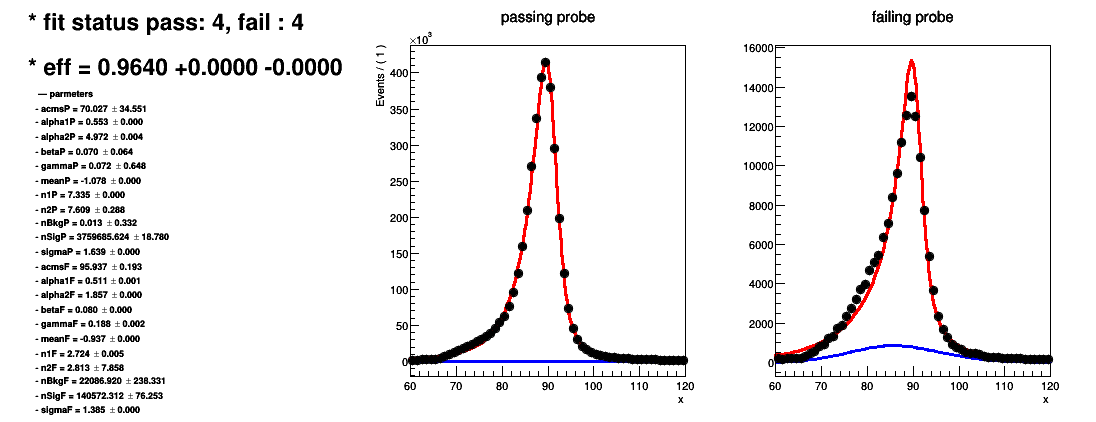
\includegraphics[height=0.355\textheight]{fits/wNF/unseed_EB_R9gt0p85_et31.png}\\[2pt]
  \vspace{-10pt}\hfill\hyperlink{eff-unseed-EB}{\beamerreturnbutton{efficiency}}
\end{frame}

\begin{frame}[label=fit-unseed-EB-R9gt0p85-35]{Fits: unseeded leg, EB $\RNine>0.85$, $35<\ET<40$~GeV}
  \centering
  {\scriptsize\hl{without NF}}\\[1pt]
  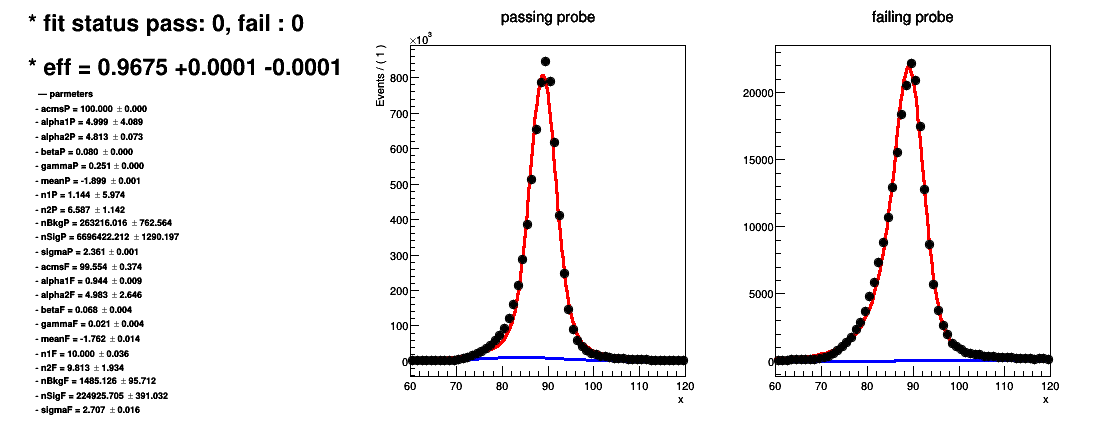
\includegraphics[height=0.355\textheight]{fits/woNF/unseed_EB_R9gt0p85_et35.png}\\[2pt]
  {\scriptsize\hl{with NF}}\\[1pt]
  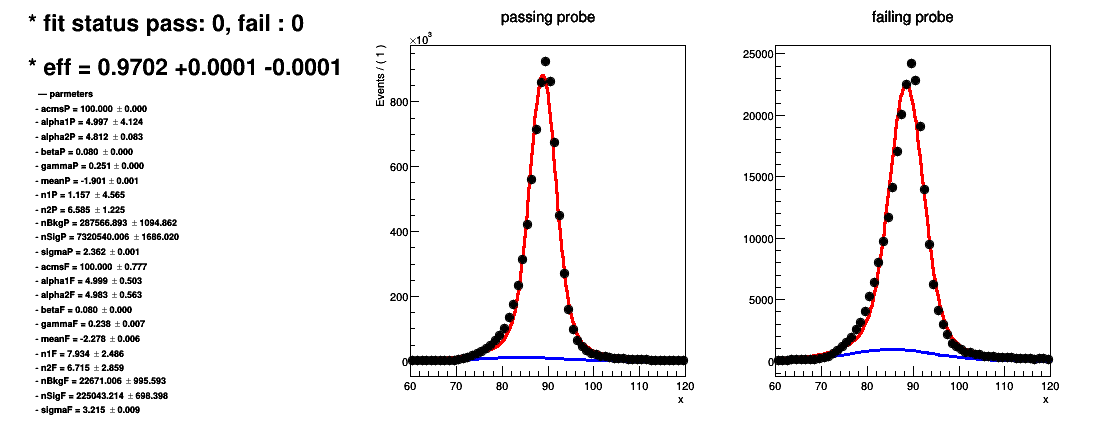
\includegraphics[height=0.355\textheight]{fits/wNF/unseed_EB_R9gt0p85_et35.png}\\[2pt]
  \vspace{-10pt}\hfill\hyperlink{eff-unseed-EB}{\beamerreturnbutton{efficiency}}
\end{frame}

\begin{frame}[label=fit-unseed-EB-R9gt0p85-40]{Fits: unseeded leg, EB $\RNine>0.85$, $40<\ET<45$~GeV}
  \centering
  {\scriptsize\hl{without NF}}\\[1pt]
  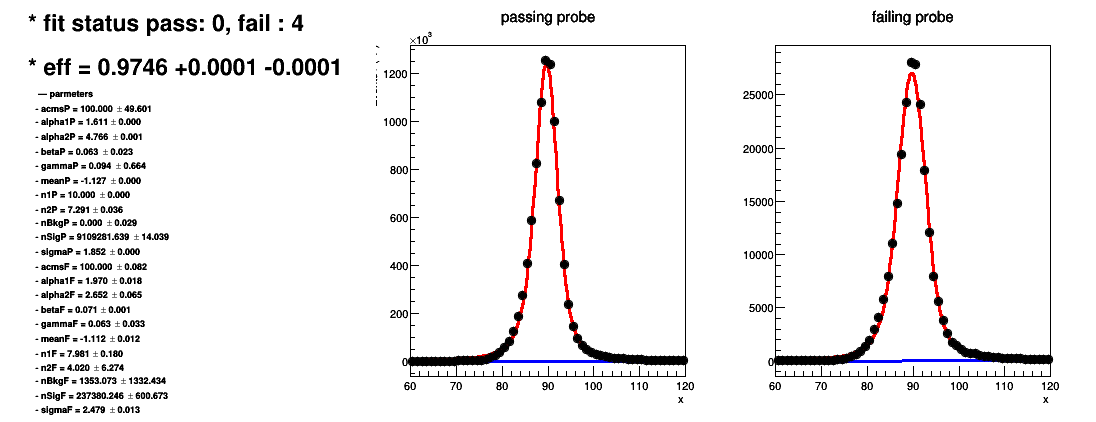
\includegraphics[height=0.355\textheight]{fits/woNF/unseed_EB_R9gt0p85_et40.png}\\[2pt]
  {\scriptsize\hl{with NF}}\\[1pt]
  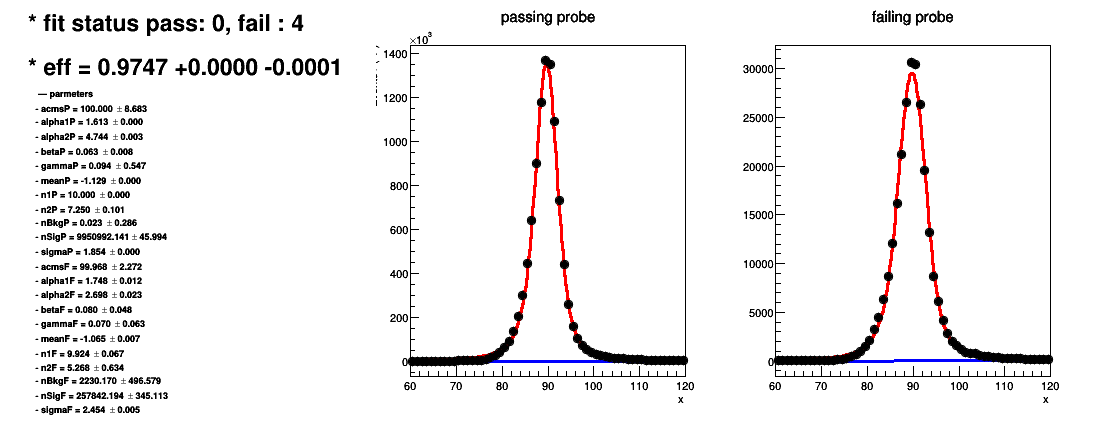
\includegraphics[height=0.355\textheight]{fits/wNF/unseed_EB_R9gt0p85_et40.png}\\[2pt]
  \vspace{-10pt}\hfill\hyperlink{eff-unseed-EB}{\beamerreturnbutton{efficiency}}
\end{frame}

\begin{frame}[label=fit-unseed-EB-R9gt0p85-45]{Fits: unseeded leg, EB $\RNine>0.85$, $45<\ET<50$~GeV}
  \centering
  {\scriptsize\hl{without NF}}\\[1pt]
  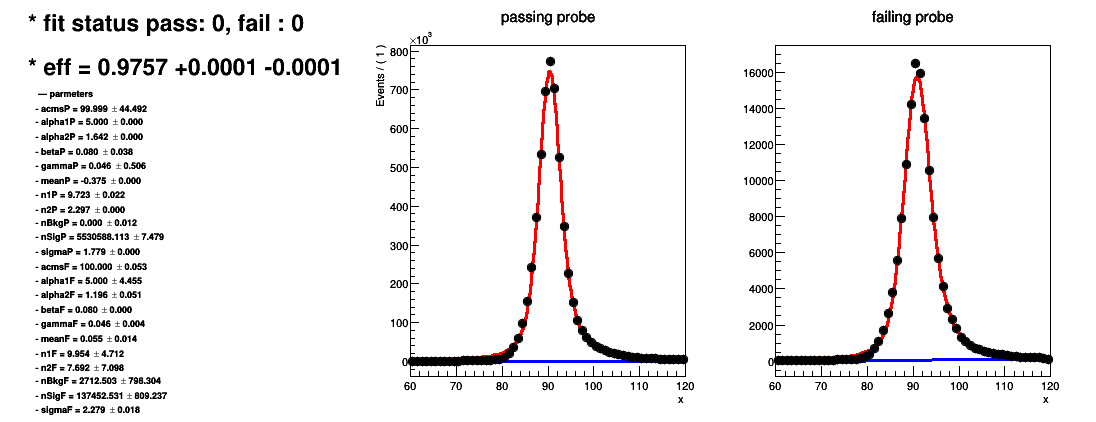
\includegraphics[height=0.355\textheight]{fits/woNF/unseed_EB_R9gt0p85_et45.png}\\[2pt]
  {\scriptsize\hl{with NF}}\\[1pt]
  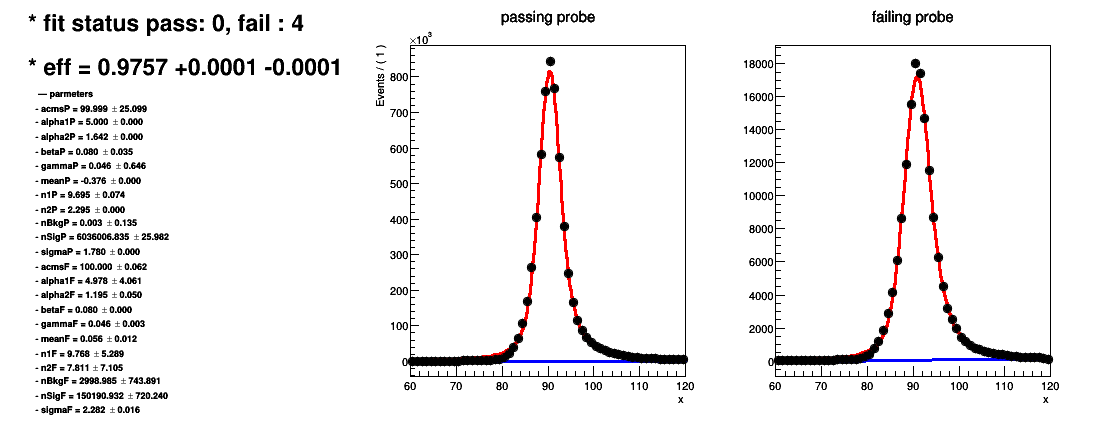
\includegraphics[height=0.355\textheight]{fits/wNF/unseed_EB_R9gt0p85_et45.png}\\[2pt]
  \vspace{-10pt}\hfill\hyperlink{eff-unseed-EB}{\beamerreturnbutton{efficiency}}
\end{frame}

\begin{frame}[label=fit-unseed-EB-R9gt0p85-50]{Fits: unseeded leg, EB $\RNine>0.85$, $50<\ET<60$~GeV}
  \centering
  {\scriptsize\hl{without NF}}\\[1pt]
  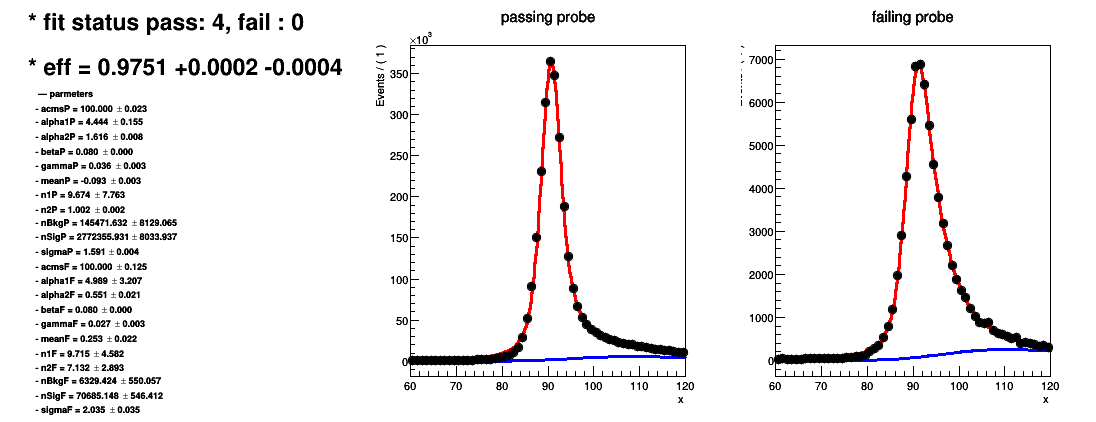
\includegraphics[height=0.355\textheight]{fits/woNF/unseed_EB_R9gt0p85_et50.png}\\[2pt]
  {\scriptsize\hl{with NF}}\\[1pt]
  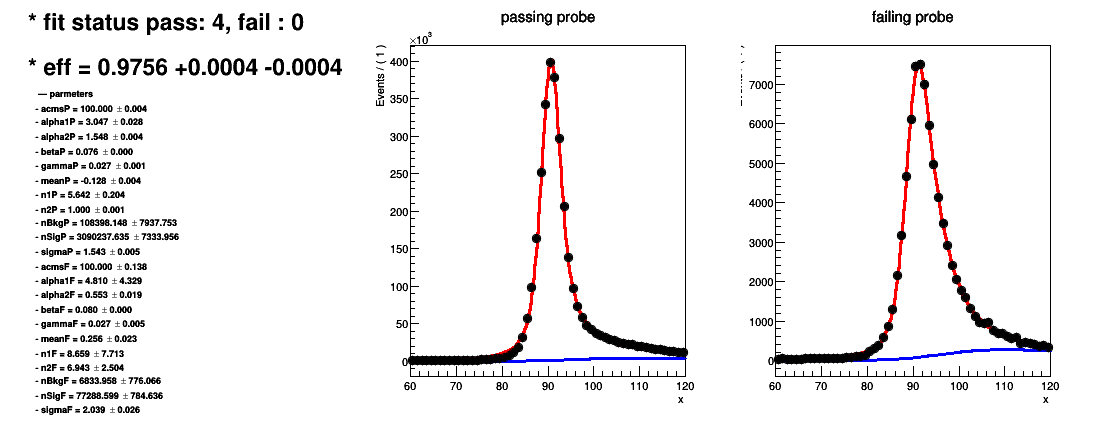
\includegraphics[height=0.355\textheight]{fits/wNF/unseed_EB_R9gt0p85_et50.png}\\[2pt]
  \vspace{-10pt}\hfill\hyperlink{eff-unseed-EB}{\beamerreturnbutton{efficiency}}
\end{frame}

\begin{frame}[label=fit-unseed-EB-R9gt0p85-60]{Fits: unseeded leg, EB $\RNine>0.85$, $60<\ET<70$~GeV}
  \centering
  {\scriptsize\hl{without NF}}\\[1pt]
  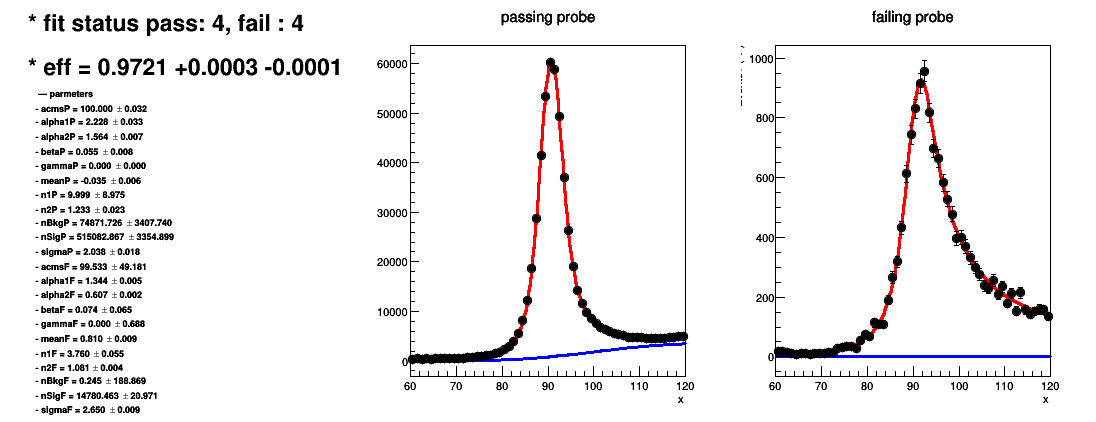
\includegraphics[height=0.355\textheight]{fits/woNF/unseed_EB_R9gt0p85_et60.png}\\[2pt]
  {\scriptsize\hl{with NF}}\\[1pt]
  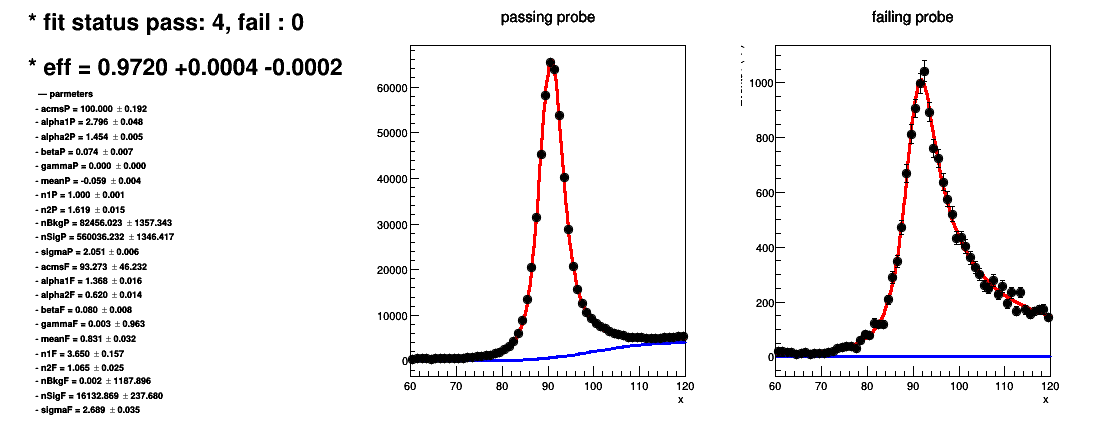
\includegraphics[height=0.355\textheight]{fits/wNF/unseed_EB_R9gt0p85_et60.png}\\[2pt]
  \vspace{-10pt}\hfill\hyperlink{eff-unseed-EB}{\beamerreturnbutton{efficiency}}
\end{frame}

\begin{frame}[label=fit-unseed-EB-R9gt0p85-70]{Fits: unseeded leg, EB $\RNine>0.85$, $70<\ET<90$~GeV}
  \centering
  {\scriptsize\hl{without NF}}\\[1pt]
  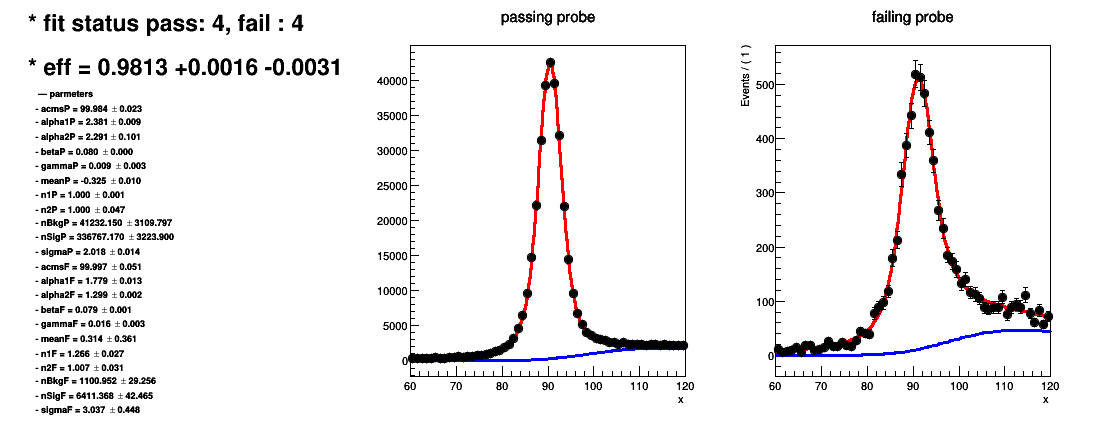
\includegraphics[height=0.355\textheight]{fits/woNF/unseed_EB_R9gt0p85_et70.png}\\[2pt]
  {\scriptsize\hl{with NF}}\\[1pt]
  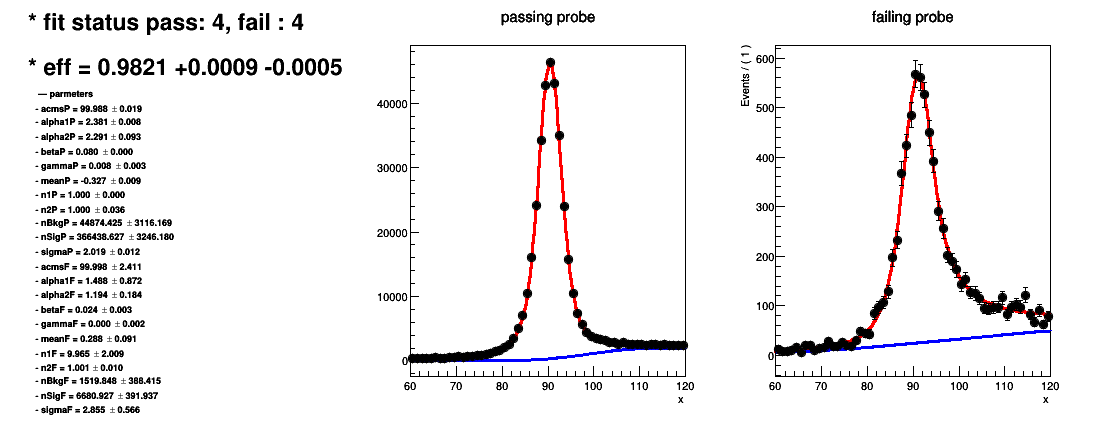
\includegraphics[height=0.355\textheight]{fits/wNF/unseed_EB_R9gt0p85_et70.png}\\[2pt]
  \vspace{-10pt}\hfill\hyperlink{eff-unseed-EB}{\beamerreturnbutton{efficiency}}
\end{frame}

\begin{frame}[label=fit-unseed-EB-R9gt0p85-90]{Fits: unseeded leg, EB $\RNine>0.85$, $\ET>90$~GeV}
  \centering
  {\scriptsize\hl{without NF}}\\[1pt]
  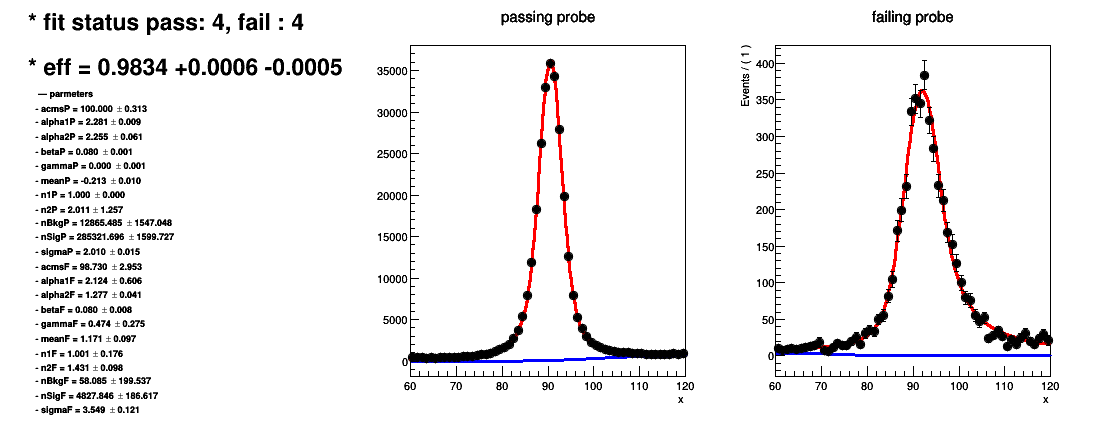
\includegraphics[height=0.355\textheight]{fits/woNF/unseed_EB_R9gt0p85_et90.png}\\[2pt]
  {\scriptsize\hl{with NF}}\\[1pt]
  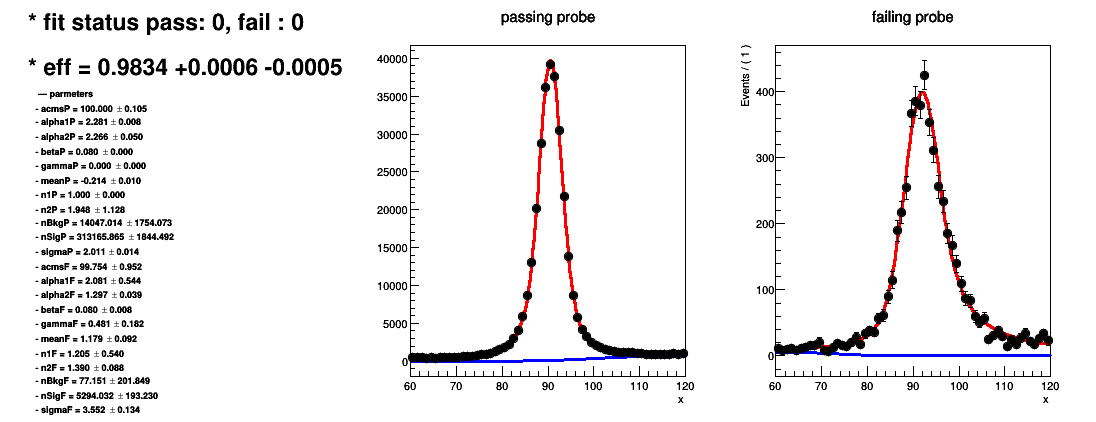
\includegraphics[height=0.355\textheight]{fits/wNF/unseed_EB_R9gt0p85_et90.png}\\[2pt]
  \vspace{-10pt}\hfill\hyperlink{eff-unseed-EB}{\beamerreturnbutton{efficiency}}
\end{frame}

\begin{frame}[label=fit-unseed-EE-R9-0p90to0p93-0]{Fits: unseeded leg, EE $0.90<\RNine<0.93$, $0<\ET<21$~GeV}
  \centering
  {\scriptsize\hl{without NF}}\\[1pt]
  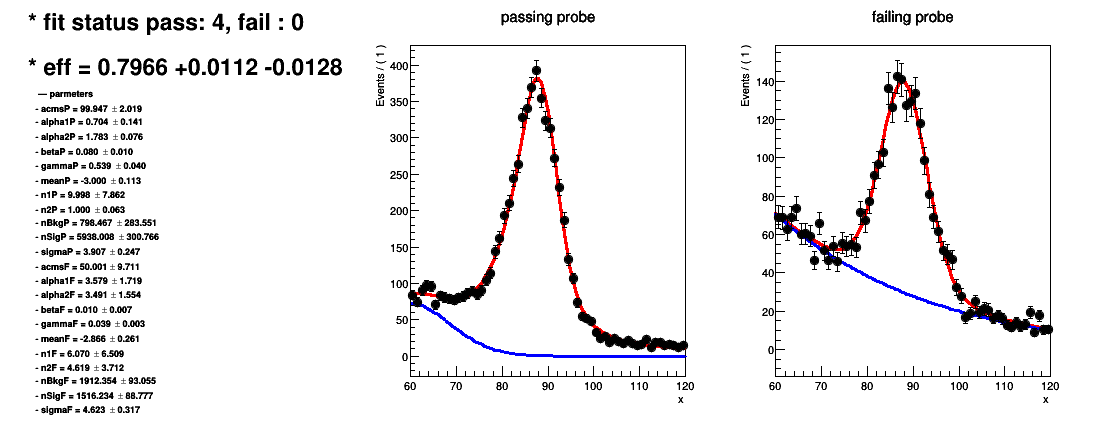
\includegraphics[height=0.355\textheight]{fits/woNF/unseed_EE_R9_0p90to0p93_et0.png}\\[2pt]
  {\scriptsize\hl{with NF}}\\[1pt]
  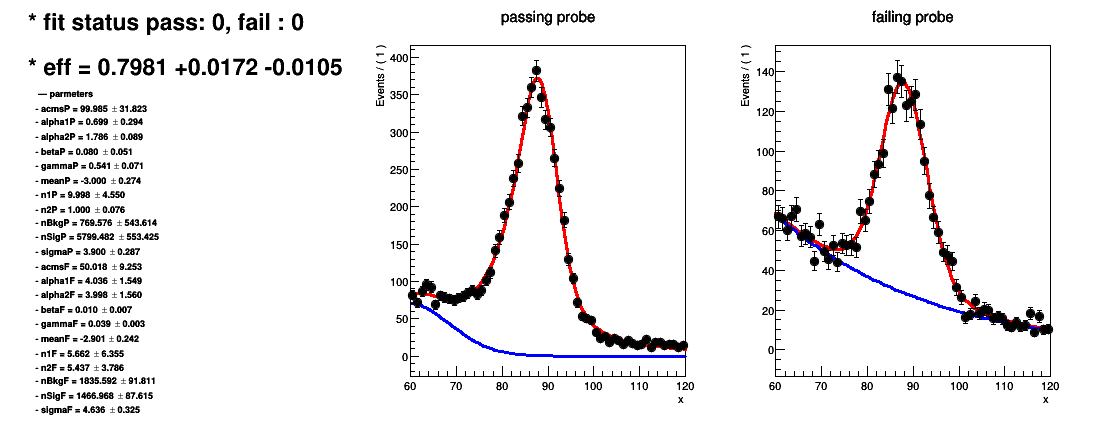
\includegraphics[height=0.355\textheight]{fits/wNF/unseed_EE_R9_0p90to0p93_et0.png}\\[2pt]
  \vspace{-10pt}\hfill\hyperlink{eff-unseed-EE}{\beamerreturnbutton{efficiency}}
\end{frame}

\begin{frame}[label=fit-unseed-EE-R9-0p90to0p93-21]{Fits: unseeded leg, EE $0.90<\RNine<0.93$, $21<\ET<25$~GeV}
  \centering
  {\scriptsize\hl{without NF}}\\[1pt]
  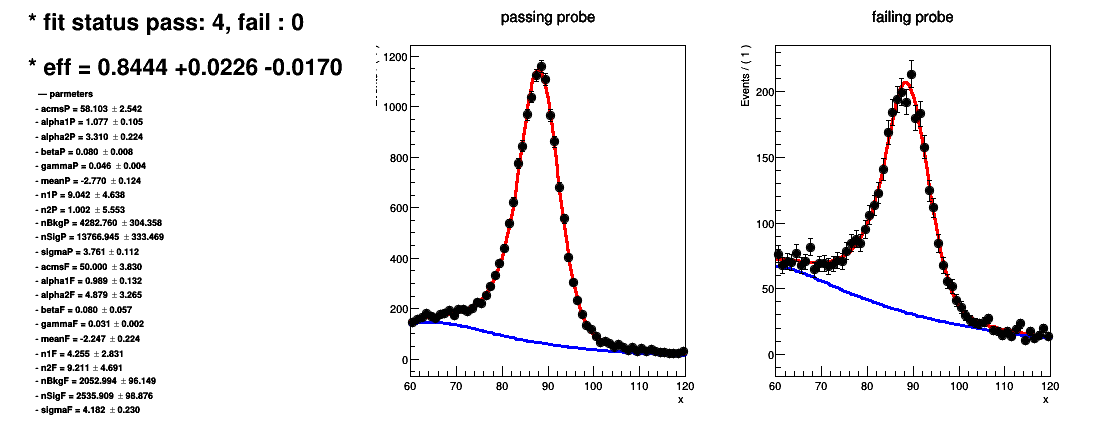
\includegraphics[height=0.355\textheight]{fits/woNF/unseed_EE_R9_0p90to0p93_et21.png}\\[2pt]
  {\scriptsize\hl{with NF}}\\[1pt]
  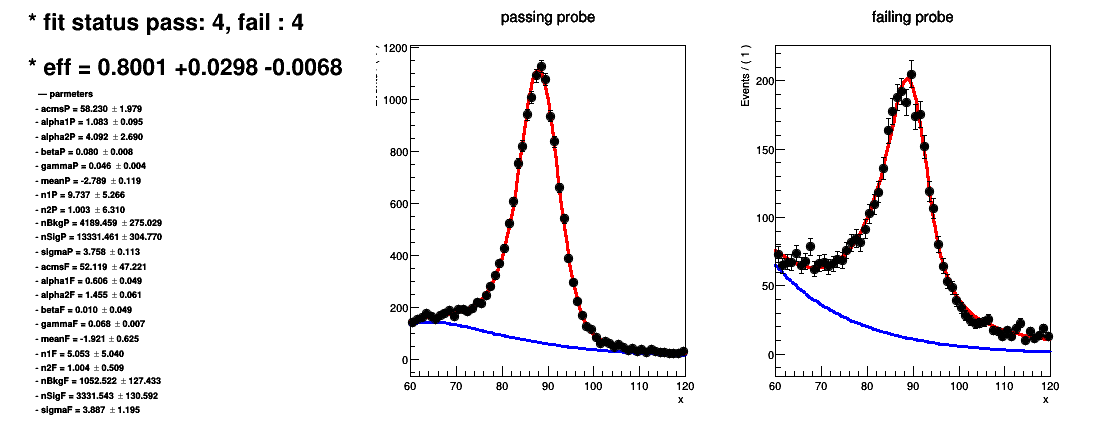
\includegraphics[height=0.355\textheight]{fits/wNF/unseed_EE_R9_0p90to0p93_et21.png}\\[2pt]
  \vspace{-10pt}\hfill\hyperlink{eff-unseed-EE}{\beamerreturnbutton{efficiency}}
\end{frame}

\begin{frame}[label=fit-unseed-EE-R9-0p90to0p93-25]{Fits: unseeded leg, EE $0.90<\RNine<0.93$, $25<\ET<28$~GeV}
  \centering
  {\scriptsize\hl{without NF}}\\[1pt]
  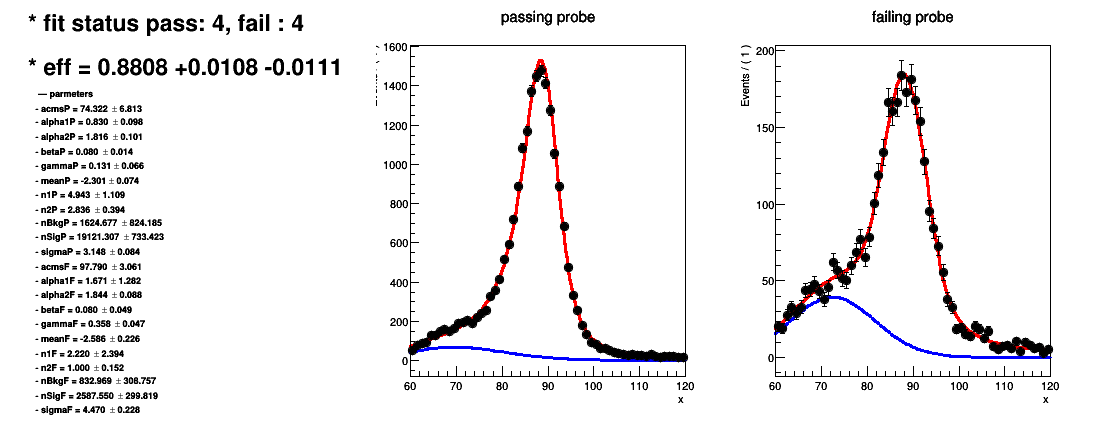
\includegraphics[height=0.355\textheight]{fits/woNF/unseed_EE_R9_0p90to0p93_et25.png}\\[2pt]
  {\scriptsize\hl{with NF}}\\[1pt]
  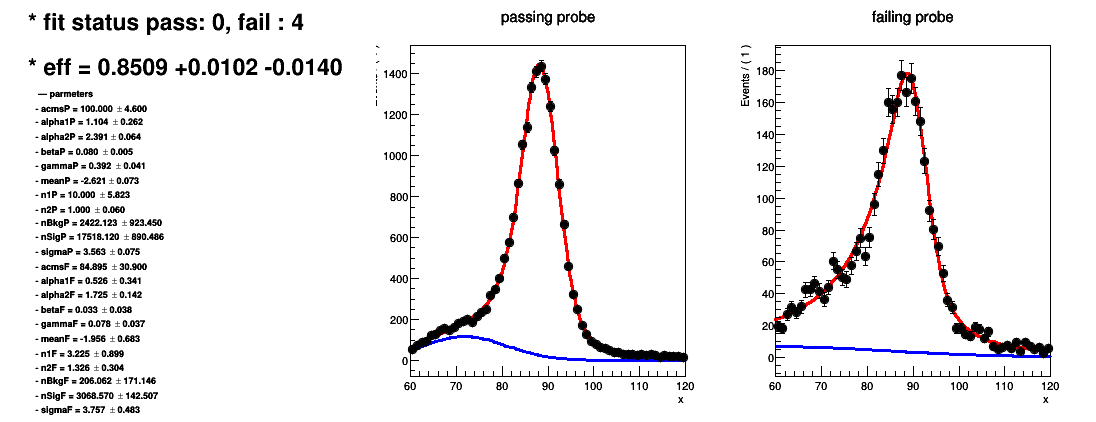
\includegraphics[height=0.355\textheight]{fits/wNF/unseed_EE_R9_0p90to0p93_et25.png}\\[2pt]
  \vspace{-10pt}\hfill\hyperlink{eff-unseed-EE}{\beamerreturnbutton{efficiency}}
\end{frame}

\begin{frame}[label=fit-unseed-EE-R9-0p90to0p93-28]{Fits: unseeded leg, EE $0.90<\RNine<0.93$, $28<\ET<31$~GeV}
  \centering
  {\scriptsize\hl{without NF}}\\[1pt]
  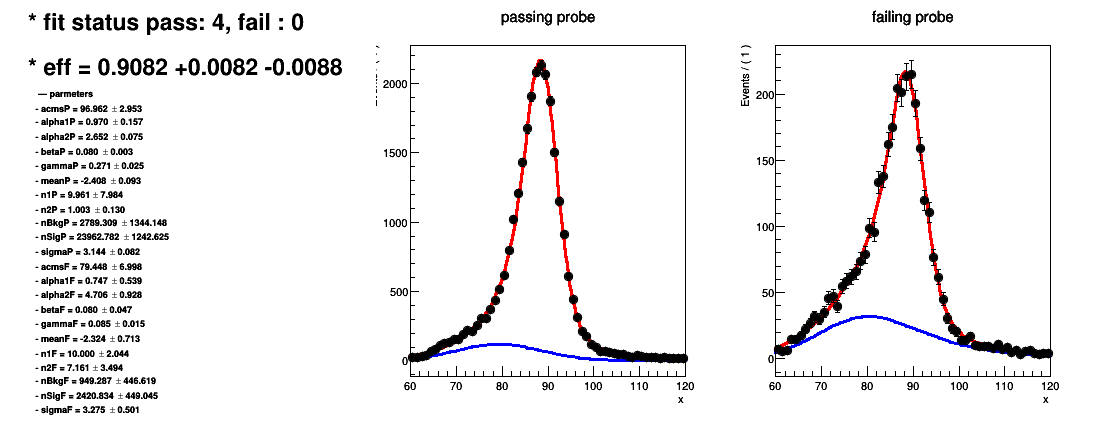
\includegraphics[height=0.355\textheight]{fits/woNF/unseed_EE_R9_0p90to0p93_et28.png}\\[2pt]
  {\scriptsize\hl{with NF}}\\[1pt]
  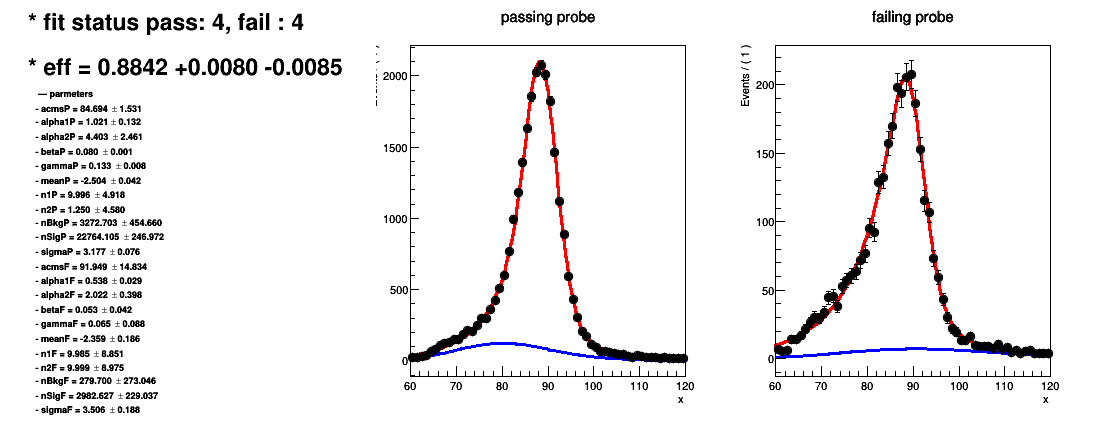
\includegraphics[height=0.355\textheight]{fits/wNF/unseed_EE_R9_0p90to0p93_et28.png}\\[2pt]
  \vspace{-10pt}\hfill\hyperlink{eff-unseed-EE}{\beamerreturnbutton{efficiency}}
\end{frame}

\begin{frame}[label=fit-unseed-EE-R9-0p90to0p93-31]{Fits: unseeded leg, EE $0.90<\RNine<0.93$, $31<\ET<35$~GeV}
  \centering
  {\scriptsize\hl{without NF}}\\[1pt]
  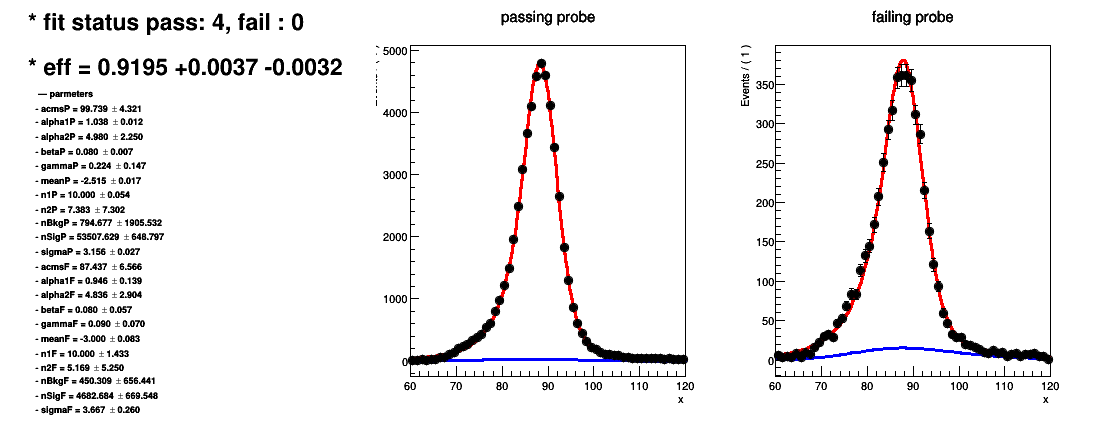
\includegraphics[height=0.355\textheight]{fits/woNF/unseed_EE_R9_0p90to0p93_et31.png}\\[2pt]
  {\scriptsize\hl{with NF}}\\[1pt]
  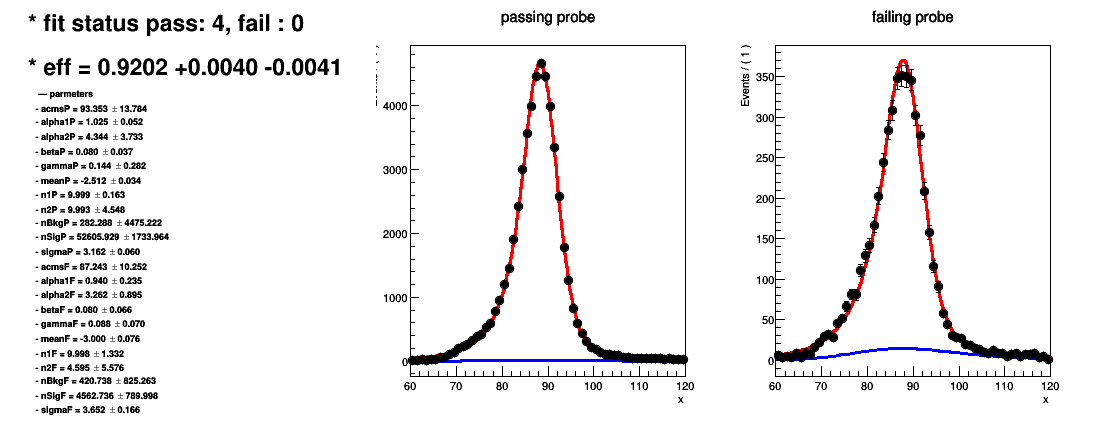
\includegraphics[height=0.355\textheight]{fits/wNF/unseed_EE_R9_0p90to0p93_et31.png}\\[2pt]
  \vspace{-10pt}\hfill\hyperlink{eff-unseed-EE}{\beamerreturnbutton{efficiency}}
\end{frame}

\begin{frame}[label=fit-unseed-EE-R9-0p90to0p93-35]{Fits: unseeded leg, EE $0.90<\RNine<0.93$, $35<\ET<40$~GeV}
  \centering
  {\scriptsize\hl{without NF}}\\[1pt]
  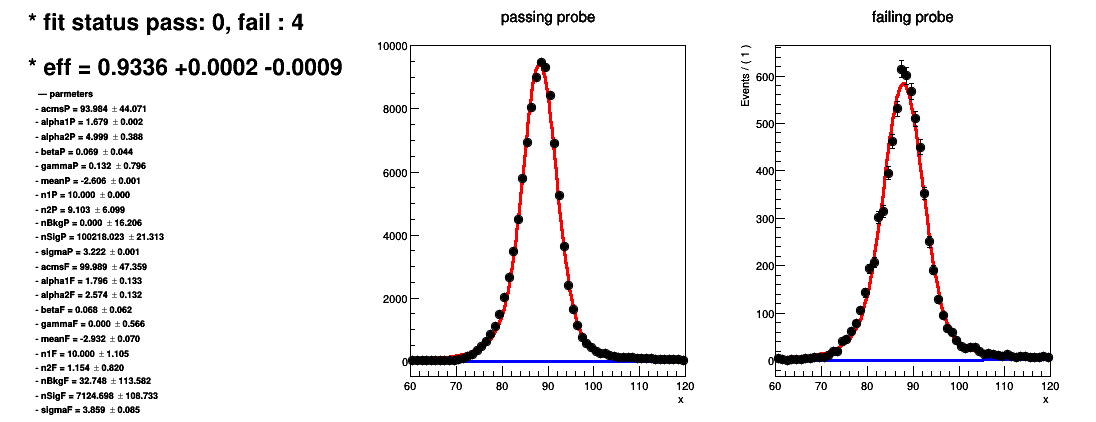
\includegraphics[height=0.355\textheight]{fits/woNF/unseed_EE_R9_0p90to0p93_et35.png}\\[2pt]
  {\scriptsize\hl{with NF}}\\[1pt]
  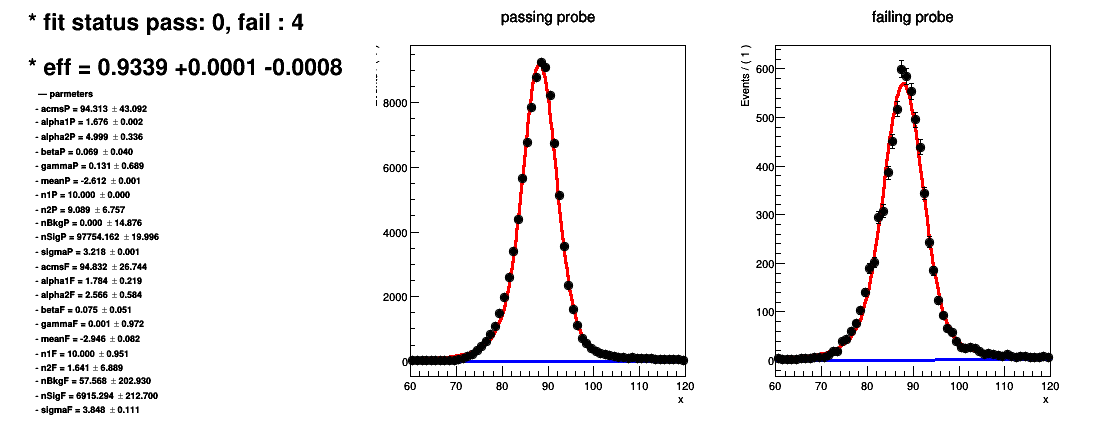
\includegraphics[height=0.355\textheight]{fits/wNF/unseed_EE_R9_0p90to0p93_et35.png}\\[2pt]
  \vspace{-10pt}\hfill\hyperlink{eff-unseed-EE}{\beamerreturnbutton{efficiency}}
\end{frame}

\begin{frame}[label=fit-unseed-EE-R9-0p90to0p93-40]{Fits: unseeded leg, EE $0.90<\RNine<0.93$, $40<\ET<45$~GeV}
  \centering
  {\scriptsize\hl{without NF}}\\[1pt]
  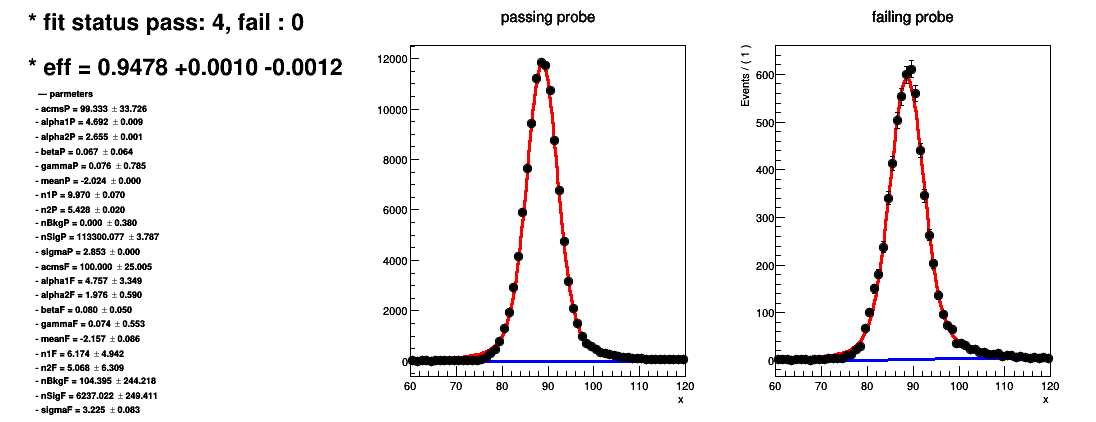
\includegraphics[height=0.355\textheight]{fits/woNF/unseed_EE_R9_0p90to0p93_et40.png}\\[2pt]
  {\scriptsize\hl{with NF}}\\[1pt]
  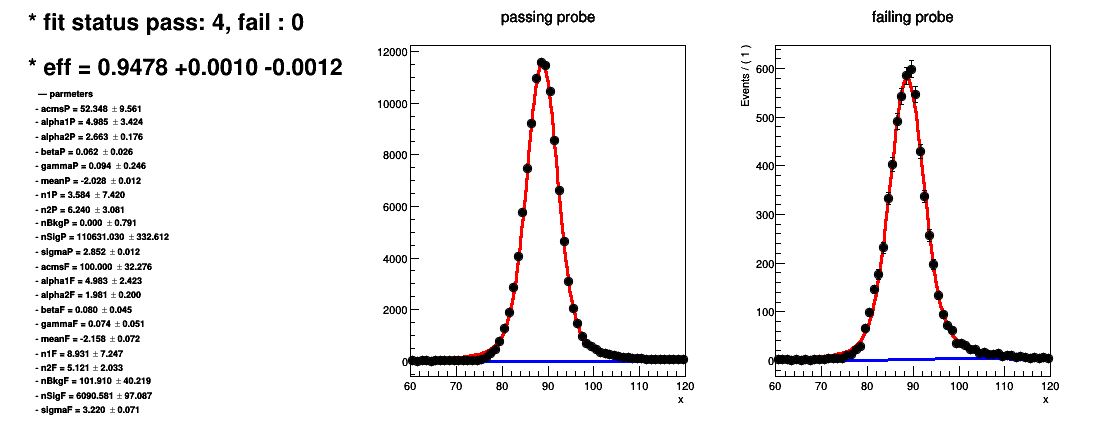
\includegraphics[height=0.355\textheight]{fits/wNF/unseed_EE_R9_0p90to0p93_et40.png}\\[2pt]
  \vspace{-10pt}\hfill\hyperlink{eff-unseed-EE}{\beamerreturnbutton{efficiency}}
\end{frame}

\begin{frame}[label=fit-unseed-EE-R9-0p90to0p93-45]{Fits: unseeded leg, EE $0.90<\RNine<0.93$, $45<\ET<50$~GeV}
  \centering
  {\scriptsize\hl{without NF}}\\[1pt]
  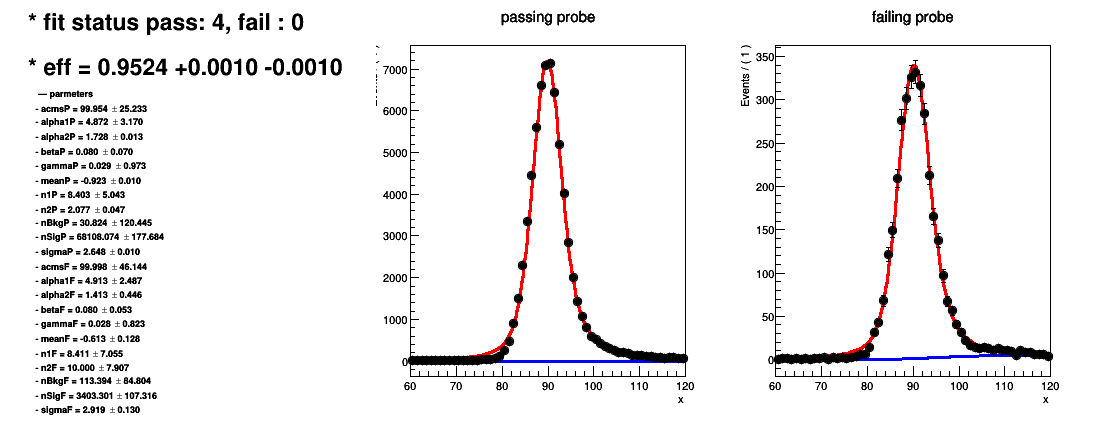
\includegraphics[height=0.355\textheight]{fits/woNF/unseed_EE_R9_0p90to0p93_et45.png}\\[2pt]
  {\scriptsize\hl{with NF}}\\[1pt]
  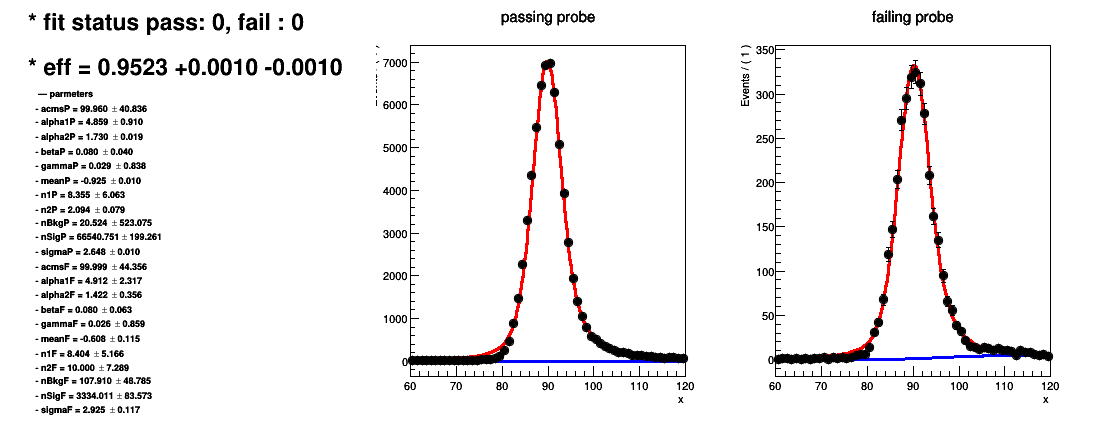
\includegraphics[height=0.355\textheight]{fits/wNF/unseed_EE_R9_0p90to0p93_et45.png}\\[2pt]
  \vspace{-10pt}\hfill\hyperlink{eff-unseed-EE}{\beamerreturnbutton{efficiency}}
\end{frame}

\begin{frame}[label=fit-unseed-EE-R9-0p90to0p93-50]{Fits: unseeded leg, EE $0.90<\RNine<0.93$, $50<\ET<60$~GeV}
  \centering
  {\scriptsize\hl{without NF}}\\[1pt]
  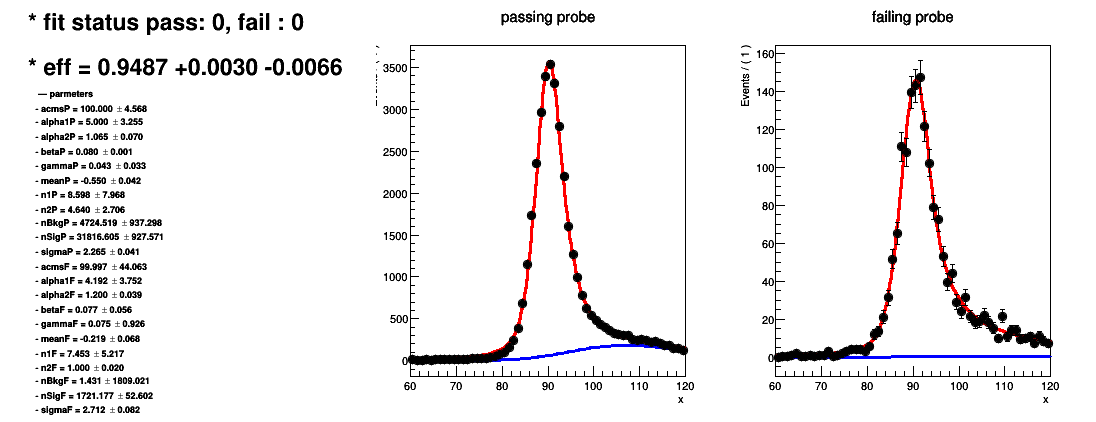
\includegraphics[height=0.355\textheight]{fits/woNF/unseed_EE_R9_0p90to0p93_et50.png}\\[2pt]
  {\scriptsize\hl{with NF}}\\[1pt]
  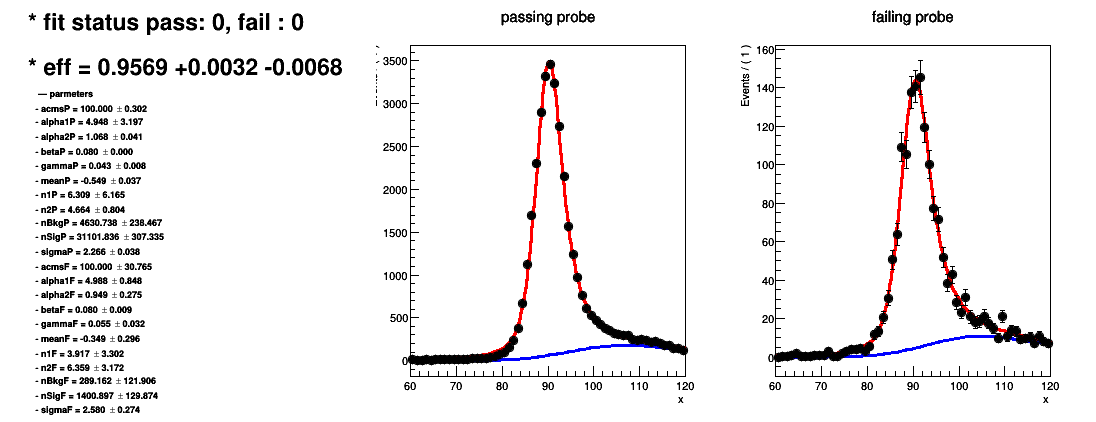
\includegraphics[height=0.355\textheight]{fits/wNF/unseed_EE_R9_0p90to0p93_et50.png}\\[2pt]
  \vspace{-10pt}\hfill\hyperlink{eff-unseed-EE}{\beamerreturnbutton{efficiency}}
\end{frame}

\begin{frame}[label=fit-unseed-EE-R9-0p90to0p93-60]{Fits: unseeded leg, EE $0.90<\RNine<0.93$, $60<\ET<70$~GeV}
  \centering
  {\scriptsize\hl{without NF}}\\[1pt]
  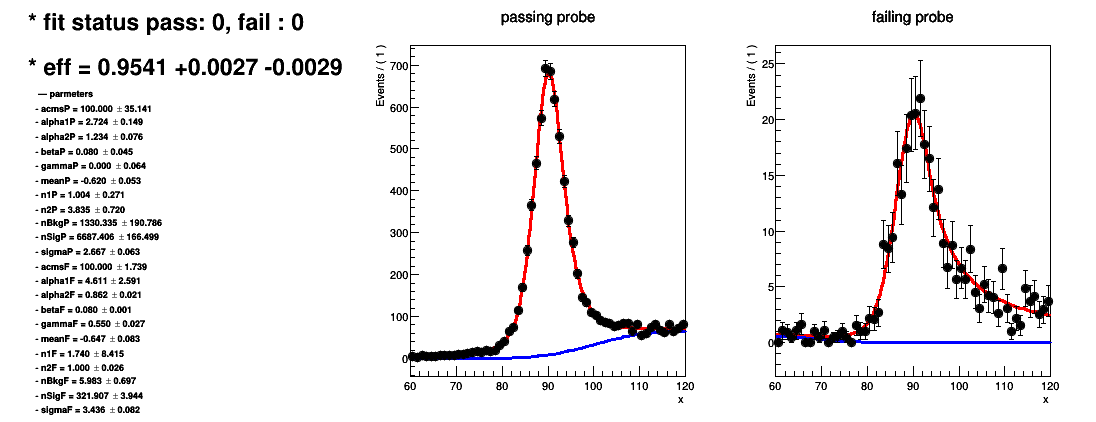
\includegraphics[height=0.355\textheight]{fits/woNF/unseed_EE_R9_0p90to0p93_et60.png}\\[2pt]
  {\scriptsize\hl{with NF}}\\[1pt]
  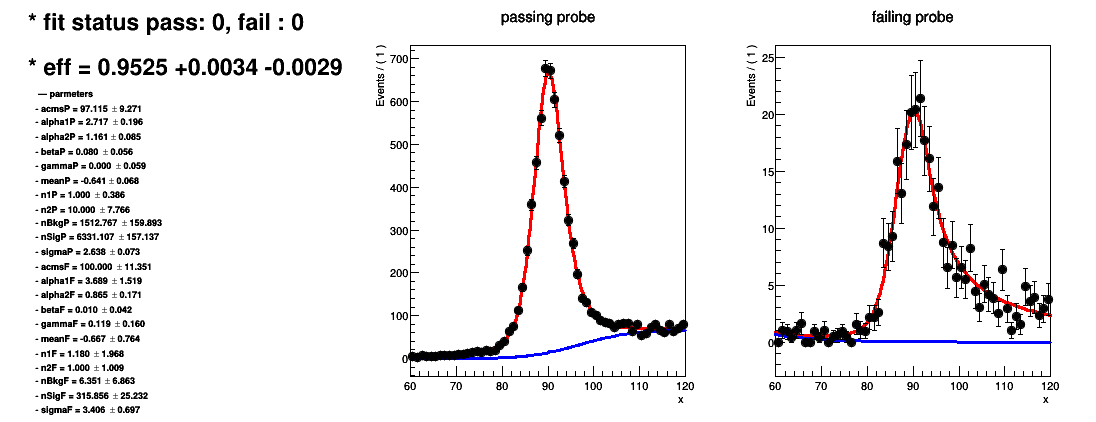
\includegraphics[height=0.355\textheight]{fits/wNF/unseed_EE_R9_0p90to0p93_et60.png}\\[2pt]
  \vspace{-10pt}\hfill\hyperlink{eff-unseed-EE}{\beamerreturnbutton{efficiency}}
\end{frame}

\begin{frame}[label=fit-unseed-EE-R9-0p90to0p93-70]{Fits: unseeded leg, EE $0.90<\RNine<0.93$, $70<\ET<90$~GeV}
  \centering
  {\scriptsize\hl{without NF}}\\[1pt]
  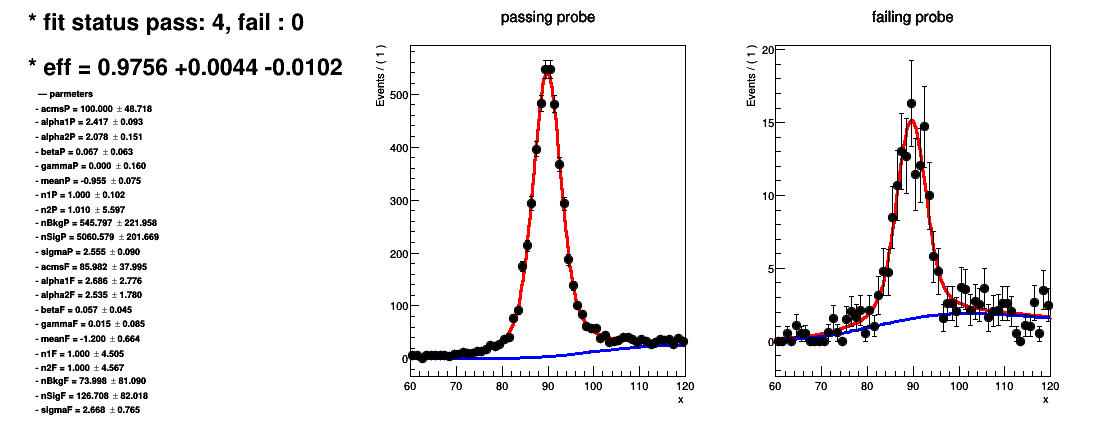
\includegraphics[height=0.355\textheight]{fits/woNF/unseed_EE_R9_0p90to0p93_et70.png}\\[2pt]
  {\scriptsize\hl{with NF}}\\[1pt]
  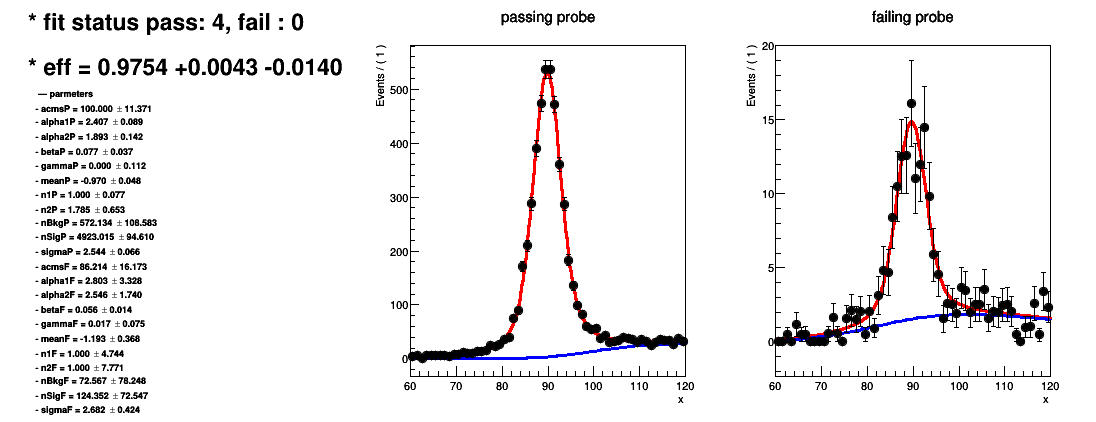
\includegraphics[height=0.355\textheight]{fits/wNF/unseed_EE_R9_0p90to0p93_et70.png}\\[2pt]
  \vspace{-10pt}\hfill\hyperlink{eff-unseed-EE}{\beamerreturnbutton{efficiency}}
\end{frame}

\begin{frame}[label=fit-unseed-EE-R9-0p90to0p93-90]{Fits: unseeded leg, EE $0.90<\RNine<0.93$, $\ET>90$~GeV}
  \centering
  {\scriptsize\hl{without NF}}\\[1pt]
  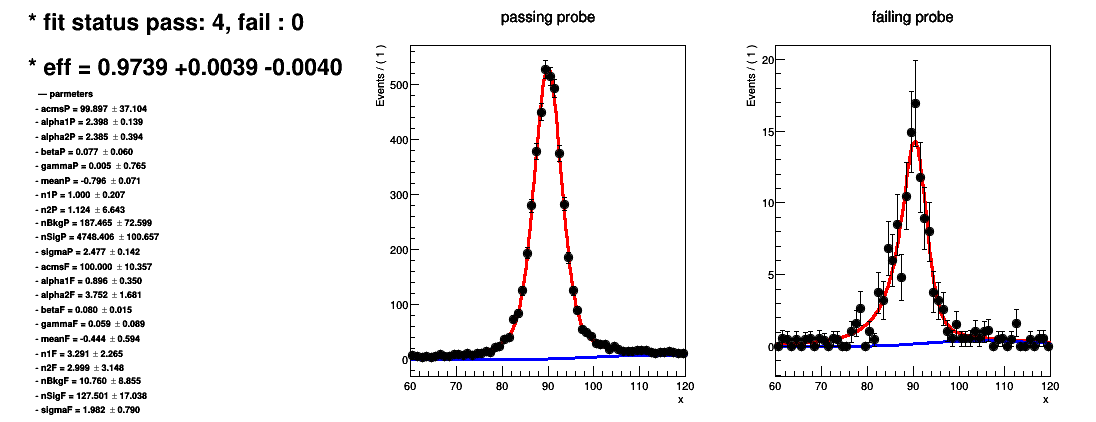
\includegraphics[height=0.355\textheight]{fits/woNF/unseed_EE_R9_0p90to0p93_et90.png}\\[2pt]
  {\scriptsize\hl{with NF}}\\[1pt]
  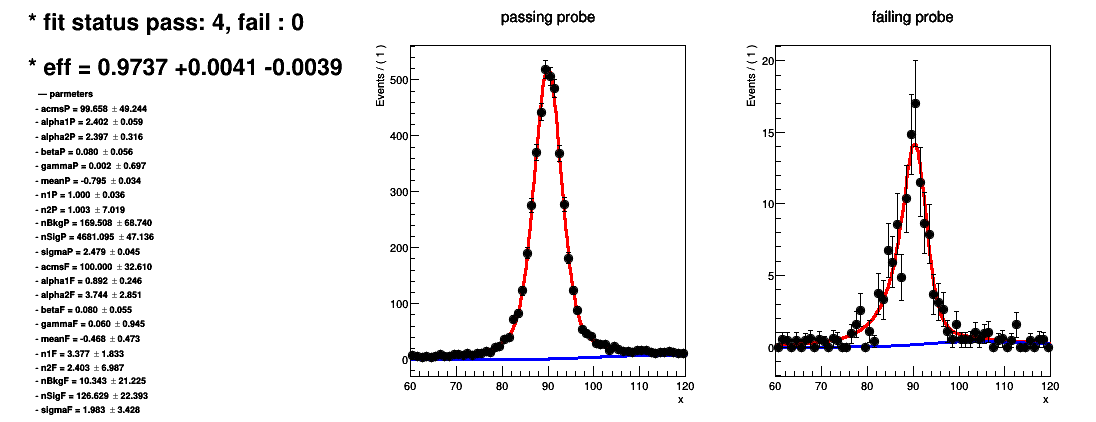
\includegraphics[height=0.355\textheight]{fits/wNF/unseed_EE_R9_0p90to0p93_et90.png}\\[2pt]
  \vspace{-10pt}\hfill\hyperlink{eff-unseed-EE}{\beamerreturnbutton{efficiency}}
\end{frame}

\begin{frame}[label=fit-unseed-EE-R9gt0p93-0]{Fits: unseeded leg, EE $\RNine>0.93$, $0<\ET<21$~GeV}
  \centering
  {\scriptsize\hl{without NF}}\\[1pt]
  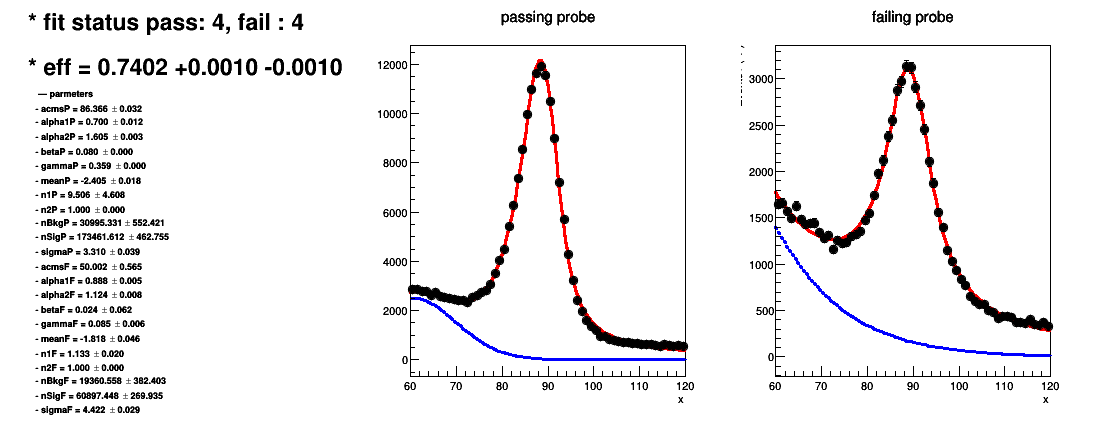
\includegraphics[height=0.355\textheight]{fits/woNF/unseed_EE_R9gt0p93_et0.png}\\[2pt]
  {\scriptsize\hl{with NF}}\\[1pt]
  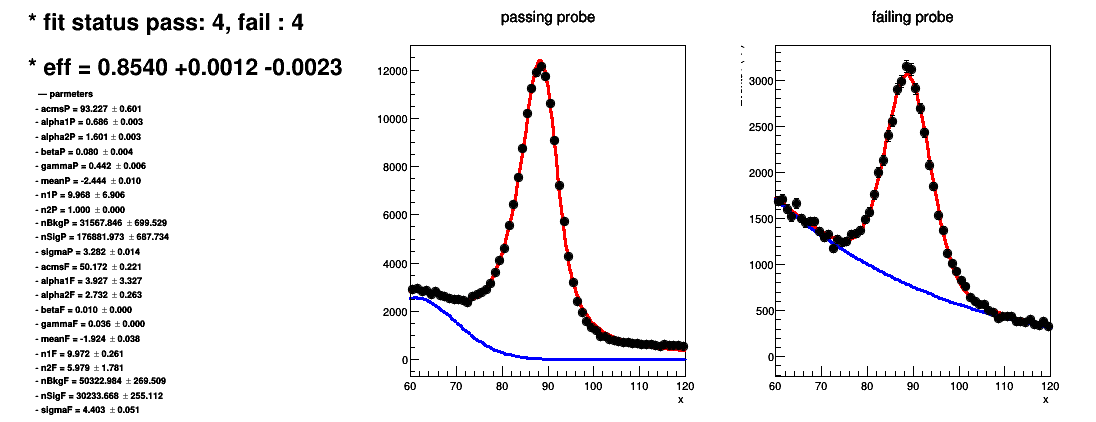
\includegraphics[height=0.355\textheight]{fits/wNF/unseed_EE_R9gt0p93_et0.png}\\[2pt]
  \vspace{-10pt}\hfill\hyperlink{eff-unseed-EE}{\beamerreturnbutton{efficiency}}
\end{frame}

\begin{frame}[label=fit-unseed-EE-R9gt0p93-21]{Fits: unseeded leg, EE $\RNine>0.93$, $21<\ET<25$~GeV}
  \centering
  {\scriptsize\hl{without NF}}\\[1pt]
  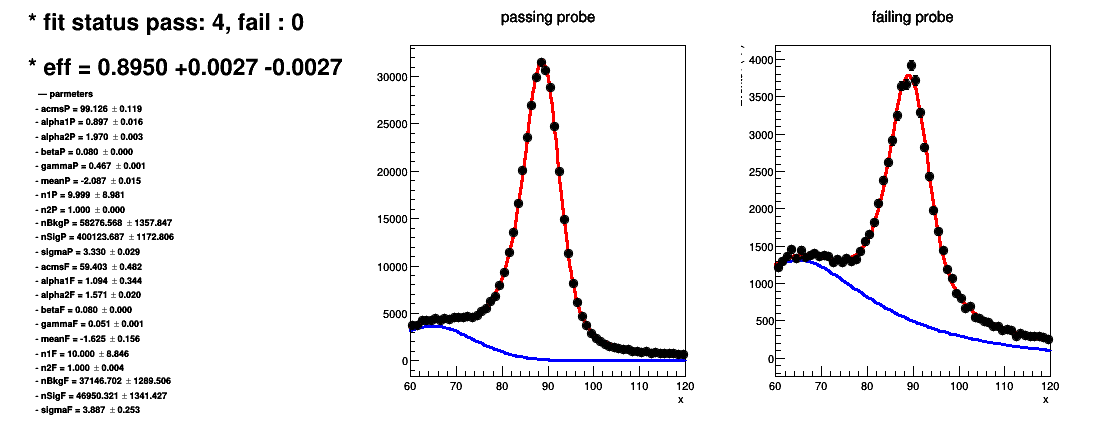
\includegraphics[height=0.355\textheight]{fits/woNF/unseed_EE_R9gt0p93_et21.png}\\[2pt]
  {\scriptsize\hl{with NF}}\\[1pt]
  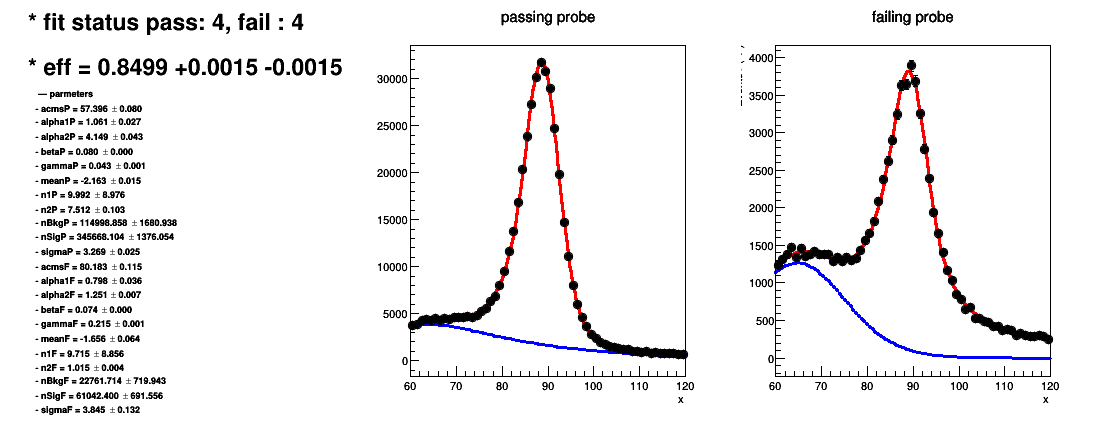
\includegraphics[height=0.355\textheight]{fits/wNF/unseed_EE_R9gt0p93_et21.png}\\[2pt]
  \vspace{-10pt}\hfill\hyperlink{eff-unseed-EE}{\beamerreturnbutton{efficiency}}
\end{frame}

\begin{frame}[label=fit-unseed-EE-R9gt0p93-25]{Fits: unseeded leg, EE $\RNine>0.93$, $25<\ET<28$~GeV}
  \centering
  {\scriptsize\hl{without NF}}\\[1pt]
  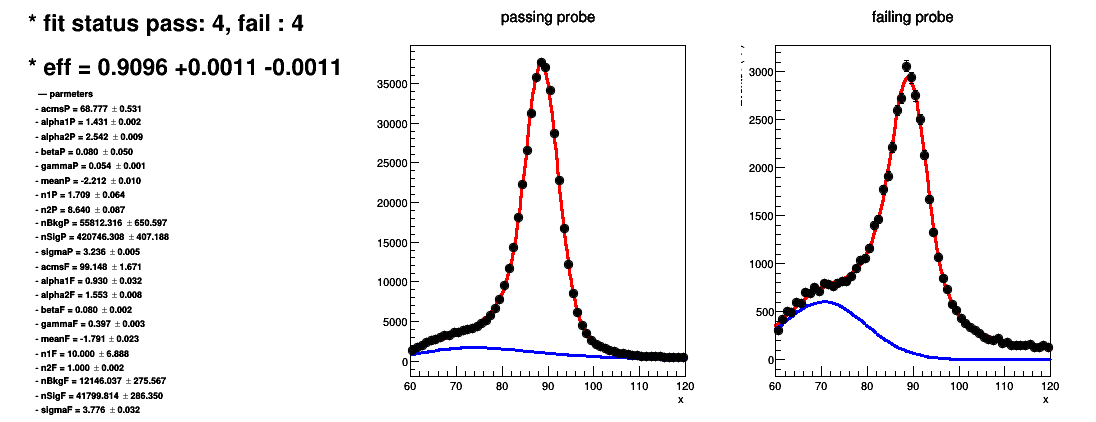
\includegraphics[height=0.355\textheight]{fits/woNF/unseed_EE_R9gt0p93_et25.png}\\[2pt]
  {\scriptsize\hl{with NF}}\\[1pt]
  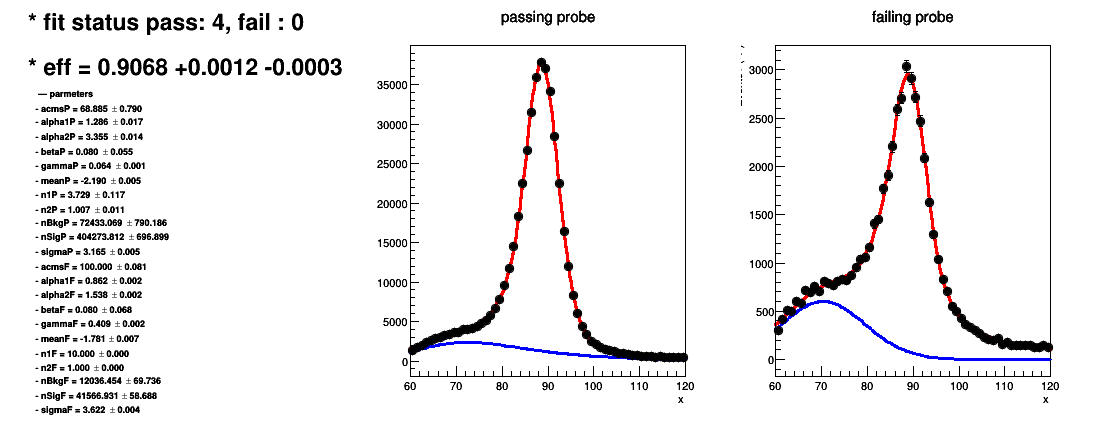
\includegraphics[height=0.355\textheight]{fits/wNF/unseed_EE_R9gt0p93_et25.png}\\[2pt]
  \vspace{-10pt}\hfill\hyperlink{eff-unseed-EE}{\beamerreturnbutton{efficiency}}
\end{frame}

\begin{frame}[label=fit-unseed-EE-R9gt0p93-28]{Fits: unseeded leg, EE $\RNine>0.93$, $28<\ET<31$~GeV}
  \centering
  {\scriptsize\hl{without NF}}\\[1pt]
  \includegraphics[height=0.355\textheight]{fits/woNF/unseed_EE_R9gt0p93_et28.png}\\[2pt]
  {\scriptsize\hl{with NF}}\\[1pt]
  \includegraphics[height=0.355\textheight]{fits/wNF/unseed_EE_R9gt0p93_et28.png}\\[2pt]
  \vspace{-10pt}\hfill\hyperlink{eff-unseed-EE}{\beamerreturnbutton{efficiency}}
\end{frame}

\begin{frame}[label=fit-unseed-EE-R9gt0p93-31]{Fits: unseeded leg, EE $\RNine>0.93$, $31<\ET<35$~GeV}
  \centering
  {\scriptsize\hl{without NF}}\\[1pt]
  \includegraphics[height=0.355\textheight]{fits/woNF/unseed_EE_R9gt0p93_et31.png}\\[2pt]
  {\scriptsize\hl{with NF}}\\[1pt]
  \includegraphics[height=0.355\textheight]{fits/wNF/unseed_EE_R9gt0p93_et31.png}\\[2pt]
  \vspace{-10pt}\hfill\hyperlink{eff-unseed-EE}{\beamerreturnbutton{efficiency}}
\end{frame}

\begin{frame}[label=fit-unseed-EE-R9gt0p93-35]{Fits: unseeded leg, EE $\RNine>0.93$, $35<\ET<40$~GeV}
  \centering
  {\scriptsize\hl{without NF}}\\[1pt]
  \includegraphics[height=0.355\textheight]{fits/woNF/unseed_EE_R9gt0p93_et35.png}\\[2pt]
  {\scriptsize\hl{with NF}}\\[1pt]
  \includegraphics[height=0.355\textheight]{fits/wNF/unseed_EE_R9gt0p93_et35.png}\\[2pt]
  \vspace{-10pt}\hfill\hyperlink{eff-unseed-EE}{\beamerreturnbutton{efficiency}}
\end{frame}

\begin{frame}[label=fit-unseed-EE-R9gt0p93-40]{Fits: unseeded leg, EE $\RNine>0.93$, $40<\ET<45$~GeV}
  \centering
  {\scriptsize\hl{without NF}}\\[1pt]
  \includegraphics[height=0.355\textheight]{fits/woNF/unseed_EE_R9gt0p93_et40.png}\\[2pt]
  {\scriptsize\hl{with NF}}\\[1pt]
  \includegraphics[height=0.355\textheight]{fits/wNF/unseed_EE_R9gt0p93_et40.png}\\[2pt]
  \vspace{-10pt}\hfill\hyperlink{eff-unseed-EE}{\beamerreturnbutton{efficiency}}
\end{frame}

\begin{frame}[label=fit-unseed-EE-R9gt0p93-45]{Fits: unseeded leg, EE $\RNine>0.93$, $45<\ET<50$~GeV}
  \centering
  {\scriptsize\hl{without NF}}\\[1pt]
  \includegraphics[height=0.355\textheight]{fits/woNF/unseed_EE_R9gt0p93_et45.png}\\[2pt]
  {\scriptsize\hl{with NF}}\\[1pt]
  \includegraphics[height=0.355\textheight]{fits/wNF/unseed_EE_R9gt0p93_et45.png}\\[2pt]
  \vspace{-10pt}\hfill\hyperlink{eff-unseed-EE}{\beamerreturnbutton{efficiency}}
\end{frame}

\begin{frame}[label=fit-unseed-EE-R9gt0p93-50]{Fits: unseeded leg, EE $\RNine>0.93$, $50<\ET<60$~GeV}
  \centering
  {\scriptsize\hl{without NF}}\\[1pt]
  \includegraphics[height=0.355\textheight]{fits/woNF/unseed_EE_R9gt0p93_et50.png}\\[2pt]
  {\scriptsize\hl{with NF}}\\[1pt]
  \includegraphics[height=0.355\textheight]{fits/wNF/unseed_EE_R9gt0p93_et50.png}\\[2pt]
  \vspace{-10pt}\hfill\hyperlink{eff-unseed-EE}{\beamerreturnbutton{efficiency}}
\end{frame}

\begin{frame}[label=fit-unseed-EE-R9gt0p93-60]{Fits: unseeded leg, EE $\RNine>0.93$, $60<\ET<70$~GeV}
  \centering
  {\scriptsize\hl{without NF}}\\[1pt]
  \includegraphics[height=0.355\textheight]{fits/woNF/unseed_EE_R9gt0p93_et60.png}\\[2pt]
  {\scriptsize\hl{with NF}}\\[1pt]
  \includegraphics[height=0.355\textheight]{fits/wNF/unseed_EE_R9gt0p93_et60.png}\\[2pt]
  \vspace{-10pt}\hfill\hyperlink{eff-unseed-EE}{\beamerreturnbutton{efficiency}}
\end{frame}

\begin{frame}[label=fit-unseed-EE-R9gt0p93-70]{Fits: unseeded leg, EE $\RNine>0.93$, $70<\ET<90$~GeV}
  \centering
  {\scriptsize\hl{without NF}}\\[1pt]
  \includegraphics[height=0.355\textheight]{fits/woNF/unseed_EE_R9gt0p93_et70.png}\\[2pt]
  {\scriptsize\hl{with NF}}\\[1pt]
  \includegraphics[height=0.355\textheight]{fits/wNF/unseed_EE_R9gt0p93_et70.png}\\[2pt]
  \vspace{-10pt}\hfill\hyperlink{eff-unseed-EE}{\beamerreturnbutton{efficiency}}
\end{frame}

\begin{frame}[label=fit-unseed-EE-R9gt0p93-90]{Fits: unseeded leg, EE $\RNine>0.93$, $\ET>90$~GeV}
  \centering
  {\scriptsize\hl{without NF}}\\[1pt]
  \includegraphics[height=0.355\textheight]{fits/woNF/unseed_EE_R9gt0p93_et90.png}\\[2pt]
  {\scriptsize\hl{with NF}}\\[1pt]
  \includegraphics[height=0.355\textheight]{fits/wNF/unseed_EE_R9gt0p93_et90.png}\\[2pt]
  \vspace{-10pt}\hfill\hyperlink{eff-unseed-EE}{\beamerreturnbutton{efficiency}}
\end{frame}


\end{document}
